\documentclass{article}
\usepackage{graphicx}
\usepackage{wrapfig}
\usepackage{amsmath}
\usepackage{verbatim}
\usepackage{makeidx}
\usepackage{float}
\usepackage{subfig}
\usepackage[left=1in,top=1in,right=1in]{geometry}

\title{Programming the Mobot}  
%\author{David Ko\\Mechanical and Aerospace Engineering}
%\date{\today} 
\makeindex

\begin{document}


\includegraphics[width=2in]{images/Barobo.png}
\hrule
\begin{center}
\vspace*{2.5cm}
{\Huge\sf\bf Mobot User's Guide}\\
\vspace*{2.5cm}
{\Large\bf Version 1.7}
\vspace{4.5cm}

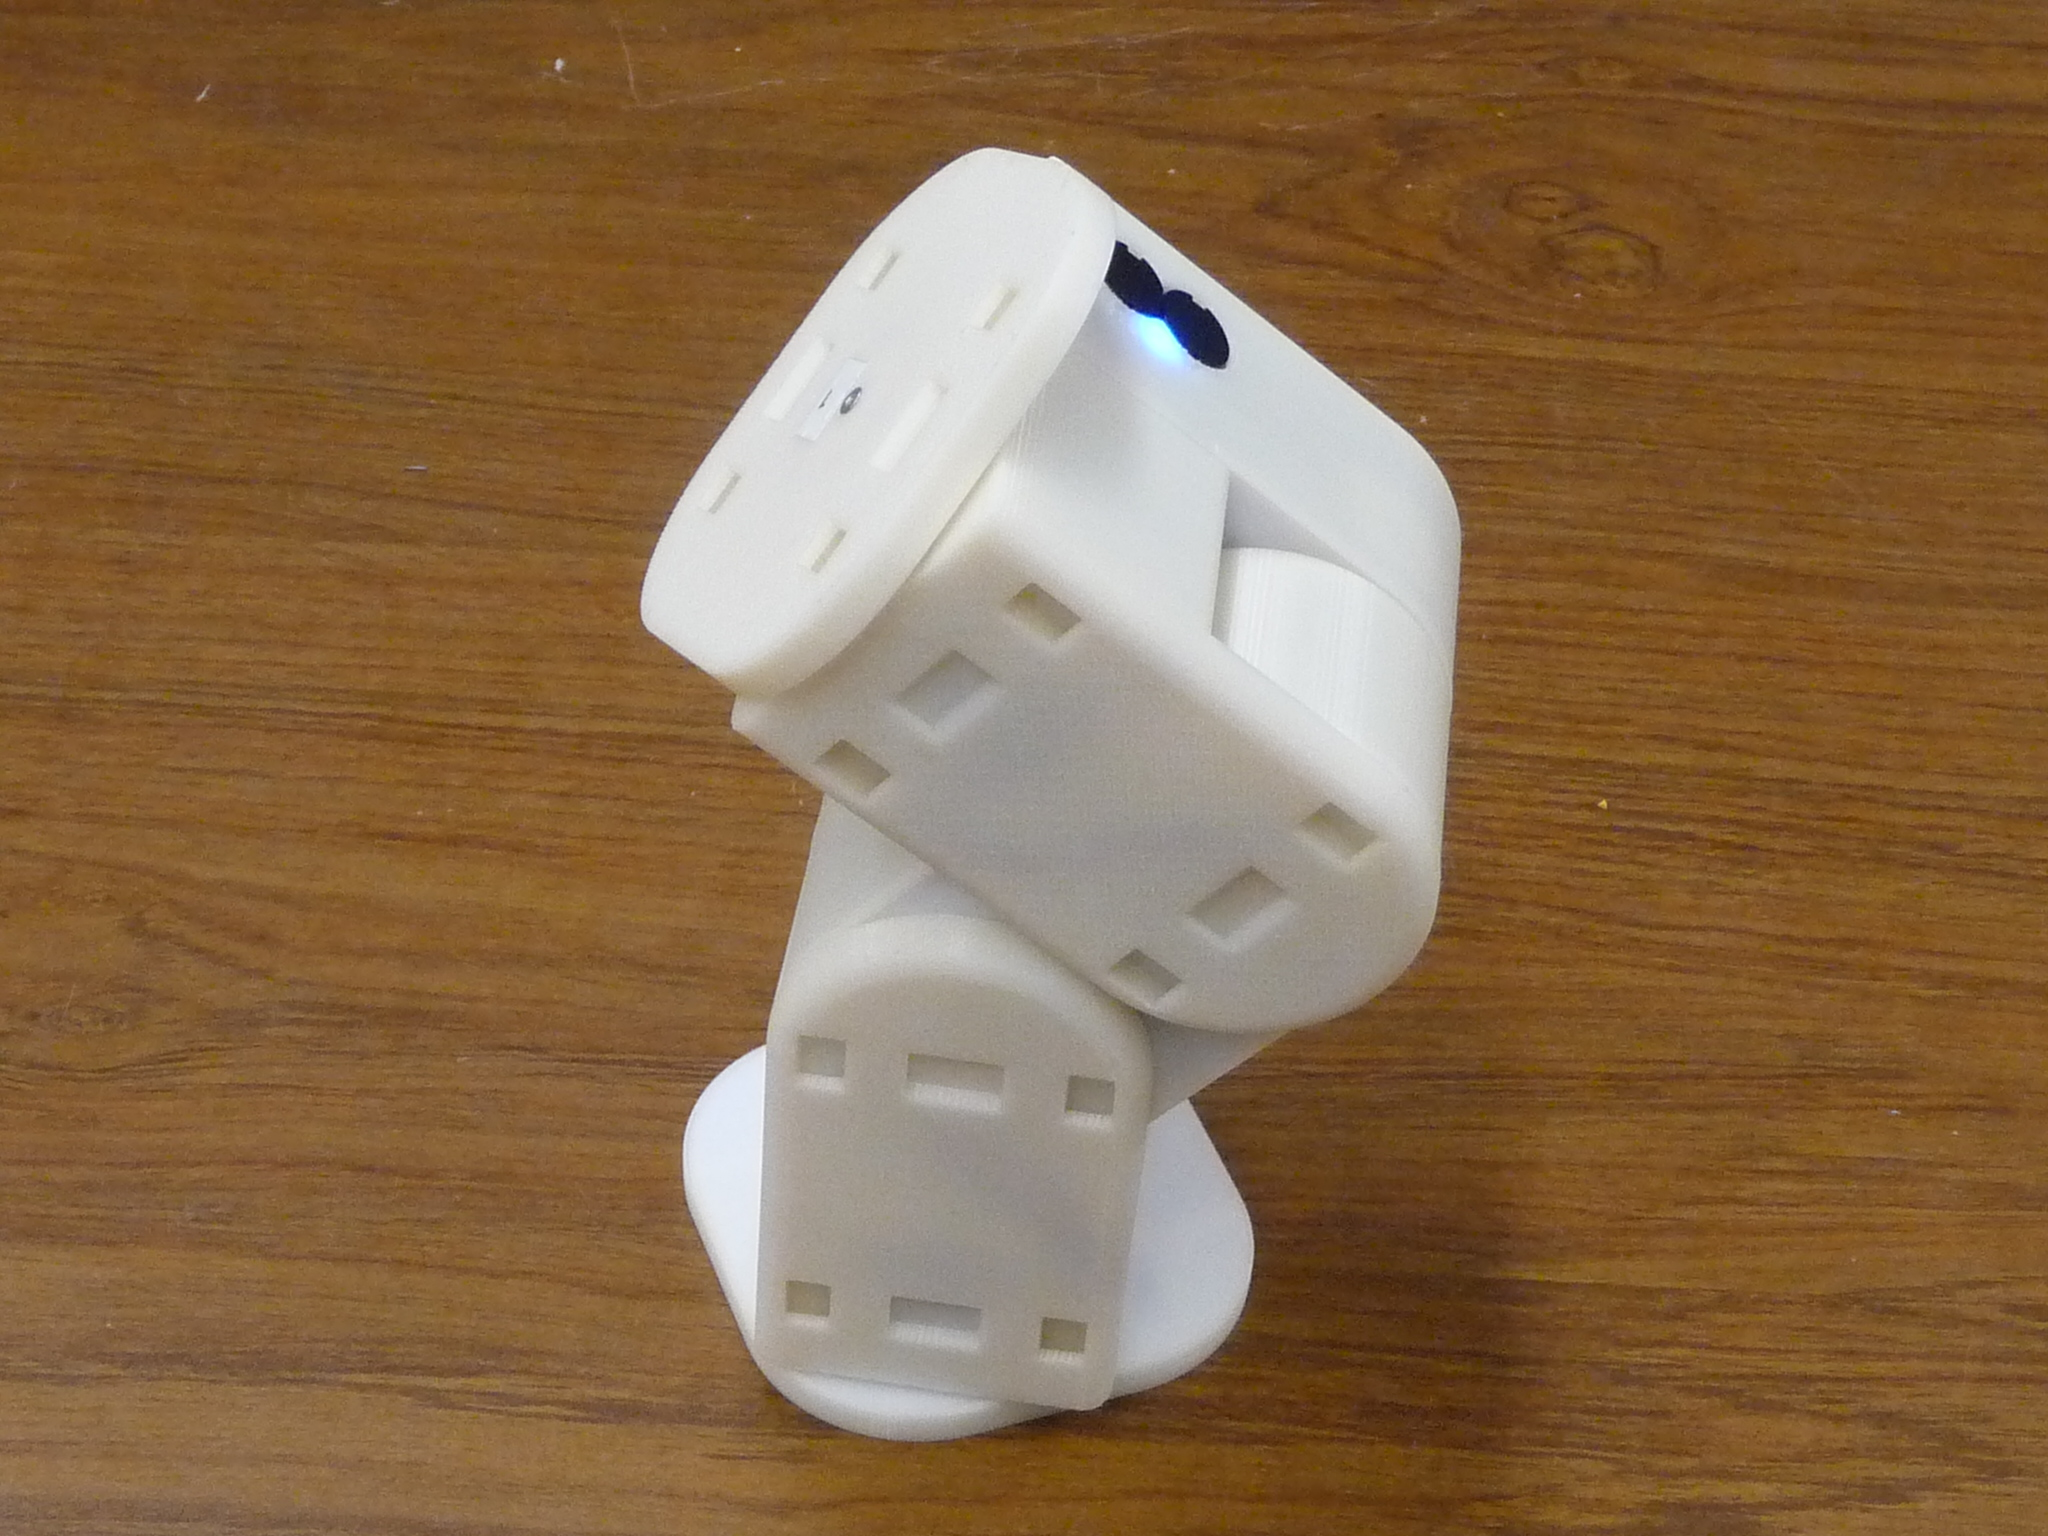
\includegraphics[width=4in]{images/Mobot_Camera_Stand.JPG}
\end{center}

\newpage
\noindent
{\large\bf How to Contact Barobo}\\
\vspace*{-6pt}

\begin{tabular} {ll}
Mail & Barobo, Inc. \\
      &813 Harbor Blvd, Suite 335\\
      &West Sacramento, CA 95691-2201\\
Phone & + 1 916 596-3050\\
%Fax & + 1 530 297 7392 \\
Web &http://www.barobo.com\\
Email &info@barobo.com 
\end{tabular}
\index{copyright}

\vspace{12pt}
\noindent
Copyright \copyright 2012 by Barobo, Inc.
All rights reserved. \\
Revision 1.4.6, March 2012\\

\noindent
Permission is granted for users to make
one copy for their own personal use. Further reproduction,
or any copying of machine-readable files (including this one)
to any server computer, is strictly prohibited.\\


\noindent
Barobo, Inc. 
is the holder of the copyright to the MoBot software
and MoBot User's Guide
described in this document, including without limitation
such aspects of the system as its code, structure,
sequence, organization, 
programming language, 
header files, 
function and command files,
object modules,
static and dynamic loaded libraries 
of object modules,
compilation of command and library names, 
interface with other languages and object modules
of static and dynamic libraries.
Use of the system unless pursuant to the terms
of a license granted by Barobo or as
otherwise authorized by law is an infringement
of the copyright.\\

\noindent
{\bf 
Barobo, Inc.
makes no representations, expressed or implied, with respect
to this documentation, or the software
it describes, including without limitations, any implied
warranty merchantability or fitness for a particular
purpose, all of which are expressly disclaimed.
Users should be aware that included in the terms and conditions
under which  Barobo is willing to license the MoBot software
as a provision that
Barobo , and their distribution
%the author, Barobo , and their distribution
licensees, distributors and dealers shall in no event
be liable for any indirect, incidental or consequential
damages in connection with, 
or arising out of, the furnishing, performance,
or use of the MoBot software
and that liability for direct damages shall be limited
to the amount of purchase price paid for MoBot and MoBot software.\\

\noindent
In addition to the foregoing, users should recognize
that all complex software systems and their documentation
%contain errors and omissions. The aand uthor and Barobo
contain errors and omissions. Barobo
shall not be responsible under any circumstances
for providing information on or corrections to errors
and omissions discovered at any time in this documentation
or the software it describes,
even if Barobo has
%even if the author and Barobo have
been advised of the errors or omissions.\\
}


\noindent
Barobo, MoBot, iMobot, and RobotController
are either
registered trademarks or trademarks of Barobo, Inc.
in the United States and/or other countries.
Ch, ChIDE, and  SoftIntegration 
are trademarks of SoftIntegrtation, Inc.
Microsoft, MS-DOS, Windows, Windows 2000, Windows XP, 
Windows Vista, and Windows 7
are trademarks of Microsoft Corporation.
Linux is a trademark of Linus Torvalds.
Mac OS X and Darwin are trademarks of Apple Computers, Inc.
All other trademarks belong to their respective holders.

%\maketitle
\newpage
\tableofcontents
\newpage
\section{Introduction}
The Mobot is a breakthrough modular robot. A single Mobot module is a fully 
functional robot capable of performing many possible motions. The Mobot
can also be used as a building block to create robots with different
geometric configurations. 
This documentation introduces the basic computer setup required for controlling 
the Mobot, as well as several demo programs and a complete reference for all
API function provided with the \texttt{CMobot} and \texttt{CMobotGroup} library.

The \texttt{CMobot} library is a collection of functions geared towards
controlling the motors and reading sensor values of a Mobot module via the
Bluetooth wireless protocol. The functions are designed to be intuitive
and easy to use. Various functions are provided to control or obtain the speed,
direction, and position of the motors. The API includes C++ classes called
\texttt{CMobot} and \texttt{CMobotGroup} to facilitate control of 
single and multiple Mobots.

\begin{figure}[H]
\begin{center}
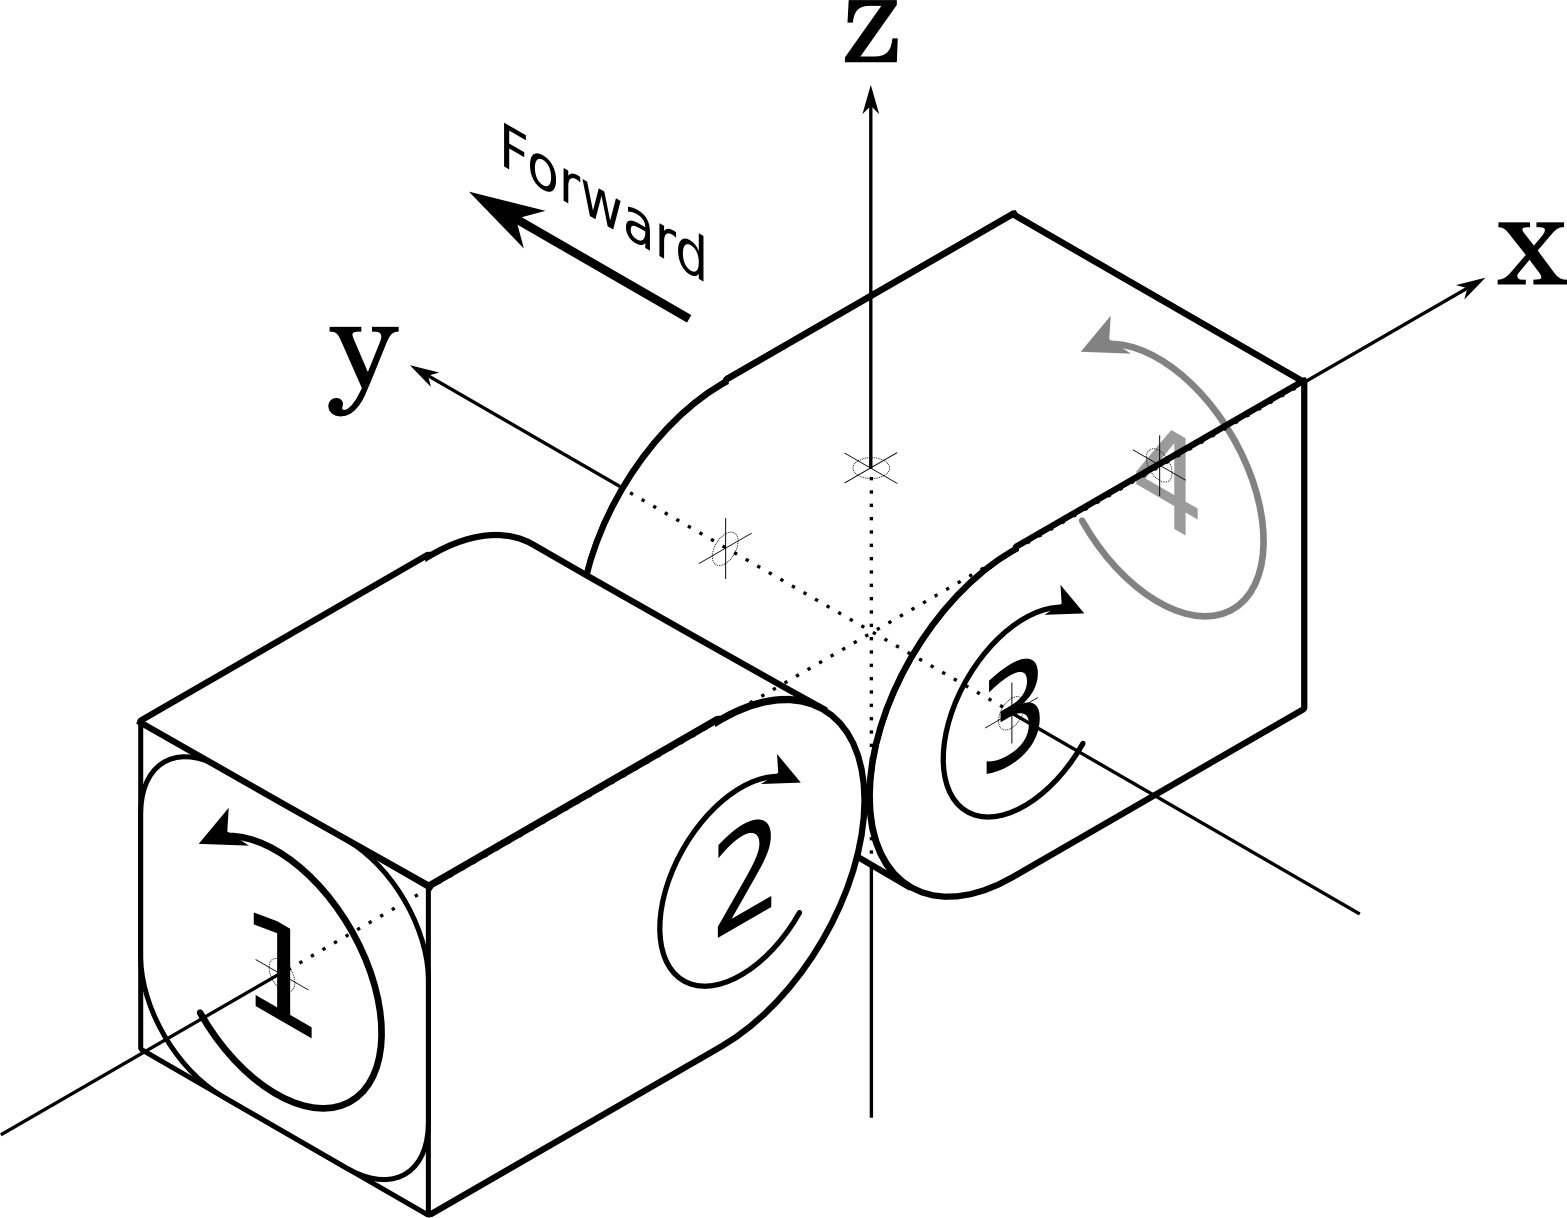
\includegraphics[width=4.5in]{images/joint_diagram_verbose.png}
\end{center}
\caption{\label{fig:joint_diagram_verbose.png} A schematic diagram of a Mobot module.}
\end{figure}

Figure \ref{fig:joint_diagram_verbose.png} shows a schematic diagram displaying the
locations and positive directions of the four joints of a Mobot module. The
joints 1 and 4 shown in the figure are fully rotational and have no joint limits.
Joints 2 and 3, however, can only move in the range -90 to +90 degrees.

\section{\label{sec:pairing}Configuring Mobots for Remote Control}
Mobot modules should be configured the first time they are used with 
a new computer. The process informs the computer which Mobots it
is allowed to connect to. The is also necessary for certain 
functions in the \texttt{CMobot} API, such as \texttt{connect()},
to determine which mobots to connect to.

The configuration is performed through the Barobo RoboMancer
program. The remainder of the section contains step-by-step instructions
and screenshots showing how to configure your Mobots.

\subsection{Bluetooth Pairing far Mac OS X}
For the Mac OS X operating system, an additional initial step needs to be performed.
Windows users may skip these steps directly to section \ref{sec:pairing_robotcontroller}
on page \pageref{sec:pairing_robotcontroller}.

To begin the pairing process, click on the Bluetooth icon on the applet tray,
typically located on the top right portion of the screen. Figure \ref{fig:mac_pairing1}
shows the Bluetooth icon on a typical Mac OS X system. Click on the icon to drop down
a menu.
\begin{figure}[H]
\begin{center}

\includegraphics[width=3in]{images/mac_pairing1.png}
\end{center}
\caption{\label{fig:mac_pairing1} The Bluetooth Icon on a Mac OS X System.}
\end{figure}

The menu that is dropped down should appear similar to the one shown in Figure \ref{fig:mac_pairing2}.
Next, click on the menu item labeled ``Set Up Bluetooth Device...''.
\begin{figure}[H]
\begin{center}
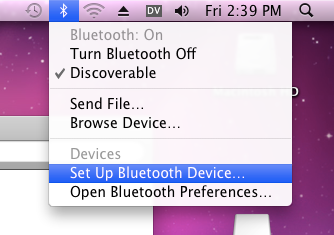
\includegraphics[width=3in]{images/mac_pairing2.png}
\end{center}
\caption{\label{fig:mac_pairing2} The Bluetooth Icon Dialog.}
\end{figure}

The previous step should start a dialog used to find and pair with Bluetooth devices. Make sure the
Mobot is turned on, and it should appear as a device in the dialog, as shown in Figure \ref{fig:mac_pairing3}.
If there are multiple Mobot devices, as shown in the figure, you may pinpoint the specific Mobot to pair
with by looking inside the battery compartment on the side of the Mobot with the power switch. Inside,
there is a sticker with the Mobot's unique ID number. The last four digits of the ID number will
coincide with the Mobot's Bluetooth ID number. Once the correct Mobot is selected, click on the ``Continue''
button.

\begin{figure}[H]
\begin{center}
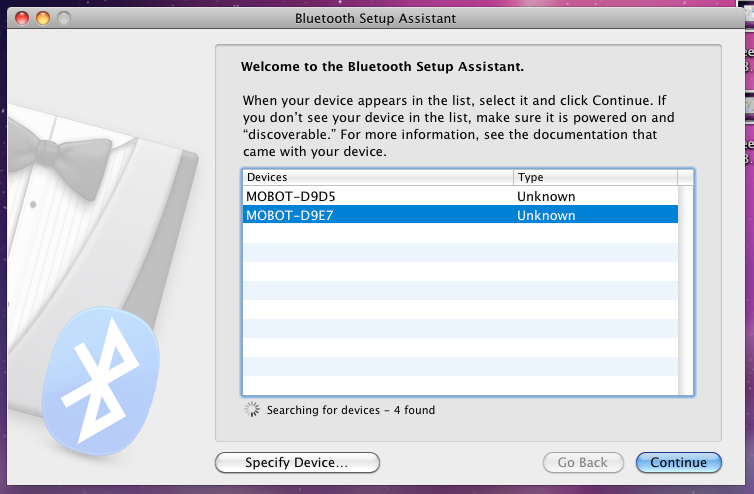
\includegraphics[width=5in]{images/mac_pairing3.png}
\end{center}
\caption{\label{fig:mac_pairing3} The Bluetooth Pairing Dialog.}
\end{figure}

At this point, the pairing dialog will attempt to pair with the Mobot using a default pairing key, ``0000'', as
shown in Figure \ref{fig:mac_pairing4}. This initial pairing attempt will fail because the Mobot pairing key
is hard-coded to a value of ``1234''. Click on the button labeled ``Passcode Options...'' in order to 
modify the passcode options. This should bring up the dialog shown in Figure \ref{fig:mac_pairing5}.

\begin{figure}[H]
\begin{center}
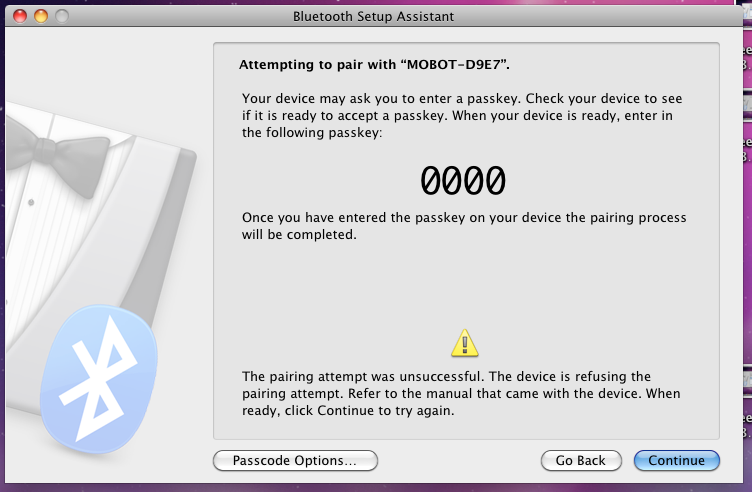
\includegraphics[width=5in]{images/mac_pairing4.png}
\end{center}
\caption{\label{fig:mac_pairing4} The Bluetooth Pairing Dialog.}
\end{figure}

\begin{figure}[H]
\begin{center}
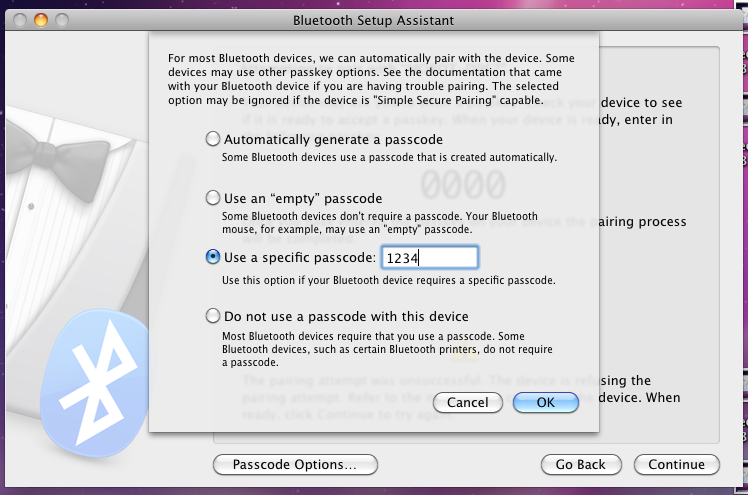
\includegraphics[width=5in]{images/mac_pairing5.png}
\end{center}
\caption{\label{fig:mac_pairing5} The Bluetooth Pairing Dialog.}
\end{figure}

In the dialog shown in Figure \ref{fig:mac_pairing5}, select the option to 
``use a specific passcode'', and enter the value ``1234''. Next, 
click on the ''OK'' button.

You should be greeted with the dialog shown in Figure \ref{fig:mac_pairing6}, which indicates that the Mobot
has successfully paired. At this point, you may continue on with the rest of the pairing process, or 
repeat this step for all Mobots that need to be paired before continuing.

\begin{figure}[H]
\begin{center}
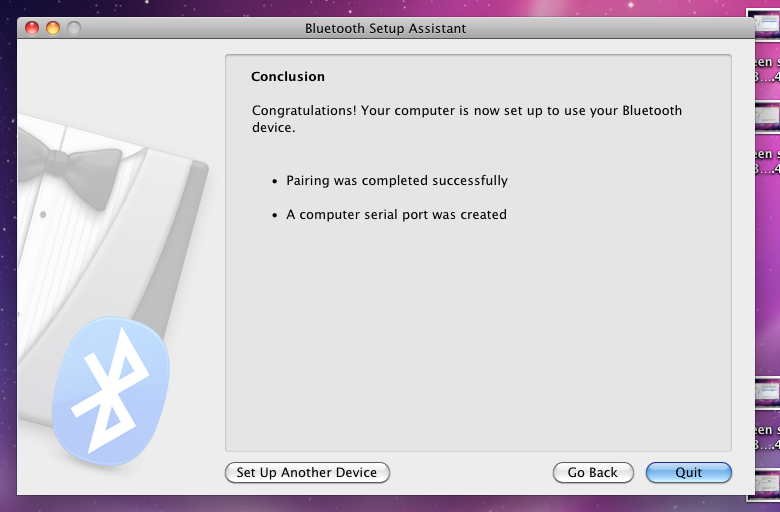
\includegraphics[width=5in]{images/mac_pairing6.png}
\end{center}
\caption{\label{fig:mac_pairing6} The Bluetooth Pairing Success Dialog.}
\end{figure}


\subsection{\label{sec:pairing_robotcontroller} Adding Bluetooth Addresses of Robots in RoboMancer.}
First, start the provided Barobo RoboMancer application.
In Windows, start the provided Barobo Robot Control Program by clicking on the icon labeled 
``RoboMancer'' on your desktop, as shown in \ref{fig:barobo_icon.png}. On Mac OS X systems,
the RoboMancer application is located inside the ``Applications'' folder in Finder. The 
control dialog as shown in Figure \ref{fig:shot1.png} should pop up.
\begin{figure}[H]
\begin{center}

\includegraphics[width=1in]{images/barobo_icon.png}
\end{center}
\caption{\label{fig:barobo_icon.png} The icon for Barobo RoboMancer.}
\end{figure}

\begin{figure}[H]
\begin{center}
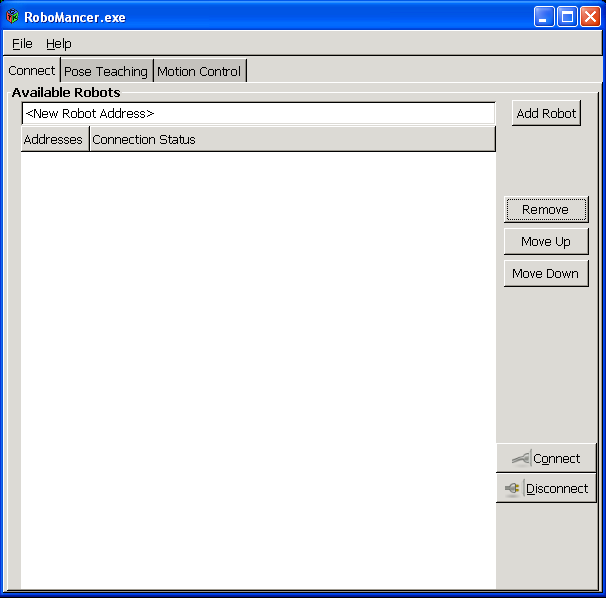
\includegraphics[width=4.5in]{images/robomancer_screenshot1.png}
\end{center}
\caption{\label{fig:shot1.png} The opening screen for RoboMancer.}
\end{figure}

The RoboMancer application, as seen in Figure \ref{fig:shot1.png}, is organized into
several different sections, each denoted by a tab. Upon startup, the default tab
that is selected is the ``Connect'' tab. This section of the application allows
you to manage, connect, and disconnect from Mobots. 

First, add your Mobot address(es) into robomancer by typing in the address and
clicking on the ``Add Robot'' button. The dialog should now something like
the figure shown in Figure \ref{fig:shot3.png}.

\begin{figure}[H]
\begin{center}
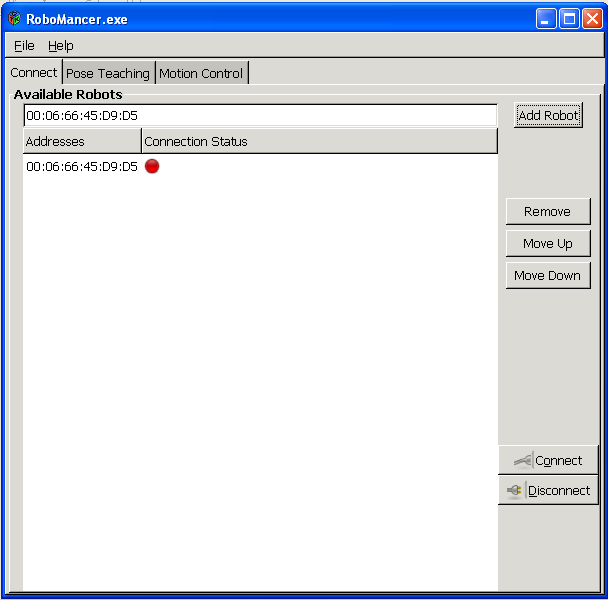
\includegraphics[width=4.5in]{images/robomancer_screenshot3.png}
\end{center}
\caption{\label{fig:shot3.png} Configuring robot bluetooth connection.}
\end{figure}

Once new addresses are added, RoboMancer will remember the addresses in the future. 
The red dot next to the added address in the ``Connection Status'' column indicates
the current connection status of the robot. The red dot indicates that the Mobot
is not currently connected, and a green dot indicates that the Mobot is 
properly connected. 

\begin{figure}[H]
\begin{center}
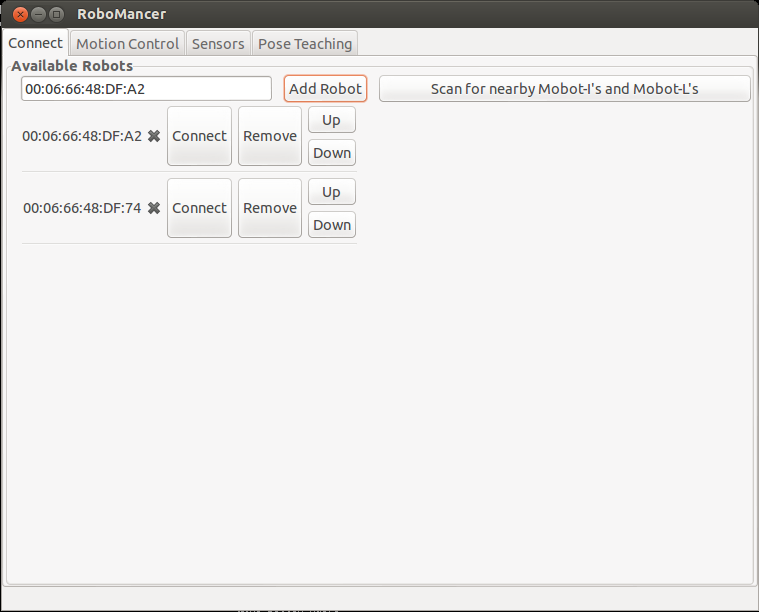
\includegraphics[width=4.5in]{images/robomancer_screenshot4.png}
\end{center}
\caption{\label{fig:shot4.png} The Connection dialog showing a connected Mobot.}
\end{figure}

To connect to your Mobot(s), select the Mobot you wish to connect to and click on
the button labelled ``Connect''. If the connection succeeds, the red dot should
turn green to indicate that a connection has been established, as shown in 
Figure \ref{fig:shot4.png}. Should the connection
fail, please check that the address has been entered correctly, the Mobot is on,
your computer has Bluetooth capability, and that the Mobot is within range of 
your computer, and try again.

Furthermore, please note that Bluetooth devices have a maximum limit of connected 
devices. The maximum limit is 7 devices connected simultaneously. This means that 
a maximum of 7 Mobots may be connected to a computer simultaneously, if no
other devices are connected. If, for instance, two other devices are currently 
connected, such as a bluetooth enabled phone and a bluetooth mouse, then the 
maximum number of connected Mobots decreases to 5, for a total of 7 connected 
devices.

\section{ The ``Motion Control'' Tab}
\begin{figure}[H]
\begin{center}
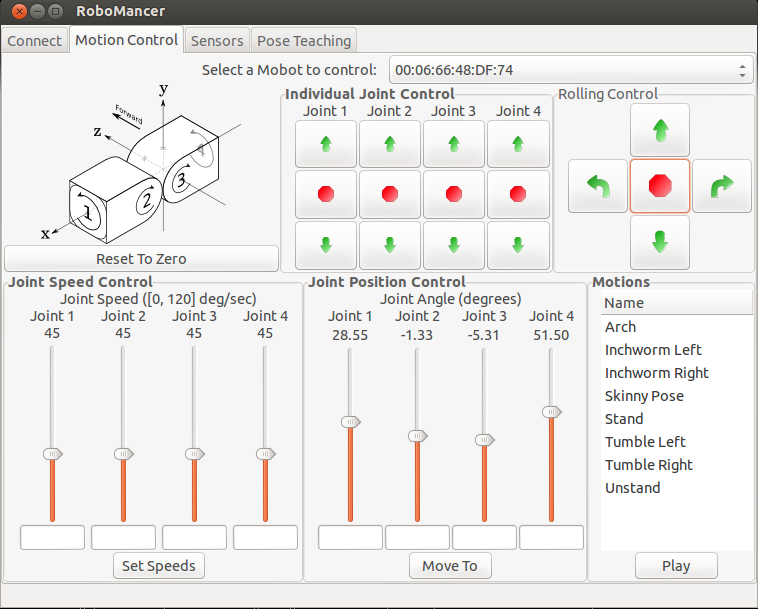
\includegraphics[width=4.5in]{images/robomancer_screenshot5.png}
\end{center}
\caption{\label{fig:shot1_populated.png} The graphical display of RoboMancer
while connected to a robot.}
\end{figure}

Once a robot is connected to RoboMancer, the joint angles and speeds
of the robot are displayed as shown in Figure \ref{fig:shot1_populated.png}.
This dialog is located under the third tab of RoboMancer, labeled 
``Motion Control''.
The ``Motion Control'' tab can be
used to display
information about the Mobot's joint positions, and also control the
speeds and positions of the Mobot's joints. The interface is divided
up into six sections; three on the top half of the interface, and three on 
the bottom half. 

\subsection{The Mobot Diagram and ``Move To Zero'' Button}
The first section of the GUI located on the top left of the interface
displays a schematic diagram of the Mobot, displaying motor positions.
Underneath the diagram, there is a large button with the text 
``Move To Zero''. When clicked, this button will command the connected
Mobot to rotate all of its joints to a flat ``Zero'' position.

It is also possible to move the Mobot into zero position using the
on-board buttons. Please refer to Section \ref{sec:zeroposition} on
page \pageref{sec:zeroposition} for more details.

\subsection{Individual Joint Control}
The second section, located at the top-middle section of the interface,
is the ``Individual Joint Control'' section. These buttons command the
Mobot to move individual joints. When the up or down arrows are clicked,
the Mobot begins to move the corresponding joint in either the positive,
or negative direction. The joint will continue to move until the stop 
button, located between the up and down arrows, is clicked. 

If the joint encounters any obstacle that prevents it from moving, the 
joint will automatically disengage power to the joint. This may happen, 
example, if a body joint attempts to rotate beyond its limits,
or if it collides with the other corresponding body joint. 

\subsection{Rolling Control}
This section contains buttons for controlling the Mobot as a 
two wheeled mobile mobot. The up and down buttons cause the Mobot to
roll forward or backward. The left and right buttons cause the Mobot 
to rotate towards the left, or towards the right. The stop button in the
middle causes the Mobot to stop where it is.

\subsection{Joint Speeds}
The ``Joint Speeds'' section, located at the bottom left of the interface,
displays and controls the current joint speeds of the Mobot.
The joint speeds are in units of degrees per second. To set a specific 
desired joint speed for a particular joint, the joint speed may be 
typed directly into the edit boxes below the sliders, and the ``Set''
button should be clicked.
 
\subsection{Joint Positions}
This section, located in the bottom-middle of the interface, is used to display
and control the positions of each of the four
joints of a Mobot. The joint positions are displayed in the numerical
text located above each vertical slider. The displayed joint positions are in
units of degrees.  
%There are two methods to control the joints using this interface.

The method of controlling the joints is by using the vertical sliders.
Each vertical slider's position represents a joint's angle. The sliders for the
two end joints vary from -180 degrees to 180 degrees, representing one complete
rotation. The angles for the two body joints vary from -90 to 90 degrees. When
the position of the slider is moved, the Mobot will move its joints to match the 
sliders. 

Underneath the sliders, there are four text entry boxes. The text boxes
accept specific angles for each joint which the user may type in. If 
the ``MoveTo'' button is clicked, each joint will move to their respective 
desired absolute positions. If any text entry is left blank, the corresponding joint will
not move. 

If the ``Move'' button is clicked, the program treats the angles entered by the
user as a relative amount to move. For instance, if the value ``360'' is entered
into the box for joint 1 and ``Move'' is clicked, the joint will rotate one full
rotation, no matter where the joint was when the motion began.
\begin{comment}
The second method for moving the joints is by entering the exact angles for the
joints. Below each of the four sliders lies a text entry box. Values in degrees
may be typed into each of the four entry boxes. When the button on the lower
right of the section labeled ``Move'' is clicked, the Mobot will move its joints
to match the values typed into the boxes. If no value is typed into a box, that 
joint will not move.
\end{comment}

\subsubsection{Joint Limits}
Joints 1 and 4 are fully rotational and have no joint limits. Joints 2 and 3, however, are 
limited to a range of -90 to +90 degrees.

\subsection{Motions}
This section, located on the bottom right of the interface, contains a set of
preprogrammed motions for the Mobot. To execute a preprogrammed motion, simply
click on the name of the motion you wish to execute, and then click the button
labeled ``Play''.

\section{The ``Pose Teaching'' Tab}
``Pose Teaching'' is the process of training a robot to perform motions by physically
moving the robot into desired positions. To pose teach a robot or multiple robots,
begin by connecting to all of the robots that will be trained by pose teaching
in the ``Connect'' tab. Once all of the desired mobots are connected, switch to
the ``Pose Teaching'' tab. Once you have switched tabs, the function of the
mobot's on-board buttons will change to Pose Teaching mode. In Pose Teaching mode,
the mobot buttons have the following functions:
\begin{itemize}
\item Button A: Record the current positions of all connected mobots.
\item Button B: Play the current recorded motions in order, or stop if motions are currently being played.
\item Buttons A and B together: Clear all recorded motions
\end{itemize}

Each time a pose is recorded, an indicator for that pose will appear in the dialog. As the
poses are played, the pose icon changes for each pose to indicate the current pose being played.

Delays may be added between poses by using the ``Add Delay'' button. The length of the delay (in seconds)
should be entered in the text box next to the ``Add Delay'' button.

It is also possible to save the recorded motion as a program by clicking on the ``Save to Program'' 
button. The generated program is a standard Ch Mobot program which may be executed 
in ChIDE. 

\section{Getting Started with Programming the Mobot}
RoboMancer can be used to control the Mobot for simple tasks and applications.
For more complicated applications, computer programs are better suited for controlling
the Mobot.
Mobot can be controlled using a C/C++ program through Ch, a C/C++ interpreter.
Ch Professional Edition or Ch Student Edition software is required to run the
demo programs for controlling Mobot. Ch is available from SoftIntegration, Inc. at
\texttt{http://www.softintegration.com}

Before the Ch program is executed, the Bluetooth addresses of the robots
need to be added using RoboMancer as described in Section \ref{sec:pairing}.

To help the user become acquainted with the Mobot control programs, sample
programs will be presented in this section to illustrate the basics and minimum requirements of
a Mobot control program. The sample programs are located at
\texttt{CHHOME/package/chmobot/demos}, where \texttt{CHHOME} is the
Ch home directory, such as \texttt{C:$\backslash$Ch} for Windows. For Windows,
it is located at \texttt{C:$\backslash$Ch$\backslash$package$\backslash$chmobot$\backslash$demos} by default.
Alternatively, the demos may be accessed in RoboMancer application
by clicking on the ``Help $\rightarrow$ Demos'' menu item, as shown in Figure
\ref{fig:help_demos_screenshot}.

\begin{figure}
  \centering
  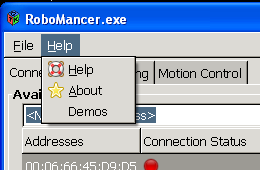
\includegraphics[width=4in]{images/help_demos_screenshot.png}
  \caption{The ``Help $\rightarrow$ Demos'' menu item on the RoboMancer Application.}
  \label{fig:help_demos_screenshot}
\end{figure}


The first demo presents a minimal program which connects to a Mobot and
moves joints 1 and 4.

\subsection{\texttt{start.ch}, A Basic Ch Mobot Program}
\subsubsection{\texttt{start.ch} Source Code}
\verbatiminput{../demos/chdemos/start.ch}

\subsubsection{\label{sec:democode}Demo Code for \texttt{start.ch} Explained}
The beginning of every Mobot control program will include header files. Each
header file imports functions used for a number of tasks, such as printing
data onto the screen or controlling the Mobot. The \texttt{mobot.h} header
file must be included in order to use the \texttt{CMobot} class and related
mobotic control functions.

\begin{verbatim}
#include <mobot.h> // Required for Mobot control functions
\end{verbatim}

Next, we must initialize the C++ class used to control the Mobot. 

\begin{verbatim}
CMobot mobot;
\end{verbatim}

This line
initializes a new variable named \texttt{mobot} which represents the remote
Mobot module which we wish to control. This special variable is actually an
instance of the \texttt{CMobot} class, which contains its own set of
functions called ``methods'', ``member functions'', or simply ``functions''.

The next line,
\begin{verbatim}
mobot.connect();
\end{verbatim}
will connect our new variable, \texttt{mobot}, to a
Mobot that has been previously configured with the computer in the 
process described in Section \ref{sec:pairing}.

Note that there are two common methods to connect to a remote Mobot. 
The most common method, demonstrated in the previous line of code, is
used to connect to a Mobot that is already paired to the computer. It
is also possible to connect to Mobots which are not paired with the 
computer. This method is necessary for connecting to multiple
Mobots simultaneously, as only a single Mobot may be paired with the
computer at a time. The second method uses the function
\texttt{connectWithAddress()}, and its default usage is as such:
\begin{verbatim}
string_t address = "11:22:33:44:55:66";
int defaultChannel = 1;
mobot.connectWithAddress(address, defaultChannel);
\end{verbatim}
The string \texttt{"11:22:33:44:55:66"} represents the Bluetooth address
of the Mobot, which must be known in advance. The channel number \texttt{1} 
represents the Bluetooth channel to connect to. Channel \texttt{1}
is the default channel Mobots listen on for incoming connections, but
may be set to other values depending on the type of mobot. Detailed
documentation for each of the Mobot functions, such as 
\texttt{connect()} and \texttt{connectAddress()}, are presented in
Appendix \ref{sec:cmobot_api}.

\begin{figure}
  \centering
  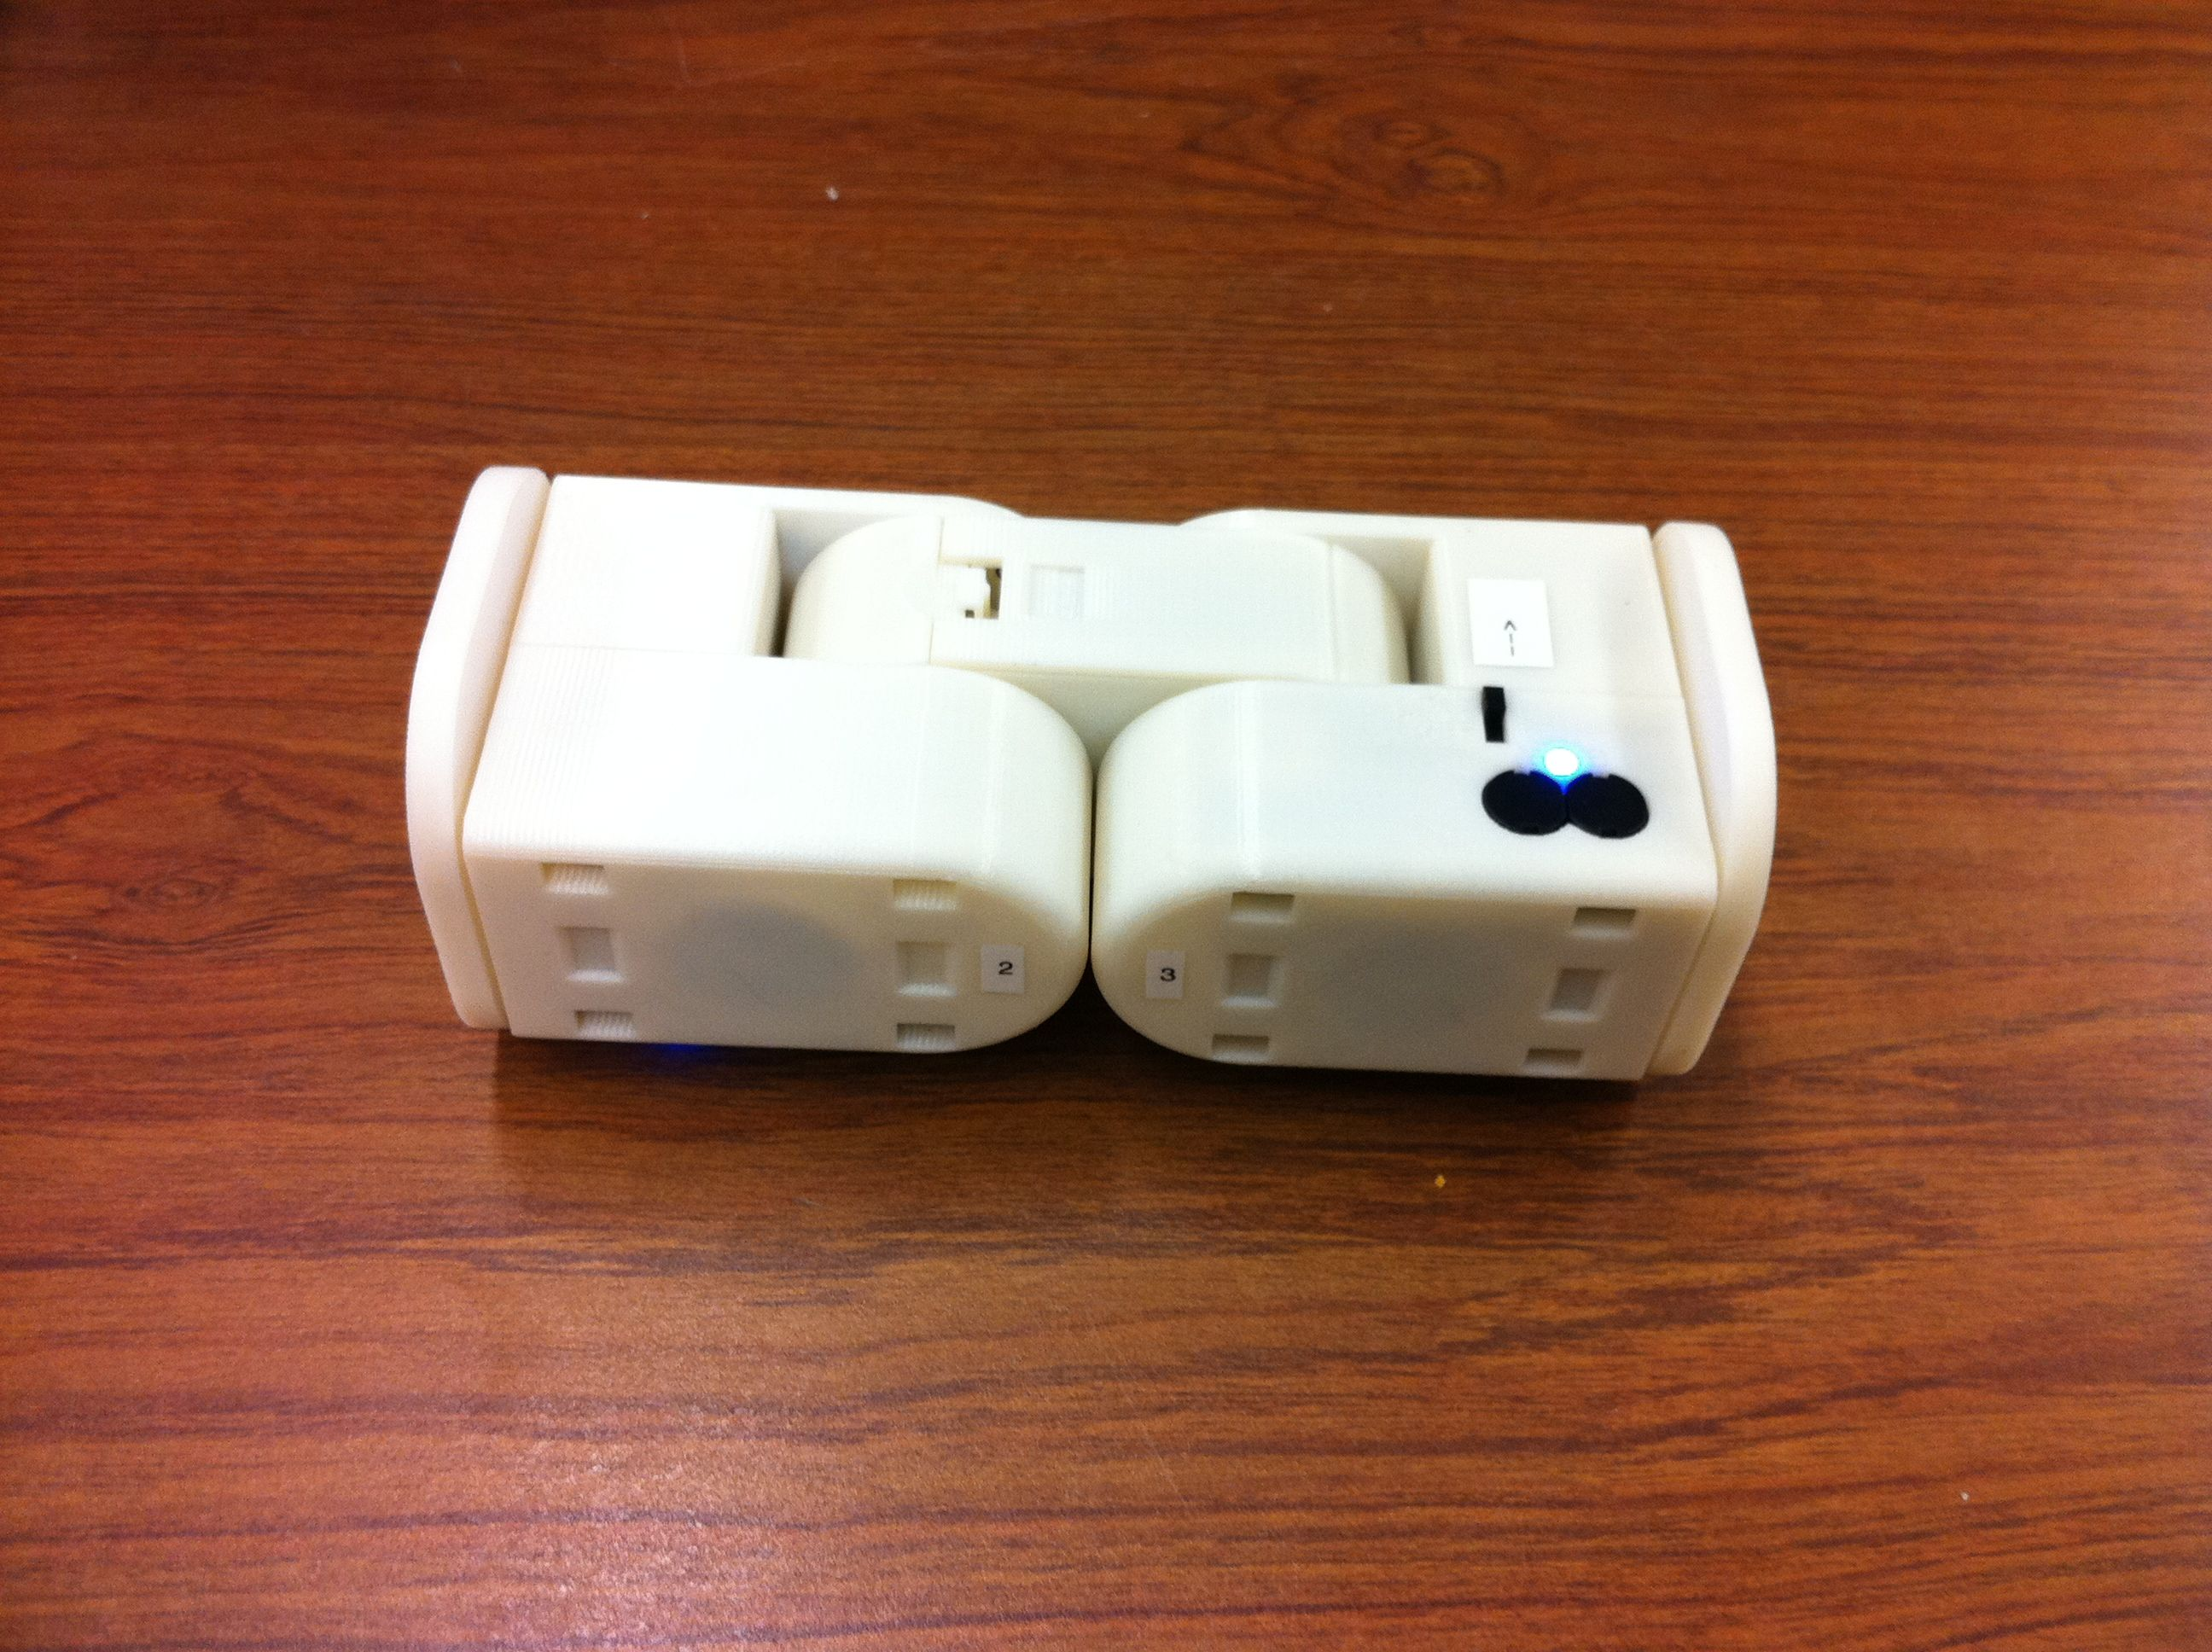
\includegraphics[width=3in]{images/inchworm1.jpg}
  \caption{The mobot in zero position}
  \label{fig:zeroposition}
\end{figure}

The next line,
\begin{verbatim}
mobot.moveToZero();
\end{verbatim}
uses the \texttt{moveToZero()} member function. The
\texttt{moveToZero} function causes the Mobot to move all of its motors to the
zero position, as shown in Figure \ref{fig:zeroposition}.

The next line of code command joints 1 and 4 to rotate 360 degrees.
\begin{verbatim}
mobot.move(360, 0, 0, 360);
\end{verbatim}
Note that the member function \texttt{move()} expects input angles
in degrees, so the angles in radians must be first be converted to degrees 
using the \texttt{rad2deg()} function. The \texttt{rad2deg()} function
takes an angle in radians as its argument and returns the angle in
degrees. The function is implemented in Ch with the code
\begin{verbatim}
#include <math.h> /* For M_PI */
double rad2deg(double radians)
{
    double degrees;
    degrees = radians * 180.0 / M_PI;
    return degrees;
}
\end{verbatim}

If desired, values in radians
may also be converted to degrees using the counterpart function,
\texttt{deg2rad()}.
Joints 1 and 4 are the faceplates
of the Mobot which are sometimes used to act as "wheels".

\subsection{\texttt{returnval.ch}, A Basic Ch Mobot Program Which Checks Return Values}
\subsubsection{Source Code}
\verbatiminput{../demos/chdemos/returnval.ch}

\subsubsection{\texttt{returnval.ch} Explained}
The first portion of the code, the lines
\begin{verbatim}
#include <mobot.h>
CMobot mobot;
\end{verbatim}
set up our program for controlling mobots as seen in previous demos. The next line,
\begin{verbatim}
double angle1, angle4;
\end{verbatim}
declares two variables that will be used to hold angle values later in the program.

The next
lines, which connect to the mobot, appear as such:
\begin{verbatim}
if(mobot.connect())
{
    printf("Failed to connect to the mobot.\n");
    exit(0);
}
\end{verbatim}
This section connects to the remote mobot as in previous examples, but also
does some error checking. The majority of the \texttt{CMobot} member functions
return an integer value indicating whether or not the function succeeded.
The \texttt{CMobot} member functions return 0 if they succeed, and -1
if any type of error has occurred. Errors may occur for any number of reasons,
including lost connections, mechanical failure, and electrical interference. 
The demos up to this point have ignored the return values of the 
\texttt{CMobot} member functions.

Next following lines,
\begin{verbatim}
/* Set the mobot to "home" position, where all joint angles are 0 degrees. */
mobot.moveToZero();

/* Rotate each of the faceplates by 360 degrees */
angle1 = 360;
angle4 = 360;
mobot.move(angle1, 0, 0, angle4);
/* Move the motors back to where they were */
angle1 = -360;
angle4 = -360;
mobot.move(angle1, 0, 0, angle4);
\end{verbatim}
move the mobot into its zero position, rotates its end plates by one full rotation, and then
rotates the end plates back to their original position. Unlike the previous demo, this 
demo uses variables to store the joint angle values. The variables are assigned 
values, and then used as the function arguments for the \texttt{move()} function.

\subsection{\texttt{getJointAngle.ch}, A Basic Ch Mobot Program Which Retrieves a Joint Angle}
\subsubsection{Source Code}
\verbatiminput{../demos/chdemos/getJointAngle.ch}

\subsubsection{\texttt{getJointAngle.ch} Explained}
The first portion of the program, 
\begin{verbatim}
#include <mobot.h>
CMobot mobot;

/* Connect to a mobot */
mobot.connect();
\end{verbatim}
initialize the mobot variable and connect to the remote mobot, as shown in the
previous demo. Next, the line
\begin{verbatim}
double angle;
\end{verbatim}
initializes a new variable called \texttt{angle}, which will be used to store
the current angle of one of the mobotic joints. The next line,
\begin{verbatim}
mobot.getJointAngle(MOBOT_JOINT1, angle);
\end{verbatim}
retrieves the current angle of joint 1, which is one of the faceplates of the
mobot. 
\texttt{MOBOT\_JOINT1} is an enumerated value
defined in the header file \texttt{mobot.h}. Detailed information
for all enumerated values defined in \texttt{mobot.h} can be found in 
Appendix \ref{sec:datatypes}.

Finally, the last line of the program,
\begin{verbatim}
printf("The current joint angle for joint 1 is %lf degrees.\n", angle);
\end{verbatim}
prints the value of the variable onto the screen. 


\section{Controlling the Speed of Mobot Joints}
\subsection{\texttt{setspeed.ch} Source Code}
\verbatiminput{../demos/chdemos/setspeed.ch}
\subsection{\texttt{setspeed.ch} Source Code Explanation}
The first several lines,
\begin{verbatim}
#include <mobot.h>
#include <math.h>

CMobot mobot;

/* Connect to the paired Mobot */
mobot.connect();

/* Set the mobot to "home" position, where all joint angles are 0 degrees. */
mobot.moveToZero();
\end{verbatim}
initialize the program, connect to the mobot, and move the mobot into its zero position,
similar to the previous demos. The next three lines,
\begin{verbatim}
double speed, radius;
mobot.getJointMaxSpeed(MOBOT_JOINT1, speed);
printf("The maximum speed is %lf degrees/s\n", speed);
\end{verbatim}
initializes the variables \texttt{speed} and \texttt{radius},
retrieves the maximum joint speed for the first joint using the member function,
\texttt{getJointMaxSpeed} and stores it in the variables named \texttt{speed}.
The value of the maximum speed is then printed onto the screen using the \texttt{printf()}
function.

The next two lines,
\begin{verbatim}
mobot.setJointSpeed(MOBOT_JOINT1, 60);
mobot.setJointSpeed(MOBOT_JOINT4, 60);
\end{verbatim}
set the joint speed settings for the two faceplate joints to 90 degrees per second.

The next lines, 
\begin{verbatim}
//mobot.setJointSpeedRatio(MOBOT_JOINT1, 0.5);
//mobot.setJointSpeedRatio(MOBOT_JOINT4, 0.5);

//mobot.setJointSpeeds(60, 0, 0, 60);
\end{verbatim}
are two alternate ways of setting the joint speeds of the faceplate joints. 
The member function \texttt{setJointSpeedRatio()} sets the joint speeds as a ratio of the 
maximum speed. The function \texttt{setJointSpeeds()} is used to set all four
joint speeds simultaneously. Note though, that there is a slight difference between
using the \texttt{setJointSpeeds()} function as shown in this example compared to the
other methods. The other methods do not alter the joint speeds for joints 2 and 3, while
the \texttt{setJointSpeeds()} function used as shown in the example explicitely sets
the joint speeds of joints 2 and 3 to zero. 

The next two lines,
\begin{verbatim}
printf("Roll forward 360 degrees.\n");
mobot.motionRollForward(360);
\end{verbatim}
print a message to the screen and rolls the mobot forward by rotating the faceplates
360 degrees.

The next lines,
\begin{verbatim}
speed = 1.83; // = (3.5/2) * M_PI * 60/180 (inch/s)
radius = 3.5/2;             // radius is 1.75 
mobot.setTwoWheelRobotSpeed(speed, radius);
\end{verbatim}
use the \texttt{setTwoWheelRobotSpeed()} function to set the faceplate joint
speeds for a mobot acting as a two wheeled car. The
\texttt{setTwoWheelRobotSpeed()} function takes a desired speed
and the radius of the wheels as arguments and calculates the necessary
rotational speed of the faceplate wheels to achieve the desired speed. Note
that the units for the speed must match the units for the radius. For instance,
if the radius is provided in inches, the desired speed must be provided in 
inches per second. If the radius is provided in centimeters, the speed must
be provided in centimeters per second, and so on. In this example, specifying 
the speed of the two wheeled mobot at 1.83 inches per second is equivalent to setting
the speeds of the two wheels at 60 degrees per second.

The following two lines,
\begin{verbatim}
printf("Move 360 degrees.\n");
mobot.move(360, 0, 0, 360);
\end{verbatim}
rotate the faceplates forward at the necessary rate to achieve a forward speed of
1.83 inches per second.

Finally, the last two lines,
\begin{verbatim}
printf("Move continuously for 3 seconds.\n");
mobot.moveContinuousTime(MOBOT_FORWARD, MOBOT_HOLD, MOBOT_HOLD, MOBOT_FORWARD, 3);
\end{verbatim}
roll the mobot forward for three seconds.
The enumerated values \texttt{MOBOT\_FORWARD} and \texttt{MOBOT\_BACKWARD}
indicate the forward and backward directions for each motor to turn, respectively. 
\texttt{MOBOT\_NEUTRAL} indicates that the motor should not turn, but
should remain flexible and backdrivable. \texttt{MOBOT\_HOLD}
indicates that the joint will not turn, and that the joint will be 
forcefully held in place at its current position. More information regarding these
macros may be found in Section \ref{sec:mobotJointState_t}. In the previous
line of code, joints 1 and 4 
move forward while joints 2 and 3 hold their current positions. The
last argument  of the function \texttt{moveContinuousTime()} specifies the
duration of time to move or hold the motors in seconds.


\section{\label{sec:preprogrammed_motions}Preprogrammed Motions}
The mobot API contains functions for executing preprogrammed motions. The 
preprogrammed motions are motions which are commonly used for mobot locomotion.
Following is a list of available functions and a brief description about
their effect on the mobot.
\begin{itemize}
\item \texttt{motionArch()}: This function causes the mobot to arch up for better 
clearance.
\item \texttt{motionInchwormLeft()}: This function causes the mobot to perform
  the inchworm gait once, moving the mobot towards its left.
\item \texttt{motionInchwormRight()}: This function causes the mobot to perform
  the inchworm gait once, moving the mobot towards its right.
\item \texttt{motionRollBackward()}: This function causes the mobot to rotate
  its faceplates, using them as wheels to roll backward.
\item \texttt{motionRollForward()}: This function causes the mobot to rotate
  its faceplates, using them as wheels to roll forward.
\item \texttt{motionSkinny()}: This function makes the mobot assume a skinnier
rolling profile.
\item \texttt{motionStand()}: This function causes the mobot to stand up onto a 
  faceplate, assuming the camera platform position.
\item \texttt{motionTumbleRight()}: This function causes the mobot to perform the
tumbling motion, flipping end over end.
\item \texttt{motionTumbleLeft()}: This function causes the mobot to perform the
tumbling motion, flipping end over end.
\item \texttt{motionTurnLeft()}: This function uses the mobot's faceplates as wheels, turning
  them in opposite directions in order to rotate the mobot towards its left.
\item \texttt{motionTurnRight()}: This function uses the mobot's faceplates as wheels, turning
  them in opposite directions in order to rotate the mobot towards its right.
\item \texttt{motionUnstand()}: This function causes the mobot to drop down from a standing position.
\end{itemize}

Note that all of the functions listed above are ``blocking'' functions, meaning
they will not return until the motion has completed. These functions also
have non-blocking equivalents which are discussed in Section
\ref{sec:blocking}.

\subsection{\texttt{inchworm.ch}: A Demo using the \texttt{motionInchwormLeft()}
Preprogrammed Motion}
\subsubsection{\texttt{inchworm.ch} Source Code}
\verbatiminput{../demos/chdemos/inchworm.ch}
\subsubsection{\texttt{inchworm.ch} Explained}
First, the header file \texttt{mobot.h} is included. This header file
is required before usage of the \texttt{CMobot} class and its associated
member functions can be used. Next, we create a variable to reperesent our
mobot and connect to the mobot with the following lines.
\begin{verbatim}
CMobot mobot;

/* Connect to the paired Mobot */
mobot.connect();
\end{verbatim}

Next, we set the motor speeds to 50\% speed with the following lines.
\begin{verbatim}
mobot.setJointSpeedRatio(MOBOT_JOINT2, 0.50);
mobot.setJointSpeedRatio(MOBOT_JOINT3, 0.50);
\end{verbatim}

We then move the mobot to its zero position in preparation for the 
inchworm gait.
\begin{verbatim}
mobot.moveToZero();
\end{verbatim}

Finally, we perform the inchworm gait four times. The argument for the
function \texttt{motionInchwormLeft()} reperesents the number of times
the gait should be performed.
\begin{verbatim}
mobot.motionInchwormLeft(4);
\end{verbatim}


\subsection{\texttt{stand.ch}: A Demo Using the \texttt{motionStand()} Preprogrammed
Motion}
This demo is a simple demonstration of the \texttt{motionStand()} member function.
\subsubsection{\texttt{stand.ch} Source Code}
\verbatiminput{../demos/chdemos/stand.ch}
\subsubsection{\texttt{stand.ch} Explained}
After the initialization and 
connection as seen in the previous demo, it executes the following line of
code:
\begin{verbatim}
mobot.motionStand();
\end{verbatim}
This line of code causes the Mobot to perform a sequence of motions causing it to
stand up on a faceplate. After the mobot has stood up, the next line of code,
\begin{verbatim}
delay(3); // Stand still for three seconds
\end{verbatim}
pauses the program for three seconds, causing the mobot to remain still for three
seconds. 

After the pause is over, the line
\begin{verbatim}
mobot.move(2*360, 0, 0, 2*360);
\end{verbatim}
turns both faceplates of the mobot two full rotations, making the mobot spin in place
while standing. Finally, the line
\begin{verbatim}
mobot.motionUnstand();
\end{verbatim}
causes the mobot to drop back down into a flat position.

\subsection{\texttt{tumble.ch}: A Demo Using the \texttt{motionTumbleLeft()} Preprogrammed
Motion}
\subsubsection{\texttt{tumble.ch} Source Code}
\verbatiminput{../demos/chdemos/tumble.ch}
\subsubsection{\texttt{tumble.ch} Explained}
The first portion of the program,
\begin{verbatim}
/* Filename: tumble.ch 
 * Tumbling mobot */
#include <mobot.h>
CMobot mobot;

/* Connect to the paired Mobot */
mobot.connect()
/* Set the mobot to "home" position, where all joint angles are 0 degrees. */
mobot.moveToZero();
\end{verbatim}
initialize the proper variables, connect to the remote mobot, and make it move
to a flat zero position, similar to previous demos.

Next, we make the mobot perform the tumbling motion with the following line:
\begin{verbatim}
mobot.motionTumbleLeft(2);
\end{verbatim}
The argument, ``2'', indicates that the tumbling motion should be performed
two times.

\subsection{\texttt{motion.ch}: A Demo Using Multiple Preprogrammed Motions}
\subsubsection{\texttt{motion.ch} Source Code}
\verbatiminput{../demos/chdemos/motion.ch}
\subsubsection{\texttt{motion.ch} Explained}
The first portion of the program initializes and connects to the
remote mobot similar to the previous demos.

The next portion of code executes a number of different pregrammed motions
to demonstrate the motion capabilities of the mobot. First, the ``Arch'' motion
is demonstrated by the following line of code:
\begin{verbatim}
mobot.motionArch(15);
\end{verbatim}
The parameter given to the function, ``15'' in this case, is the angle in degrees 
that the body joints should form in relation to each other. 

The next couple lines of code,
\begin{verbatim}
mobot.motionInchwormLeft(4);
mobot.motionInchwormRight(4);
\end{verbatim}
make the mobot inchworm to the left four times, and then inchworm to the right
four times. 

Next, the lines
\begin{verbatim}
mobot.motionRollBackward(360);
mobot.motionRollForward(360);
mobot.motionTurnLeft(360);
mobot.motionTurnRight(360);
\end{verbatim}
make the mobot roll backward, forward, and then turn left, and turn right
sequentially. For each of these functions, the parameter is the angle in degrees
to turn the faceplates. For instance, the line rolls the mobot backward
using its faceplates as wheels by rotating the faceplates 360 degrees.

Next, the mobot stands up by executing the line
\begin{verbatim}
mobot.motionStand();
\end{verbatim}

While the mobot is standing, the line
\begin{verbatim}
mobot.move(360, 0, 0, 360);
\end{verbatim}
rotates both faceplates one complete rotation. This causes the mobot to spin around 
in a circle, since it is currently standing on one of its faceplates.

Next, we lay the mobot back down into a prone position with the following line
of code:
\begin{verbatim}
mobot.motionUnstand();
\end{verbatim}

Finally, we perform the tumbling motion. 
\begin{verbatim}
mobot.motionTumbleLeft(2);
\end{verbatim}
The tumbling motion is a movement in which
the mobot stands up and then flips, end over end. The argument provided to the
function, ``2'' in this case, is the number of times to perform the motion.

\section{Detailed Examples of Preprogrammed Motions and Writing Customized Motions}
In the previous sections, preprogrammed motions have been demonstrated. In this section,
the inner workings of the preprogrammed motions will be discussed, as well as various
methods of designing and creating custom motions. Some more complex motions, such as 
``motionTumbleLeft()'' and ``motionUnstand()'' will be discussed in Section \ref{sec:blocking}.
\subsection{Inchworm Gait Demo}
The next demo will illustrate how a simple gait known as the ``Inchworm'' gait 
can be implemented.

\subsubsection{\texttt{inchworm2.ch} Source Code}
\verbatiminput{../demos/chdemos/inchworm2.ch}

\subsubsection{Demo Code for \texttt{inchworm2.ch} Explained}
The first portion of the code is identical to the previous demo, and performs
the same function of declaring a Mobot variable and connecting to a 
paired Mobot.
\begin{verbatim}
#include <mobot.h>
CMobot mobot;

/* Connect to the paired Mobot */
mobot.connect();
\end{verbatim}

The next lines of code set the joint speeds for the two body joints, joints 
2 and 3, to 50\% speed. They are set to fifty percent speed in order to 
slow the motion down in order to minimize slippage.

\begin{verbatim}
/* Set mobot motors to speed of 0.50 */
mobot.setJointSpeedRatio(MOBOT_JOINT2, 0.50);
mobot.setJointSpeedRatio(MOBOT_JOINT3, 0.50);
\end{verbatim}

Next, we move the mobot into a flat ``zero'' position, as shown in Figure \ref{fig:inchworm1}.

\begin{verbatim}
/* Set the mobot to "home" position, where all joint angles are 0 degrees. */
mobot.moveToZero();
\end{verbatim}

\begin{figure}
  \centering
  \subfloat[Zero Position]{\label{fig:inchworm1}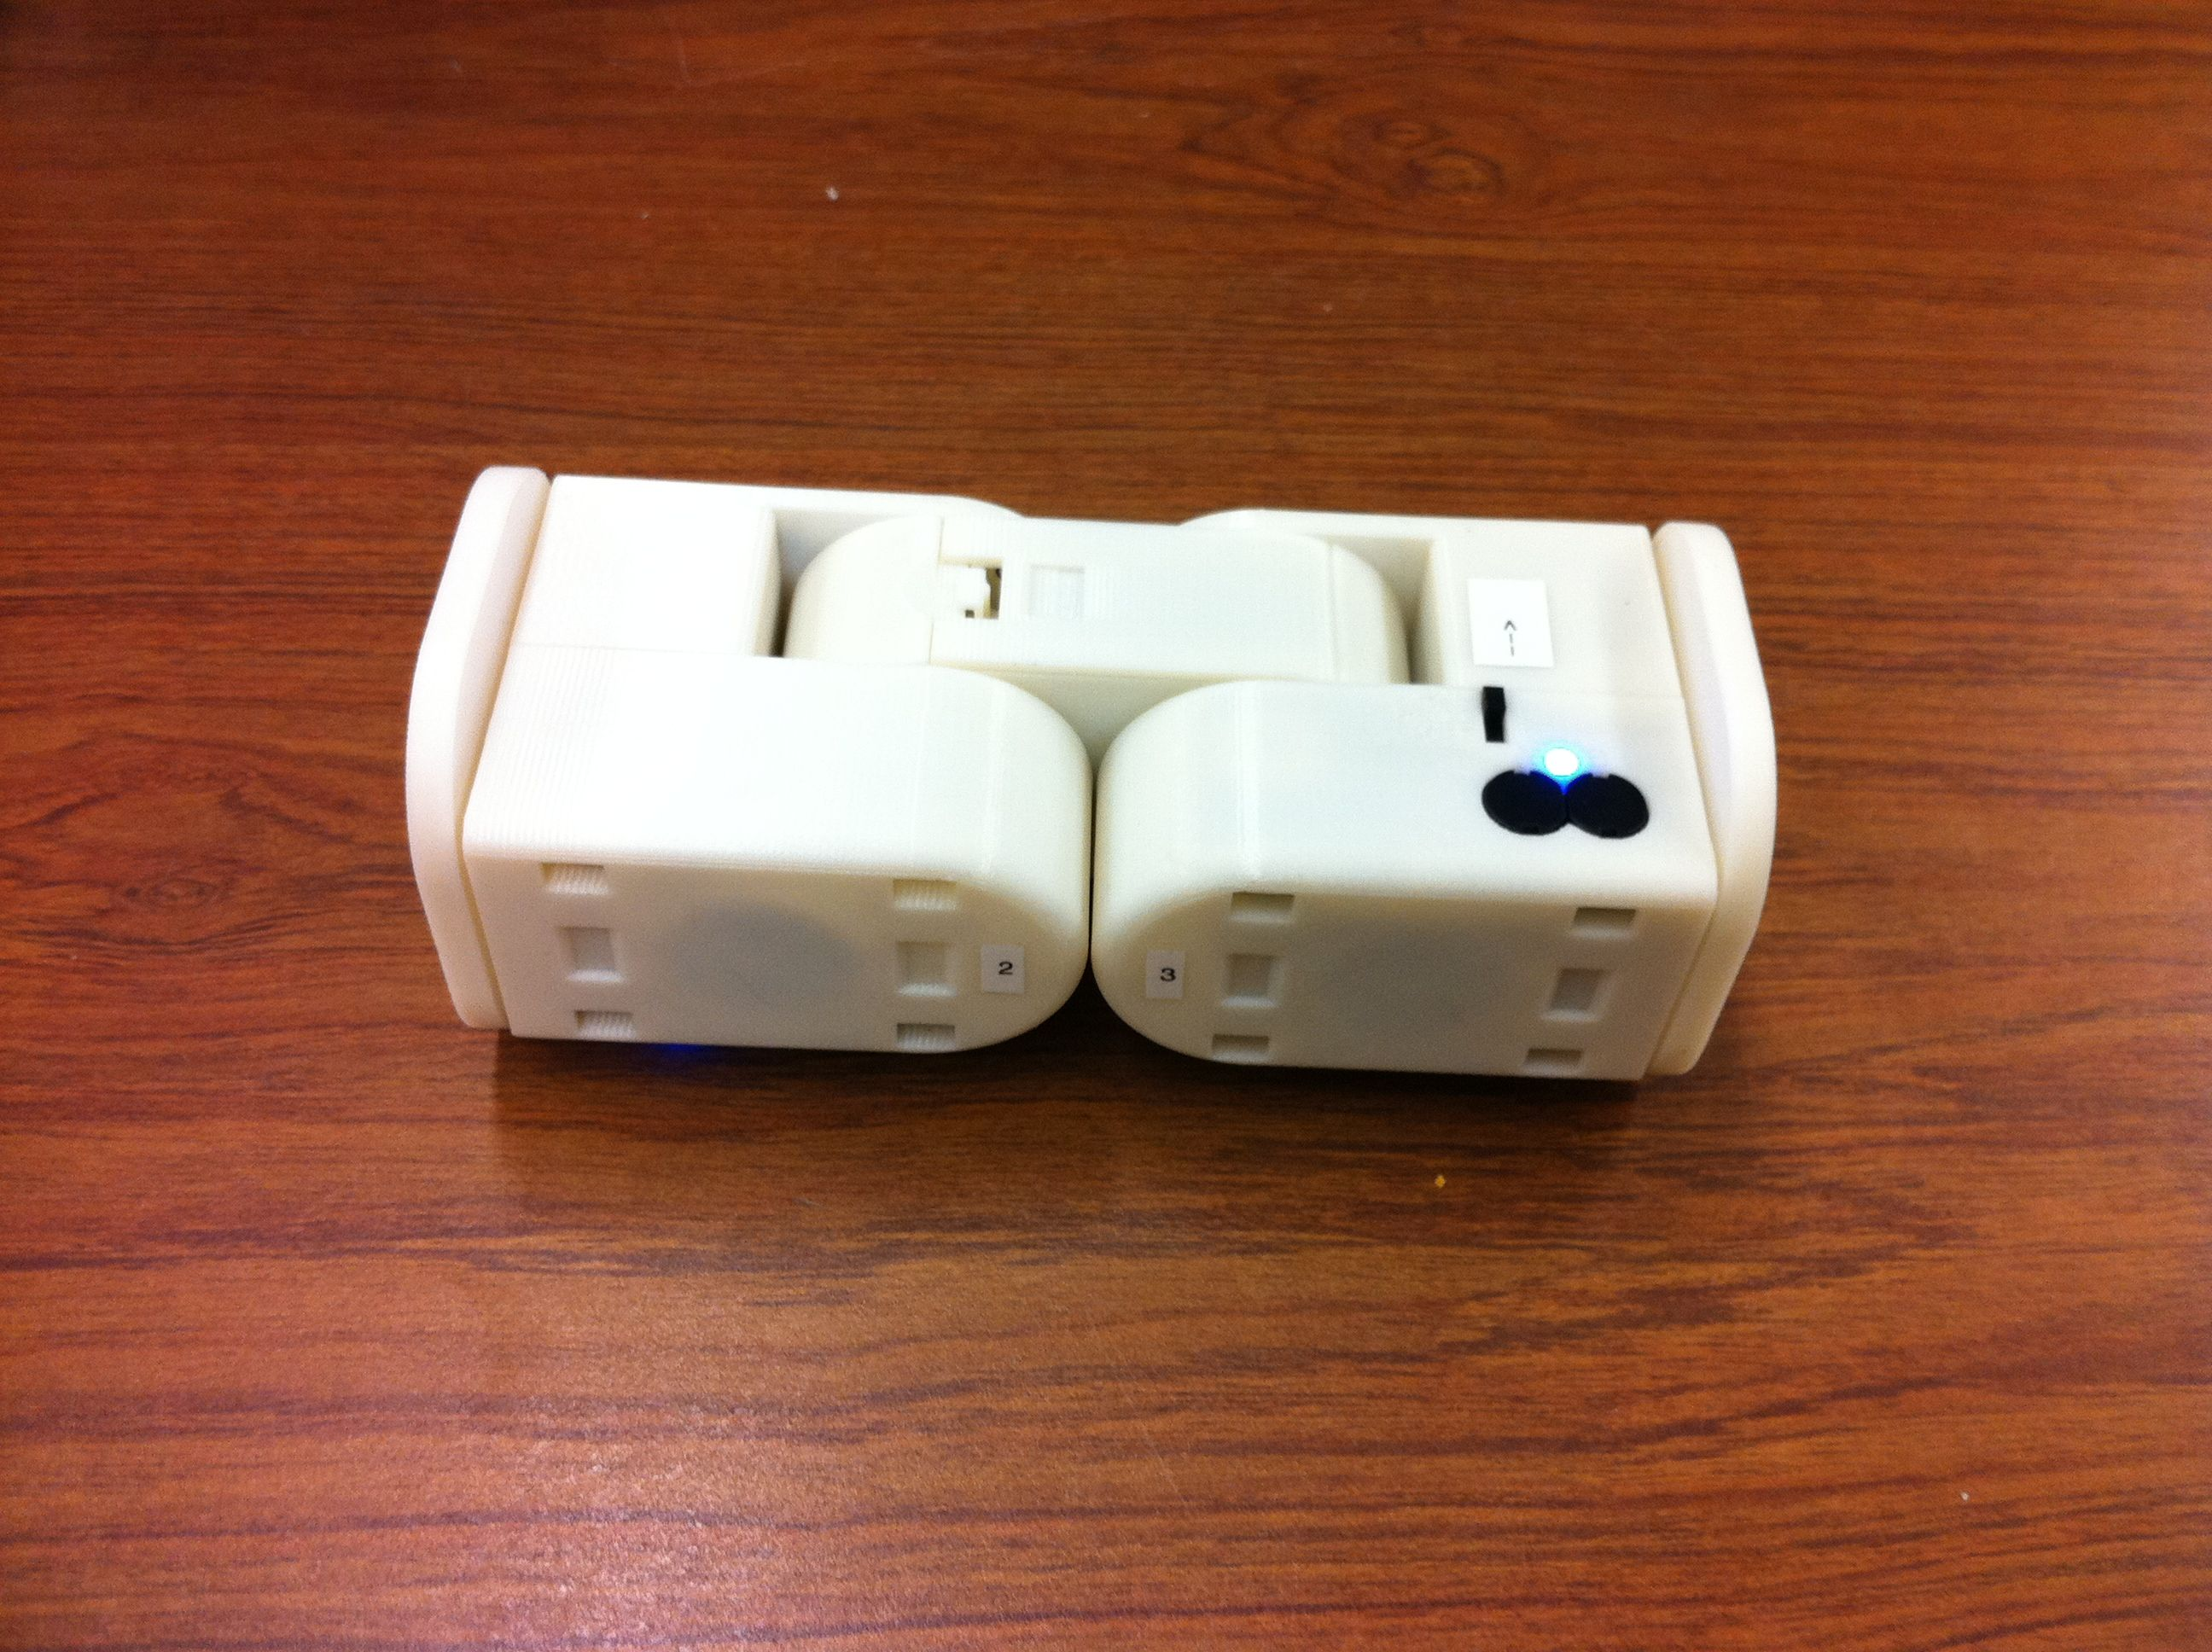
\includegraphics[width=1in]{images/inchworm1.jpg}}
  \subfloat[Move joint 2]{\label{fig:inchworm2}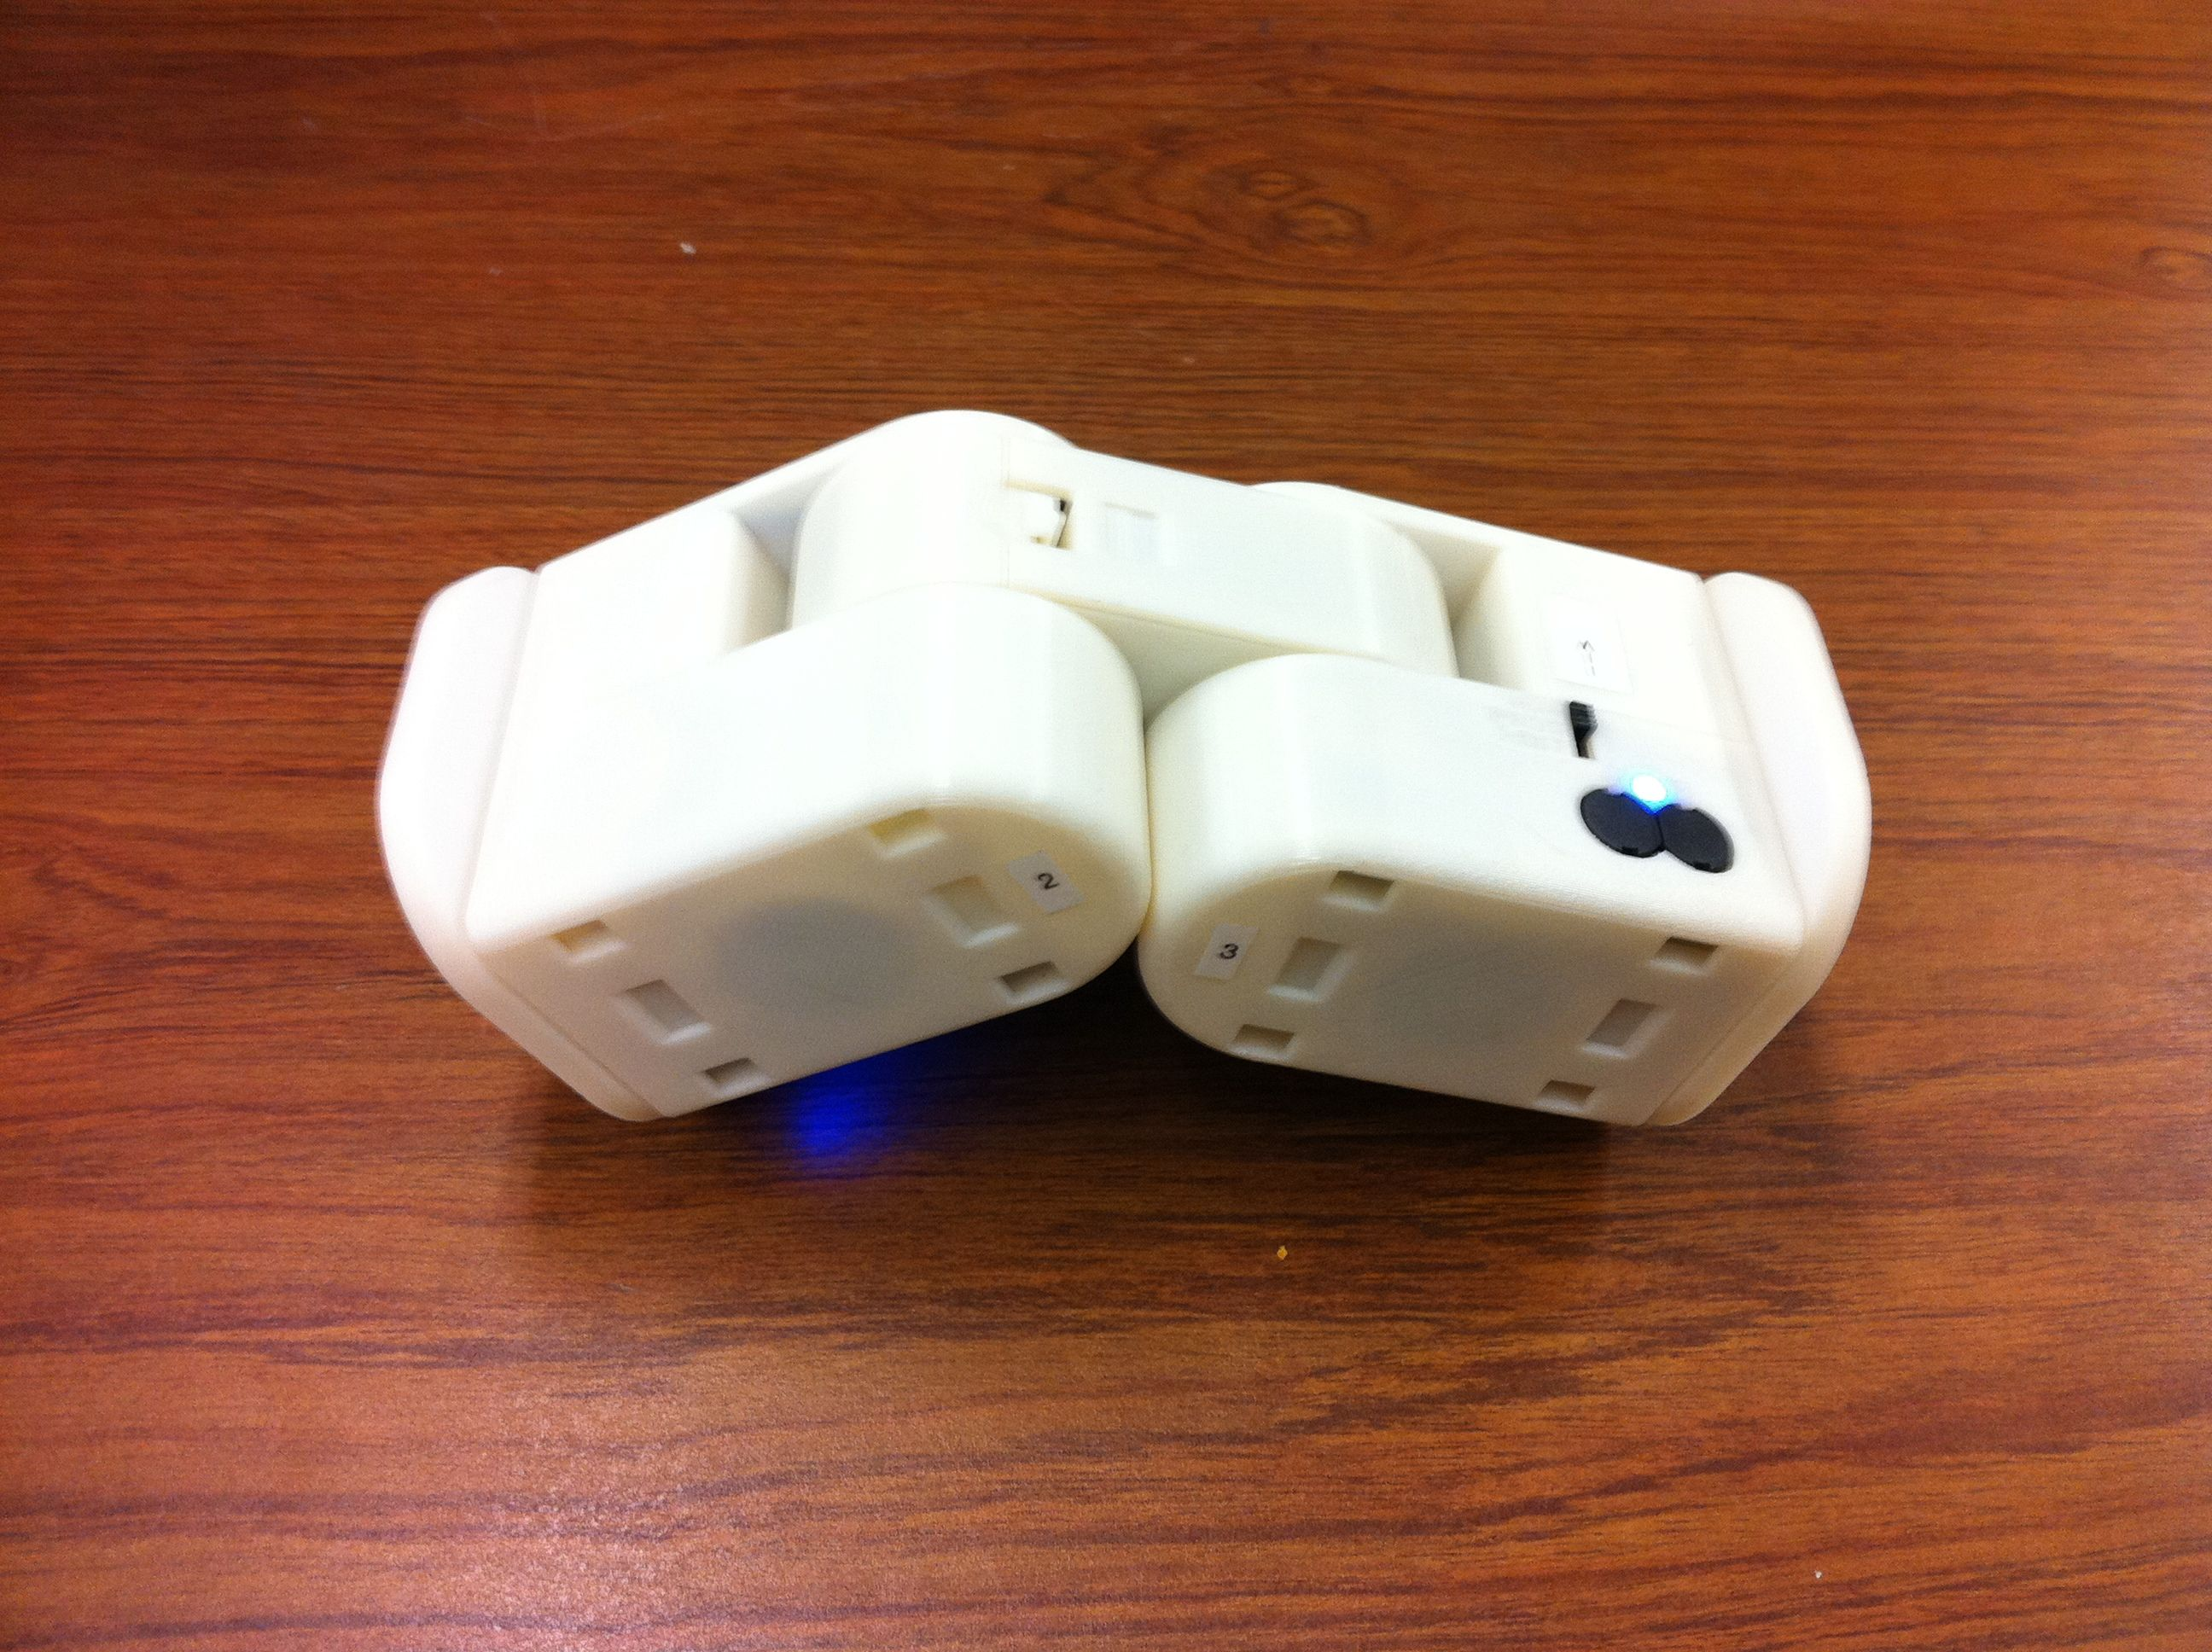
\includegraphics[width=1in]{images/inchworm2.jpg}}
  \subfloat[Move joint 3]{\label{fig:inchworm3}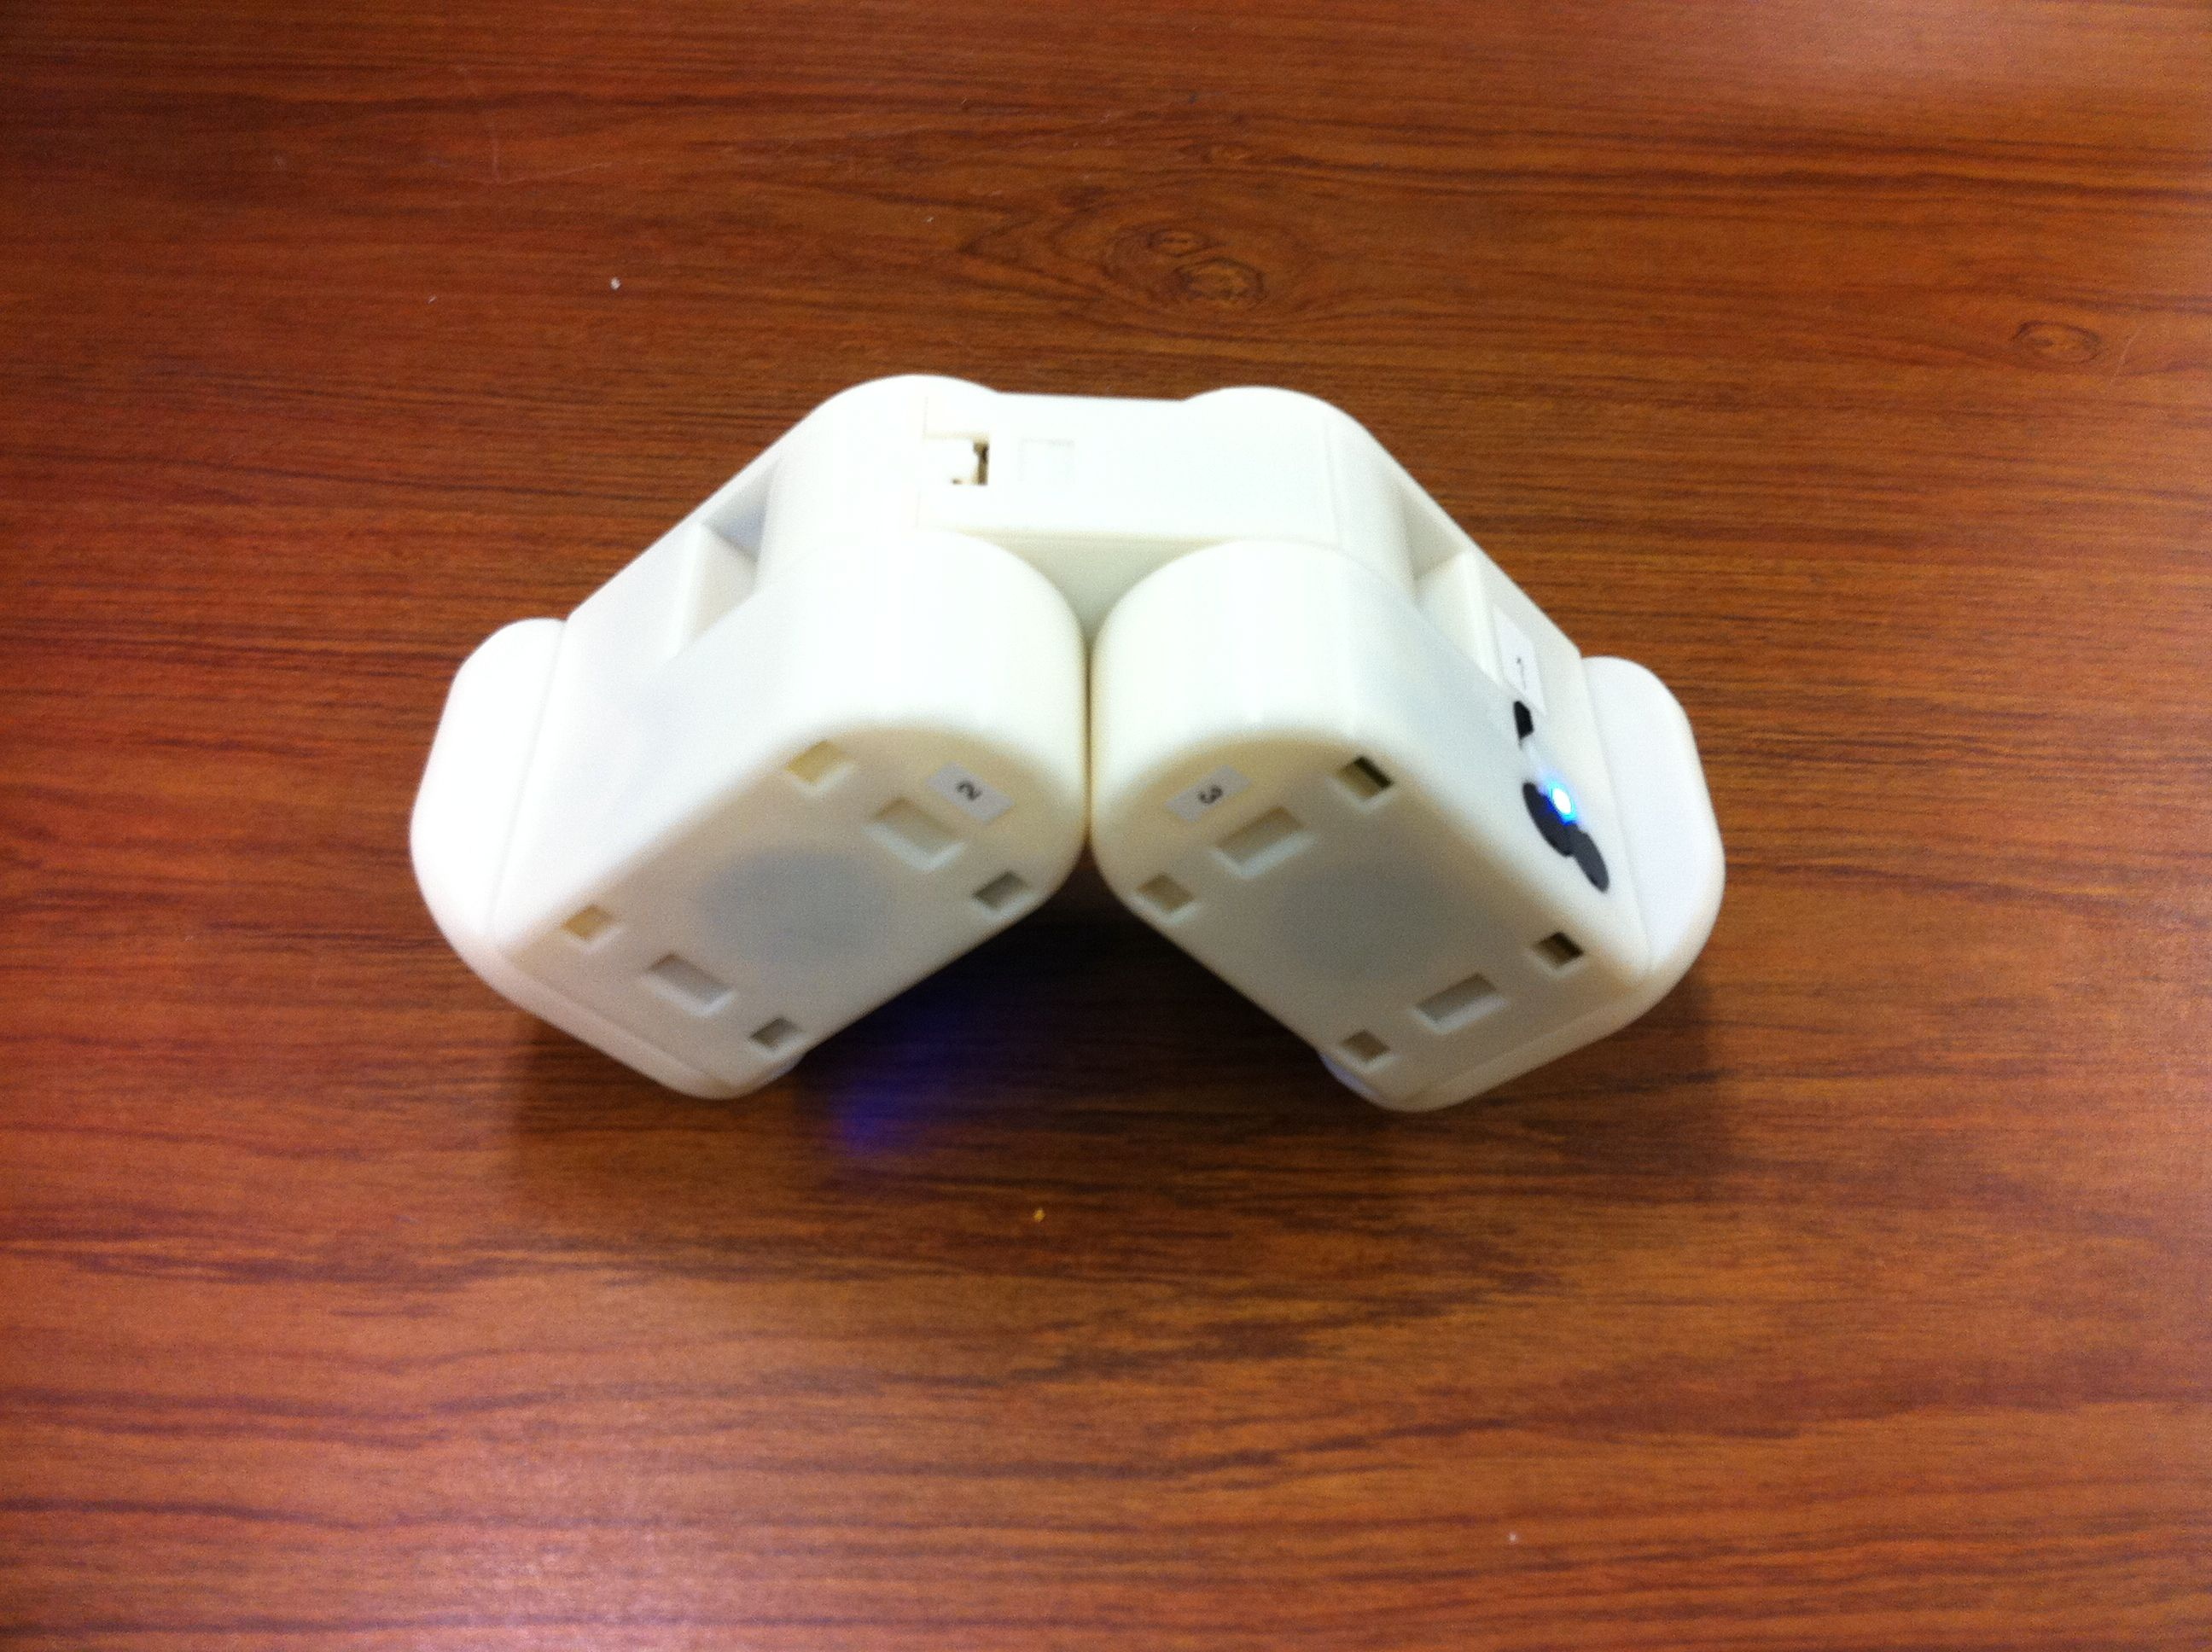
\includegraphics[width=1in]{images/inchworm4.jpg}}
  \subfloat[Move joint 2]{\label{fig:inchworm4}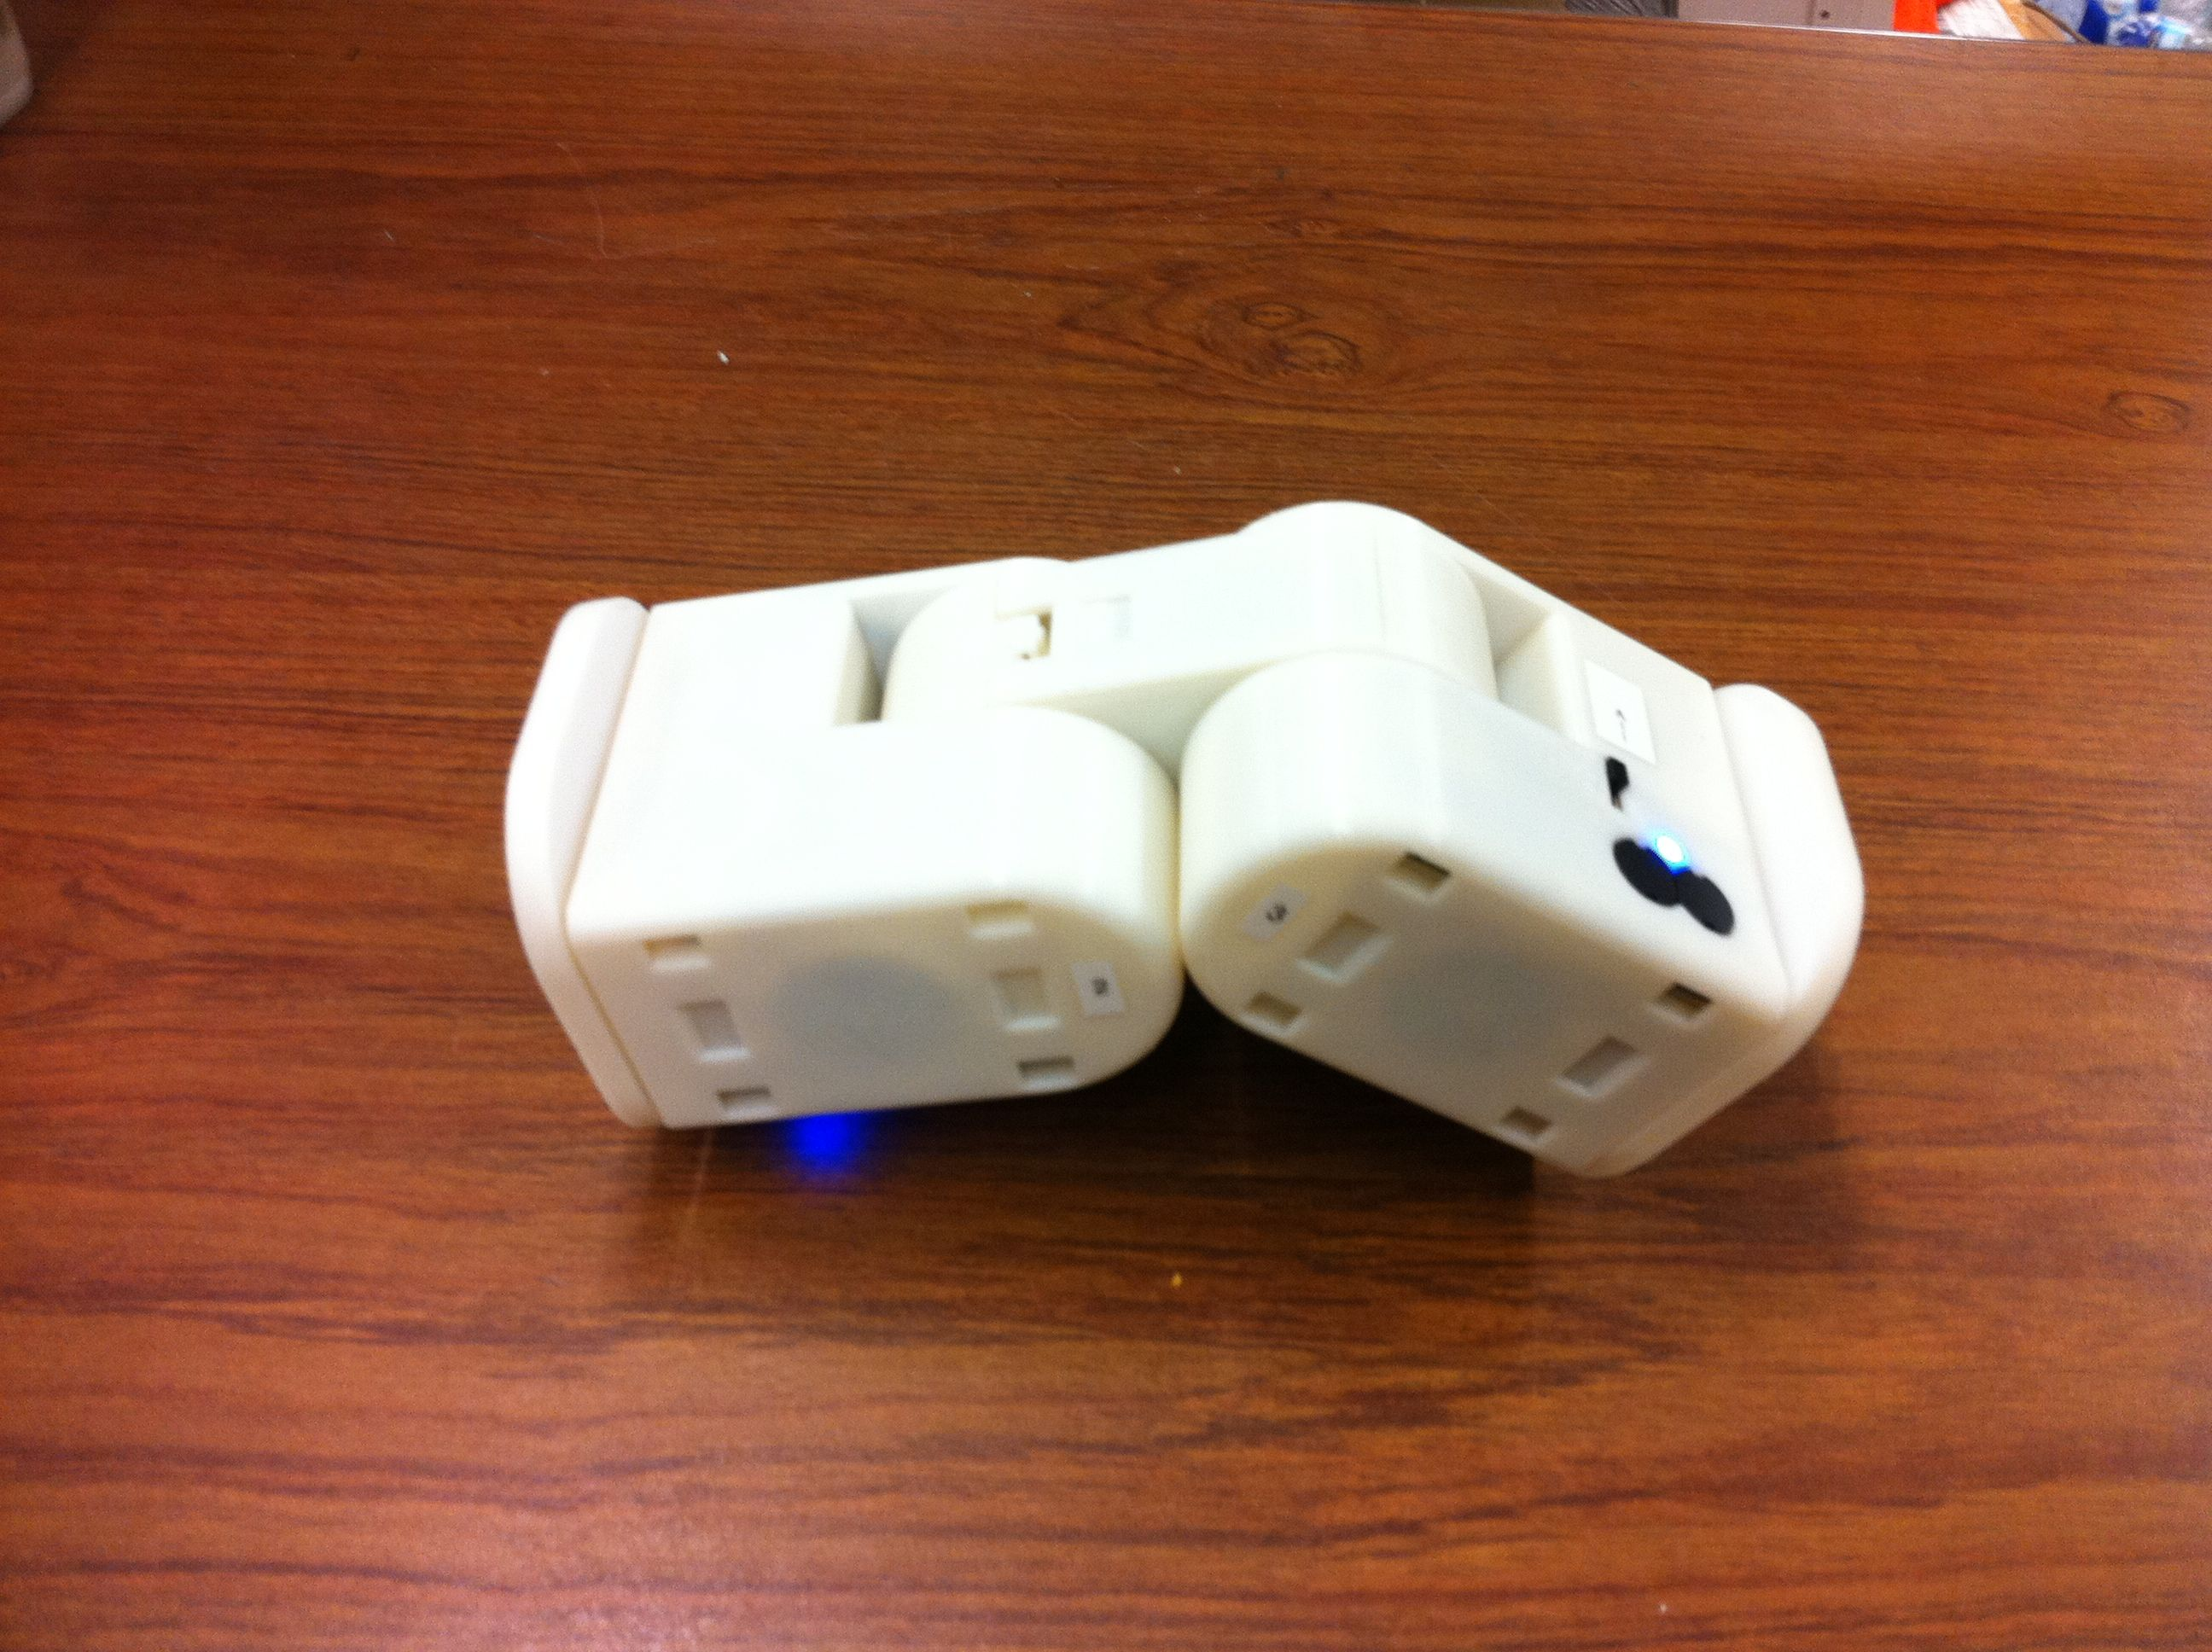
\includegraphics[width=1in]{images/inchworm3.jpg}}
  \subfloat[Move joint 3 back to zero position]{\label{fig:inchworm5}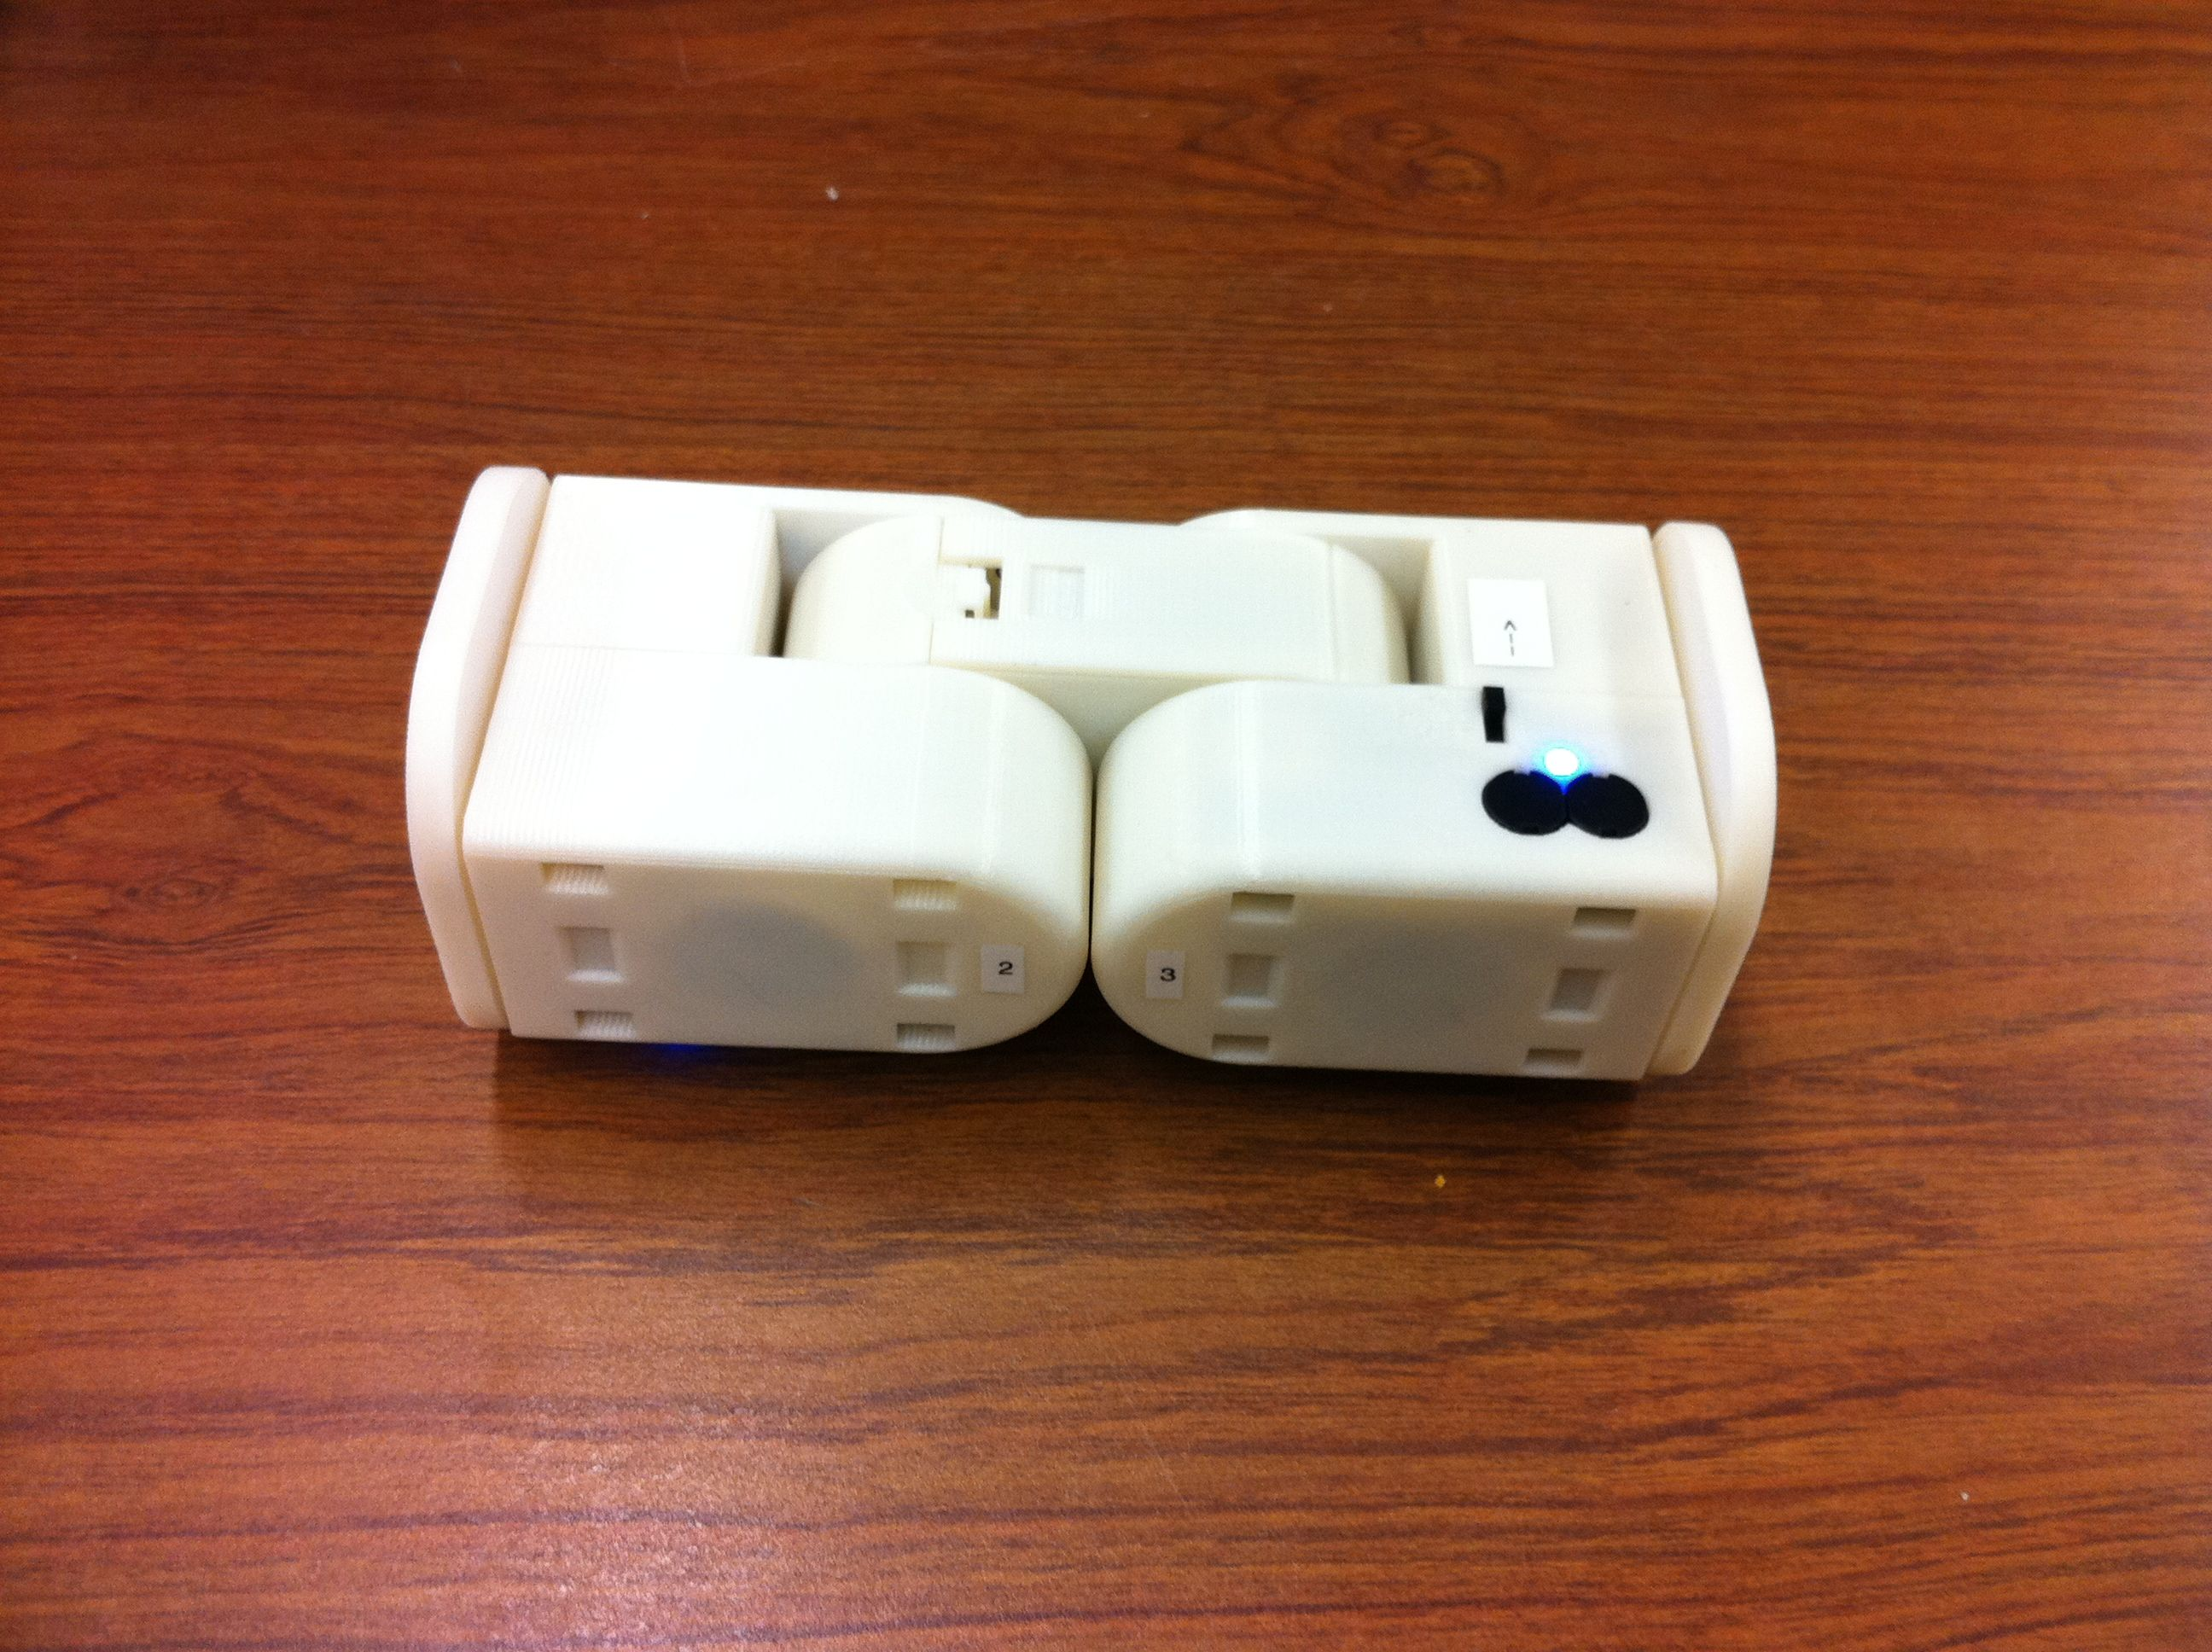
\includegraphics[width=1in]{images/inchworm1.jpg}}
  \caption{The inchworm motion}
  \label{fig:inchworm}
\end{figure}

Finally, we perform the actual inchworm motion. The inchworm motion is a gait defined
by a sequence of motions performed by the body joints. The motions are as such:
\begin{enumerate}
\item The first body joint, referred to as joint A, rotates towards the ground.
This drags the Mobot towards the direction of joint A. (Figure \ref{fig:inchworm2})
\item The other body joint, joint B, rotates towards the ground. Since the center
of gravity is currently positioned over joint A, this causes the trailing body 
joint to slide toward joint A. (Figure \ref{fig:inchworm3})
\item Joint A moves back to a flat position. (Figure \ref{fig:inchworm4})
\item Joint B moves back to a flat position. (Figure \ref{fig:inchworm5})
\item Repeat, if desired.
\end{enumerate}
The direction of travel depends on the selection of the initial body joint. In
the following code example, joint 2 is chosen as the initial body joint to move.
In this case, the Mobot will traverse towards joint 2. The entire motion is
encapsulated in a ``for'' loop which executes the entire motion four times.
\begin{verbatim}
/* Do the inchworm gait four times */
int i, num = 4;
double angle2 = -45;
double angle3 = 45;
for(i = 0; i < num; i++) {
    mobot.moveJointTo(MOBOT_JOINT2, angle2); /* Move joint 2 */
    mobot.moveJointTo(MOBOT_JOINT3, angle3); /* Move joint 3 */
    mobot.moveJointTo(MOBOT_JOINT2, 0);      /* Move joint 2 */
    mobot.moveJointTo(MOBOT_JOINT3, 0);      /* Move joint 3 bace to zero position*/
}
\end{verbatim}
The values of the variables \texttt{angle2} and \texttt{angle3} may also be modified
to produce different variations of the inchworm gait to accomodate different terrain
textures and ground surfaces.

\subsection{Standing Demo}
\subsubsection{\texttt{stand2.ch} Source Code}
\verbatiminput{../demos/chdemos/stand2.ch}
\subsubsection{\texttt{stand2.ch} Explained}
The first portion of the program performs the necessary setup and connecting,
similar to the previous demos. Similar to the previous inchworm demo, the
motor speeds are set to a speed of 90 degrees per second, and the function \texttt{moveToZero()} is
called to put the mobot into a flat position. Next, the following lines
are executed:
\begin{verbatim}
mobot.moveJointTo(MOBOT_JOINT2, -85);
mobot.moveJointTo(MOBOT_JOINT3, 70);
\end{verbatim}
These movement commands cause the Mobot to curl up into a fetal position with
both of its faceplates facing toward the ground. The next line, 

\begin{verbatim}
delay(1);
\end{verbatim}
causes the program to pause for one second before continuing. This allows the
mobot to settle down, in case it was still in motion from the last movement.

Next, the Mobot rotates one 
of the faceplates by 45 degrees. 
\begin{verbatim}
mobot.moveJointTo(MOBOT_JOINT1, 45);
\end{verbatim}
This endplate will eventually become the ``foot'' of the standing Mobot. Next,
the Mobot lifts itself into a standing position, balancing on its endplate.
\begin{verbatim}
mobot.moveJointTo(MOBOT_JOINT2, 20);
\end{verbatim}
Note that the previous joint angle for Joint 2, a body joint, was -85 degrees. 
This motion causes joint 2 to rotate all the way to a 20 degree position, which
lift up the body of the Mobot such that the Mobot is balancing on faceplate joint 1.

Finally, we rotate joint 1, the foot joint, for three seconds which causes the
entire Mobot to rotate in place. The speed is first set to 45 degrees per second to make the
rotation a slow rotation. Next, the \texttt{moveContinuousTime} member function
is used to continuously rotate a joint for a desired amount of time.
\begin{verbatim}
mobot.setJointSpeed(MOBOT_JOINT1, 45);
mobot.moveContinuousTime(MOBOT_FORWARD, MOBOT_HOLD, MOBOT_HOLD, MOBOT_HOLD, 3);
\end{verbatim}

\section{\label{sec:blocking}Blocking and Non-Blocking Functions}
All of the Mobot movement functions may be designated as either ``blocking'' 
functions or ``non-blocking'' functions. A blocking function is a function which
does not return while operations are being performed. All standard C functions,
such as \texttt{printf()}, are blocking functions. The
\texttt{moveWait()} function is a blocking function. When called, the function
will hang, or ``block'', until all the joints have stopped moving. After all
joints have stopped moving, the \texttt{moveWait()} function will return, and 
the rest of the program will execute.

Furthermore, some functions have both a blocking version and a non-blocking
version. For these functions, the suffix \texttt{NB} denotes that the function
is non-blocking. For instance, the function \texttt{motionStand()} is blocking,
meaning the function will not return until the motion is completed, whereas
the function \texttt{motionStandNB()} is non-blocking, meaning the function
returns immediately and the mobot performs the ``standing'' motion
asynchronously.

The function \texttt{moveNB()} is an example of a non-blocking function. When
the \texttt{moveNB()} function is called, the function immediately returns 
as the joints begin moving. Any lines of code following the call to 
\texttt{moveNB()} will be executed even if the current motion is still in
progress. 

Demos for the non-blocking functions are located in the next section of
this document.

\subsection{List of Blocking Movement Functions}
\begin{itemize}
\item \texttt{driveJointToDirect()}
\item \texttt{driveToDirect()}
\item \texttt{move()}
\item \texttt{moveContinuousTime()}
\item \texttt{moveJoint()}
\item \texttt{moveJointTo()}
\item \texttt{moveJointWait()}
\item \texttt{moveTo()}
\item \texttt{moveToZero()}
\item \texttt{moveWait()}
\item \texttt{motionArch()}
\item \texttt{motionInchwormLeft()}
\item \texttt{motionInchwormRight()}
\item \texttt{motionRollBackward()}
\item \texttt{motionRollForward()}
\item \texttt{motionSkinny()}
\item \texttt{motionStand()}
\item \texttt{motionTumbleLeft()}
\item \texttt{motionTumbleRight()}
\item \texttt{motionTurnLeft()}
\item \texttt{motionTurnRight()}
\item \texttt{motionUnstand()}
\end{itemize}

\subsection{List of Non-Blocking Movement Functions}
\begin{itemize}
\item \texttt{driveJointToDirectNB()}
\item \texttt{driveToDirectNB()}
\item \texttt{moveNB()}
\item \texttt{moveContinuousNB()}
\item \texttt{moveJointNB()}
\item \texttt{moveJointToNB()}
\item \texttt{moveToNB()}
\item \texttt{moveToZeroNB()}
\item \texttt{motionArchNB()}
\item \texttt{motionInchwormLeftNB()}
\item \texttt{motionInchwormRightNB()}
\item \texttt{motionRollBackwardNB()}
\item \texttt{motionRollForwardNB()}
\item \texttt{motionSkinnyNB()}
\item \texttt{motionStandNB()}
\item \texttt{motionTumbleLeftNB()}
\item \texttt{motionTumbleRightNB()}
\item \texttt{motionTurnLeftNB()}
\item \texttt{motionTurnRightNB()}
\item \texttt{motionUnstandNB()}
\end{itemize}

\subsection{Blocking and Non-Blocking Demo Programs}
\subsubsection{\texttt{nonblock.ch} Source Code}
\verbatiminput{../demos/chdemos/nonblock.ch}
\subsubsection{\texttt{nonblock.ch} Source Code Explanation}
This demo gives an example of how non blocking functions operate. 
After the initial setup and initialization similar to the previous
demos, the following line is executed:
\begin{verbatim}
mobot.moveNB(720, 0, 0, 720); // Non-Blocking version
\end{verbatim}
The function \texttt{moveNB()} is a non-blocking function, which means
that the program will continue executing even before the movement
has completed. The next lines of code appear as such:
\begin{verbatim}
while(mobot.isMoving()) {
    printf("mobot is moving ...\n");
}
\end{verbatim}
The previous lines of code basically loops as long as the \texttt{mobot.isMoving()} function
is returning true. In other words, in plain english, as long as the mobot is moving,
the program will print the message ``mobot is moving...''. As soon as the mobot completes
its motion, the loop will break and the message ``move finished!'' is printed.

Alternatively, there is a commented line of code that appears in the program, which
appears as
\begin{verbatim}
mobot.move(720, 0, 0, 720); // Non-Blocking version
\end{verbatim}
If the \texttt{moveNB()} function is replaced with the \texttt{move()} function in this program,
the message ``mobot is moving...'' is never printed to the screen. This is due to the
fact that \texttt{move()} is a blocking function, and by the time the program continues past
the \texttt{move()} statement, the mobot has already stopped moving.

\subsubsection{\texttt{nonblock2.ch} Source Code}
\verbatiminput{../demos/chdemos/nonblock2.ch}
\subsubsection{\texttt{nonblock2.ch} Source Code Explanation}
The first block of the source code initialized and sets up the remote mobot 
similar to previous demos. The last two lines in the program appear like so:
\begin{verbatim}
mobot.moveJointNB(MOBOT_JOINT1, 360); // Non-Blocking version
mobot.moveJoint(MOBOT_JOINT4, 360);
\end{verbatim}
The first line turns joint 1 for 360 degrees. However, since it is moved with a non-blocking function,
the program immediately continues to the next line. The second line turns joint 4 for
360 degrees. Because computer programs execute so fast compared to the physical
motion of the mobots, this program effectively begins rotating joints 1 and 4 
simultaneously. Since the function \texttt{moveJoint()} is a blocking function,
the program will not execute beyond that point until joint 4 has finished moving.

\subsubsection{\texttt{nonblock3.ch} Source Code}
\verbatiminput{../demos/chdemos/nonblock3.ch}
\subsubsection{\texttt{nonblock3.ch} Source Code Explanation}
The first section of code initializes the necessary variables to control remote
mobots as seen in previous demos. Next, we print a message on the screen and 
roll the mobot forward with the following two lines of code.
\begin{verbatim}
printf("Rolling 360 degrees.\n");
mobot.motionRollForward(360);
\end{verbatim}
Next, we make two calls to non-blocking functions.
\begin{verbatim}
mobot.motionArchNB(15);
mobot.motionRollForwardNB(360);
\end{verbatim}
The first call is to the function \texttt{motionArchNB()}, which arches the mobot
up by moving joints 2 and 3. Since it is a non-blocking function, the program
immediately continues on even before the arching motion as finished. The
next call rolls the mobot forward by rotating joints 1 and 4. In effect, these
two lines cause the mobot to roll forward and arch simultaneously. It is important
to note that this compound motion works because the Arch motion only moves 
joints 2 and 3 while the rolling motions only move joints 1 and 4, so there are
no conflicting motor commands.

In order to wait for all motions to finish, the last line of the program is
\begin{verbatim}
mobot.motionWait();
\end{verbatim}
The \texttt{motionWait()} function will wait until all mobot motions are finished.

Note that
if a program contains non-blocking functions, it is typically necessary to 
call a waiting function such as \texttt{moveWait()} or \texttt{motionWait()}
before the program terminates. If a waiting function is not called, the program
may terminate before the motion has been completed, which may halt the mobot
in the middle of one of its motions.

\subsection{Preprogrammed Motion Demos with Non-Blocking Functions}
\subsubsection{\texttt{unstand2.ch} Source Code}
\verbatiminput{../demos/chdemos/unstand2.ch}
\subsubsection{\texttt{unstand2.ch} Source Code Explanation}
The first block of code,
\begin{verbatim}
/* Filename: unstand.ch 
 * Drop the mobot down from a standing position. */
#include <mobot.h>
CMobot mobot;

/* Connect to the paired Mobot */
mobot.connect();
\end{verbatim}
initialize the program and connect to the remote mobot. Next, a series of
non-blocking movements are performed:
\begin{verbatim}
mobot.moveJointToNB(MOBOT_JOINT2, -85);
mobot.moveJointToNB(MOBOT_JOINT3, 45);
\end{verbatim}
Because both of these function calls are non-blocking, this function will
effectively move joints 2 and 3 simultaneously. Since these are both
non-blocking functions, a call to \texttt{moveWait()} is necessary to
wait for the mobot to complete its motions, as done in the next line:
\begin{verbatim}
mobot.moveWait();
\end{verbatim}

Finally, we move the mobot into a flat zero position with the following line:
\begin{verbatim}
mobot.moveToZero();
\end{verbatim}

\subsubsection{\texttt{tumble2.ch} Source Code}
\verbatiminput{../demos/chdemos/tumble2.ch}
\subsubsection{\texttt{tumble2.ch} Source Code Explanation}
The first lines of the program,
\begin{verbatim}
#include <mobot.h>
CMobot mobot;

/* Connect to the paired Mobot */
mobot.connect();

/* Set the mobot to "home" position, where all joint angles are 0 degrees. */
mobot.moveToZero();
\end{verbatim}
initialize the proper variables and connections as seen in previous demos.

Next, we begin the tumbling motion. We consider each tumbling motion to be the 
mobot flipping over twice. The reason the mobot flips twice per tumble is so that
when the tumbling motion is done, the mobot ends right side up. 
A for loop is used to to tumble ``num'' times, as shown in the following code:
\begin{verbatim}
int i, num = 2;
for(i = 0; i < num; i++) {
\end{verbatim}
These lines create two new variables, ``i'' and ``num'', which are the loop
counter, and the number of times to tumble, respectively. 

Inside the loop, two tumbling motions are performed. The first tumbling
motion appears as such:
\begin{verbatim}
    /* First lift and tumble */
    mobot.moveJointTo(MOBOT_JOINT2, -85);
    mobot.moveJointTo(MOBOT_JOINT3, 80);
    mobot.moveJointTo(MOBOT_JOINT2, 0);
    mobot.moveJointTo(MOBOT_JOINT3, 0);
    mobot.moveJointTo(MOBOT_JOINT2, 80);
    mobot.moveJointTo(MOBOT_JOINT2, 45);
\end{verbatim}
This movement is similar to the \texttt{motionStand()} motion, except that the
mobot flips all the way over after standing up. After this motion is done,
the mobot is balancing on joint 4. Next, we flip again so that the mobot
is balancing on joint 1.
\begin{verbatim}
    /* Second lift and tumble */
    mobot.moveJointTo(MOBOT_JOINT3, -85);
    mobot.moveJointTo(MOBOT_JOINT2, 80);
    mobot.moveJointTo(MOBOT_JOINT3, 0);
    mobot.moveJointTo(MOBOT_JOINT2, 0);
    mobot.moveJointTo(MOBOT_JOINT3, 80);
    if(i != (num-1)) { /* Do not perform this motion on the last tumble */
        mobot.moveJointTo(MOBOT_JOINT3, 45);
    }
}
\end{verbatim}
The \texttt{if} statement prevents the last motion from being executed
when the mobot is on its last tumble. This is because the last motion in the
loop is a prepatory motion for the next tumble, which is not needed if the
mobot is currently performing its last tumble. 

The entire motion, consisting of two flips, are performed ``num'' times. After
the loop is completed, the mobot is made to fall back down into a prone
positions with the following lines of code:
\begin{verbatim}
/* Unstand the mobot */
mobot.moveJointToNB(MOBOT_JOINT2, 0);
mobot.moveJointToNB(MOBOT_JOINT3, 0);
mobot.moveWait();
mobot.moveToZero();
\end{verbatim}


\section{Controlling Multiple Modules}
The Mobot control software is designed to be able to control multiple modules
simultaneously. There are some important differences in the program 
which enable the control of multiple modules. A small demo program which
controls two modules simultaneously will first be presented, followed by
a detailed explanation of the program elements.

\subsection{\texttt{twoModules.ch} Source Code}
\verbatiminput{../demos/chdemos/twoModules.ch}

\subsection{Demo Explanation}
The first two lines of interest appear as such:
\begin{verbatim}
  CMobot mobot1;
  CMobot mobot2;
\end{verbatim}
These two lines declare two separate variables which will represent the
two separate Mobot modules. Next, we need to connect each variable to
a physically separate Mobot. This is done with the following lines.
\begin{verbatim}
  mobot1.connect();
  mobot2.connect();
\end{verbatim}
These two lines connect the mobots to the first two addresses
of the known mobot addresses. The list of the computer's known
mobot addresses may be configured in the process detailed in Section
\ref{sec:pairing} on page \pageref{sec:pairing}. For each separate
control program, the first call to the \texttt{connect()} member
function will connect to the first mobot listed in the configuration
file. Each successive call to the \texttt{connect()} function will
connect to successive mobots listed in the configuration file. 
The order in which they are connected may be modified using the
``Configure Mobot Bluetooth'' dialog, as discussed in Section
\ref{sec:pairing}.

\begin{verbatim}
  mobot1.moveToZeroNB();
  mobot2.moveToZeroNB();
\end{verbatim}
These two lines command the two mobots to move to their zero positions.
Note that these functions are non-blocking. This means that the
\texttt{moveToZeroNB()} function will return immediately, and will not
wait for the first mobot to finish completing the motion before 
commanding the second mobot to begin. In a normal program, this effectively
causes both mobots to move to their zero positions simultaneously.

\begin{verbatim}
  mobot1.moveWait();
  mobot2.moveWait();
\end{verbatim}
Since the \texttt{moveToZeroNB()} functions are non-blocking, we would like
the program to wait until the motions are complete before continuing. By
calling \texttt{moveWait()} on both of the mobots, we can be assured that
the mobots have finished moving before the program continues.

\begin{verbatim}
  mobot1.motionStandNB();
  mobot2.motionInchwormLeftNB(4);
\end{verbatim}
Similar to the calls to \texttt{moveToZeroNB()}, this block of code instructs 
the first Mobot to stand and the second Mobot to perform the inchworm motion four times.
Note that we call the non-blocking versions of the
functions, \texttt{motionStandNB()} and \texttt{motionInchwormLeftNB()}. Since these functions are
non-blocking, both mobots will effectively perform the motions simultaneously. 

When the first mobot finishes standing, we want it to spin around on its faceplate
while the second mobot is still inchworming. We can accomplish this by first
waiting for the standing motion to finish, and then moving the faceplate joints
of the first mobot, as in the following lines of code.
\begin{verbatim}
  mobot1.motionWait();
  mobot1.moveNB(360, 0, 0, 360);
\end{verbatim}

Before we continue with the program, we wish to ensure that motion has stopped on both
mobots. Since the the last command sent to \texttt{mobot1} was a \texttt{moveNB()}
command, we use the \texttt{moveWait()} function to wait for that movement to finish.
Similarly, the last command sent to \texttt{mobot2} was a motion command, and so we
use \texttt{motionWait()} to wait for the motion to finish. The two lines of code
are seen in the program as follows:
\begin{verbatim}
  mobot1.moveWait();
  mobot2.motionWait();
\end{verbatim}

Finally, the following lines,
\begin{verbatim}
mobot1.motionUnstandNB();
mobot2.motionInchwormRightNB(4);
mobot1.motionWait();
mobot1.motionTumbleLeft(1);
mobot2.motionWait();
\end{verbatim}
make the first mobot come back down from its standing position and the second mobot
inchworm to the right four times simultaneously. Note that the function 
\texttt{motionWait()} is used to wait for motions, which are compound
movements, to finish. This is similar to how
the function \texttt{moveWait()} is used to wait for individual movements
to finish. After \texttt{mobot1} finishes unstanding, it will begin 
a tumbling motion. Since the tumbling motion function is called before the call
to \texttt{mobot2.motionWait()}, \texttt{mobot1} will begin tumbling even if
\texttt{mobot2} has finished its previous motion, which was inchworming 4 times.

\subsection{Controlling Multiple Connected Modules}
\subsubsection{\texttt{lift.ch}, Lifting Demo}
\verbatiminput{../demos/chdemos/lift.ch}
\subsubsection{\texttt{lift.ch} Source Code Explanation}
This demo is designed to lift two connected modules up into
a two-legged standing configuration. The mobots are connected such that the fourth
joint of mobot one is connected to the first joint of mobot two. The two connect mobots
act as one long mobot.

The first portion of the program initialize two variables called \texttt{mobot1} 
and \texttt{mobot2}, which will be used to control the two connected modules.
Once the mobots are initialized, they are both moved into a flat zero position.

The next lines,
\begin{verbatim}
/* First lift */
mobot1.moveNB(0, -90,  0, 0);
mobot2.moveNB(0, 0, 90, 0);
mobot1.moveWait();
mobot2.moveWait();
\end{verbatim}
rotate the joints on either end of the compound mobot to perform the 
first portion of the lift, as shown in Figure \ref{fig:lift1}. The motion is performed as two non-blocking
calls to \texttt{moveNB()} and then waiting for both movements to finish.

\begin{figure}
  \centering
  \subfloat[First lift]{\label{fig:lift1}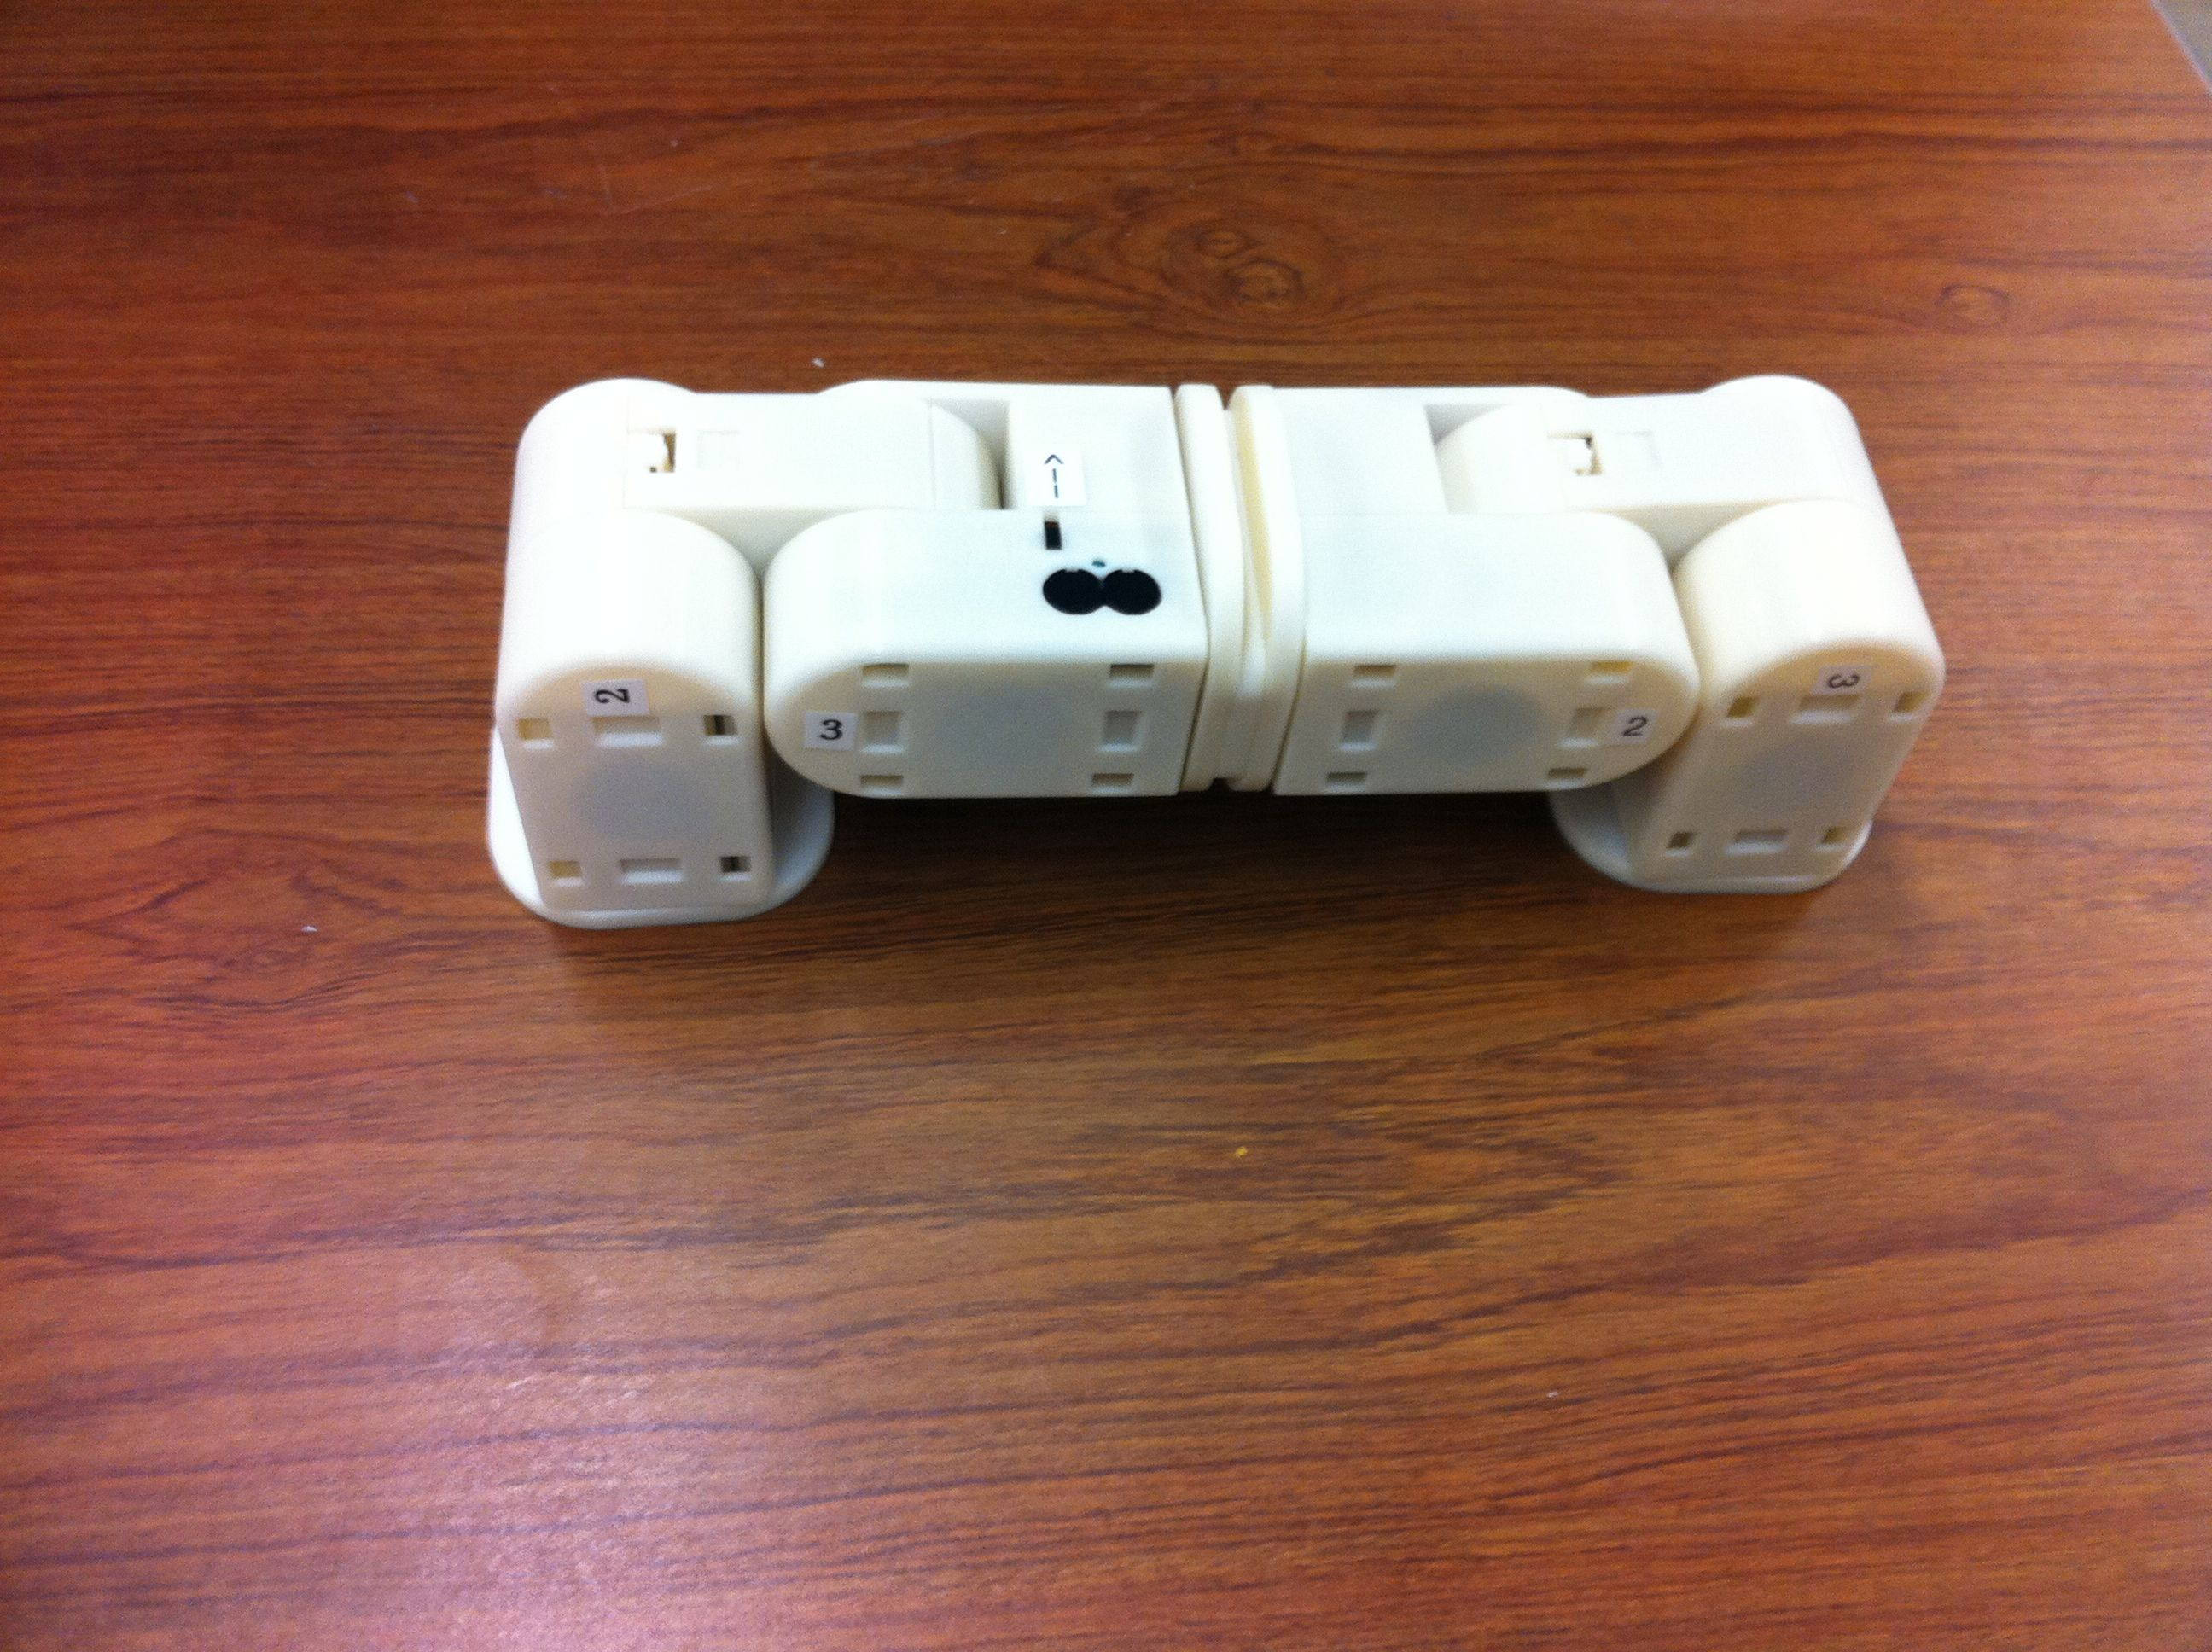
\includegraphics[width=2in]{images/lift1_v2.jpg}}
  \subfloat[Second lift]{\label{fig:lift2}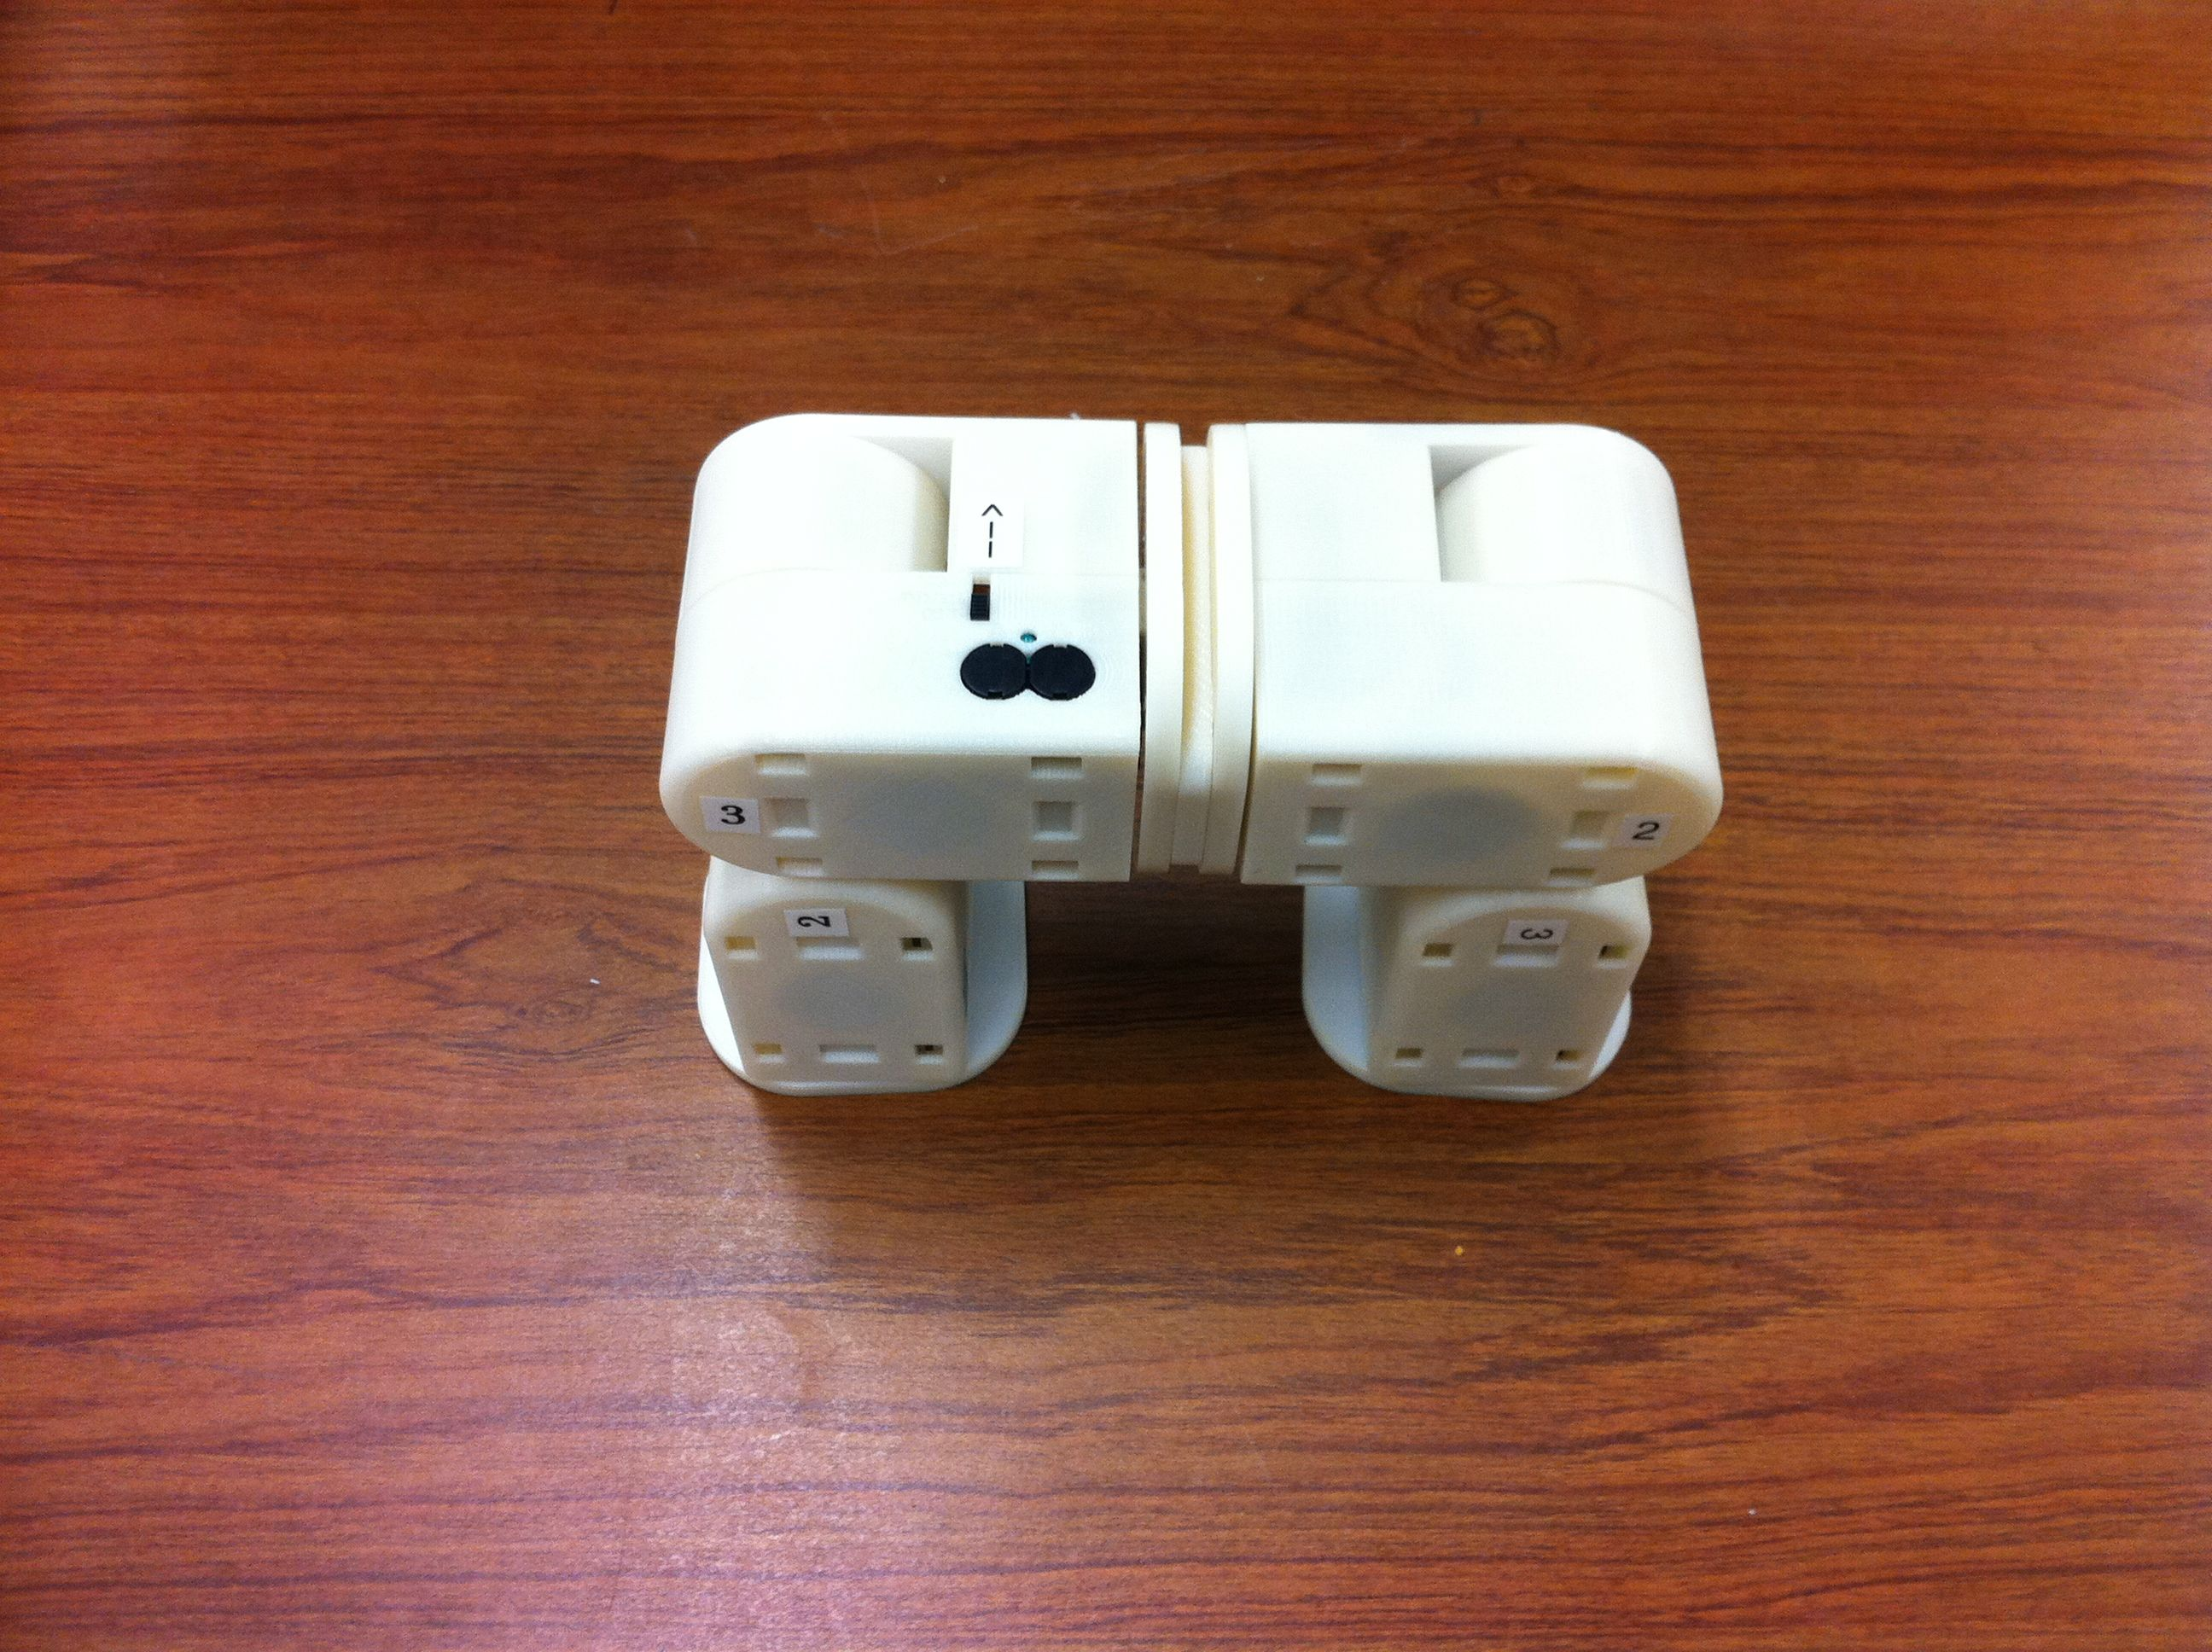
\includegraphics[width=2in]{images/lift2_v2.jpg}}
  \caption{Lifting motion with two connected modules}
  \label{fig:lift}
\end{figure}

The next lines rotate the inner joints of the compound mobot to lift the mobot
one step higher, as shown is Figure \ref{fig:lift2}.
\begin{verbatim}
/* Second lift */
mobot1.moveToNB(0, 0, 90,  0);
mobot2.moveToNB(0,  -90, 0, 0);
mobot1.moveWait();
mobot2.moveWait();
\end{verbatim}
Again, these lines perform two calls to the non-blocking function
\texttt{moveNB()} and then wait for the movements to finish.

Finally, we move both mobots back to their zero positions, which drops 
the compound mobot back onto the ground.
\begin{verbatim}
mobot1.moveToZeroNB();
mobot2.moveToZeroNB();
mobot1.moveWait();
mobot2.moveWait();
\end{verbatim}

\section{Commanding Multiple Mobots to Perform Identical Tasks}
The class called \texttt{CMobotGroup} can be used
to control multiple modules simultaneously. The \texttt{CMobotGroup} represents
a group of mobots. Any command that is given to the group of modules is 
duplicated to each member of the group.

The majority of the movement functions available in the \texttt{CMobot} class
are also available in the \texttt{CMobotGroup} class. 
The detailed information for each member function are presented in 
Appendix \ref{sec:cmobotgroup_api}.
 Following
is a complete listing of the available member functions in the \texttt{CMobotGroup}
class.

\vspace{8pt}
\noindent
\begin{tabular}{p{1.75in}p{4.5in}}
%\begin{tabular}{ll}
\hline
Function & Description \\
\hline
%\texttt{pose()} \dotfill & Pose multiple joints of the mobot. \\
\texttt{CMobotGroup()} & The CMobotGroup constructor function. This function
is called automatically and should not be called explicitly. \\
\texttt{\textasciitilde CMobotGroup()} & The CMobotGroup destructor function. This function
is called automatically and should not be called explicitly. \\
& \\
\texttt{addRobot()} & Add a mobot to be a member of the mobot group. \\
\texttt{move()} & Move all four joints of the mobots by specified angles. \\
\texttt{moveNB()} & Identical to \texttt{move()} but non-blocking. \\
\texttt{moveContinuousNB()} & Move joints continuously. Joints will move untill stopped.\\
\texttt{moveContinuousTime()} & Move joints continuously for a certain amount of time.\\
\texttt{moveJointContinuousNB()} & Move a single joint on all mobots continuously. \\
\texttt{moveJointContinuousTime()} & Move a single joint on all mobots continuously for a specific amount of time. \\
\texttt{moveJoint()} & Move a motor from its current position by an angle. \\
\texttt{moveJointNB()} & Identical to \texttt{moveJoint()} but non-blocking. \\
\texttt{moveJointTo()} & Set the desired motor position for a joint. \\
\texttt{moveJointToNB()} & Identical to \texttt{moveJointTo()} but non-blocking. \\
\texttt{moveJointWait()} & Wait until the specified motor has stopped moving. \\
\texttt{moveTo()} & Move all four joints of the mobots to specified absolute angles. \\
\texttt{moveToNB()} & Identical to \texttt{moveTo()} but non-blocking. \\
\texttt{moveToZero()} & Instructs all motors to go to their zero positions. \\
\texttt{moveToZeroNB()} & Identical to \texttt{moveToZero()} but non-blocking. \\
\texttt{moveWait()} & Wait until all motors have stopped moving. \\
%\texttt{setJointDirection()} & Set the motor direction of a motor. Set
%to "0" for automatic direction, "1" for forward, and "2" for reverse. \\
\texttt{setJointSpeed()} & Set a motor's speed setting in radians per second. \\
\texttt{setJointSpeeds()} & Set all motor speeds in radians per second. \\
\texttt{setJointSpeedRatio()} & Set a joints speed setting to a fraction of its maximum speed, a value between 0 and 1. \\
\texttt{setJointSpeedRatios()} & Set all joint speed settings to a fraction of its
maximum speed, expressed as a value from 0 to 1. \\
\texttt{setTwoWheelRobotSpeed()} & Move the mobots at a constant forward velocity. \\
\texttt{stop()} & Stop all currently executing motions of the mobot. \\
\hline
\end{tabular}

\begin{comment}
\begin{tabular}{p{1.75in}p{4.5in}} \hline 
Function Name & Description \\
\hline
\texttt{addRobot()} & Add a mobot to the group. \\
\texttt{move()} & Move joints on mobots from their current positions for all mobots in the group. \\
\texttt{moveContinuousNB()} & Move joints continuously for all mobots in the group. \\
\texttt{moveContinunousTime()} & Move joints continuously for a specific amount of time for all mobots in the group.\\
\texttt{moveJointContinuousNB()} & Move a single joint continuously for all mobots in the group. \\
\texttt{moveJointContinuousTime()} & Move a single joint continuously for a specific amount of time for all mobots in the group.\\
\texttt{moveJointTo()} & Move a joint to an absolute angle for all mobots in the group.\\
\texttt{moveJointWait()} & Wait for a joint to finish moving for all mobots in the group. \\
\texttt{moveTo()} & Move joints to a set of specific angles for all mobots in the group. \\
\texttt{moveWait()} & Wait for all joints to finish moving. \\
\texttt{moveToZero()} & Move all joints to their zero positions. \\
\texttt{setJointSpeed()} & Set the speed of a joint, in radians per second. \\
\texttt{setJointSpeedRatio()} & Set the speed of a joint as a ratio of the maximum speed. \\
\texttt{setTwoWheelRobotSpeed()} & Move the mobot at a linear speed, given the wheel size and desired speed.\\
\texttt{stop()} & Stop all the joints of all mobots in the group. \\
\texttt{motionArch()} & Cause all mobots in the group to arch for higher rolling clearance. \\
\texttt{motionArchNB()} & Cause all mobots in the group to arch for higher rolling clearance. \\
\texttt{motionInchwormLeft()} & Cause all mobots in the group to inchworm. \\
\texttt{motionInchwormLeftNB()} & Cause all mobots in the group to inchworm. \\
\texttt{motionInchwormRight()} & Cause all mobots in the group to inchworm. \\
\texttt{motionInchwormRightNB()} & Cause all mobots in the group to inchworm. \\
\texttt{motionRollBackward()} & Makes all mobots in the group roll backward. \\
\texttt{motionRollForwardNB()} & Makes all mobots in the group roll forward. \\
\texttt{motionSkinny()} & Make all mobots in the group assume a skinny rolling profile. \\
\texttt{motionSkinnyNB()} & Make all mobots in the group assume a skinny rolling profile. \\
\texttt{motionStand()} & Make all mobots in the group stand. \\
\texttt{motionStandNB()} & Make all mobots in the group stand. \\
\texttt{motionTumbleLeft()} & Make all the mobots in the group perform the tumbling motion. \\
\texttt{motionTumbleLeftNB()} & Make all the mobots in the group perform the tumbling motion. \\
\texttt{motionTumbleRight()} & Make all the mobots in the group perform the tumbling motion. \\
\texttt{motionTumbleRightNB()} & Make all the mobots in the group perform the tumbling motion. \\
\texttt{motionTurnLeft()} & Make all mobots in the group turn left. \\
\texttt{motionTurnLeftNB()} & Make all mobots in the group turn left. \\
\texttt{motionTurnRight()} & Make all mobots in the group turn right. \\
\texttt{motionTurnRightNB()} & Make all mobots in the group turn right.\\
\texttt{motionUnstand()} & Make all mobots in the group drop down from a standing position. \\
\texttt{motionUnstandNB()} & Make all mobots in the group drop down from a standing position. \\
\texttt{motionWait()} & Wait for the mobots to complete all currently executing compound motions.\\
\hline
\end{tabular}
\end{comment}


\noindent
\begin{tabular}{p{1.75in}p{4.5in}}
Compound Motions & These are convenience functions of commonly used compound motions. \\
\hline
\texttt{motionArch()}  & Move each robot in the group into an arched configuration. \\
\texttt{motionArchNB()}  & Identical to \texttt{motionArch()} but non-blocking. \\
\texttt{motionInchwormLeft()}  & Inchworm motion towards the left. \\
\texttt{motionInchwormLeftNB()}  & Identical to \texttt{motionInchwormLeft()} but non-blocking. \\
\texttt{motionInchwormRight()}  & Inchworm motion towards the right. \\
\texttt{motionInchwormRightNB()}  & Identical to \texttt{motionInchwormRight()} but non-blocking. \\
\texttt{motionRollBackward()}  & Roll on the faceplates toward the backward direction. \\
\texttt{motionRollBackwardNB()}  & Identical to \texttt{motionRollBackward()} but non-blocking. \\
\texttt{motionRollForward()}  & Roll on the faceplates forwards. \\
\texttt{motionRollForwardNB()}  & Identical to \texttt{motionRollForward()} but non-blocking. \\
\texttt{motionSkinny()}  & Move the robots into a skinny configuration. \\
\texttt{motionSkinnyNB()}  & Identical to \texttt{motionSkinnyNB()} but non-blocking. \\
\texttt{motionStand()}  & Stand the robots up on its end. \\
\texttt{motionStandNB()}  & Identical to \texttt{motionStandNB()} but non-blocking. \\
\texttt{motionTumbleLeft()}  & Tumble the robots end over end. \\
\texttt{motionTumbleLeftNB()}  & Identical to \texttt{motionTumbleLeftNB()} but non-blocking. \\
\texttt{motionTumbleRight()}  & Tumble the robots end over end. \\
\texttt{motionTumbleRightNB()}  & Identical to \texttt{motionTumbleRightNB()} but non-blocking. \\
\texttt{motionTurnLeft()}  & Rotate the robots counterclockwise. \\
\texttt{motionTurnLeftNB()}  & Identical to \texttt{motionTurnLeft()} but non-blocking. \\
\texttt{motionTurnRight()}  & Rotate the robots clockwise. \\
\texttt{motionTurnRightNB()}  & Identical to \texttt{motionTurnRight()} but non-blocking. \\
\texttt{motionUnstand()}  & Move each robot in the group currently standing on its end down into zero position. \\
\texttt{motionUnstandNB()}  & Identical to \texttt{motionUnstand()} but non-blocking. \\
\texttt{motionWait()}  & Wait for preprogrammed robotic motions to complete. \\
\hline
\end{tabular}


\subsection{Demo program \texttt{group.ch}}
\subsubsection{Source Code}
\verbatiminput{../demos/chdemos/group.ch}

\subsubsection{Demo Explanation}
The first lines of interest appear as such:

\begin{verbatim}
CMobot mobot1;
CMobot mobot2;
CMobotGroup group;
\end{verbatim}

These lines declare two mobot variables, and one variable which
will represent a group of mobots. Next, we connect the mobot
variables to their physical counterparts.

\begin{verbatim}
mobot1.connect();
mobot2.connect();
\end{verbatim}

Once they are connected, we wish to add both of these mobots to our mobot group,
which we have named \texttt{group}.

\begin{verbatim}
group.addRobot(mobot1);
group.addRobot(mobot2);
\end{verbatim}

Finally, we wish for all of the mobots in our mobot group, namely
\texttt{mobot1} and \texttt{mobot2}, to peform an inchworm motion four times, followed
by a standing motion. This is done with the following lines:

\begin{verbatim}
group.motionInchwormLeft(4);  /* Both mobots inchworm left 4 times */
group.motionStand();          /* Both mobots stand */
\end{verbatim}

After the mobots stand up, the line
\begin{verbatim}
group.move(360, 0, 0, 360);   /* Joints 1 and 4 rotate 360 degrees */
\end{verbatim}
makes the mobots perform a 360 degree rotation on their faceplates
while standing.

The next line, 
\begin{verbatim}
delay(3);                     /* Mobots stand still for 3 seconds */
\end{verbatim}
makes the mobots stand still for three seconds. After standing
still for three seconds, the line
\begin{verbatim}
group.motionUnstand();        /* Mobots get back down from standing */
\end{verbatim}
makes both mobots move back down from a standing position into a prone
position.

\subsection{Demo Program \texttt{groups.ch}}
\subsubsection{\texttt{groups.ch} Source Code}
\verbatiminput{../demos/chdemos/groups.ch}
\subsubsection{Demo Explanation}
The program begins by including the \texttt{mobot.h} header file
and declaring a number of mobot variables and mobot group variables.
\begin{verbatim}
#include <mobot.h>
CMobot mobot1;
CMobot mobot2;
CMobot mobot3;
CMobot mobot4;
CMobotGroup groupA;
CMobotGroup groupB;
CMobotGroup groupC;
CMobotGroup groupD;
\end{verbatim}

Next, we connect our four robot variables to the first four robots 
configured in RoboMancer.
\begin{verbatim}
mobot1.connect();
mobot2.connect();
mobot3.connect();
mobot4.connect();
\end{verbatim}

Now we begin adding our mobots to their groups. We will have four different groups, and each mobot
will belong to more than one group. They will be organized as such:
\begin{itemize}
\item Group A: mobot1, mobot2, mobot3, mobot4
\item Group B: mobot1, mobot2
\item Group C: mobot3, mobot4
\item Group D: mobot1, mobot2, mobot3
\end{itemize}
The following code divides the mobots up into our groups.
\begin{verbatim}
/* Group A */
groupA.addRobot(mobot1);
groupA.addRobot(mobot2);
groupA.addRobot(mobot3);
groupA.addRobot(mobot4);

/* Group B */
groupB.addRobot(mobot1);
groupB.addRobot(mobot2);

/* Group C */
groupC.addRobot(mobot3);
groupC.addRobot(mobot4);

/* Group D */
groupD.addRobot(mobot1);
groupD.addRobot(mobot2);
groupD.addRobot(mobot3);
\end{verbatim}

Now we perform some group oriented motions. First, we will have group B roll forward and group C
roll backward simultaneously. This is done with calls to non-blocking functions and using the
function \texttt{motionWait()} to wait for the non-blocking functions to finish.
\begin{verbatim}
/* Make group B roll forward and group C roll backward at the same time */
groupB.motionRollForwardNB(360);
groupC.motionRollBackwardNB(360);
groupB.motionWait();
groupC.motionWait();
\end{verbatim}

Next, we make all the mobots, which are members of the group \texttt{groupA}, 
stand up.
\begin{verbatim}
/* Make all the mobot stand up */
groupA.motionStand();
\end{verbatim}

While the mobots are standing, we want group B to spin counter-clockwise, and group
C to spin clockwise. To do this, we use the non-blocking function \texttt{moveNB()}
and then wait for the movements to finish with \texttt{moveWait()}.
\begin{verbatim}
/* Make mobots 1 and 2 (Group B) rotate counter-clockwise and mobots 3 and 4
 * (Group C) rotate clockwise. */
groupB.moveNB(360, 0, 0, 360);
groupC.moveNB(-360, 0, 0, -360);
groupB.moveWait();
groupC.moveWait();
\end{verbatim}

Finally, we want mobots 1, 2, and 3 to spin while mobot 4 unstands and inchworms twice.
As soon as mobot 4 is done inchworming, we want mobots 1, 2, and 3 to unstand as well.
We do this by using a non-blocking continuous move function, \texttt{moveContinuousNB()}.
While the group is moving, we unstand mobot 4 and inchworm it twice. After mobot 4 is
done inchworming, we unstand Group D.
\begin{verbatim}
/* Make mobot 4 unstand and inchworm while the remaining mobots spin. */
groupD.moveContinuousNB(MOBOT_FORWARD, MOBOT_HOLD, MOBOT_HOLD, MOBOT_FORWARD);
mobot4.motionUnstand();
mobot4.motionInchwormLeft(2);
groupD.motionUnstand();
\end{verbatim}

\section{Data Acquisition, Data Processing, and Application Examples for Learning Algebra}
\subsection{Example 1}
\subsubsection{Problem Statement}
Roll a mobot forward by rotating the wheels 720 degrees at a constant speed of 45 degrees per
second. Record the motion of joint 1 during the motion and display a plot
of the joint angle versus time. The motion should show that the joint angle $\theta$
is a linear function of time in the form $\theta = 45t$.

\subsubsection{\texttt{dataAcquisition.ch} Source Code}
\verbatiminput{../demos/chdemos/dataAcquisition.ch}

\subsubsection{\texttt{dataAcquisition.ch} Explained}
The first block of code,
\begin{verbatim}
#include <mobot.h>
#include <chplot.h>
#include <numeric.h>
CMobot mobot;

/* Connect to the mobot */
mobot.connect();
\end{verbatim}
includes header files and declares our mobot variable. The header file
\texttt{chplot.h} is necessary for plotting figures, which will be done later in the
program. The header file \texttt{numeric.h} is necessary for creating and manipulating
computational arrays, which are also used in this program. Both plotting and computational
arrays are covered in {\it Ch User's Guide}.

Next some variables are declared. First, we declare a variable to hold our
desired speed:
\begin{verbatim}
double speed = 45; /* Degrees/second */
\end{verbatim}
Now we declare a variable to hold the angle we want to rotate our faceplate joints:
\begin{verbatim}
double angle = 720; /* Degrees */
\end{verbatim}
And another variable to hold our polling interval:
\begin{verbatim}
double timeInterval = 0.1; /* Seconds */
\end{verbatim}
The variable \texttt{timeInterval} holds the time in seconds between data acquisition
events. The value 0.1 indicates that new data should be acquired from the mobot
every 0.1 seconds, or ten times a second, in other words. Lower values will result in faster
rates of data acquisition and smoother plots. 

Next, we need to determine how long to record the data. This requires us to estimate the 
amount of time our motion will take. We will perform a motion in which the wheels of the
mobot turn 720 degrees at 45 degrees a second. To find the amount of time the movement 
will take, we can use the formula
\begin{equation*}
t = \frac{\theta}{\omega}
\end{equation*}
where $\theta$ is the angle to turn the joint and $\omega$ is the speed at which the
joint is turning. The line
\begin{verbatim}
double movementTime = angle / speed; /* Seconds */
\end{verbatim}
performs this calculation and stores the result in a variable called \texttt{movementTime}.

Because physical systems are never mathematically precise, we must account for some
potential fluctuations during the motion of the mobot. Because we want to be sure 
to record the motion in its entirety, it is beneficial to record for a timespan that
is actually longer than the estimated movement time. The next line:
\begin{verbatim}
movementTime = movementTime + 1; 
\end{verbatim}
adds another second to the estimated movement time.

Finally, we calculate the number of data points which will be captured during our 
recording session. This information is necessary so that we know how big to make
the computational arrays which will be used to store the data. The number
of data points can be determined by the formula
\begin{equation*}
N = \frac{t}{\Delta t}
\end{equation*}
where $t$ is the total movement time and $\Delta t$ is the time interval between
readings. We declare a new variable based on the previous equation called \texttt{numDataPoints} with 
the following line of code:
\begin{verbatim}
int numDataPoints = movementTime / timeInterval; /* Unitless */
\end{verbatim}

Next, we declare some computational arrays to hold the data we will record.
\begin{verbatim}
array double time[numDataPoints];
array double angles1[numDataPoints];
\end{verbatim}
Note that we have used the variable \texttt{numDataPoints} to specify the size
of our arrays. The \texttt{recordAngle()} function, used later to record the data,
requires two arrays to store data. The first array will store a series of timestamps
for each data point. Timestamps are stored for greater accuracy of the data. Although
the user is able to request a certain time interval, wireless and communication 
uncertainties may contribute to some fluctuation in communication times and speeds. 
In order to ensure accurate data, as the Mobot sends joint data to the computer, 
the Mobot will place an accurate timestamp on each piece of data as it was recorded
on the Mobot itself. These timestamps are stored in the \texttt{time} array and
the joint angles will be stored in the \texttt{angles1} array.

The last variables we will declare are related to generating a plot to display
the captured data. 
\begin{verbatim}
CPlot plot1, plot2, plot3;
array double angles1Unwrapped[numDataPoints];
\end{verbatim}
The variables \texttt{plot1} and \texttt{plot2} will hold the two plots we will
generate, and the computational array \texttt{angles1Unwrapped} will hold
the ``unwrapped'' data recorded from the mobot. More discussion regarding
unwrapping data will be presented towards the end of this demo.

Finally, the last variable declared is \texttt{tolerance}. This variable 
holds a value in degrees. This tolerance declared here is the tolerance used
later to detect the time where motion first begins. Because the data recording 
process typically starts a fraction of a second before the motion begins, the
plotted motions may not begin at time zero. When detecting the time of the
first motion, if any joint moves by an amount more than the tolerance value, 
that time is taken to be the beginning of the motion.

Before we begin the mobot's motion, we first move it to zero position and set the
joints to the correct speeds with the following lines of code:
\begin{verbatim}
/* Start the motion. First, move mobot to zero position */
mobot.moveToZero();
/* Set the joint 1 speed to 45 degrees/second */
mobot.setJointSpeed(MOBOT_JOINT1, speed);
mobot.setJointSpeed(MOBOT_JOINT4, speed);
\end{verbatim}

Next, we start capturing the data by using the \texttt{recordAngle()} function:
\begin{verbatim}
mobot.recordAngle(MOBOT_JOINT1, time, angles1, numDataPoints, timeInterval);
\end{verbatim}

The recording process begins immediately and continues in the background. Now,
we may perform the motion we wish to record, which is to simply rotate each of
the faceplates by the amount desired:
\begin{verbatim}
mobot.move(angle, 0, 0, angle);
\end{verbatim}

After we have performed all of our motions, we need to ensure that the recording
process which had been running in the background is completed. We used the function
\texttt{recordWait()} to make the program wait for any currently recording tasks
to finish:
\begin{verbatim}
mobot.recordWait();
\end{verbatim}

After data has been recorded, we use our previously declared plotting variables to 
generate plots of the data. We will generate two separate plots. First, we simply
plot the original raw data directly from the Mobot.
\begin{verbatim}
plot1.title("Original Data for Joint Angle 1 versus Time");
plot1.label(PLOT_AXIS_X, "Time (seconds)");
plot1.label(PLOT_AXIS_Y, "Angle (degrees)");
plot1.data2DCurve(time, angles1, numDataPoints);
plot1.grid(PLOT_ON);
plot1.plotting();
\end{verbatim}
The previous lines of code set the plot title, set the X-axis label, set the Y-axis label,
insert the plot data, turn the grid on, and plot the data, respectively. The plot
that is generated is shown in Figure \ref{fig:dataacq1_fig1}. 

\begin{figure}[H]
\centering
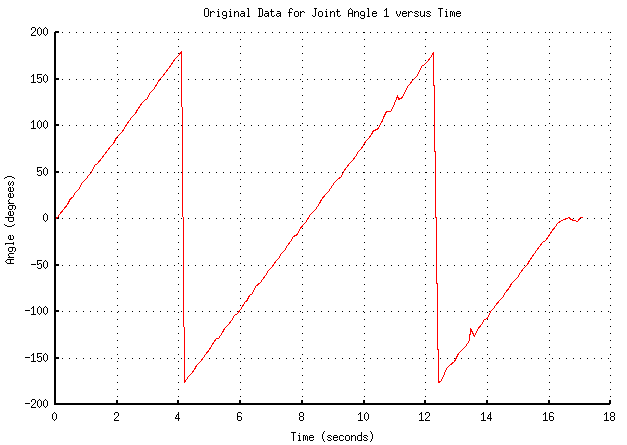
\includegraphics[width=4in]{images/dataacq1_plot1.png}
\caption{\label{fig:dataacq1_fig1} The original data recorded by \texttt{dataAcquisition.ch}.}
\end{figure}

Figure \ref{fig:dataacq1_fig1} appears to show
a zig-zag pattern for the angle of the joint. This is because the raw angle data obtained
from a Mobot is only in the range -180 degrees to 180 degrees. When a joint rotates
past 180 degrees, the angle reading switches over -180 degrees. In order to get rid of the
zig-zagging of the data, the data must be ``unwrapped''. This is done with the \texttt{unwrapdeg()}
function, as done in the following line of code:
\begin{verbatim}
unwrapdeg(angles1_unwrapped, angles1);
\end{verbatim}
The function places the unwrapped version of the \texttt{angles1} array into our array
\texttt{angles1\_unwrapped}. Next, we plot the unwrapped data in a similar method 
to plotting our wrapped data:
\begin{verbatim}
plot2.title("Unwrapped Data for Joint Angle 1 versus Time");
plot2.label(PLOT_AXIS_X, "Time (seconds)");
plot2.label(PLOT_AXIS_Y, "Angle (degrees)");
plot2.data2DCurve(time, angles1_unwrapped, numDataPoints);
plot2.grid(PLOT_ON);
plot2.plotting();
\end{verbatim}

\begin{figure}[H]
\centering
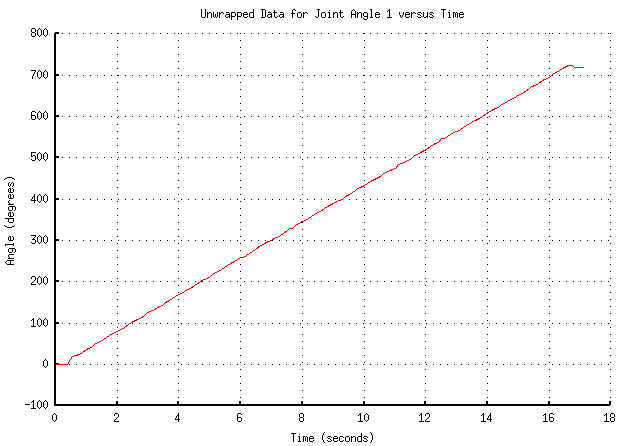
\includegraphics[width=4in]{images/dataacq1_plot2.png}
\caption{\label{fig:dataacq1_fig2} The unwrapped data recorded by \texttt{dataAcquisition.ch}.}
\end{figure}

Figure \ref{fig:dataacq1_fig2} displays the unwrapped data. It shows the motion as 
one fluid motion starting at 0 degrees and ending at 720 degrees. 

Finally, we want to generate a plot where the beginning of the motion correctly starts
at time 0. Looking at Figure \ref{fig:dataacq1_fig2}, you will notice that there is about
a fraction of a second delay before the joints actually start moving. For our final plot, we want
to display a plot of the same data, but shifted to the left so that the motion starts at
time zero. This will make it easier to verify the speed of the joint and the time it takes
to get to 720 degrees. 

To do this, we use the \texttt{shiftTime()} function. The \texttt{shiftTime()} function
is used to shift graphs of data to the left by detecting the first moment a joint begins
moving. The following code shifts the data to the left so that it appears that the motion begins
right at time 0.
\begin{verbatim}
shiftTime(tolerance, numDataPoints, time, angles1Unwrapped);
\end{verbatim}

Finally, we plot the shifted data.

\begin{verbatim}
plot3.title("Unwrapped and shifted Data for Joint Angle 1 versus Time");
plot3.label(PLOT_AXIS_X, "Time (seconds)");
plot3.label(PLOT_AXIS_Y, "Angle (degrees)");
plot3.data2DCurve(time, angles1_unwrapped, numDataPoints);
plot3.grid(PLOT_ON);
plot3.plotting();
\end{verbatim}

\begin{figure}[H]
\centering
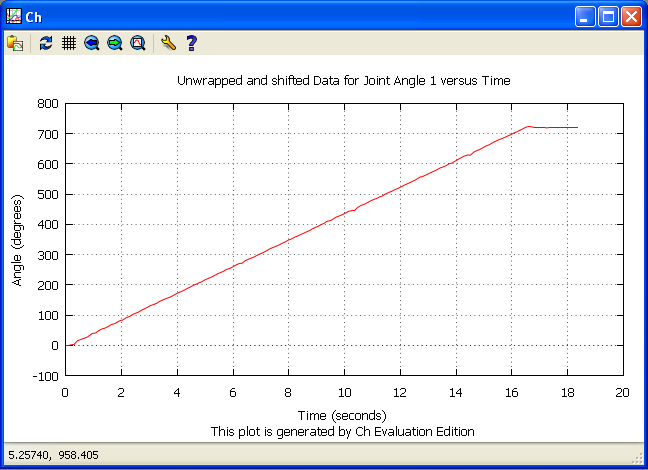
\includegraphics[width=4in]{images/dataacq1_plot3.png}
\caption{\label{fig:dataacq1_fig3} The unwrapped and shifted data recorded by \texttt{dataAcquisition.ch}.}
\end{figure}

Figure \ref{fig:dataacq1_fig3}  displays our unwrapped data that has been time shifted. It can be seen
that the beginning of the motion now happens at time 0, and it may be verified that the
line generated is very close to the expected function, $\theta = 45 t$.

In many applications, the user may only be interested in the unwrapped, time shifted data. 
In such a case, a simplified version of the program may be used. The program 
\texttt{dataAcquisition1.ch} below removes the intermediate plots and can be modified
to solve other data acquisition problems.

\subsubsection{\texttt{dataAcquisition1.ch} Source Code}
\verbatiminput{../demos/chdemos/dataAcquisition1.ch}

\subsection{Example 2}
It is also possible to record the joint angles for all four joints simultaneously
with the \texttt{recordAngles()} function. The function is conceptually similar
to \texttt{recordAngle()}, except that it obtains 4 joint angles for each timestamp.

\subsubsection{Problem Statement}
Record and plot the motion of all 4 joints of the Mobot as it performs the
following two motions:
\begin{enumerate}
\item Turn right by rotating joints 360 degrees.
\item Inchworm to the left twice.
\end{enumerate}

\subsubsection{\texttt{dataAcquisition2.ch} Source Code}
\verbatiminput{../demos/chdemos/dataAcquisition2.ch}

\subsubsection{\texttt{dataAcquisition2.ch} Explained}
Similar to the previous data acquisition demo, we begin by including
header files, declaring our mobot variable, and connecting to the mobot:
\begin{verbatim}
#include <mobot.h>
#include <chplot.h>
#include <numeric.h>
CMobot mobot;

/* Connect to the mobot */
mobot.connect();
\end{verbatim}

We also set our data acquisition interval, movement time, and calculate
the number of data points:
\begin{verbatim}
double timeInterval = 0.1; /* Seconds */

/* Record for 20 seconds */
double movementTime = 20;
int numDataPoints = movementTime / timeInterval; /* Unitless */
\end{verbatim}
For this motion, the value of 20 seconds was decided through trial-and-error.
For complex motions such as inchworming, it is difficult to accurately estimate the 
amount of time the motion will take to complete. Through experimentation and experience,
it was determined that 20 seconds allowed for a sufficient amount of time to record the 
turning motion and the inchworming motion. 

Next, we declare our computational arrays for storing data and plotting, similar to 
the previous demo. One main difference is we declare a separate computational array
to store data for each joint angle.
\begin{verbatim}
/* Initialize the arrays to be used to store data */
array double time[numDataPoints];
array double angles1[numDataPoints];
array double angles2[numDataPoints];
array double angles3[numDataPoints];
array double angles4[numDataPoints];

/* Declare plotting variables */
CPlot plot1, plot2;
array double angles1_unwrapped[numDataPoints];
array double angles2_unwrapped[numDataPoints];
array double angles3_unwrapped[numDataPoints];
array double angles4_unwrapped[numDataPoints];
double tolerance = 1.0; /* 1 degree for time shifting */
\end{verbatim}

Before we begin the motion, we set all the joint speeds to 45 degrees/second
and move the mobot into its zero postition.
\begin{verbatim}
/* Set all joint speeds to 45 degrees/second */
mobot.setJointSpeeds(45, 45, 45, 45);

/* Start the motion. First, move mobot to zero position */
mobot.moveToZero();
\end{verbatim}

Next, we begin recording the data.
\begin{verbatim}
mobot.recordAngles(time, angles1, angles2, angles3, angles4, numDataPoints, timeInterval);
\end{verbatim}

Similar to \texttt{recordAngle()}, the recording process occurs in the background as
the main program continues. We next execute our desired motions, which are to turn the
mobot to the right by rotating each wheel 360 degrees, and then inchworming to
the left twice:
\begin{verbatim}
mobot.motionTurnRight(360);
mobot.motionInchwormLeft(2);
\end{verbatim}

Finally, we wait for the recording to finish.
\begin{verbatim}
mobot.recordWait();
\end{verbatim}

Now that all of the data has been acquired, we unwrap, shift, and plot the data.
\begin{verbatim}
unwrapdeg(angles1_unwrapped, angles1);
unwrapdeg(angles2_unwrapped, angles2);
unwrapdeg(angles3_unwrapped, angles3);
unwrapdeg(angles4_unwrapped, angles4);
/* Shift the time so the movement starts at time 0 */
shiftTime(tolerance, numDataPoints, time, 
          angles1_unwrapped, 
          angles2_unwrapped, 
          angles3_unwrapped, 
          angles4_unwrapped);
plot2.title("Unwrapped Data for Joint Angles versus Time");
plot2.label(PLOT_AXIS_X, "Time (seconds)");
plot2.label(PLOT_AXIS_Y, "Angle (degrees)");
plot2.data2DCurve(time, angles1_unwrapped, numDataPoints);
plot2.data2DCurve(time, angles2_unwrapped, numDataPoints);
plot2.data2DCurve(time, angles3_unwrapped, numDataPoints);
plot2.data2DCurve(time, angles4_unwrapped, numDataPoints);
plot2.legend("Joint 1", 0);
plot2.legend("Joint 2", 1);
plot2.legend("Joint 3", 2);
plot2.legend("Joint 4", 3);
plot2.grid(PLOT_ON);
plot2.plotting();
\end{verbatim}
Note that the previous call to \texttt{shiftTime()} appears different than the previous
example. The \texttt{shiftTime()} function is able to accept any number of data
arrays per time array to shift. The function tests the tolerance angle on all of the
input data arrays, seeking the first occurance of a movement greater than the tolerance
for all of the data arrays. This makes the plotted motion begin right at time 0 on
the plot.

\begin{figure}[H]
\centering
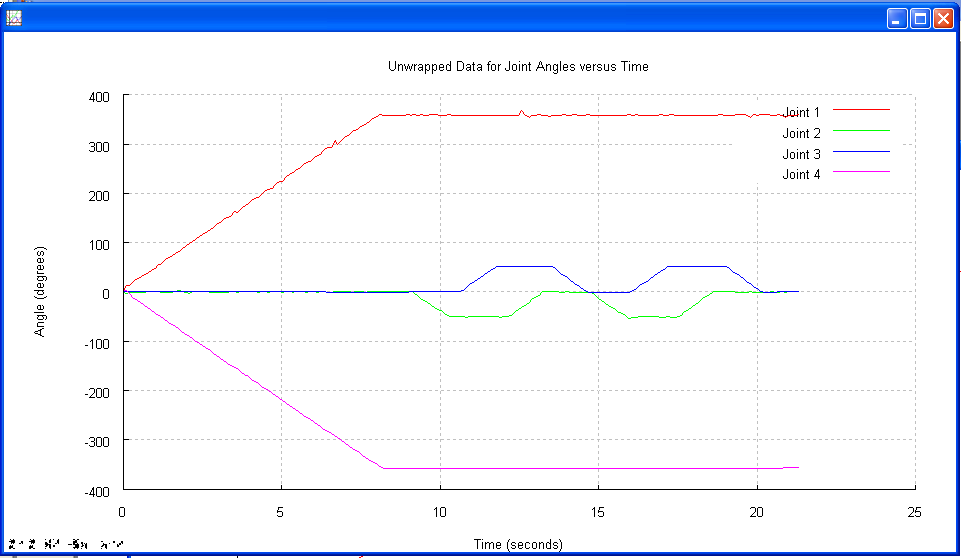
\includegraphics[width=4in]{images/dataacq2_plot1.png}
\caption{\label{fig:dataacq2_fig1} The unwrapped and shifted data recorded by \texttt{dataAcquisition2.ch}.}
\end{figure}

Figure \ref{fig:dataacq2_fig1} shows the captured data from the Mobot. During the first
part of the motions, joints 1 and 4 move in opposite directions to rotate the mobot to
the right. After rotating 360 degrees, joints 2 and 3 move to inchworm the mobot to the
left twice.

\subsection{Example 3}
\subsubsection{Problem Statement}
A mobot is equipped with 3.5 inch diameter wheels. Write a piece of code which rolls the
mobot forward at constant speed of 2.5 inches per second for a distance of 12 inches. 
Verify that the data is linear and follows the relation $d = 2.5t$

\subsubsection{\texttt{dataAcquisition3.ch} Source Code}
\verbatiminput{../demos/chdemos/dataAcquisition3.ch}

\subsubsection{\texttt{dataAcquisition3.ch} Explained}
The first lines include header files and set up the mobot similar to the previous
demos:
\begin{verbatim}
#include <mobot.h>
#include <chplot.h>
#include <numeric.h>
CMobot mobot;

/* Connect to the mobot */
mobot.connect();
\end{verbatim}

Next, we initialize some variables. First, we make a variable to store the speed
we want to move the mobot.
\begin{verbatim}
double speed = 2.5; /* inches / second */
\end{verbatim}

Next, a variable for the distance.
\begin{verbatim}
double distance = 12; /* inches */
\end{verbatim}

And a variable for the wheel radius...
\begin{verbatim}
double radius = 3.5/2.0; /* inches */
\end{verbatim}

Now we wish to calculate the angle that the wheels need to turn in order to
travel a distance of 12 inches. To do this, we use a function called
\texttt{distance2angle()}. The \texttt{distance2angle()} function 
takes a wheel radius and the distance as arguments and returns the angle
the wheel must turn to travel that distance. 
\begin{verbatim}
double angle = distance2angle(radius, distance); /* degrees */
\end{verbatim}

Internally, the angle in degrees is calculated by the formula
\begin{equation*}
\theta  = \left(\frac{d}{r} \right) * 180 / \pi
\end{equation*}
where $\theta$ is the angle in degrees, $d$ is the distance travelled, 
and $r$ is the radius of the wheel.

For the next step, we must calculate our estimated movement time, similar to the
\texttt{dataAcquisition.ch} demo presented earlier. 
\begin{verbatim}
double movementTime = distance / speed; /* Seconds */
\end{verbatim}

Is in previous demos, we include an extra second in our movement time. We
also calculate the number of data points based on the total movement time
and the time interval.
\begin{verbatim}
movementTime = movementTime + 1; 
double timeInterval = 0.1; /* seconds */
int numDataPoints = movementTime / timeInterval; /* Unitless */
\end{verbatim}

Now, we allocate our computational arrays for storing data. We have arrays 
for the time, angles, and also distances.
\begin{verbatim}
array double time[numDataPoints];
array double angles1[numDataPoints];
array double distances[numDataPoints];

/* Declare plotting variables */
CPlot plot;
array double angles1Unwrapped[numDataPoints];
double tolerance = 1.0; /* Degrees */
\end{verbatim}

Before beginning the motion, we move the mobot to zero position and set the 
wheel speeds.
\begin{verbatim}
/* Start the motion. First, move mobot to zero position */
mobot.moveToZero();
/* Set mobot wheel speed */
mobot.setTwoWheelRobotSpeed(speed, radius);
\end{verbatim}

Start recording the angle of the first joint.
\begin{verbatim}
mobot.recordAngle(MOBOT_JOINT1, time, angles1, numDataPoints, timeInterval);
\end{verbatim}

Move the mobot forward by the angle calculated earlier with \texttt{distance2angle()}.
\begin{verbatim}
mobot.motionRollForward(angle);
\end{verbatim}

Wait for the recording to finish.
\begin{verbatim}
mobot.recordWait();
\end{verbatim}

Finally, we want to unwrap and shift the data and convert the angle readings to a distance.
The unwrap and shifting process is identical to Example 1 of this section. 
We convert the angles back to a distance using the \texttt{angle2distance()} function,
which takes the radius of a wheel and the angle moved in degrees as arguments and
return the distance traveled. The arguments can be single variables or computational
arrays. If the angle argument is a computational array, the value returned is also
a computational array. The \texttt{angle2distance()} function converts the angle
to a distance using the following formula.
\begin{equation*}
d = \left(\theta \frac{\pi}{180}\right) r
\end{equation*}
where $d$ is the distance travelled, $\theta$ is the angle rotated in degrees, and $r$ is the
radius of the wheel. The units of distance for $d$ will be the same units as those
chosen for $r$. For instance, if $r$ is expressed in inches, the result 

\begin{verbatim}
/* Unwrap the data */
unwrapdeg(angles1_unwrapped, angles1);
/* Shift the data */
shiftTime(tolerance, numDataPoints, time, angles1Unwrapped);
/* Convert angles to displacement */
distances = angle2distance(radius, angles1Unwrapped);
\end{verbatim}

Finally, we create a plot of the data.
\begin{verbatim}
plot.title("Displacement versus Time");
plot.label(PLOT_AXIS_X, "Time (seconds)");
plot.label(PLOT_AXIS_Y, "Displacement (inches)");
plot.data2DCurve(time, distances, numDataPoints);
plot.grid(PLOT_ON);
plot.plotting();
\end{verbatim}

\begin{figure}[H]
\centering
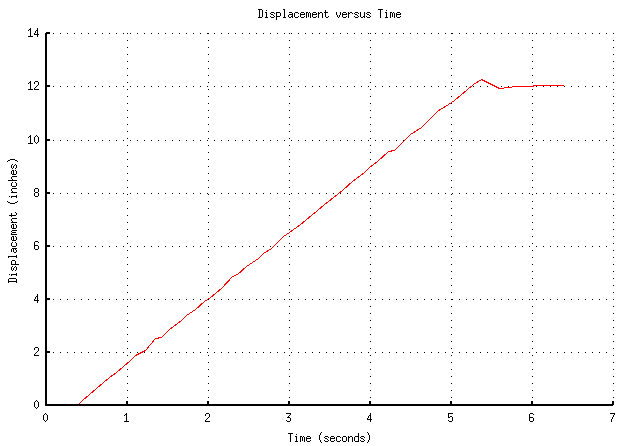
\includegraphics[width=4in]{images/dataacq3_plot1.png}
\caption{\label{fig:dataacq3_fig1} The unwrapped data recorded by \texttt{dataAcquisition2.ch}.}
\end{figure}

Figure \ref{fig:dataacq3_fig1} displays the distance data acquired during the motion. It can
be seen that the mobot traveled to a distance of 12 inches, and then stopped. The
expected relation between time and distance is the linear function 
\begin{equation*}
d = 2.5t
\end{equation*}
which may be verified on the graph. Furthermore, the time that it should take to reach 
12 inches is 
\begin{equation}
t = d / 2.5 = 12 / 2.5 = 4.8 ~\text{seconds}
\end{equation}
which may also be verified from the graph.

\section{Using the On-Board Buttons}
\subsection{Running the On-Board Joint Test program}
The Mobot comes with a demo test program hard-coded into the on-board
computer. The test program is designed to test the Mobot's joints range of 
motion and make sure everything is working properly. The test program will
move the mobot continuously until the Mobot is shut off.

To run the test program, simply hold the ``A'' button for 3 seconds. After
3 seconds have passed, the blue LED should blink 3 times quickly, and the
demo motion will begin.

\subsection{Recalibrating the Mobot's Zero Position}
A user may recalibrate the Mobot's zero positions if necessary. To recalibrate
the Mobot, perform the following steps:
\begin{itemize}
\item Position the Mobot into its zero position. If the Mobot is currently
actuating any of its joints, or if any joints feel ``stiff'', you may power the
Mobot off and on again.
\item While the Mobot is powered on, press both the ``A'' and ``B'' buttons
simultaneously. The blue LED should flash quickly 3 times. The Mobot has now
been recalibrated.
\end{itemize}

\subsection{\label{sec:zeroposition}Testing the Mobot's Zero Position}
Button ``B'' may be used to toggle the mobot between holding its zero position 
or relaxing all of its joints. Press and hold the ``B'' button until the blue
LED flashes. It should take no longer than 1 second. If the Mobot is currently relaxed,
the Mobot will move to zero position and hold its position. If the ``B'' button is pressed again, the 
Mobot will relax its motors, allowing the user to reposition the Mobot.

This function is typically used to check the Mobot's zero position to make sure
it is properly calibrated. The button may also be used to relax a Mobot that
is currently holding any of its joints at a position.

\newpage
\appendix
\section{CMobot Class}
\subsection{\label{sec:datatypes}Data Types}
The data types defined in the header file \texttt{mobot.h} are described in
this appendix.
These data types are used by the Mobot library to represent 
certain values, such as joint id's and motor directions.

\begin{tabular}{p{3.5cm}p{10cm}} \hline 
Data Type& Description \\
\hline 
\texttt{mobotJointId\_t} & An enumerated value that indicates a Mobot joint. \\
\texttt{mobotJointState\_t} & The current state of a Mobot joint. \\
\hline
\end{tabular}

\subsection{\label{sec:mobotJointId_t}\texttt{mobotJointId\_t}}
This datatype is an enumerated type used to identify a joint on the Mobot. Valid
values for this type are:
\begin{verbatim}
typedef enum mobot_joints_e {
  MOBOT_JOINT1 = 1,
  MOBOT_JOINT2 = 2,
  MOBOT_JOINT3 = 3,
  MOBOT_JOINT4 = 4
} mobotJointId_t;
\end{verbatim}
\index{mobot\_joints\_t}

\index{MOBOT\_JOINT1}
\index{MOBOT\_JOINT2}
\index{MOBOT\_JOINT3}
\index{MOBOT\_JOINT4}
\begin{tabular}{p{3cm}p{10cm}} \hline 
Value & Description \\
\hline 
\texttt{MOBOT\_JOINT1} & Joint number 1 on the Mobot, which is a faceplate joint. \\
\texttt{MOBOT\_JOINT2} & Joint number 2 on the Mobot, which is a body joint. \\
\texttt{MOBOT\_JOINT3} & Joint number 3 on the Mobot, which is a body joint. \\
\texttt{MOBOT\_JOINT4} & Joint number 4 on the Mobot, which is a faceplate joint. \\
\hline
\end{tabular}

\subsection{\label{sec:mobotJointState_t}\texttt{mobotJointState\_t}}
This datatype is an enumerated type used to designate the current 
movement state of a joint. The values may be retrieved from the 
mobot with the \texttt{getJointState()} function and may be set 
with the \texttt{moveContinuous()} family of functions. Valid values are:

\begin{verbatim}
typedef enum mobot_joint_state_e {
  MOBOT_NEUTRAL   = 0,
  MOBOT_FORWARD   = 1,
  MOBOT_BACKWARD  = 2,
  MOBOT_HOLD      = 3
} mobotJointState_t;
\end{verbatim}

\begin{tabular}{p{3.3cm}p{11.5cm}} \hline 
Value & Description \\
\hline
\texttt{MOBOT\_NEUTRAL}& This value indicates that the joint is not moving and is not actuated. The joint is freely backdrivable. \\
\texttt{MOBOT\_FORWARD}& This value indicates that the joint is currently moving forward. \\
\texttt{MOBOT\_BACKWARD}& This value indicates that the joint is currently moving backward. \\
\texttt{MOBOT\_HOLD}& This value indicates that the joint is currently not moving and is holding its current position. The joint is not currently backdrivable. \\
\hline
\end{tabular}

\subsection{\label{sec:cmobot_api}CMobot API Functions}
%\lhead{libimobotcomms API Documentation}
\noindent
The header file {\bf mobot.h} defines all the data types, macros 
and function prototypes for the mobot API library. The header file
declares a class called \texttt{CMobot} which contains member functions which
may be used to control the mobot.

\begin{table}[!h]
%\capstart
\begin{center}
\caption{CMobot Member Functions.}
\begin{tabular}{p{48 mm}p{110 mm}}
%\begin{tabular}{ll}
\hline
Function & Description \\
\hline
%\texttt{pose()} \dotfill & Pose multiple joints of the mobot. \\
\texttt{CMobot()} & The CMobot constructor function. This function
is called automatically and should not be called explicitly. \\
\texttt{\textasciitilde CMobot()} & The CMobot destructor function. This function
is called automatically and should not be called explicitly. \\
& \\
\texttt{blinkLED()} & Blink the LED on a Mobot module. \\
\texttt{connect()} & Connect to a remote mobot module. This function 
connects to the first mobot listed in the Barobo configuration file. To
edit the configuration file, use the mobot control graphical user interface,
and select the menu item ``Mobot $\rightarrow$ Configure Mobot Bluetooth''. \\
\texttt{connectWithBluetoothAddress()} & Connect to a mobot module by specifying its Bluetooth address. \\
\texttt{connectWithIPAddress()} & Connect to a mobot module by specifying a remote computer's IP address. \\
\texttt{disconnect()} & Disconnect from a mobot module. \\
\texttt{disableButtonCallback()} & Reverts a Mobot's buttons to their factory-default functions. \\
\texttt{driveTo()} & Move all four joints of the mobot to specified absolute angles. \\
\texttt{driveToNB()} & Move all four joints of the mobot to specified absolute angles. \\
\texttt{enableButtonCallback()} & Enables a user-driven callback for handling button-press events on a module. \\
\texttt{getJointAngle()} & Get a joint's angle. \\
\texttt{getJointAngles()} & Get joint angles for all joints. \\
%\texttt{getJointDirection()} & Gets a motor's currently assigned direction. \\
\texttt{getJointMaxSpeed()} & Get a joint's maximum speed in radians per second. \\
\texttt{getJointSafetyAngle()} & Get the mobot's safety angle limit. \\
\texttt{getJointSafetyAngleTimeout()} & Get the mobot's safety angle limit timeout. \\
\texttt{getJointSpeed()} & Get a motor's current speed setting in radians per second. \\
\texttt{getJointSpeeds()} & Get all motor's current speed settings in radians per second. \\
\texttt{getJointSpeedRatio()} & Get a motor's speed as a ratio of the motor's maximum speed. \\
\texttt{getJointSpeedRatios()} & Get all motor speeds as ratios of the motor's maximum speed. \\
\texttt{getJointState()} & Get a motor's current status. \\
\texttt{isConnected()} & This function is used to check the connection to a mobot. \\
\texttt{isMoving()} & This function is used to check if any joints are currently in motion. \\
\texttt{move()} & Move all four joints of the mobot by specified angles. \\
\texttt{moveNB()} & Identical to \texttt{move()} but non-blocking. \\
\texttt{moveContinuousNB()} & Move joints continuously. Joints will move untill stopped.\\
\texttt{moveContinuousTime()} & Move joints continuously for a certain amount of time.\\
\texttt{moveJoint()} & Move a joint. \\
\texttt{moveJointContinuousNB()} & Move a joint continuously. \\
\texttt{moveJointContinuousTime()} & Move a joint continuously for a certain amount of time. \\
\texttt{moveJointNB()} & Move a joint. \\
\texttt{moveJointTo()} & Set the desired motor position for a joint. \\
\texttt{moveJointToNB()} & Identical to \texttt{moveJointTo()} but non-blocking. \\
\texttt{moveJointWait()} & Wait until the specified motor has stopped moving. \\
\texttt{moveTo()} & Move all four joints of the mobot to specified absolute angles. \\
\texttt{moveToNB()} & Identical to \texttt{moveTo()} but non-blocking. \\
\texttt{moveToZero()} & Instruct all motors to go to their zero positions. \\
\texttt{moveToZeroNB()} & Identical to \texttt{moveToZero()} but non-blocking. \\
\texttt{moveWait()} & Wait until all motors have stopped moving. \\
%\texttt{setJointDirection()} & Set the motor direction of a motor. Set
%to "0" for automatic direction, "1" for forward, and "2" for reverse. \\
\texttt{recordAngle()} & Begin recording the angle of a joint. \\
\texttt{recordAngleBegin()} & Begin recording the angle of a joint. \\
\texttt{recordAngleEnd()} & End recording the angle of a joint. \\
\texttt{recordAngles()} & Begin recording the angle of all joints. \\
\texttt{recordAnglesBegin()} & Begin recording the angle of all joints. \\
\texttt{recordAnglesEnd()} & End recording the angle of all joints. \\
\texttt{recordWait()} & Wait for recording operations to finish. \\
\hline
\end{tabular}
\end{center}
\label{mobilec_api_cbinary}
\end{table}

\addtocounter{table}{-1}

\begin{table}[!h]
%\capstart
\begin{center}
\caption{CMobot Member Functions (Continued)}
\begin{tabular}{p{48 mm}p{110 mm}}
%\begin{tabular}{ll}
\hline
Function & Description \\
\hline
\texttt{resetToZero()} & Instruct all motors to go to their zero positions. \\
\texttt{setJointMovementStateNB()} & Set the movement state of a joint. \\
\texttt{setJointMovementStateTime()} & Set the movement state of a joint for a period of time.\\
\texttt{setJointSafetyAngle()} & Set the mobot's safety angle limit. The default value is 10 degrees.\\
\texttt{setJointSafetyAngleTimeout()} & Set the mobot's safety angle limit timeout. The default value is 0.5 seconds.\\
\texttt{setJointSpeed()} & Set a motor's speed setting in radians per second. \\
\texttt{setJointSpeeds()} & Set all motor speeds in radians per second. \\
\texttt{setJointSpeedRatio()} & Set a joints speed setting to a fraction of its maximum speed, a value between 0 and 1. \\
\texttt{setJointSpeedRatios()} & Set all joint speed settings to a fraction of its
maximum speed, expressed as a value from 0 to 1. \\
\texttt{setMovementStateNB()} & Change the movement states of the joints. Movement states include moving forward, backward, neutral, or holding their current position.\\
\texttt{setMovementStateTime()} & Change the movement states of the joints for a certain amount of time.\\
\texttt{stopAllJoints()} & Stop all currently executing motions of the mobot. \\
\texttt{stopOneJoint()} & Stop a joint on the mobot. \\
\texttt{stopTwoJoints()} & Stop two joints on the mobot. \\
\texttt{stopThreeJoints()} & Stop three joints on the mobot. \\
\hline
\end{tabular}
\end{center}
\label{mobilec_api_cbinary}
\end{table}

\begin{table}[!h]
%\capstart
\begin{center}
\caption{CMobot Member Functions for Compound Motions.}
\begin{tabular}{p{38 mm}p{107 mm}}
Compound Motions & These are convenience functions of commonly used compound motions. \\
\hline
\texttt{motionArch()} \dotfill & Arch the mobot for better ground clearance. \\
\texttt{motionArchNB()} \dotfill & Identical to \texttt{motionArch} but non-blocking. \\
\texttt{motionInchwormLeft()} \dotfill & Inchworm motion towards the left. \\
\texttt{motionInchwormLeftNB()} \dotfill & Identical to \texttt{motionInchwormLeft} but non-blocking. \\
\texttt{motionInchwormRight()} \dotfill & Inchworm motion towards the right. \\
\texttt{motionInchwormRightNB()} \dotfill & Identical to \texttt{motionInchwormRight} but non-blocking. \\
\texttt{motionRollBackward()} \dotfill & Roll on the faceplates toward the backward direction. \\
\texttt{motionRollBackwardNB()} \dotfill & Identical to \texttt{motionRollBackward()} but non-blocking. \\
\texttt{motionRollForward()} \dotfill & Roll on the faceplates forwards. \\
\texttt{motionRollForwardNB()} \dotfill & Identical to \texttt{motionRollForward()} but non-blocking. \\
\texttt{motionSkinny()} \dotfill & Move the mobot into a skinny profile. \\
\texttt{motionSkinnyNB()} \dotfill & Identical to \texttt{motionSkinny()} but non-blocking. \\
\texttt{motionStand()} \dotfill & Stand the mobot up on its end. \\
\texttt{motionStandNB()} \dotfill & Identical to \texttt{motionStand()} but non-blocking. \\
\texttt{motionTumbleLeft()} \dotfill & Perform the tumbling motion. \\
\texttt{motionTumbleLeftNB()} \dotfill & Identical to \texttt{motionTumbleLeft()} but non-blocking. \\
\texttt{motionTumbleRight()} \dotfill & Perform the tumbling motion in the opposite direction of ``motionTumbleLeft''. \\
\texttt{motionTumbleRightNB()} \dotfill & Identical to \texttt{motionTumbleRight()} but non-blocking. \\
\texttt{motionTurnLeft()} \dotfill & Rotate the mobot counterclockwise. \\
\texttt{motionTurnLeftNB()} \dotfill & Identical to \texttt{motionTurnLeft()} but non-blocking. \\
\texttt{motionTurnRight()} \dotfill & Rotate the mobot clockwise. \\
\texttt{motionTurnRightNB()} \dotfill & Identical to \texttt{motionTurnRight()} but non-blocking. \\
\texttt{motionWait()} \dotfill & Wait for a motion to finish. \\
\hline
\end{tabular}
\end{center}
\label{mobilec_api_compound}
\end{table}

\clearpage
\newpage
\noindent
\vspace{5pt}
\rule{4.5in}{0.015in}\\
\noindent
{\LARGE \texttt{CMobot::blinkLED()}\index{CMobot::blinkLED()}}\\
%\phantomsection
\addcontentsline{toc}{section}{blinkLED()}

\noindent
{\bf Synopsis}
\vspace{-8pt}
\begin{verbatim}
#include <mobot.h>
int CMobot::blinkLED(double delay, int numBlinks);
\end{verbatim}

\noindent
{\bf Purpose}\\
Blink the on-board LED on a Mobot module.\\

\noindent
{\bf Return Value}\\
The function returns 0 on success and non-zero otherwise.\\

\noindent
{\bf Parameters}\\
\vspace{-0.1in}
\begin{description}
\item               
\begin{tabular}{p{15 mm}p{125 mm}}
\texttt{delay} & The amount of time between blinks. \\
\texttt{numBlinks} & The number of times to blink the LED. \\
\end{tabular}
\end{description}
\noindent
{\bf Description}\\
This function is used to blink or flash the LED on a Mobot module. The first
argument, \texttt{delay}, is used to control the speed of the blinking
LED, and the second argument, \texttt{numBlinks}, controls the number of times
to blink. For instance, the line
\begin{verbatim}
mobot.blinkLED(0.1, 10);
\end{verbatim}
would cause a mobot to blink 10 times fast, and the line
\begin{verbatim}
mobot.blinkLED(1, 2);
\end{verbatim}
would cause the mobot to do two slow blinks.

\noindent
{\bf Example}\\
\noindent

\noindent
{\bf See Also}\\

%\CPlot::\DataThreeD(), \CPlot::\DataFile(), \CPlot::\Plotting(), \plotxy().\\

\noindent
\vspace{5pt}
\rule{4.5in}{0.015in}\\
\noindent
{\LARGE \texttt{CMobot::connect()}\index{connect()}}\\
%\phantomsection
\addcontentsline{toc}{section}{connect()}

\noindent
{\bf Synopsis}\\
\begin{verbatim}
#include <mobot.h>
int CMobot::connect();
\end{verbatim}

\noindent
{\bf Purpose}\\
Connect to a remote iMobot via Bluetooth.\\

\noindent
{\bf Return Value}\\
The function returns 0 on success and non-zero otherwise.\\

\noindent
{\bf Parameters}\\
None.\\

\noindent
{\bf Description}\\
This function is used to connect to an iMobot. The iMobot must first be paired
with the computer. This function currently only works in Microsoft Windows
operating systems. For other operating systems, please use the
\texttt{connectAddress()} function.

\noindent
{\bf Example}\\
Please see the example in Section \ref{sec:democode} on page \pageref{sec:democode}.\\
\noindent

\noindent
{\bf See Also}\\
\texttt{connectAddress()}

%\CPlot::\DataThreeD(), \CPlot::\DataFile(), \CPlot::\Plotting(), \plotxy().\\

\noindent
\vspace{5pt}
\rule{4.5in}{0.015in} \\
\noindent
{\LARGE \texttt{CMobot::connectWithBluetoothAddress()}\index{CMobot::connectWithBluetoothAddress()}}\\
%\phantomsection
\addcontentsline{toc}{section}{connectWithBluetoothAddress()}

\noindent
{\bf Synopsis}
\vspace{-8pt}
\begin{verbatim}
#include <mobot.h>
int CMobot::connectWithBluetoothAddress(char address[], int channel = 1);
\end{verbatim}

\noindent
{\bf Purpose}\\
Connect to a remote mobot via Bluetooth by specifying the specific Bluetooth
address of the device.\\

\noindent
{\bf Return Value}\\
The function returns 0 on success and non-zero otherwise.\\

\noindent
{\bf Parameters}
\vspace{-0.1in}
\begin{description}
\item               
\begin{tabular}{p{10 mm}p{145 mm}}
\texttt{address} & The Bluetooth address of the mobot. \\
\texttt{channel} & (optional) The Bluetooth channel that the listening program is
listening on. The default channel is channel 1. \\
\end{tabular}
\end{description}

\noindent
{\bf Description}\\
This function is used to connect to a mobot. 

\noindent
{\bf Example}\\
\begin{verbatim}
mobot.connectWithBluetoothAddress("00:06:66:45:DA:02", 1);
mobot.connectWithBluetoothAddress("00:06:66:45:DA:F3");
\end{verbatim}
\noindent

\noindent
{\bf See Also}\\
\texttt{connect(), disconnect()}

%\CPlot::\DataThreeD(), \CPlot::\DataFile(), \CPlot::\Plotting(), \plotxy().\\

\noindent
\vspace{5pt}
\rule{4.5in}{0.015in} \\
\noindent
{\LARGE \texttt{CMobot::connectWithIPAddress()}\index{CMobot::connectWithIPAddress()}}\\
%\phantomsection
\addcontentsline{toc}{section}{connectWithIPAddress()}

\noindent
{\bf Synopsis}
\vspace{-8pt}
\begin{verbatim}
#include <mobot.h>
int CMobot::connectWithIPAddress(char address[], char port[] = "5768");
\end{verbatim}

\noindent
{\bf Purpose}\\
Connect to a remote mobot connected to a remote computer over the internet.\\

\noindent
{\bf Return Value}\\
The function returns 0 on success and non-zero otherwise.\\

\noindent
{\bf Parameters}
\vspace{-0.1in}
\begin{description}
\item               
\begin{tabular}{p{10 mm}p{145 mm}}
\texttt{address} & The IP address of the remote computer. \\
\texttt{port} & (optional) The port to connect to. \\
\end{tabular}
\end{description}

\noindent
{\bf Description}\\
This function is used to connect to a mobot. 

\noindent
{\bf Example}\\
mobot.connectWithIPAddress("192.168.0.132", "8734");
mobot.connectWithIPAddress("mobots.example.com", "5768");
mobot.connectWithIPAddress("192.168.100.221");
\noindent

\noindent
{\bf See Also}\\
\texttt{connect(), disconnect()}

%\CPlot::\DataThreeD(), \CPlot::\DataFile(), \CPlot::\Plotting(), \plotxy().\\

\noindent
\vspace{5pt}
\rule{4.5in}{0.015in}\\
\noindent
{\LARGE \texttt{CMobot::disconnect()}\index{CMobot::disconnect()}}\\
%\phantomsection
\addcontentsline{toc}{section}{disconnect()}

\noindent
{\bf Synopsis}\\
\begin{verbatim}
#include <mobot.h>
int CMobot::disconnect();
\end{verbatim}

\noindent
{\bf Purpose}\\
Disconnect from a remote robot.\\

\noindent
{\bf Return Value}\\
The function returns 0 on success and non-zero otherwise.\\

\noindent
{\bf Parameters}\\
None.\\

\noindent
{\bf Description}\\
This function is used from disconnect to a robot. A call to this function is
not necessary before the termination of a program. It is only necessary if
another connection will be established within the same program at a later time.
\\

\noindent
{\bf Example}\\
\noindent

\noindent
{\bf See Also}\\
\texttt{connect(), connectWithAddress()}

%\CPlot::\DataThreeD(), \CPlot::\DataFile(), \CPlot::\Plotting(), \plotxy().\\

\noindent
\vspace{5pt}
\rule{4.5in}{0.015in}\\
\noindent
{\LARGE \texttt{CMobot::driveJointTo()}\index{CMobot::driveJointTo()}}\\
{\LARGE \texttt{CMobot::driveJointToNB()}\index{CMobot::driveJointToNB()}}\\
%\phantomsection
\addcontentsline{toc}{section}{driveJointTo()}
\addcontentsline{toc}{section}{driveJointToNB()}

\noindent
{\bf Synopsis}
\vspace{-8pt}
\begin{verbatim}
#include <mobot.h>
int CMobot::driveJointTo(moboJointId_t id, double angle);
int CMobot::driveJointToNB(moboJointId_t id, double angle);
\end{verbatim}

\noindent
{\bf Purpose}\\
Move all of the joints of a mobot to the specified positions.\\

\noindent
{\bf Return Value}\\
The function returns 0 on success and non-zero otherwise.\\

\noindent
{\bf Parameters}\\
\vspace{-0.1in}
\begin{description}
\item               
\begin{tabular}{p{15 mm}p{105 mm}}
\texttt{id} & The id of the joint to move. \\
\texttt{angle} & The absolute position to move the joint, expressed in degrees. \\
\end{tabular}
\end{description}
\noindent

{\bf Description}\\
\vspace{-12pt}
\begin{quote}
Note that this function is similar to the \texttt{moveJointTo()} family of functions, except
that this variant ignores the speed settings of the robot joints. This function causes
the robot to move its joints towards its goal using a Proportional-Integral-Derivitive (PID)
controller.

{\bf CMobot::driveJointTo()}\\
This function moves all of the joints of a mobot to the specified absolute positions. 

{\bf CMobot::driveJointToNB()}\\
This function moves all of the joints of a mobot to the specified absolute positions. 

The function \texttt{driveJointToNB()} is the non-blocking version of
the \texttt{driveJointTo()} function, which means that the function will return
immediately and the physical mobot motion will occur asynchronously. For
more details on blocking and non-blocking functions, please refer to 
Section \ref{sec:blocking} on page \pageref{sec:blocking}.\\
\end{quote}

\noindent
{\bf Example}\\
\noindent

\noindent
{\bf See Also}\\

%\CPlot::\DataThreeD(), \CPlot::\DataFile(), \CPlot::\Plotting(), \plotxy().\\

\noindent
\vspace{5pt}
\rule{4.5in}{0.015in}\\
\noindent
{\LARGE \texttt{CMobotGroup::driveTo()}\index{CMobotGroup::driveTo()}}\\
{\LARGE \texttt{CMobotGroup::driveToNB()}\index{CMobotGroup::driveToNB()}}\\
%\phantomsection
\addcontentsline{toc}{section}{driveTo()}
\addcontentsline{toc}{section}{driveToNB()}

\noindent
{\bf Synopsis}
\vspace{-8pt}
\begin{verbatim}
#include <mobot.h>
int CMobotGroup::driveTo(double angle1, double angle2, double angle3, double angle4);
int CMobotGroup::driveToNB(double angle1, double angle2, double angle3, double angle4);
\end{verbatim}

\noindent
{\bf Purpose}\\
Move all of the joints of a mobot to the specified positions.\\

\noindent
{\bf Return Value}\\
The function returns 0 on success and non-zero otherwise.\\

\noindent
{\bf Parameters}\\
\vspace{-0.1in}
\begin{description}
\item               
\begin{tabular}{p{15 mm}p{105 mm}}
\texttt{angle1} & The absolute position to move joint 1, expressed in degrees. \\
\texttt{angle2} & The absolute position to move joint 2, expressed in degrees. \\
\texttt{angle3} & The absolute position to move joint 3, expressed in degrees. \\
\texttt{angle4} & The absolute position to move joint 4, expressed in degrees. \\
\end{tabular}
\end{description}
\noindent

{\bf Description}\\
\vspace{-12pt}
\begin{quote}
Note that this function is similar to the \texttt{moveTo()} family of functions, except
that this variant ignores the speed settings of the robot joints. This function causes
the robot to move its joints towards its goal using a Proportional-Integral-Derivitive (PID)
controller.

{\bf CMobotGroup::driveTo()}\\
This function moves all of the joints of a mobot to the specified absolute positions. 

{\bf CMobotGroup::driveToNB()}\\
This function moves all of the joints of a mobot to the specified absolute positions. 

The function \texttt{driveToNB()} is the non-blocking version of
the \texttt{driveTo()} function, which means that the function will return
immediately and the physical mobot motion will occur asynchronously. For
more details on blocking and non-blocking functions, please refer to 
Section \ref{sec:blocking} on page \pageref{sec:blocking}.\\
\end{quote}

\noindent
{\bf Example}\\
\noindent

\noindent
{\bf See Also}\\

%\CPlot::\DataThreeD(), \CPlot::\DataFile(), \CPlot::\Plotting(), \plotxy().\\

\noindent
\vspace{5pt}
\rule{4.5in}{0.015in}\\
\noindent
{\LARGE \texttt{CMobot::getJointAngle()}\index{CMobot::getJointAngle()}}\\
{\LARGE \texttt{CMobot::getJointAngleAbs()}\index{CMobot::getJointAngleAbs()}}\\
%\phantomsection
\addcontentsline{toc}{section}{getJointAngle()}

\noindent
{\bf Synopsis}
\vspace{-8pt}
\begin{verbatim}
#include <mobot.h>
int CMobot::getJointAngle(mobotJointId_t id, double &angle);
int CMobot::getJointAngleAbs(mobotJointId_t id, double &angle);
\end{verbatim}

\noindent
{\bf Purpose}\\
Retrieve a robot joint's current angle.\\

\noindent
{\bf Return Value}\\
The function returns 0 on success and non-zero otherwise.\\

\noindent
{\bf Parameters}\\
\vspace{-0.1in}
\begin{description}
\item               
\begin{tabular}{p{15 mm}p{145 mm}}
\texttt{id} & The joint number. This is an enumerated type 
discussed in Section \ref{sec:mobotJointId_t} on page
\pageref{sec:mobotJointId_t}.\\
\texttt{angle} & A variable to store the current angle of the robot
motor. The contents of this variable will be overwritten with a value that
represents the motor's angle in degrees.  \\
\end{tabular}
\end{description}

\noindent
{\bf Description}\\
This function gets the current motor angle of a robot's motor. The
angle returned is in units of degrees and is accurate to roughly $\pm0.17$
degrees. 

The function \texttt{getJointAngle()} always returns an angle between -180 and
+180 degrees. The \texttt{getJointAngleAbs()} function, however, gets the total
angle the joint has turned since the robot has been powered on. For instance, 
if the faceplate joint 1 has been rotated two full rotations after initial powerup,
  the function \texttt{getJointAngle()} will report that the joint is at angle 0,
  whereas the function \texttt{getJointAngleAbs()} will report that the joint
  angle is 720 degrees.
\\

\noindent
{\bf Example}\\
\noindent

\noindent
{\bf See Also}\\

%\CPlot::\DataThreeD(), \CPlot::\DataFile(), \CPlot::\Plotting(), \plotxy().\\

%\noindent
\vspace{5pt}
\rule{4.5in}{0.015in}\\
\noindent
{\LARGE \texttt{CMobot::getJointDirection()}\index{CMobot::getJointDirection()}}\\
%\phantomsection
\addcontentsline{toc}{section}{getJointDirection()}

\noindent
{\bf Synopsis}\\
\begin{verbatim}
#include <mobot.h>
int CMobot::getJointDirection(robotJointId_t id, int &direction);
\end{verbatim}

\noindent
{\bf Purpose}\\
Get the speed of a joint on the robot.\\

\noindent
{\bf Return Value}\\
The function returns 0 on success and non-zero otherwise.\\

\noindent
{\bf Parameters}
\vspace{-0.1in}
\begin{description}
\item               
\begin{tabular}{p{10 mm}p{145 mm}}
\texttt{id} & The joint number to pose. This is an enumerated type 
discussed in Section \ref{sec:robotJointId_t} on page
\pageref{sec:robotJointId_t}.\\
\texttt{direction} & An integer variable. This variable will be overwritten
with the current speed of the joint.
\end{tabular}
\end{description}

\noindent
{\bf Description}\\
This function is used to retrieve the motor's direction status. The valid
status directions are
\begin{itemize}
\item 0: Automatic direction
\item 1: Forward direction
\item 2: Backward direction
\end{itemize}

\noindent
{\bf Example}\\
\noindent

\noindent
{\bf See Also}\\
\texttt{setJointDirection()}

%\CPlot::\DataThreeD(), \CPlot::\DataFile(), \CPlot::\Plotting(), \plotxy().\\

\noindent
\vspace{5pt}
\rule{4.5in}{0.015in}\\
\noindent
{\LARGE \texttt{CMobot::getJointMaxSpeed()}\index{CMobot::getJointMaxSpeed()}}\\
%\phantomsection
\addcontentsline{toc}{section}{getJointMaxSpeed()}

\noindent
{\bf Synopsis}
\begin{verbatim}
#include <mobot.h>
int CMobot::getJointMaxSpeed(robotJointId_t id, double &speed);
\end{verbatim}

\noindent
{\bf Purpose}\\
Get the maximum speed of a joint on the robot.\\

\noindent
{\bf Return Value}\\
The function returns 0 on success and non-zero otherwise.\\

\noindent
{\bf Parameters}
\vspace{-0.1in}
\begin{description}
\item               
\begin{tabular}{p{10 mm}p{145 mm}}
\texttt{id} & The joint number. This is an enumerated type 
discussed in Section \ref{sec:robotJointId_t} on page
\pageref{sec:robotJointId_t}.\\
\texttt{speed} & A variable of type \texttt{double}. The value of this variable
will be overwritten with the maximum speed setting of the joint, which is 
in units of radians per second.
\end{tabular}
\end{description}

\noindent
{\bf Description}\\
This function is used to find the maximum speed setting of a joint.  This is
the maximum speed at which the joint will accept speed setting from the 
function \texttt{setJointSpeed()}. The values
are in units of radians per second.

\noindent
{\bf Example}\\
\noindent

\noindent
{\bf See Also}\\
\texttt{getJointSpeed(), getJointMaxSpeedRatio(), setJointSpeed(), setJointSpeedRatio()}

%\CPlot::\DataThreeD(), \CPlot::\DataFile(), \CPlot::\Plotting(), \plotxy().\\

\noindent
\vspace{5pt}
\rule{4.5in}{0.015in}\\
\noindent
{\LARGE \texttt{CMobot::getJointSafetyAngle()}\index{CMobot::getJointSafetyAngle()}}\\
%\phantomsection
\addcontentsline{toc}{section}{getJointSafetyAngle()}

\noindent
{\bf Synopsis}
\vspace{-8pt}
\begin{verbatim}
#include <mobot.h>
int CMobot::getJointSafetyAngle(double &degrees);
\end{verbatim}

\noindent
{\bf Purpose}\\
Get the current angle safety limit of the Mobot.\\

\noindent
{\bf Return Value}\\
The function returns 0 on success and -1 on failure.\\

\noindent
{\bf Parameters}\\
A variable which will be overwritten with the safety angle limit in degrees.\\

\noindent
{\bf Description}\\
The Mobot is equipped with a safety feature to protect itself and its surrounding
environment. When a motor deviates by a certain amount from its expected value, 
the Mobot will shut off all power to the motor, in case it has hit an obstacle,
or for any other reason. The amount of deviation required to trigger the safety
protocol is the joint safety angle which can be retrieved using this function.
The default setting is 10 degrees.

\noindent
{\bf Example}\\
\noindent

\noindent
{\bf See Also}\\
\texttt{getJointSafetyAngleTimeout(), setJointSafetyAngle(), setJointSafetyAngleTimeout()}\\

%\CPlot::\DataThreeD(), \CPlot::\DataFile(), \CPlot::\Plotting(), \plotxy().\\

\noindent
\vspace{5pt}
\rule{4.5in}{0.015in}\\
\noindent
{\LARGE \texttt{CMobot::getJointSafetyAngleTimeout()}\index{CMobot::getJointSafetyAngleTimeout()}}\\
%\phantomsection
\addcontentsline{toc}{section}{getJointSafetyAngleTimeout()}

\noindent
{\bf Synopsis}
\vspace{-8pt}
\begin{verbatim}
#include <mobot.h>
int CMobot::getJointSafetyAngleTimeout(double &seconds);
\end{verbatim}

\noindent
{\bf Purpose}\\
Get the current angle safety limit timeout of the Mobot.\\

\noindent
{\bf Return Value}\\
The function returns 0 on success and -1 on failure.\\

\noindent
{\bf Parameters}\\
A variable which will be overwritten with the safety angle limit timeout in seconds.\\

\noindent
{\bf Description}\\
The Mobot is equipped with a safety feature to protect itself and its surrounding
environment. When a motor deviates by a certain amount from its expected value, 
the Mobot will shut off all power to the motor after a certain period of time,
in case it has hit an obstacle, or for any other reason. The period of time that the
robot waits before shutting the motor off is the joint safety angle timeout, which
can be retrieved with this function. The default value for the timeout is 500 milliseconds,
or 0.5 seconds.
 
\noindent
{\bf Example}\\
\noindent

\noindent
{\bf See Also}\\
\texttt{getJointSafetyAngle(), setJointSafetyAngle(), setJointSafetyAngleTimeout()}\\

%\CPlot::\DataThreeD(), \CPlot::\DataFile(), \CPlot::\Plotting(), \plotxy().\\


\noindent
\vspace{5pt}
\rule{4.5in}{0.015in}\\
\noindent
{\LARGE \texttt{CMobot::getJointSpeed()}\index{getJointSpeed()}}\\
%\phantomsection
\addcontentsline{toc}{section}{getJointSpeed()}

\noindent
{\bf Synopsis}\\
\begin{verbatim}
#include <mobot.h>
int CMobot::getJointSpeed(int id, double &speed);
\end{verbatim}

\noindent
{\bf Purpose}\\
Get the speed of a joint on the MoBot.\\

\noindent
{\bf Return Value}\\
The function returns 0 on success and non-zero otherwise.\\

\noindent
{\bf Parameters}
\vspace{-0.1in}
\begin{description}
\item               
\begin{tabular}{p{10 mm}p{145 mm}}
\texttt{id} & The joint number to pose. \\
\texttt{speed} & A variable of type \texttt{double}. The value of this variable
will be overwritten with the current speed setting of the joint, which is a
value between 0 and 1.
\end{tabular}
\end{description}

\noindent
{\bf Description}\\
This function is used to find the speed of a joint.  This is the speed at which the joint will move when given motion commands. The values should be between 0 and 1. \\

\noindent
{\bf Example}\\
\noindent

\noindent
{\bf See Also}\\

%\CPlot::\DataThreeD(), \CPlot::\DataFile(), \CPlot::\Plotting(), \plotxy().\\

\noindent
\vspace{5pt}
\rule{4.5in}{0.015in}\\
\noindent
{\LARGE \texttt{CMobot::getJointSpeedRatio()}\index{CMobot::getJointSpeedRatio()}}\\
%\phantomsection
\addcontentsline{toc}{section}{getJointSpeedRatio()}

\noindent
{\bf Synopsis}\\
\begin{verbatim}
#include <mobot.h>
int CMobot::getJointSpeedRatio(robotJointId_t id, double &ratio);
\end{verbatim}

\noindent
{\bf Purpose}\\
Get the speed ratio settings of a joint on the robot.\\

\noindent
{\bf Return Value}\\
The function returns 0 on success and non-zero otherwise.\\

\noindent
{\bf Parameters}
\vspace{-0.1in}
\begin{description}
\item               
\begin{tabular}{p{10 mm}p{145 mm}}
\texttt{id} & Retrieve the speed ratio setting of this joint. This is an 
enumerated type discussed in Section \ref{sec:robotJointId_t} on page
\pageref{sec:robotJointId_t}.\\
\texttt{ratio} & A variable of type double. The value of this variable will
be overwritten with the current speed ratio setting of the joint.
\end{tabular}
\end{description}

\noindent
{\bf Description}\\
This function is used to find the speed ratio setting of a joint. The speed
ratio setting of a joint is the percentage of the maximum joint speed, and the
value ranges from 0 to 1. In other words, if the ratio is set to 0.5, the joint 
will turn at 50\% of its maximum angular velocity while moving continuously
or moving to a new goal position.\\

\noindent
{\bf Example}\\
\noindent

\noindent
{\bf See Also}\\
\texttt{setJointSpeeds(), getJointSpeedRatio(), getJointSpeed()}

%\CPlot::\DataThreeD(), \CPlot::\DataFile(), \CPlot::\Plotting(), \plotxy().\\

\noindent
\vspace{5pt}
\rule{4.5in}{0.015in}\\
\noindent
{\LARGE \texttt{CMobot::getJointSpeedRatios()}\index{CMobot::getJointSpeedRatios()}}\\
%\phantomsection
\addcontentsline{toc}{section}{getJointSpeedRatios()}

\noindent
{\bf Synopsis}
\vspace{-8pt}
\begin{verbatim}
#include <mobot.h>
int CMobot::getJointSpeedRatios(double &ratio1, double &ratio2, double &ratio3, double &ratio4);
\end{verbatim}

\noindent
{\bf Purpose}\\
Get the speed ratio settings of all joints on the mobot.\\

\noindent
{\bf Return Value}\\
The function returns 0 on success and non-zero otherwise.\\

\noindent
{\bf Parameters}
\vspace{-0.1in}
\begin{description}
\item               
\begin{tabular}{p{10 mm}p{145 mm}}
\texttt{ratio1} & A variable to store the speed ratio of joint 1.\\
\texttt{ratio2} & A variable to store the speed ratio of joint 2.\\
\texttt{ratio3} & A variable to store the speed ratio of joint 3.\\
\texttt{ratio4} & A variable to store the speed ratio of joint 4.\\
\end{tabular}
\end{description}

\noindent
{\bf Description}\\
This function is used to retrieve all four joint speed ratio settings of a mobot
simultaneously. The speed ratios are as a value from 0 to 1. \\

\noindent
{\bf Example}\\
\noindent

\noindent
{\bf See Also}\\
\texttt{setJointSpeeds(), getJointSpeedRatios(), getJointSpeed()}

%\CPlot::\DataThreeD(), \CPlot::\DataFile(), \CPlot::\Plotting(), \plotxy().\\

\noindent
\vspace{5pt}
\rule{4.5in}{0.015in}\\
\noindent
{\LARGE \texttt{CMobot::getJointSpeeds()}\index{CMobot::getJointSpeeds()}}\\
%\phantomsection
\addcontentsline{toc}{section}{getJointSpeeds()}

\noindent
{\bf Synopsis}\\
\begin{verbatim}
#include <mobot.h>
int CMobot::getJointSpeeds(double speed[4]);
\end{verbatim}

\noindent
{\bf Purpose}\\
Get the speed settings of all joints on the robot.\\

\noindent
{\bf Return Value}\\
The function returns 0 on success and non-zero otherwise.\\

\noindent
{\bf Parameters}
\vspace{-0.1in}
\begin{description}
\item               
\begin{tabular}{p{10 mm}p{145 mm}}
\texttt{speed} & An array of type double. The four elements of the array will be 
overwritten with the four speed settings of the robot's joints, which are 
expressed in radians per second. \\
\end{tabular}
\end{description}

\noindent
{\bf Description}\\
This function is used to retrieve all four joint speed settings of a robot
simultaneously. The speeds are in radians per second. \\

\noindent
{\bf Example}\\
\noindent

\noindent
{\bf See Also}\\
\texttt{setJointSpeeds(), getJointSpeedRatios(), getJointSpeed()}

%\CPlot::\DataThreeD(), \CPlot::\DataFile(), \CPlot::\Plotting(), \plotxy().\\

\noindent
\vspace{5pt}
\rule{4.5in}{0.015in}\\
\noindent
{\LARGE \texttt{CMobot::getJointState()}\index{getJointState()}}\\
%\phantomsection
\addcontentsline{toc}{section}{getJointState()}

\noindent
{\bf Synopsis}\\
\begin{verbatim}
#include <mobot.h>
int CMobot::getJointState(robotJointId_t id, robotJointState_t &state);
\end{verbatim}

\noindent
{\bf Purpose}\\
Determine whether a motor is moving or not.\\

\noindent
{\bf Return Value}\\
The function returns 0 on success and non-zero otherwise.\\

\noindent
{\bf Parameters}
\vspace{-0.1in}
\begin{description}
\item               
\begin{tabular}{p{10 mm}p{145 mm}}
\texttt{id} & The joint number. This is an enumerated type 
discussed in Section \ref{sec:robotJointId_t} on page
\pageref{sec:robotJointId_t}.\\
\texttt{state} & An integer variable which will be overwritten with the current state of the motor. 
This is an enumerated type 
discussed in Section \ref{sec:robotJointState_t} on page
\pageref{sec:robotJointState_t}.
\end{tabular}
\end{description}

\noindent
{\bf Description}\\
This function is used to determine the current state of a motor. Valid states are:
\begin{itemize}
\item \texttt{ROBOT\_JOINT\_IDLE} : 0: The motor is idle.
\item \texttt{ROBOT\_JOINT\_MOVING} : 1: The motor is moving.
\item \texttt{ROBOT\_JOINT\_GOALSEEK} : 2: The motor is heading towards a specified position.
\end{itemize}

\noindent
{\bf Example}\\
\noindent

\noindent
{\bf See Also}\\

%\CPlot::\DataThreeD(), \CPlot::\DataFile(), \CPlot::\Plotting(), \plotxy().\\

\noindent
\vspace{5pt}
\rule{4.5in}{0.015in}\\
\noindent
{\LARGE \texttt{CiMobotComms::isConnected()}\index{isConnected()}}\\
%\phantomsection
\addcontentsline{toc}{section}{isConnected()}

\noindent
{\bf Synopsis}\\
\begin{verbatim}
#include <imobot.h>
int CiMobotComms::isConnected();
\end{verbatim}

\noindent
{\bf Purpose}\\
Check to see if currently connected to a remote iMobot via Bluetooth.\\

\noindent
{\bf Return Value}\\
The function returns zero if it is not currently connected to an iMobot, or non-zero otherwise.\\

\noindent
{\bf Parameters}\\
None.\\

\noindent
{\bf Description}\\
This function is used to check if the software is currently connected to
an iMobot.\\

\noindent
{\bf Example}\\
\noindent

\noindent
{\bf See Also}\\

%\CPlot::\DataThreeD(), \CPlot::\DataFile(), \CPlot::\Plotting(), \plotxy().\\

\noindent
\vspace{5pt}
\rule{4.5in}{0.015in}\\
\noindent
{\LARGE \texttt{CMobot::isMoving()}\index{isMoving()}}\\
%\phantomsection
\addcontentsline{toc}{section}{isMoving()}

\noindent
{\bf Synopsis}\\
\begin{verbatim}
#include <mobot.h>
int CMobot::isMoving();
\end{verbatim}

\noindent
{\bf Purpose}\\
Check to see if a robot is currently moving any of its joints.\\

\noindent
{\bf Return Value}\\
This function returns 0 if none of the joints are being driven, 1 if any joint
is being driven, and -1 if there was an error communicating with the MoBot.\\

\noindent
{\bf Parameters}\\
None.\\

\noindent
{\bf Description}\\
This function is used to determine if a robot is currently moving any of
its joints. \\

\noindent
{\bf Example}\\
\noindent

\noindent
{\bf See Also}\\

%\CPlot::\DataThreeD(), \CPlot::\DataFile(), \CPlot::\Plotting(), \plotxy().\\

\noindent
\vspace{5pt}
\rule{4.5in}{0.015in}\\
\noindent
{\LARGE \texttt{CMobot::motionArch()}\index{CMobot::motionArch()}}\\
{\LARGE \texttt{CMobot::motionArchNB()}\index{CMobot::motionArchNB()}}\\
%\phantomsection
\addcontentsline{toc}{section}{motionArch()}
\addcontentsline{toc}{section}{motionArchNB()}

\noindent
{\bf Synopsis}
\vspace{-8pt}
\begin{verbatim}
#include <mobot.h>
int CMobot::motionArch(double angle);
int CMobot::motionArchNB(double angle);
\end{verbatim}

\noindent
{\bf Purpose}\\
Arch the mobot for more ground clearance.\\

\noindent
{\bf Return Value}\\
The function returns 0 on success and non-zero otherwise.\\

\noindent
{\bf Parameters}\\
\vspace{-0.1in}
\begin{description}
\item               
\begin{tabular}{p{10 mm}p{145 mm}}
\texttt{angle} & The angle in degrees to arch. This number can range from 0 degrees, which is
no arch, to 180 degrees, which is a fully curled up position.\\
\end{tabular}
\end{description}

\noindent
{\bf Description}\\
\vspace{-12pt}
\begin{quote}
{\bf CMobot::motionArch()}\\
This function causes the mobot to Arch up for better ground clearance while 
rolling.

{\bf CMobot::motionArchNB()}\\
This function causes the mobot to Arch up for better ground clearance while 
rolling.

The non-blocking function, \texttt{motionArchNB()},
will return immediately, and the motion will be performed asynchronously.\\
\end{quote}

\noindent
{\bf See Also}\\

%\CPlot::\DataThreeD(), \CPlot::\DataFile(), \CPlot::\Plotting(), \plotxy().\\

\noindent
\vspace{5pt}
\rule{4.5in}{0.015in}\\
\noindent
{\LARGE \texttt{CMobotGroup::motionInchwormLeft()}\index{CMobotGroup::motionInchwormLeft()}}\\
{\LARGE \texttt{CMobotGroup::motionInchwormLeftNB()}\index{CMobotGroup::motionInchwormLeftNB()}}\\
%\phantomsection
\addcontentsline{toc}{section}{motionInchwormLeft()}
\addcontentsline{toc}{section}{motionInchwormLeftNB()}

\noindent
{\bf Synopsis}
\vspace{-8pt}
\begin{verbatim}
#include <mobot.h>
int CMobotGroup::motionInchwormLeft(int num);
int CMobotGroup::motionInchwormLeftNB(int num);
\end{verbatim}

\noindent
{\bf Purpose}\\
Make all mobots in the group perform the inch-worm gait to the left.\\

\noindent
{\bf Return Value}\\
The function returns 0 on success and non-zero otherwise.\\

\noindent
{\bf Parameters}\\
\vspace{-0.1in}
\begin{description}
\item               
\begin{tabular}{p{15 mm}p{145 mm}}
\texttt{num} & The number of times to perform the inchworm gait.\\
\end{tabular}
\end{description}

\noindent
{\bf Description}\\
\vspace{-12pt}
\begin{quote}
{\bf CMobot::motionInchwormLeft()}\\
This function causes the mobots to perform a single cycle of the inchworm gait
to the left. 

{\bf CMobot::motionInchwormLeftNB()}\\
This function causes the mobots to perform a single cycle of the inchworm gait
to the left. 

The function \texttt{motionInchwormLeft()} is blocking, and the function
will hang until the motion has finished. The alternative function, \texttt{motionInchwormLeftNB()} 
will return immediately, and the motion will execute asynchronously. \\
\end{quote}

\noindent
{\bf See Also}\\
\texttt{motionInchwormRight()}

%\CPlot::\DataThreeD(), \CPlot::\DataFile(), \CPlot::\Plotting(), \plotxy().\\

\noindent
\vspace{5pt}
\rule{4.5in}{0.015in}\\
\noindent
{\LARGE \texttt{CMobot::motionInchwormRight()}\index{CMobot::motionInchwormRight()}}\\
{\LARGE \texttt{CMobot::motionInchwormRightNB()}\index{CMobot::motionInchwormRightNB()}}\\
%\phantomsection
\addcontentsline{toc}{section}{motionInchwormRight()}
\addcontentsline{toc}{section}{motionInchwormRightNB()}

\noindent
{\bf Synopsis}
\vspace{-8pt}
\begin{verbatim}
#include <mobot.h>
int CMobot::motionInchwormRight(int num);
int CMobot::motionInchwormRightNB(int num);
\end{verbatim}

\noindent
{\bf Purpose}\\
Perform the inch-worm gait to the right.\\

\noindent
{\bf Return Value}\\
The function returns 0 on success and non-zero otherwise.\\

\noindent
{\bf Parameters}\\
\vspace{-0.1in}
\begin{description}
\item               
\begin{tabular}{p{15 mm}p{145 mm}}
\texttt{num} & The number of times to perform the inchworm gait.\\
\end{tabular}
\end{description}

\noindent
{\bf Description}\\
\vspace{-12pt}
\begin{quote}
{\bf CMobot::motionInchwormRight()}\\
This function causes the robot to perform a single cycle of the inchworm gait
to the right. 

{\bf CMobot::motionInchwormRightNB()}\\
This function causes the robot to perform a single cycle of the inchworm gait
to the right. 

This function has both a blocking and non-blocking version.
The blocking version, \texttt{motionInchwormRight()}, will block until the
robot motion has completed. The non-blocking version, \texttt{motionInchwormRightNB()},
will return immediately, and the motion will be performed asynchronously.\\
\end{quote}

\noindent
{\bf See Also}\\
\texttt{motionInchwormLeft()}

%\CPlot::\DataThreeD(), \CPlot::\DataFile(), \CPlot::\Plotting(), \plotxy().\\

\noindent
\vspace{5pt}
\rule{4.5in}{0.015in}\\
\noindent
{\LARGE \texttt{CMobotGroup::motionRollBackward()}\index{CMobotGroup::motionRollBackward()}}\\
{\LARGE \texttt{CMobotGroup::motionRollBackwardNB()}\index{CMobotGroup::motionRollBackwardNB()}}\\
%\phantomsection
\addcontentsline{toc}{section}{motionRollBackward()}
\addcontentsline{toc}{section}{motionRollBackwardNB()}

\noindent
{\bf Synopsis}
\vspace{-8pt}
\begin{verbatim}
#include <mobot.h>
int CMobotGroup::motionRollBackward(double angle);
int CMobotGroup::motionRollBackwardNB(double angle);
\end{verbatim}

\noindent
{\bf Purpose}\\
Use the faceplates as wheels to roll all the robots in a group backward.\\

\noindent
{\bf Return Value}\\
The function returns 0 on success and non-zero otherwise.\\

\noindent
{\bf Parameters}\\
\vspace{-0.1in}
\begin{description}
\item               
\begin{tabular}{p{15 mm}p{145 mm}}
\texttt{angle} & The angle to turn the wheels, specified in degrees.\\
\end{tabular}
\end{description}

\noindent
{\bf Description}\\
\vspace{-12pt}
\begin{quote}
{\bf CMobot::motionRollBackward()}\\
This function causes each of the faceplates to rotate 90 degrees to roll the
robots backward.

{\bf CMobot::motionRollBackwardNB()}\\
This function causes each of the faceplates to rotate 90 degrees to roll the
robots backward.

This function has both a blocking and non-blocking version.
The blocking version, \texttt{motionRollBackward()}, will block until the
robot motion has completed. The non-blocking version, \texttt{motionRollBackwardNB()},
will return immediately, and the motion will be performed asynchronously.\\
\end{quote}

\noindent
{\bf See Also}\\
\texttt{motionRollForward()}

%\CPlot::\DataThreeD(), \CPlot::\DataFile(), \CPlot::\Plotting(), \plotxy().\\

\noindent
\vspace{5pt}
\rule{4.5in}{0.015in}\\
\noindent
{\LARGE \texttt{CMobot::motionRollForward()}\index{CMobot::motionRollForward()}}\\
{\LARGE \texttt{CMobot::motionRollForwardNB()}\index{CMobot::motionRollForwardNB()}}\\
%\phantomsection
\addcontentsline{toc}{section}{motionRollForward()}
\addcontentsline{toc}{section}{motionRollForwardNB()}

\noindent
{\bf Synopsis}
\vspace{-8pt}
\begin{verbatim}
#include <mobot.h>
int CMobot::motionRollForward(double angle);
int CMobot::motionRollForwardNB(double angle);
\end{verbatim}

\noindent
{\bf Purpose}\\
Use the faceplates as wheels to roll forward.\\

\noindent
{\bf Return Value}\\
The function returns 0 on success and non-zero otherwise.\\

\noindent
{\bf Parameters}\\
\vspace{-0.1in}
\begin{description}
\item               
\begin{tabular}{p{15 mm}p{145 mm}}
\texttt{angle} & The angle to turn the wheels, specified in degrees.\\
\end{tabular}
\end{description}

\noindent
{\bf Description}\\
\vspace{-12pt}
\begin{quote}
{\bf CMobot::motionRollForward()}\\
This function causes each of the faceplates to rotate to roll the
mobot forward. The amount to roll the wheels is specified by the argument,
\texttt{angle}.

{\bf CMobot::motionRollForwardNB()}\\
This function causes each of the faceplates to rotate to roll the
mobot forward. The amount to roll the wheels is specified by the argument,
\texttt{angle}.

This function has both a blocking and non-blocking version.
The blocking version, \texttt{motionRollForward()}, will block until the
mobot motion has completed. The non-blocking version, \texttt{motionRollForwardNB()},
will return immediately, and the motion will be performed asynchronously.\\
\end{quote}

\noindent
{\bf See Also}\\
\texttt{motionRollBackward()}

%\CPlot::\DataThreeD(), \CPlot::\DataFile(), \CPlot::\Plotting(), \plotxy().\\

\noindent
\vspace{5pt}
\rule{4.5in}{0.015in}\\
\noindent
{\LARGE \texttt{CMobot::motionSkinny()}\index{CMobot::motionSkinny()}}\\
{\LARGE \texttt{CMobot::motionSkinnyNB()}\index{CMobot::motionSkinnyNB()}}\\
%\phantomsection
\addcontentsline{toc}{section}{motionSkinny()}
\addcontentsline{toc}{section}{motionSkinnyNB()}

\noindent
{\bf Synopsis}
\vspace{-8pt}
\begin{verbatim}
#include <mobot.h>
int CMobot::motionSkinny(double angle);
int CMobot::motionSkinnyNB(double angle);
\end{verbatim}

\noindent
{\bf Purpose}\\
Move the robot into a skinny profile.\\

\noindent
{\bf Return Value}\\
The function returns 0 on success and non-zero otherwise.\\

\noindent
{\bf Parameters}\\
None.\\

\noindent
{\bf Description}\\
This function causes the robot to motionSkinny up into the camera platform.

This function has both a blocking and non-blocking version.
The blocking version, \texttt{motionSkinny()}, will block until the
robot motion has completed. The non-blocking version, \texttt{motionSkinnyNB()},
will return immediately, and the motion will be performed asynchronously.\\

\noindent
{\bf See Also}\\

%\CPlot::\DataThreeD(), \CPlot::\DataFile(), \CPlot::\Plotting(), \plotxy().\\

\noindent
\vspace{5pt}
\rule{4.5in}{0.015in}\\
\noindent
{\LARGE \texttt{CMobot::motionStand()}\index{CMobot::motionStand()}}\\
{\LARGE \texttt{CMobot::motionStandNB()}\index{CMobot::motionStandNB()}}\\
%\phantomsection
\addcontentsline{toc}{section}{motionStand()}
\addcontentsline{toc}{section}{motionStandNB()}

\noindent
{\bf Synopsis}
\vspace{-8pt}
\begin{verbatim}
#include <mobot.h>
int CMobot::motionStand();
int CMobot::motionStandNB();
\end{verbatim}

\noindent
{\bf Purpose}\\
Stand the mobot up on a faceplate.\\

\noindent
{\bf Return Value}\\
The function returns 0 on success and non-zero otherwise.\\

\noindent
{\bf Parameters}\\
None.\\

\noindent
{\bf Description}\\
\vspace{-12pt}
\begin{quote}
{\bf CMobot::motionStand()}\\
This function causes the mobot to motionStand up into the camera platform.

{\bf CMobot::motionStandNB()}\\
This function causes the mobot to motionStand up into the camera platform.

This function has both a blocking and non-blocking version.
The blocking version, \texttt{motionStand()}, will block until the
mobot motion has completed. The non-blocking version, \texttt{motionStandNB()},
will return immediately, and the motion will be performed asynchronously.\\
\end{quote}

\noindent
{\bf See Also}\\

%\CPlot::\DataThreeD(), \CPlot::\DataFile(), \CPlot::\Plotting(), \plotxy().\\

\noindent
\vspace{5pt}
\rule{4.5in}{0.015in}\\
\noindent
{\LARGE \texttt{CMobotGroup::motionTumbleLeft()}\index{CMobotGroup::motionTumbleLeft()}}\\
{\LARGE \texttt{CMobotGroup::motionTumbleLeftNB()}\index{CMobotGroup::motionTumbleLeftNB()}}\\
%\phantomsection
\addcontentsline{toc}{section}{motionTumbleLeft()}
\addcontentsline{toc}{section}{motionTumbleLeftNB()}

\noindent
{\bf Synopsis}
\vspace{-8pt}
\begin{verbatim}
#include <mobot.h>
int CMobotGroup::motionTumbleLeft(int num);
int CMobotGroup::motionTumbleLeftNB(int num);
\end{verbatim}

\noindent
{\bf Purpose}\\
Make the mobots in the group tumble end over end.\\

\noindent
{\bf Return Value}\\
The function returns 0 on success and non-zero otherwise.\\

\noindent
{\bf Parameters}\\
\vspace{-0.1in}
\begin{description}
\item               
\begin{tabular}{p{10 mm}p{145 mm}}
\texttt{num} & The number of times to tumble. \\
\end{tabular}
\end{description}

\noindent
{\bf Description}\\
\vspace{-12pt}
\begin{quote}
{\bf CMobot::motionTumbleLeft()}\\
This causes the mobot to tumble end over end. The argument, \texttt{num},
indicates the number of times to tumble.

{\bf CMobot::motionTumbleLeftNB()}\\
This causes the mobot to tumble end over end. The argument, \texttt{num},
indicates the number of times to tumble.

This function has both a blocking and non-blocking version.
The blocking version, \texttt{motionTumbleLeft()}, will block until the
mobot motion has completed. The non-blocking version, \texttt{motionTumbleLeftNB()},
will return immediately, and the motion will be performed asynchronously.\\
\end{quote}

\noindent
{\bf See Also}\\

%\CPlot::\DataThreeD(), \CPlot::\DataFile(), \CPlot::\Plotting(), \plotxy().\\

\noindent
\vspace{5pt}
\rule{4.5in}{0.015in}\\
\noindent
{\LARGE \texttt{CMobotGroup::motionTumbleRight()}\index{CMobotGroup::motionTumbleRight()}}\\
{\LARGE \texttt{CMobotGroup::motionTumbleRightNB()}\index{CMobotGroup::motionTumbleRightNB()}}\\
%\phantomsection
\addcontentsline{toc}{section}{motionTumbleRight()}
\addcontentsline{toc}{section}{motionTumbleRightNB()}

\noindent
{\bf Synopsis}
\vspace{-8pt}
\begin{verbatim}
#include <mobot.h>
int CMobotGroup::motionTumbleRight(int num);
int CMobotGroup::motionTumbleRightNB(int num);
\end{verbatim}

\noindent
{\bf Purpose}\\
Make the mobots in the group tumble end over end.\\

\noindent
{\bf Return Value}\\
The function returns 0 on success and non-zero otherwise.\\

\noindent
{\bf Parameters}\\
\vspace{-0.1in}
\begin{description}
\item               
\begin{tabular}{p{10 mm}p{145 mm}}
\texttt{num} & The number of times to tumble. \\
\end{tabular}
\end{description}

\noindent
{\bf Description}\\
\vspace{-12pt}
\begin{quote}
{\bf CMobot::motionTumbleRight()}\\
This causes the mobot to tumble end over end. The argument, \texttt{num},
indicates the number of times to tumble.

{\bf CMobot::motionTumbleRightNB()}\\
This causes the mobot to tumble end over end. The argument, \texttt{num},
indicates the number of times to tumble.

This function has both a blocking and non-blocking version.
The blocking version, \texttt{motionTumbleRight()}, will block until the
mobot motion has completed. The non-blocking version, \texttt{motionTumbleRightNB()},
will return immediately, and the motion will be performed asynchronously.\\
\end{quote}

\noindent
{\bf See Also}\\

%\CPlot::\DataThreeD(), \CPlot::\DataFile(), \CPlot::\Plotting(), \plotxy().\\

\noindent
\vspace{5pt}
\rule{4.5in}{0.015in}\\
\noindent
{\LARGE \texttt{CMobotGroup::motionTurnLeft()}\index{CMobotGroup::motionTurnLeft()}}\\
{\LARGE \texttt{CMobotGroup::motionTurnLeftNB()}\index{CMobotGroup::motionTurnLeftNB()}}\\
%\phantomsection
\addcontentsline{toc}{section}{motionTurnLeft()}
\addcontentsline{toc}{section}{motionTurnLeftNB()}

\noindent
{\bf Synopsis}
\begin{verbatim}
#include <mobot.h>
int CMobotGroup::motionTurnLeft();
int CMobotGroup::motionTurnLeftNB();
\end{verbatim}

\noindent
{\bf Purpose}\\
Rotate the robots using the faceplates as wheels.\\

\noindent
{\bf Return Value}\\
The function returns 0 on success and non-zero otherwise.\\

\noindent
{\bf Parameters}\\
None.\\

\noindent
{\bf Description}\\
This function causes the robots to rotate the faceplates in opposite directions
to cause the robot to rotate counter-clockwise.

This function has both a blocking and non-blocking version.
The blocking version, \texttt{motionTurnLeft()}, will block until the
robot motion has completed. The non-blocking version, \texttt{motionTurnLeftNB()},
will return immediately, and the motion will be performed asynchronously.\\


\noindent
{\bf See Also}\\
\texttt{motionTurnRight()}

%\CPlot::\DataThreeD(), \CPlot::\DataFile(), \CPlot::\Plotting(), \plotxy().\\

\noindent
\vspace{5pt}
\rule{4.5in}{0.015in}\\
\noindent
{\LARGE \texttt{CMobot::motionTurnRight()}\index{motionTurnRight()}}\\
%\phantomsection
\addcontentsline{toc}{section}{motionTurnRight()}

\noindent
{\bf Synopsis}\\
\begin{verbatim}
#include <mobot.h>
int CMobot::motionTurnRight();
\end{verbatim}

\noindent
{\bf Purpose}\\
Rotate the MoBot using the faceplates as wheels.\\

\noindent
{\bf Return Value}\\
The function returns 0 on success and non-zero otherwise.\\

\noindent
{\bf Parameters}\\
None.\\

\noindent
{\bf Description}\\
This function causes the MoBot to rotate the faceplates in opposite directions
to cause the robot to rotate clockwise.\\

\noindent
{\bf See Also}\\
\texttt{motionTurnLeft()}

%\CPlot::\DataThreeD(), \CPlot::\DataFile(), \CPlot::\Plotting(), \plotxy().\\

\noindent
\vspace{5pt}
\rule{4.5in}{0.015in}\\
\noindent
{\LARGE \texttt{CMobotGroup::motionUnstand()}\index{CMobotGroup::motionUnstand()}}\\
{\LARGE \texttt{CMobotGroup::motionUnstandNB()}\index{CMobotGroup::motionUnstandNB()}}\\
%\phantomsection
\addcontentsline{toc}{section}{motionUnstand()}
\addcontentsline{toc}{section}{motionUnstandNB()}

\noindent
{\bf Synopsis}
\vspace{-8pt}
\begin{verbatim}
#include <mobot.h>
int CMobotGroup::motionUnstand();
int CMobotGroup::motionUnstandNB();
\end{verbatim}

\noindent
{\bf Purpose}\\
Move robots currently standing on a faceplate back down into a prone position.\\

\noindent
{\bf Return Value}\\
The function returns 0 on success and non-zero otherwise.\\

\noindent
{\bf Parameters}\\
None.\\

\noindent
{\bf Description}\\
This function causes the robot to move down from the camera platform.

This function has both a blocking and non-blocking version.
The blocking version, \texttt{motionUnstand()}, will block until the
robot motion has completed. The non-blocking version, \texttt{motionUnstandNB()},
will return immediately, and the motion will be performed asynchronously.\\

\noindent
{\bf See Also}\\

%\CPlot::\DataThreeD(), \CPlot::\DataFile(), \CPlot::\Plotting(), \plotxy().\\

\noindent
\vspace{5pt}
\rule{4.5in}{0.015in}\\
\noindent
{\LARGE \texttt{CMobotGroup::motionWait()}\index{CMobotGroup::motionWait()}}\\
%\phantomsection
\addcontentsline{toc}{section}{motionWait()}

\noindent
{\bf Synopsis}
\vspace{-8pt}
\begin{verbatim}
#include <mobot.h>
int CMobotGroup::motionWait();
\end{verbatim}

\noindent
{\bf Purpose}\\
Wait for a preprogrammed mobotic motion to finish.\\

\noindent
{\bf Return Value}\\
The function returns 0 on success and non-zero otherwise.\\

\noindent
{\bf Description}\\
This function is used to wait for a preprogrammed motion to finish. Functions such as
\texttt{motionInchwormLeftNB()} and \texttt{moveForwardNB()} do not wait for the motion to finish
moving before continuing. The
\texttt{motionWait()} function is used to wait for
preprogrammed motions to complete. See Section \ref{sec:preprogrammed_motions} for 
a list of all preprogrammed mobotic motions.\\

\noindent
{\bf Example}\\
See the sample program in Section \ref{sec:democode} on page \pageref{sec:democode}.
\noindent

\noindent
{\bf See Also}\\
\texttt{motionWait(), moveJointWait()}

%\CPlot::\DataThreeD(), \CPlot::\DataFile(), \CPlot::\Plotting(), \plotxy().\\

\noindent
\vspace{5pt}
\rule{4.5in}{0.015in}\\
\noindent
{\LARGE \texttt{CMobot::move()}\index{move()}}\\
{\LARGE \texttt{CMobot::moveNB()}\index{moveNB()}}\\
%\phantomsection
\addcontentsline{toc}{section}{move()}
\addcontentsline{toc}{section}{moveNB()}

\noindent
{\bf Synopsis}\\
\begin{verbatim}
#include <mobot.h>
int CMobot::move(double angle1, double angle2, double angle3, double angle4);
int CMobot::moveNB(double angle1, double angle2, double angle3, double angle4);
\end{verbatim}

\noindent
{\bf Purpose}\\
Move all of the joints of a robot by specified angles.\\

\noindent
{\bf Return Value}\\
The function returns 0 on success and non-zero otherwise.\\

\noindent
{\bf Parameters}\\
\vspace{-0.1in}
\begin{description}
\item               
\begin{tabular}{p{15 mm}p{105 mm}}
\texttt{angle1} & The amount to move joint 1, expressed in radians. \\
\texttt{angle2} & The amount to move joint 2, expressed in radians. \\
\texttt{angle3} & The amount to move joint 3, expressed in radians. \\
\texttt{angle4} & The amount to move joint 4, expressed in radians. \\
\end{tabular}
\end{description}
\noindent
{\bf Description}\\
This function moves all of the joints of a robot by the specified number of degrees
from their current positions. 

The function \texttt{move()} is a blocking function,
which means that the function will not return until the commanded motion is 
completed. The function \texttt{moveNB()} is the non-blocking version of
the \texttt{move()} function, which means that the function will return
immediately and the physical robot motion will occur asynchronously. For 
more information on blocking and non-blocking functions, please refer to 
Section \ref{sec:blocking} on page \pageref{sec:blocking}.\\

\noindent
{\bf Example}\\
Please see the demo at Section \ref{sec:democode} on page \pageref{sec:democode}.\\
\noindent

\noindent
{\bf See Also}\\

%\CPlot::\DataThreeD(), \CPlot::\DataFile(), \CPlot::\Plotting(), \plotxy().\\

\noindent
\vspace{5pt}
\rule{4.5in}{0.015in}\\
\noindent
{\LARGE \texttt{CMobotGroup::moveContinuousNB()}\index{CMobotGroup::moveContinuousNB()}}\\
%\phantomsection
\addcontentsline{toc}{section}{moveContinuousNB()}

\noindent
{\bf Synopsis}
\vspace{-8pt}
\begin{verbatim}
#include <mobot.h>
int CMobotGroup::moveContinuousNB(
  robotJointState_t dir1, 
  robotJointState_t dir2, 
  robotJointState_t dir3, 
  robotJointState_t dir4);
\end{verbatim}

\noindent
{\bf Purpose}\\
Move the joints of grouped robots continuously in the specified directions.\\

\noindent
{\bf Return Value}\\
The function returns 0 on success and non-zero otherwise.\\

\noindent
{\bf Parameters}\\
Each integer parameter specifies the direction the joint should move. The types
are enumerated in \texttt{mobot.h} and have the following values:
\begin{itemize}
\item \texttt{ROBOT\_NEUTRAL} : The joint should not move.
\item \texttt{ROBOT\_FORWARD} : The joint will begin moving in the positive direction.
\item \texttt{ROBOT\_BACKWARD}: The joint will begin moving in the negative direction.
\item \texttt{ROBOT\_HOLD}: The joint will hold its current position.
\end{itemize}
More documentation about these types may be found at Section
\ref{sec:robotJointState_t} on page
\pageref{sec:robotJointState_t}.

\noindent
{\bf Description}\\
This function causes joints of robots to begin moving at the previously set
speed. The joints will continue moving until the joint hits a joint limit, or
the joint is stopped by setting the speed to zero. This function is a non-blocking
function.\\

\noindent
{\bf Example}\\
\noindent

\noindent
{\bf See Also}\\

%\CPlot::\DataThreeD(), \CPlot::\DataFile(), \CPlot::\Plotting(), \plotxy().\\

\noindent
\vspace{5pt}
\rule{4.5in}{0.015in}\\
\noindent
{\LARGE \texttt{CMobot::moveContinuousTime()}\index{CMobot::moveContinuousTime()}}\\
%\phantomsection
\addcontentsline{toc}{section}{moveContinuousTime()}

\noindent
{\bf Synopsis}
\vspace{-8pt}
\begin{verbatim}
#include <mobot.h>
int CMobot::moveContinuousTime( robotJointState_t dir1, 
                                robotJointState_t dir2, 
                                robotJointState_t dir3, 
                                robotJointState_t dir4, 
                                double seconds);
\end{verbatim}

\noindent
{\bf Purpose}\\
Move the joints of a robot continuously in the specified directions for some amount of time.\\

\noindent
{\bf Return Value}\\
The function returns 0 on success and non-zero otherwise.\\

\noindent
{\bf Parameters}\\
Each direction parameter specifies the direction the joint should move. The types
are enumerated in \texttt{mobot.h} and have the following values:
\\
\noindent
\begin{tabular}{p{1.75in}p{4.5in}} \hline 
Value & Description \\
\hline \\
\texttt{MOBOT\_NEUTRAL}& This value indicates that the joint is not moving and is not actuated. The joint is freely backdrivable. \\
\texttt{MOBOT\_FORWARD}& This value indicates that the joint is currently moving forward. \\
\texttt{MOBOT\_BACKWARD}& This value indicates that the joint is currently moving backward. \\
\texttt{MOBOT\_HOLD}& This value indicates that the joint is currently not moving and is holding its current position. The joint is not currently backdrivable. \\
\hline
\end{tabular}\\


The \texttt{seconds} parameter is the time to perform the movement, in seconds.
\\

\noindent
{\bf Description}\\
This function causes joints of a robot to begin moving. The joints will continue moving
until the joint hits a joint limit, or the time specified in the \texttt{seconds} parameter
is reached. This function will block until the motion is completed.\\

\noindent
{\bf Example}\\
\noindent

\noindent
{\bf See Also}\\

%\CPlot::\DataThreeD(), \CPlot::\DataFile(), \CPlot::\Plotting(), \plotxy().\\

\noindent
\vspace{5pt}
\rule{4.5in}{0.015in}\\
\noindent
{\LARGE \texttt{CMobot::moveJoint()}\index{CMobot::moveJoint()}}\\
{\LARGE \texttt{CMobot::moveJointNB()}\index{CMobot::moveJointNB()}}\\
%\phantomsection
\addcontentsline{toc}{section}{moveJoint()}
\addcontentsline{toc}{section}{moveJointNB()}

\noindent
{\bf Synopsis}
\vspace{-8pt}
\begin{verbatim}
#include <mobot.h>
int CMobot::moveJoint(robotJointId_t id, double angle);
int CMobot::moveJointNB(robotJointId_t id, double angle);
\end{verbatim}

\noindent
{\bf Purpose}\\
Move a joint on the robot by a specified angle with respect to the current position.\\

\noindent
{\bf Return Value}\\
The function returns 0 on success and non-zero otherwise.\\

\noindent
{\bf Parameters}\\
\vspace{-0.1in}
\begin{description}
\item               
\begin{tabular}{p{10 mm}p{145 mm}}
\texttt{id} & The joint number to move. \\
\texttt{angle} & The angle in degrees to move the motor relative to its current position.  \\
\end{tabular}
\end{description}

\noindent
{\bf Description}\\
\vspace{-12pt}
\begin{quote}
{\bf CMobot::moveJoint()}\\
This function commands the motor to move by an angle relative to the
joint's current position at the joints current speed setting.
The current motor speed may be set with the
\texttt{setJointSpeed()} member function. Please note that if the motor speed
is set to zero, the motor will not move after calling the
\texttt{moveJoint()} function. 

{\bf CMobot::moveJointNB()}\\
This function commands the motor to move by an angle relative to the
joint's current position at the joints current speed setting.
The current motor speed may be set with the
\texttt{setJointSpeed()} member function. Please note that if the motor speed
is set to zero, the motor will not move after calling the
\texttt{moveJoint()} function. 

 The function \texttt{moveJointNB()} is the non-blocking version of
the \texttt{moveJoint()} function, which means that the function will return
immediately and the physical robot motion will occur asynchronously. For
more details on blocking and non-blocking functions, please refer to 
Section \ref{sec:blocking} on page \pageref{sec:blocking}.\\
\end{quote}

\noindent
{\bf Example}\\
Please see the example in Section \ref{sec:democode} on page \pageref{sec:democode}.\\
\noindent

\noindent
{\bf See Also}\\
\texttt{connectWithAddress()}

%\CPlot::\DataThreeD(), \CPlot::\DataFile(), \CPlot::\Plotting(), \plotxy().\\

\noindent
\vspace{5pt}
\rule{4.5in}{0.015in}\\
\noindent
{\LARGE \texttt{CMobot::moveJointContinuousNB()}\index{CMobot::moveJointContinuousNB()}}\\
%\phantomsection
\addcontentsline{toc}{section}{moveJointContinuousNB()}

\noindent
{\bf Synopsis}
\vspace{-8pt}
\begin{verbatim}
#include <mobot.h>
int CMobot::moveJointContinuousNB(mobotJointId_t id, mobotJointState_t dir1);
\end{verbatim}

\noindent
{\bf Purpose}\\
Move a joint of a mobot continuously in the specified directions.\\

\noindent
{\bf Return Value}\\
The function returns 0 on success and non-zero otherwise.\\

\noindent
{\bf Parameters}\\
\vspace{-0.1in}
\begin{description}
\item               
\begin{tabular}{p{10 mm}p{145 mm}}
\texttt{id} & The joint number to move. \\
\texttt{dir} &  
This parameter specifies the direction the joint should move. \\
\end{tabular}
\end{description}

\noindent
{\bf Description}\\
The \texttt{dir} parameter specifies the direction the joint should move.
The types
are enumerated in \texttt{mobot.h} and have the following values:
\\
\noindent
\begin{tabular}{p{1.75in}p{4.5in}} \hline 
Value & Description \\
\hline \\
\texttt{MOBOT\_NEUTRAL}& This value indicates that the joint is not moving and is not actuated. The joint is freely backdrivable. \\
\texttt{MOBOT\_FORWARD}& This value indicates that the joint is currently moving forward. \\
\texttt{MOBOT\_BACKWARD}& This value indicates that the joint is currently moving backward. \\
\texttt{MOBOT\_HOLD}& This value indicates that the joint is currently not moving and is holding its current position. The joint is not currently backdrivable. \\
\hline
\end{tabular}\\


More documentation about these types may be found at Section
\ref{sec:mobotJointState_t} on page
\pageref{sec:mobotJointState_t}.  

This function causes joints of a mobot to begin moving at the previously set
speed. The joints will continue moving until the joint hits a joint limit, or
the joint is stopped by setting the speed to zero. This function is a non-blocking
function.\\

\noindent
{\bf Example}\\
\noindent

\noindent
{\bf See Also}\\

%\CPlot::\DataThreeD(), \CPlot::\DataFile(), \CPlot::\Plotting(), \plotxy().\\

\noindent
\vspace{5pt}
\rule{4.5in}{0.015in}\\
\noindent
{\LARGE \texttt{CMobotGroup::moveJointContinuousTime()}\index{CMobotGroup::moveJointContinuousTime()}}\\
%\phantomsection
\addcontentsline{toc}{section}{moveJointContinuousTime()}

\noindent
{\bf Synopsis}
\vspace{-8pt}
\begin{verbatim}
#include <mobot.h>
int CMobotGroup::moveJointContinuousTime(mobotJointId_t id, mobotJointState_t dir1, double seconds);
\end{verbatim}

\noindent
{\bf Purpose}\\
Move a joint of a mobot continuously in the specified directions for a certain amount of time.\\

\noindent
{\bf Return Value}\\
The function returns 0 on success and non-zero otherwise.\\

\noindent
{\bf Parameters}\\
\vspace{-0.1in}
\begin{description}
\item               
\begin{tabular}{p{10 mm}p{145 mm}}
\texttt{id} & The joint number to move. \\
\texttt{dir} & This parameter specifies the direction the joint should move. \\
\texttt{seconds} & The number of seconds to rotate the joint. \\
\end{tabular}
\end{description}

\noindent
{\bf Description}\\
The \texttt{dir} parameter specifies the direction the joint should move.
The types
are enumerated in \texttt{mobot.h} and have the following values:
\\
\noindent
\begin{tabular}{p{1.75in}p{4.5in}} \hline 
Value & Description \\
\hline \\
\texttt{MOBOT\_NEUTRAL}& This value indicates that the joint is not moving and is not actuated. The joint is freely backdrivable. \\
\texttt{MOBOT\_FORWARD}& This value indicates that the joint is currently moving forward. \\
\texttt{MOBOT\_BACKWARD}& This value indicates that the joint is currently moving backward. \\
\texttt{MOBOT\_HOLD}& This value indicates that the joint is currently not moving and is holding its current position. The joint is not currently backdrivable. \\
\hline
\end{tabular}\\


More documentation about these types may be found at Section
\ref{sec:mobotJointState_t} on page
\pageref{sec:mobotJointState_t}.  

This function causes joints of a mobot to begin moving at the previously set
speed. The joints will continue moving until the joint hits a joint limit, 
the joint is stopped by setting the speed to zero, or the specified amount of
time has expired. \\

\noindent
{\bf Example}\\
\noindent

\noindent
{\bf See Also}\\

%\CPlot::\DataThreeD(), \CPlot::\DataFile(), \CPlot::\Plotting(), \plotxy().\\

\noindent
\vspace{5pt}
\rule{4.5in}{0.015in}\\
\noindent
{\LARGE \texttt{CMobot::moveJointTo()}\index{moveJointTo()}}\\
%\phantomsection
\addcontentsline{toc}{section}{moveJointTo()}

\noindent
{\bf Synopsis}\\
\begin{verbatim}
#include <mobot.h>
int CMobot::moveJointTo(int id, double position);
\end{verbatim}

\noindent
{\bf Purpose}\\
Connect to a remote MoBot via Bluetooth.\\

\noindent
{\bf Return Value}\\
The function returns 0 on success and non-zero otherwise.\\

\noindent
{\bf Parameters}\\
\vspace{-0.1in}
\begin{description}
\item               
\begin{tabular}{p{10 mm}p{145 mm}}
\texttt{id} & The joint number to wait for. \\
\texttt{position} & The absolute angle to move the motor to.  \\
\end{tabular}
\end{description}

\noindent
{\bf Description}\\
This function commands the motor to move to a position specified in degrees at
the current motor's speed. The current motor speed may be set with the
\texttt{setJointSpeed()} member function. Please note that if the motor speed
is set to zero, the motor will not move after calling the
\texttt{moveJointTo()} function. \\

\noindent
{\bf Example}\\
Please see the example in Section \ref{sec:democode} on page \pageref{sec:democode}.\\
\noindent

\noindent
{\bf See Also}\\
\texttt{connectWithAddress()}

%\CPlot::\DataThreeD(), \CPlot::\DataFile(), \CPlot::\Plotting(), \plotxy().\\

\noindent
\vspace{5pt}
\rule{4.5in}{0.015in}\\
\noindent
{\LARGE \texttt{CMobotGroup::moveJointWait()}\index{CMobotGroup::moveJointWait()}}\\
%\phantomsection
\addcontentsline{toc}{section}{moveJointWait()}

\noindent
{\bf Synopsis}
\vspace{-8pt}
\begin{verbatim}
#include <mobot.h>
int CMobotGroup::moveJointWait(robotJointId_t id);
\end{verbatim}

\noindent
{\bf Purpose}\\
Wait for a joint to stop moving on all robots in a group.\\

\noindent
{\bf Return Value}\\
The function returns 0 on success and non-zero otherwise.\\

\noindent
{\bf Parameters}
\vspace{-0.1in}
\begin{description}
\item               
\begin{tabular}{p{10 mm}p{145 mm}}
\texttt{id} & The joint number to wait for. \\
\end{tabular}
\end{description}

\noindent
{\bf Description}\\
This function is used to wait for a joint motion to finish. Functions such as
\texttt{moveJointToNB()} and \texttt{moveJointNB()} do not wait for a joint to finish
moving before continuing to allow multiple joints to move at the same time. The
\texttt{moveWait()} or \texttt{moveJointWait()} functions are used to wait for
robotic motions to complete.

Please note that if this function is called after a motor has been commanded to
turn indefinitely, this function may never return and your program may hang.\\

\noindent
{\bf Example}\\
Please see the example in Section \ref{sec:democode} on page \pageref{sec:democode}.\\
\noindent

\noindent
{\bf See Also}\\
\texttt{moveWait()}

%\CPlot::\DataThreeD(), \CPlot::\DataFile(), \CPlot::\Plotting(), \plotxy().\\

\noindent
\vspace{5pt}
\rule{4.5in}{0.015in}\\
\noindent
{\LARGE \texttt{CiMobotComms::moveTo()}\index{moveTo()}}\\
%\phantomsection
\addcontentsline{toc}{section}{moveTo()}

\noindent
{\bf Synopsis}\\
\begin{verbatim}
#include <imobot.h>
int CiMobotComms::moveTo(double angle1, double angle2, double angle3, double angle4);
\end{verbatim}

\noindent
{\bf Purpose}\\
Move all of the joints of an iMobot to the specified positions.\\

\noindent
{\bf Return Value}\\
The function returns 0 on success and non-zero otherwise.\\

\noindent
{\bf Parameters}\\
None.\\

\noindent
{\bf Description}\\
This function moves all of the joints of an iMobot to the specified absolute positions. \\

\noindent
{\bf Example}\\
Please see the demo at Section \ref{sec:democode} on page \pageref{sec:democode}.\\
\noindent

\noindent
{\bf See Also}\\

%\CPlot::\DataThreeD(), \CPlot::\DataFile(), \CPlot::\Plotting(), \plotxy().\\

\noindent
\vspace{5pt}
\rule{4.5in}{0.015in}\\
\noindent
{\LARGE \texttt{CMobot::moveToZero()}\index{CMobot::moveToZero()}}\\
{\LARGE \texttt{CMobot::moveToZeroNB()}\index{CMobot::moveToZeroNB()}}\\
%\phantomsection
\addcontentsline{toc}{section}{moveToZero()}
\addcontentsline{toc}{section}{moveToZeroNB()}

\noindent
{\bf Synopsis}
\vspace{-8pt}
\begin{verbatim}
#include <mobot.h>
int CMobot::moveToZero();
int CMobot::moveToZeroNB();
\end{verbatim}

\noindent
{\bf Purpose}\\
Move all of the joints of a robot to their zero position.\\

\noindent
{\bf Return Value}\\
The function returns 0 on success and non-zero otherwise.\\

\noindent
{\bf Parameters}\\
None.\\

\noindent
{\bf Description}\\
\vspace{-12pt}
\begin{quote}
{\bf CMobot::moveToZero()}\\
This function moves all of the joints of a robot to their zero position.

{\bf CMobot::moveToZeroNB()}\\
This function moves all of the joints of a robot to their zero position.

The function \texttt{moveToZeroNB()} is the non-blocking version of
the \texttt{moveToZero()} function, which means that the function will return
immediately and the physical robot motion will occur asynchronously. For
more details on blocking and non-blocking functions, please refer to 
Section \ref{sec:blocking} on page \pageref{sec:blocking}.\\
\end{quote}

\noindent
{\bf Example}\\
Please see the demo at Section \ref{sec:democode} on page \pageref{sec:democode}.\\
\noindent

\noindent
{\bf See Also}\\

%\CPlot::\DataThreeD(), \CPlot::\DataFile(), \CPlot::\Plotting(), \plotxy().\\

\noindent
\vspace{5pt}
\rule{6.5in}{0.015in}
\noindent
{\LARGE \texttt{CiMobot::moveWait()}\index{moveWait()}}\\
\phantomsection
\addcontentsline{toc}{section}{moveWait()}

\noindent
{\bf Synopsis}\\
\begin{verbatim}
#include <imobot.h>
int CiMobot::moveWait();
\end{verbatim}

\noindent
{\bf Purpose}\\
Wait for all joints to stop moving.\\

\noindent
{\bf Return Value}\\
The function returns 0 on success and non-zero otherwise.\\

\noindent
{\bf Description}\\
This function is used to wait for all joint motions to finish. Functions such as
\texttt{poseJoint()} and \texttt{moveJoint()} do not wait for a joint to finish
moving before continuing to allow multiple joints to move at the same time. The
\texttt{moveWait()} or \texttt{waitMotor()} functions are used to wait for
robotic motions to complete.

Please note that if this function is called after a motor has been commanded to
turn indefinitely, this function may never return and your program may hang.\\

\noindent
{\bf Example}\\
See the sample program in Section \ref{subsec:simple.cpp} on page \pageref{subsec:simple.cpp}.
\noindent

\noindent
{\bf See Also}\\
\texttt{moveWait(), waitMotor()}

%\CPlot::\DataThreeD(), \CPlot::\DataFile(), \CPlot::\Plotting(), \plotxy().\\

\noindent
\vspace{5pt}
\rule{4.5in}{0.015in}\\
\noindent
{\LARGE \texttt{CMobot::recordAngle()}\index{CMobot::recordAngle()}}\\
%\phantomsection
\addcontentsline{toc}{section}{recordAngle()}

\noindent
{\bf Synopsis}
\vspace{-8pt}
\begin{verbatim}
#include <mobot.h>
int CMobot::recordAngle(robotJointId_t id, double time[:], double angle[:], int num, int msecs);
\end{verbatim}

\noindent
{\bf Purpose}\\
Record joint angle data for a joint for a set amount of time at a specified time interval.\\

\noindent
{\bf Return Value}\\
The function returns 0 on success and non-zero otherwise.\\

\noindent
{\bf Parameters}\\
\vspace{-0.1in}
\begin{description}
\item               
\begin{tabular}{p{15 mm}p{145 mm}}
\texttt{id} & The joint number. This is an enumerated type 
discussed in Section \ref{sec:robotJointId_t} on page
\pageref{sec:robotJointId_t}.\\
\texttt{time} & An array which will store time values for each of the angle readings. \\
\texttt{angle} & An array which will store the angle values for each time. \\
\texttt{num} & The size of the arrays. \\
\texttt{msecs} & The number of milliseconds between angle readings.
\end{tabular}
\end{description}

\noindent
{\bf Description}\\
This function is used to accurately record the motion of a Mobot joint at a relatively fast
rate. The function will fill the \texttt{time} and \texttt{angle} arrays with data
at the rate specified by \texttt{msecs}. If the communication speed cannot maintain 
the requested rate, (if \texttt{msecs} is too low, in other words), the function will
collect data as fast as possible. 

The length of time to collect the data can be calculated by the formula \\
\begin{equation*}
\text{seconds} = (\text{num} \times \text{msecs}) / 1000
\end{equation*}

This function is a non-blocking function. After calling this function, a call to
\texttt{recordWait()} should be performed to ensure that the data has been fully collected.

\noindent
{\bf Example}\\
\noindent

\noindent
{\bf See Also}\\
\texttt{recordAngles(), recordWait()} \\
%\CPlot::\DataThreeD(), \CPlot::\DataFile(), \CPlot::\Plotting(), \plotxy().\\

\noindent
\vspace{5pt}
\rule{4.5in}{0.015in}\\
\noindent
{\LARGE \texttt{CMobot::recordAngleBegin()}\index{CMobot::recordAngleBegin()}}\\
%\phantomsection
\addcontentsline{toc}{section}{recordAngleBegin()}

\noindent
{\bf Synopsis}
\vspace{-8pt}
\begin{verbatim}
#include <mobot.h>
int CMobot::recordAngleBegin(
    mobotJointId_t id, 
    mobotRecordData_t &time, 
    mobotRecordData_t &angle, 
    double seconds, 
    double threshold = 0.0);
\end{verbatim}

\noindent
{\bf Purpose}\\
Record joint angle data for a joint for a set amount of time at a specified time interval.\\

\noindent
{\bf Return Value}\\
The function returns 0 on success and non-zero otherwise.\\

\noindent
{\bf Parameters}\\
\vspace{-0.1in}
\begin{description}
\item               
\begin{tabular}{p{15 mm}p{145 mm}}
\texttt{id} & The joint number. This is an enumerated type 
discussed in Section \ref{sec:mobotJointId_t} on page
\pageref{sec:mobotJointId_t}.\\
\texttt{time} & A variable which will store time values for each of the angle readings. \\
\texttt{angle} & A variable which will store the angle values for each time. \\
\texttt{seconds} & The number of seconds between angle readings. The minimum value allowed for
this variable is 0.05. \\
\texttt{threshold} & (optional) This argument is used to align the first
detected motion to the y-axis. When the angle of any joint moves by
\texttt{threshold} degrees, that point is aligned with the y-axis.
\end{tabular}
\end{description}

\noindent
{\bf Description}\\
This function is used in conjunction with the \texttt{recordAngleEnd()}
function to accurately record the motion of a Mobot joint at a relatively fast
rate. 

The function will allocate memory and fill the \texttt{time} and \texttt{angle} variables with data
at the rate specified by \texttt{seconds}. 

If the communication speed cannot maintain 
the requested rate, (if \texttt{seconds} is too low, in other words), the function will
collect data as fast as possible. The minimum value for \texttt{seconds} is 0.05, but
the actual minimum time will depend on other factors, such as communication noise and
distance to the mobot.

When the \texttt{recordAngleBegin()} function is called, the Mobot library will 
immediately begin recording angle data. The \texttt{recordAngleEnd()} function
must be called to halt the recording process. 

\noindent
{\bf Example}\\
\noindent

\noindent
{\bf See Also}\\
\texttt{recordAngleEnd()} \\
%\CPlot::\DataThreeD(), \CPlot::\DataFile(), \CPlot::\Plotting(), \plotxy().\\

\noindent
\vspace{5pt}
\rule{4.5in}{0.015in}\\
\noindent
{\LARGE \texttt{CMobot::recordAngleEnd()}\index{CMobot::recordAngleEnd()}}\\
%\phantomsection
\addcontentsline{toc}{section}{recordAngleEnd()}

\noindent
{\bf Synopsis}
\vspace{-8pt}
\begin{verbatim}
#include <mobot.h>
int CMobot::recordAngleEnd(mobotJointId_t id, int &num);
\end{verbatim}

\noindent
{\bf Purpose}\\
End a joint recording process that is currently running.\\

\noindent
{\bf Return Value}\\
This function returns zero on success and -1 on failure.\\

\noindent
{\bf Parameters}\\
\vspace{-0.1in}
\begin{description}
\item               
\begin{tabular}{p{15 mm}p{145 mm}}
\texttt{id} & The joint number. This is an enumerated type 
discussed in Section \ref{sec:mobotJointId_t} on page
\pageref{sec:mobotJointId_t}.\\
\texttt{num} & An integer variable that will be set to the number of recorded elements. \\
\end{tabular}
\end{description}

\noindent
{\bf Description}\\
This function is used in conjunction with the \texttt{recordAngleBegin()} function. 
This function stops the recording process and returns the number of valid data points
allocated for the arrays.\\

\noindent
{\bf Example}\\
\noindent

\noindent
{\bf See Also}\\
\texttt{recordAngleBegin()} \\
%\CPlot::\DataThreeD(), \CPlot::\DataFile(), \CPlot::\Plotting(), \plotxy().\\

\noindent
\vspace{5pt}
\rule{4.5in}{0.015in}\\
\noindent
{\LARGE \texttt{CMobot::recordAngles()}\index{CMobot::recordAngles()}}\\
%\phantomsection
\addcontentsline{toc}{section}{recordAngles()}

\noindent
{\bf Synopsis}
\vspace{-8pt}
\begin{verbatim}
#include <mobot.h>
int CMobot::recordAngles(double time[], double angle1[], double angle2[], 
                         double angle3[], double angle4[], int num, 
                         double seconds, double threshhold = 0.0);
\end{verbatim}

\noindent
{\bf Purpose}\\
Record joint angle data for all joint for a set amount of time at a specified time interval.\\

\noindent
{\bf Return Value}\\
The function returns 0 on success and non-zero otherwise.\\

\noindent
{\bf Parameters}\\
\vspace{-0.1in}
\begin{description}
\item               
\begin{tabular}{p{15 mm}p{145 mm}}
\texttt{time} & An array which will store time values for each of the angle readings. \\
\texttt{angle1} & An array which will store the angle values for joint 1. \\
\texttt{angle2} & An array which will store the angle values for joint 2. \\
\texttt{angle3} & An array which will store the angle values for joint 3. \\
\texttt{angle4} & An array which will store the angle values for joint 4. \\
\texttt{num} & The number of elements of the arrays. \\
\texttt{seconds} & The number of seconds between angle readings. \\
\texttt{threshhold} & (optional) This argument is used to align the first
detected motion to the y-axis. When the angle of any joint moves by
\texttt{threshhold} degrees, that point is aligned with the y-axis.
\end{tabular}
\end{description}

\noindent
{\bf Description}\\
This function is used to accurately record the motion of a Mobot joint at a relatively fast
rate. The function will fill the \texttt{time}, \texttt{angle1},
\texttt{angle2}, \texttt{angle3}, and \texttt{angle4} arrays with data
at the rate specified by \texttt{seconds}. A typical value for \texttt{seconds} is 0.1, or
polling 10 times a second. If the communication speed cannot maintain 
the requested rate, (if \texttt{msecs} is too low, in other words), the function will
collect data as fast as possible. The lowest allowable rate is 0.05, however there is
no guarantee that data will actually be collected at that rate, due to communication noise,
distance to the module, etc.

The length of time to collect the data can be calculated by the formula \\
\begin{equation*}
\text{Total Time} = (\text{num} \times \text{seconds}) 
\end{equation*}

This function is a non-blocking function. After calling this function, a call to
\texttt{recordWait()} should be performed to ensure that the data has been fully collected.

\noindent
{\bf Example}\\
\noindent

\noindent
{\bf See Also}\\
\texttt{recordAngle(), recordWait()}\\
%\CPlot::\DataThreeD(), \CPlot::\DataFile(), \CPlot::\Plotting(), \plotxy().\\

\noindent
\vspace{5pt}
\rule{4.5in}{0.015in}\\
\noindent
{\LARGE \texttt{CMobot::recordAnglesBegin()}\index{CMobot::recordAnglesBegin()}}\\
%\phantomsection
\addcontentsline{toc}{section}{recordAnglesBegin()}

\noindent
{\bf Synopsis}
\vspace{-8pt}
\begin{verbatim}
#include <mobot.h>
int CMobot::recordAnglesBegin(double* &time, 
                              double* &angle1, 
                              double* &angle2, 
                              double* &angle3, 
                              double* &angle4, 
                              double seconds);
\end{verbatim}

\noindent
{\bf Purpose}\\
Record joint angle data for all joints for a set amount of time at a specified time interval.\\

\noindent
{\bf Return Value}\\
The function returns 0 on success and non-zero otherwise.\\

\noindent
{\bf Parameters}\\
\vspace{-0.1in}
\begin{description}
\item               
\begin{tabular}{p{15 mm}p{145 mm}}
\texttt{time} & A pointer to an array which will store time values for each of the angle readings. \\
\texttt{angle1} & A pointer to an array which will store the angle values for each time. \\
\texttt{angle2} & ... \\
\texttt{angle3} & ... \\
\texttt{angle4} & ... \\
\texttt{seconds} & The number of seconds between angle readings. The minimum value allowed for
this variable is 0.05.
\end{tabular}
\end{description}

\noindent
{\bf Description}\\
This function is used in conjunction with the \texttt{recordAnglesEnd()}
function to accurately record the motion of a Mobot joint at a relatively fast
rate. 

The function will allocate memory and fill the \texttt{time} and \texttt{angle} arrays with data
at the rate specified by \texttt{seconds}. The \texttt{time} and \texttt{angle} arrays should
be freed by the user to prevent memory leaks.

If the communication speed cannot maintain 
the requested rate, (if \texttt{seconds} is too low, in other words), the function will
collect data as fast as possible. The minimum value for \texttt{seconds} is 0.05, but
the actual minimum time will depend on other factors, such as communication noise and
distance to the mobot.

When the \texttt{recordAnglesBegin()} function is called, the Mobot library will 
immediately begin recording angle data. The \texttt{recordAngleEnd()} function
must be called to halt the recording process. 

\noindent
{\bf Example}\\
\noindent

\noindent
{\bf See Also}\\
\texttt{recordAngleEnd()} \\
%\CPlot::\DataThreeD(), \CPlot::\DataFile(), \CPlot::\Plotting(), \plotxy().\\

\noindent
\vspace{5pt}
\rule{4.5in}{0.015in}\\
\noindent
{\LARGE \texttt{CMobot::recordAngleEnd()}\index{CMobot::recordAngleEnd()}}\\
%\phantomsection
\addcontentsline{toc}{section}{recordAngleEnd()}

\noindent
{\bf Synopsis}
\vspace{-8pt}
\begin{verbatim}
#include <mobot.h>
int CMobot::recordAngleEnd(mobotJointId_t id);
\end{verbatim}

\noindent
{\bf Purpose}\\
End a joint recording process that is currently running.\\

\noindent
{\bf Return Value}\\
This function returns the number of datapoints captured during the recording procedure.\\

\noindent
{\bf Parameters}\\
The joint to end the recording on. \\

\noindent
{\bf Description}\\
This function is used in conjunction with the \texttt{recordAngleBegin()} function. 
This function stops the recording process and returns the number of valid data points
allocated for the arrays.\\

\noindent
{\bf Example}\\
\noindent

\noindent
{\bf See Also}\\
\texttt{recordAngleBegin()} \\
%\CPlot::\DataThreeD(), \CPlot::\DataFile(), \CPlot::\Plotting(), \plotxy().\\

\noindent
\vspace{5pt}
\rule{4.5in}{0.015in}\\
\noindent
{\LARGE \texttt{CMobot::recordWait()}\index{CMobot::recordWait()}}\\
%\phantomsection
\addcontentsline{toc}{section}{recordWait()}

\noindent
{\bf Synopsis}
\vspace{-8pt}
\begin{verbatim}
#include <mobot.h>
int CMobot::recordWait();
\end{verbatim}

\noindent
{\bf Purpose}\\
Wait for a joint recording operation to finish.\\

\noindent
{\bf Return Value}\\
The function returns 0 on success and non-zero otherwise.\\

\noindent
{\bf Parameters}\\
None\\

\noindent
{\bf Description}\\
This function is used in conjunction with the \texttt{recordAngle()} function and/or
the \texttt{recordAngles()} function. The \texttt{recordAngle()} and \texttt{recordAngles()} 
functions both initiate a recording operation that runs in the background for a certain 
amount of time. The \texttt{recordWait()} function is used to pause the main program
until the recording operation has finished. \\

\noindent
{\bf Example}\\
\noindent

\noindent
{\bf See Also}\\
\texttt{recordAngle(), recordAngles()} \\
%\CPlot::\DataThreeD(), \CPlot::\DataFile(), \CPlot::\Plotting(), \plotxy().\\

\noindent
\vspace{5pt}
\rule{4.5in}{0.015in}\\
\noindent
{\LARGE \texttt{CMobotGroup::resetToZero()}\index{CMobotGroup::resetToZero()}}\\
{\LARGE \texttt{CMobotGroup::resetToZeroNB()}\index{CMobotGroup::resetToZeroNB()}}\\
%\phantomsection
\addcontentsline{toc}{section}{resetToZero()}
\addcontentsline{toc}{section}{resetToZeroNB()}

\noindent
{\bf Synopsis}
\vspace{-8pt}
\begin{verbatim}
#include <mobot.h>
int CMobotGroup::resetToZero();
int CMobotGroup::resetToZeroNB();
\end{verbatim}

\noindent
{\bf Purpose}\\
Move all of the joints of mobots in the group to their zero position.\\

\noindent
{\bf Return Value}\\
The function returns 0 on success and non-zero otherwise.\\

\noindent
{\bf Parameters}\\
None.\\

\noindent
{\bf Description}\\
\vspace{-12pt}
\begin{quote}
{\bf CMobot::resetToZero()}\\
This function moves all of the joints of mobots in the group to their zero position.
Please note that this function is non-blocking and will return immediately. Use
this function in conjunction with the \texttt{moveWait()} function to block
until the movement completes.

This function differs from the \texttt{moveToZero()} function by limiting the total
rotation back to the zero position to 180 degrees max, whereas the \texttt{moveToZero()}
function will completely ``rewind'' back to the zero position, possible turning
the faceplate joints more than 180 degrees.

{\bf CMobot::resetToZeroNB()}\\
This function moves all of the joints of mobots in the group to their zero position.
Please note that this function is non-blocking and will return immediately. Use
this function in conjunction with the \texttt{moveWait()} function to block
until the movement completes.

The function \texttt{resetToZero()} is a blocking function, which means that 
the function will not return until the commanded motion is 
completed. The function \texttt{resetToZeroNB()} is the non-blocking version of
the \texttt{resetToZero()} function, which means that the function will return
immediately and the physical mobot motion will occur asynchronously. For
more details on blocking and non-blocking functions, please refer to 
Section \ref{sec:blocking} on page \pageref{sec:blocking}.\\
\end{quote}

\noindent
{\bf Example}\\
Please see the demo at Section \ref{sec:democode} on page \pageref{sec:democode}.\\
\noindent

\noindent
{\bf See Also}\\

%\CPlot::\DataThreeD(), \CPlot::\DataFile(), \CPlot::\Plotting(), \plotxy().\\

%\noindent
\vspace{5pt}
\rule{4.5in}{0.015in}\\
\noindent
{\LARGE \texttt{CMobot::setJointDirection()}\index{CMobot::setJointDirection()}}\\
%\phantomsection
\addcontentsline{toc}{section}{setJointDirection()}

\noindent
{\bf Synopsis}
\vspace{-8pt}
\begin{verbatim}
#include <mobot.h>
enum robot_motor_direction_e
{
  IMOBOT_JOINT_DIR_AUTO,
  IMOBOT_JOINT_DIR_FORWARD,
  IMOBOT_JOINT_DIR_BACKWARD
};
int CMobot::setJointDirection(int id, int direction);
\end{verbatim}

\noindent
{\bf Purpose}\\
Set's a motor's direction. In conjunction with \texttt{setJointSpeed()}, this
function may be used to cause a motor to turn indefinitely.\\

\noindent
{\bf Return Value}\\
The function returns 0 on success and non-zero otherwise.\\

\noindent
{\bf Parameters}
\vspace{-0.1in}
\begin{description}
\item               
\begin{tabular}{p{20 mm}p{145 mm}}
\texttt{id} & The joint number to move. \\
\texttt{direction} & A value indicating the desired direction.
\end{tabular}
\end{description}

\noindent
{\bf Description}\\
This function is used to set a motor's turn direction. Possible values for the
direction are:
\begin{itemize}
\item 0: Automatic direction. This is the default setting. 
\item 1: Forward. If this value is used with a non-zero speed set using the
\texttt{setJointSpeed()} function, the motor will turn forward indefinitely.
\item 2: Backward. Similar to "1", except the motor will spin backward.
\end{itemize}

\noindent
{\bf Example}\\
\noindent

\noindent
{\bf See Also}\\

%\CPlot::\DataThreeD(), \CPlot::\DataFile(), \CPlot::\Plotting(), \plotxy().\\

\noindent
\vspace{5pt}
\rule{4.5in}{0.015in}\\
\noindent
{\LARGE \texttt{CMobotGroup::setJointMovementStateNB()}\index{CMobotGroup::setJointMovementStateNB()}}\\
%\phantomsection
\addcontentsline{toc}{section}{setJointMovementStateNB()}

\noindent
{\bf Synopsis}
\vspace{-8pt}
\begin{verbatim}
#include <mobot.h>
int CMobotGroup::setJointMovementStateNB(mobotJointId_t id, mobotJointState_t dir1);
\end{verbatim}

\noindent
{\bf Purpose}\\
Move a joint of a mobot continuously in the specified directions.\\

\noindent
{\bf Return Value}\\
The function returns 0 on success and non-zero otherwise.\\

\noindent
{\bf Parameters}\\
\vspace{-0.1in}
\begin{description}
\item               
\begin{tabular}{p{10 mm}p{145 mm}}
\texttt{id} & The joint number to move. \\
\texttt{dir} &  
This parameter specifies the direction the joint should move. \\
\end{tabular}
\end{description}

\noindent
{\bf Description}\\
The \texttt{dir} parameter specifies the direction the joint should move.
The types
are enumerated in \texttt{mobot.h} and have the following values:
\\
\noindent
\begin{tabular}{p{1.75in}p{4.5in}} \hline 
Value & Description \\
\hline \\
\texttt{MOBOT\_NEUTRAL}& This value indicates that the joint is not moving and is not actuated. The joint is freely backdrivable. \\
\texttt{MOBOT\_FORWARD}& This value indicates that the joint is currently moving forward. \\
\texttt{MOBOT\_BACKWARD}& This value indicates that the joint is currently moving backward. \\
\texttt{MOBOT\_HOLD}& This value indicates that the joint is currently not moving and is holding its current position. The joint is not currently backdrivable. \\
\hline
\end{tabular}\\


More documentation about these types may be found at Section
\ref{sec:mobotJointState_t} on page
\pageref{sec:mobotJointState_t}.  

This function causes joints of a mobot to begin moving at the previously set
speed. The joints will continue moving until the joint hits a joint limit, or
the joint is stopped by setting the speed to zero. This function is a non-blocking
function.\\

\noindent
{\bf Example}\\
\noindent

\noindent
{\bf See Also}\\

%\CPlot::\DataThreeD(), \CPlot::\DataFile(), \CPlot::\Plotting(), \plotxy().\\

\noindent
\vspace{5pt}
\rule{4.5in}{0.015in}\\
\noindent
{\LARGE \texttt{CMobotGroup::setJointMovementStateTime()}\index{CMobotGroup::setJointMovementStateTime()}}\\
{\LARGE \texttt{CMobotGroup::setJointMovementStateTimeNB()}\index{CMobotGroup::setJointMovementStateTimeNB()}}\\
%\phantomsection
\addcontentsline{toc}{section}{setJointMovementStateTime()}
\addcontentsline{toc}{section}{setJointMovementStateTimeNB()}

\noindent
{\bf Synopsis}
\vspace{-8pt}
\begin{verbatim}
#include <mobot.h>
int CMobotGroup::setJointMovementStateTime(mobotJointId_t id, mobotJointState_t dir1, double seconds);
int CMobotGroup::setJointMovementStateTimeNB(mobotJointId_t id, mobotJointState_t dir1, double seconds);
\end{verbatim}

\noindent
{\bf Purpose}\\
Move a joint of a mobot continuously in the specified directions for a certain amount of time.\\

\noindent
{\bf Return Value}\\
The function returns 0 on success and non-zero otherwise.\\

\noindent
{\bf Parameters}\\
\vspace{-0.1in}
\begin{description}
\item               
\begin{tabular}{p{10 mm}p{145 mm}}
\texttt{id} & The joint number to move. \\
\texttt{dir} & This parameter specifies the direction the joint should move. \\
\texttt{seconds} & The number of seconds to rotate the joint. \\
\end{tabular}
\end{description}

\noindent
{\bf Description}\\
The \texttt{dir} parameter specifies the direction the joint should move.
The types
are enumerated in \texttt{mobot.h} and have the following values:
\\
\noindent
\begin{tabular}{p{1.75in}p{4.5in}} \hline 
Value & Description \\
\hline \\
\texttt{MOBOT\_NEUTRAL}& This value indicates that the joint is not moving and is not actuated. The joint is freely backdrivable. \\
\texttt{MOBOT\_FORWARD}& This value indicates that the joint is currently moving forward. \\
\texttt{MOBOT\_BACKWARD}& This value indicates that the joint is currently moving backward. \\
\texttt{MOBOT\_HOLD}& This value indicates that the joint is currently not moving and is holding its current position. The joint is not currently backdrivable. \\
\hline
\end{tabular}\\


More documentation about these types may be found at Section
\ref{sec:mobotJointState_t} on page
\pageref{sec:mobotJointState_t}.  

This function causes joints of a mobot to begin moving at the previously set
speed. The joints will continue moving until the joint hits a joint limit, 
the joint is stopped by setting the speed to zero, or the specified amount of
time has expired. \\

\noindent
{\bf Example}\\
\noindent

\noindent
{\bf See Also}\\

%\CPlot::\DataThreeD(), \CPlot::\DataFile(), \CPlot::\Plotting(), \plotxy().\\

\noindent
\vspace{5pt}
\rule{4.5in}{0.015in}\\
\noindent
{\LARGE \texttt{CMobot::setJointSafetyAngle()}\index{CMobot::setJointSafetyAngle()}}\\
%\phantomsection
\addcontentsline{toc}{section}{setJointSafetyAngle()}

\noindent
{\bf Synopsis}
\vspace{-8pt}
\begin{verbatim}
#include <mobot.h>
int CMobot::setJointSafetyAngle(double degrees);
\end{verbatim}

\noindent
{\bf Purpose}\\
Set the current angle safety limit of the Mobot.\\

\noindent
{\bf Return Value}\\
The function returns 0 on success and -1 on failure.\\

\noindent
{\bf Parameters}\\
The requested joint safety angle limit for the Mobot.\\

\noindent
{\bf Description}\\
The Mobot is equipped with a safety feature to protect itself and its surrounding
environment. When a motor deviates by a certain amount from its expected value, 
the Mobot will shut off all power to the motor, in case it has hit an obstacle,
or for any other reason. The amount of deviation required to trigger the safety
protocol is the joint safety angle which can be set using this function.
The default setting is 10 degrees. Higher values indicate ``less safe'' behavior
of the Mobot because the Mobot will not engage safety protocols until the joint has
deviated by a greater amount. Values greater than 90 degrees effectively disengage
the Mobot's safety protocols altogether, and this function should be used with care.

\noindent
{\bf Example}\\
\noindent

\noindent
{\bf See Also}\\
\texttt{getJointSafetyAngle(), getJointSafetyAngleTimeout(), setJointSafetyAngleTimeout()}\\

%\CPlot::\DataThreeD(), \CPlot::\DataFile(), \CPlot::\Plotting(), \plotxy().\\


\noindent
\vspace{5pt}
\rule{4.5in}{0.015in}\\
\noindent
{\LARGE \texttt{CMobot::setJointSafetyAngleTimeout()}\index{CMobot::setJointSafetyAngleTimeout()}}\\
%\phantomsection
\addcontentsline{toc}{section}{setJointSafetyAngleTimeout()}

\noindent
{\bf Synopsis}
\vspace{-8pt}
\begin{verbatim}
#include <mobot.h>
int CMobot::setJointSafetyAngleTimeout(double seconds);
\end{verbatim}

\noindent
{\bf Purpose}\\
Set the current angle safety limit timeout of the Mobot.\\

\noindent
{\bf Return Value}\\
The function returns 0 on success and -1 on failure.\\

\noindent
{\bf Parameters}\\
A variable which will be overwritten with the safety angle limit timeout in seconds.\\

\noindent
{\bf Description}\\
The Mobot is equipped with a safety feature to protect itself and its surrounding
environment. When a motor deviates by a certain amount from its expected value, 
the Mobot will shut off all power to the motor after a certain period of time,
in case it has hit an obstacle, or for any other reason. The period of time that the
robot waits before shutting the motor off is the joint safety angle timeout, which
can be set with this function. The default value for the timeout is 50 milliseconds,
or 0.05 seconds.
 
\noindent
{\bf Example}\\
\noindent

\noindent
{\bf See Also}\\
\texttt{getJointSafetyAngle(), setJointSafetyAngle(), getJointSafetyAngleTimeout()}\\

%\CPlot::\DataThreeD(), \CPlot::\DataFile(), \CPlot::\Plotting(), \plotxy().\\



\noindent
\vspace{5pt}
\rule{4.5in}{0.015in}\\
\noindent
{\LARGE \texttt{CMobot::setJointSpeed()}\index{setJointSpeed()}}\\
%\phantomsection
\addcontentsline{toc}{section}{setJointSpeed()}

\noindent
{\bf Synopsis}\\
\begin{verbatim}
#include <mobot.h>
int CMobot::setJointSpeed(int id, double speed);
\end{verbatim}

\noindent
{\bf Purpose}\\
Get the speed of a joint on the iMobot.\\

\noindent
{\bf Return Value}\\
The function returns 0 on success and non-zero otherwise.\\

\noindent
{\bf Parameters}
\vspace{-0.1in}
\begin{description}
\item               
\begin{tabular}{p{10 mm}p{145 mm}}
\texttt{id} & The joint number to pose. \\
\texttt{speed} & An variable of type \texttt{double} indicating the requested speed.
\end{tabular}
\end{description}

\noindent
{\bf Description}\\
This function is used to set the speed of a joint of an iMobot. Valid speed
values range from 0 to 1.
\noindent\\
{\bf Example}\\
\noindent

\noindent
{\bf See Also}\\

%\CPlot::\DataThreeD(), \CPlot::\DataFile(), \CPlot::\Plotting(), \plotxy().\\

\noindent
\vspace{5pt}
\rule{4.5in}{0.015in}\\
\noindent
{\LARGE \texttt{CMobotGroup::setJointSpeedRatio()}\index{CMobotGroup::setJointSpeedRatio()}}\\
%\phantomsection
\addcontentsline{toc}{section}{setJointSpeedRatio()}

\noindent
{\bf Synopsis}
\vspace{-8pt}
\begin{verbatim}
#include <mobot.h>
int CMobotGroup::setJointSpeedRatio(robotJointId_t id, double ratio);
\end{verbatim}

\noindent
{\bf Purpose}\\
Set the speed ratio settings of a joint on all robots in the group.\\

\noindent
{\bf Return Value}\\
The function returns 0 on success and non-zero otherwise.\\

\noindent
{\bf Parameters}
\vspace{-0.1in}
\begin{description}
\item               
\begin{tabular}{p{10 mm}p{145 mm}}
\texttt{id} & Set the speed ratio setting of this joint. This is an 
enumerated type discussed in Section \ref{sec:robotJointId_t} on page
\pageref{sec:robotJointId_t}.\\
\texttt{ratio} & A variable of type double with a value from 0 to 1. 
\end{tabular}
\end{description}

\noindent
{\bf Description}\\
This function is used to set the speed ratio setting of a joint for all robots in the group. The speed
ratio setting of a joint is the percentage of the maximum joint speed, and the
value ranges from 0 to 1. In other words, if the ratio is set to 0.5, the joint 
will turn at 50\% of its maximum angular velocity while moving continuously
or moving to a new goal position.\\

\noindent
{\bf Example}\\
\noindent

\noindent
{\bf See Also}\\
\texttt{setJointSpeeds(), setJointSpeedRatio()}

%\CPlot::\DataThreeD(), \CPlot::\DataFile(), \CPlot::\Plotting(), \plotxy().\\

\noindent
\vspace{5pt}
\rule{4.5in}{0.015in}\\
\noindent
{\LARGE \texttt{CMobot::setJointSpeedRatios()}\index{CMobot::setJointSpeedRatios()}}\\
%\phantomsection
\addcontentsline{toc}{section}{setJointSpeedRatios()}

\noindent
{\bf Synopsis}
\vspace{-8pt}
\begin{verbatim}
#include <mobot.h>
int CMobot::setJointSpeedRatios(double ratio1, double ratio2, double ratio3, double ratio4);
\end{verbatim}

\noindent
{\bf Purpose}\\
Set the speed ratio settings of all joints on the robot.\\

\noindent
{\bf Return Value}\\
The function returns 0 on success and non-zero otherwise.\\

\noindent
{\bf Parameters}
\vspace{-0.1in}
\begin{description}
\item               
\begin{tabular}{p{10 mm}p{145 mm}}
\texttt{ratio1} & The speed ratio setting for the first joint. \\ 
\texttt{ratio2} & The speed ratio setting for the second joint. \\
\texttt{ratio3} & The speed ratio setting for the third joint. \\
\texttt{ratio4} & The speed ratio setting for the fourth joint. \\
\end{tabular}
\end{description}

\noindent
{\bf Description}\\
This function is used to simultaneously set the angular speed ratio settings of
all four joints of a robot. The speed ratio is a percentage of the maximum
speed of a joint, expressed in a value from 0 to 1.\\

\noindent
{\bf Example}\\
\noindent

\noindent
{\bf See Also}\\
\texttt{getJointSpeeds(), setJointSpeed(), getJointSpeed()}

%\CPlot::\DataThreeD(), \CPlot::\DataFile(), \CPlot::\Plotting(), \plotxy().\\

\noindent
\vspace{5pt}
\rule{4.5in}{0.015in}\\
\noindent
{\LARGE \texttt{CMobot::setJointSpeeds()}\index{CMobot::setJointSpeeds()}}\\
%\phantomsection
\addcontentsline{toc}{section}{setJointSpeeds()}

\noindent
{\bf Synopsis}
\begin{verbatim}
#include <mobot.h>
int CMobot::setJointSpeeds(double speeds[4]);
\end{verbatim}

\noindent
{\bf Purpose}\\
Set the speed settings of all joints on the robot.\\

\noindent
{\bf Return Value}\\
The function returns 0 on success and non-zero otherwise.\\

\noindent
{\bf Parameters}
\vspace{-0.1in}
\begin{description}
\item               
\begin{tabular}{p{10 mm}p{145 mm}}
\texttt{speeds} & An array of type double. Each element of the array
represents the speed, expressed in radians per second, to set a joint. \\
\end{tabular}
\end{description}

\noindent
{\bf Description}\\
This function is used to simultaneously set the angular speed settings of
all four joints of a robot. \\

\noindent
{\bf Example}\\
\noindent

\noindent
{\bf See Also}\\
\texttt{getJointSpeeds(), setJointSpeed(), getJointSpeed()}

%\CPlot::\DataThreeD(), \CPlot::\DataFile(), \CPlot::\Plotting(), \plotxy().\\

\noindent
\vspace{5pt}
\rule{4.5in}{0.015in}\\
\noindent
{\LARGE \texttt{CMobotGroup::setMovementStateNB()}\index{CMobotGroup::setMovementStateNB()}}\\
%\phantomsection
\addcontentsline{toc}{section}{setMovementStateNB()}

\noindent
{\bf Synopsis}
\vspace{-8pt}
\begin{verbatim}
#include <mobot.h>
int CMobotGroup::setMovementStateNB(
  mobotJointState_t dir1, 
  mobotJointState_t dir2, 
  mobotJointState_t dir3, 
  mobotJointState_t dir4);
\end{verbatim}

\noindent
{\bf Purpose}\\
Move the joints of grouped mobots continuously in the specified directions.\\

\noindent
{\bf Return Value}\\
The function returns 0 on success and non-zero otherwise.\\

\noindent
{\bf Parameters}\\
Each integer parameter specifies the direction the joint should move. The types
are enumerated in \texttt{mobot.h} and have the following values:
\\
\noindent
\begin{tabular}{p{1.75in}p{4.5in}} \hline 
Value & Description \\
\hline \\
\texttt{MOBOT\_NEUTRAL}& This value indicates that the joint is not moving and is not actuated. The joint is freely backdrivable. \\
\texttt{MOBOT\_FORWARD}& This value indicates that the joint is currently moving forward. \\
\texttt{MOBOT\_BACKWARD}& This value indicates that the joint is currently moving backward. \\
\texttt{MOBOT\_HOLD}& This value indicates that the joint is currently not moving and is holding its current position. The joint is not currently backdrivable. \\
\hline
\end{tabular}\\


More documentation about these types may be found at Section
\ref{sec:mobotJointState_t} on page
\pageref{sec:mobotJointState_t}.

\noindent
{\bf Description}\\
This function causes joints of mobots to begin moving at the previously set
speed. The joints will continue moving until the joint hits a joint limit, or
the joint is stopped by setting the speed to zero. This function is a non-blocking
function.\\

\noindent
{\bf Example}\\
\noindent

\noindent
{\bf See Also}\\

%\CPlot::\DataThreeD(), \CPlot::\DataFile(), \CPlot::\Plotting(), \plotxy().\\

\noindent
\vspace{5pt}
\rule{4.5in}{0.015in}\\
\noindent
{\LARGE \texttt{CMobotGroup::setMovementStateTime()}\index{CMobotGroup::setMovementStateTime()}}\\
{\LARGE \texttt{CMobotGroup::setMovementStateTimeNB()}\index{CMobotGroup::setMovementStateTimeNB()}}\\
%\phantomsection
\addcontentsline{toc}{section}{setMovementStateTime()}
\addcontentsline{toc}{section}{setMovementStateTimeNB()}

\noindent
{\bf Synopsis}
\vspace{-8pt}
\begin{verbatim}
#include <mobot.h>
int CMobotGroup::setMovementStateTime(mobotJointState_t dir1, 
                                mobotJointState_t dir2, 
                                mobotJointState_t dir3, 
                                mobotJointState_t dir4, 
                                double seconds);
int CMobotGroup::setMovementStateTimeNB(mobotJointState_t dir1, 
                                mobotJointState_t dir2, 
                                mobotJointState_t dir3, 
                                mobotJointState_t dir4, 
                                double seconds);
\end{verbatim}

\noindent
{\bf Purpose}\\
Move the joints of mobots continuously in the specified directions.\\

\noindent
{\bf Return Value}\\
The function returns 0 on success and non-zero otherwise.\\

\noindent
{\bf Parameters}\\
Each of the direction parameters, \texttt{dir1, dir2, dir3,} and \texttt{dir4}, specifies the direction the joint should move. The types
are enumerated in \texttt{mobot.h} and have the following values:
\\
\noindent
\begin{tabular}{p{1.75in}p{4.5in}} \hline 
Value & Description \\
\hline \\
\texttt{MOBOT\_NEUTRAL}& This value indicates that the joint is not moving and is not actuated. The joint is freely backdrivable. \\
\texttt{MOBOT\_FORWARD}& This value indicates that the joint is currently moving forward. \\
\texttt{MOBOT\_BACKWARD}& This value indicates that the joint is currently moving backward. \\
\texttt{MOBOT\_HOLD}& This value indicates that the joint is currently not moving and is holding its current position. The joint is not currently backdrivable. \\
\hline
\end{tabular}\\


The \texttt{seconds} parameter is the time to perform the movement, in seconds.
\\

\noindent
{\bf Description}\\
This function causes joints of mobots to begin moving. The joints will continue moving
until the joint hits a joint limit, or the time specified in the \texttt{seconds} parameter
is reached. This function will block until the motion is completed.\\

\noindent
{\bf Example}\\
\noindent

\noindent
{\bf See Also}\\

%\CPlot::\DataThreeD(), \CPlot::\DataFile(), \CPlot::\Plotting(), \plotxy().\\

\noindent
\vspace{5pt}
\rule{4.5in}{0.015in}\\
\noindent
{\LARGE \texttt{CMobotGroup::setTwoWheelRobotSpeed()}\index{CMobotGroup::setTwoWheelRobotSpeed()}}\\
%\phantomsection
\addcontentsline{toc}{section}{setTwoWheelRobotSpeed()}

\noindent
{\bf Synopsis}
\vspace{-8pt}
\begin{verbatim}
#include <mobot.h>
int CMobotGroup::setTwoWheelRobotSpeed(double speed, double radius);
\end{verbatim}

\noindent
{\bf Purpose}\\
Roll the mobots in the group at a certain speed in a straight line.\\

\noindent
{\bf Return Value}\\
The function returns 0 on success and non-zero otherwise.\\

\noindent
{\bf Parameters}
\vspace{-0.1in}
\begin{description}
\item               
\begin{tabular}{p{10 mm}p{145 mm}}
\texttt{speed} & The speed at which to roll the mobot. The units used will be the units
specified in the \texttt{unit} parameter. \\
\texttt{radius} & The radius of the wheels attached to the mobot. The units of the parameter
should match the units provided in the \texttt{unit} parameter. \\

\begin{tabular}{ll}
speed & radius \\
\hline \\
cm/s & cm \\
m/s & m \\
inch/s & inch \\
foot/s & foot \\
\hline
\end{tabular}
\end{tabular}
\end{description}

\noindent
{\bf Description}\\
This function is used to make a two wheeled mobot roll at a certain speed. The desired 
speed and radius of the wheels is provided and the function will rotate the wheels at the
appropriate rate in order to achieve the desired speed.
\noindent\\
{\bf Example}\\
\noindent

\noindent
{\bf See Also}\\

%\CPlot::\DataThreeD(), \CPlot::\DataFile(), \CPlot::\Plotting(), \plotxy().\\

\noindent
\vspace{5pt}
\rule{4.5in}{0.015in}\\
\noindent
{\LARGE \texttt{CMobot::stopAllJoints()}\index{CMobot::stopAllJoints()}}\\
{\LARGE \texttt{CMobot::stopOneJoint()}\index{CMobot::stopOneJoint()}}\\
{\LARGE \texttt{CMobot::stopTwoJoints()}\index{CMobot::stopTwoJoints()}}\\
{\LARGE \texttt{CMobot::stopThreeJoints()}\index{CMobot::stopThreeJoints()}}\\
%\phantomsection
\addcontentsline{toc}{section}{stopAllJoints()}
\addcontentsline{toc}{section}{stopOneJoint()}
\addcontentsline{toc}{section}{stopTwoJoints()}
\addcontentsline{toc}{section}{stopThreeJoints()}

\noindent
{\bf Synopsis}
\vspace{-8pt}
\begin{verbatim}
#include <mobot.h>
int CMobot::stopAllJoints();
int CMobot::stopOneJoint(mobotJointId_t id);
int CMobot::stopTwoJoints(mobotJointId_t id1, mobotJointId_t id2);
int CMobot::stopThreeJoints(
    mobotJointId_t id1,
    mobotJointId_t id2,
    mobotJointId_t id3);
\end{verbatim}

\noindent
{\bf Purpose}\\
These functions stop joints on a mobot.\\

\noindent
{\bf Return Value}\\
The function returns 0 on success and non-zero otherwise.\\

\noindent
{\bf Description}\\
These functions are used to stop joints on a mobot. A stopped joint
will immediately cease any and all actuation and go limp.

\noindent
{\bf Example}\\
\noindent

\noindent
{\bf See Also}\\
\texttt{setJointSpeed(), setJointSpeeds()}

%\CPlot::\DataThreeD(), \CPlot::\DataFile(), \CPlot::\Plotting(), \plotxy().\\



\section{\label{sec:cmobotgroup_api}CMobotGroup API}
%\lhead{libimobotcomms API Documentation}
The \texttt{CMobotGroup} class is used to control multiple modules simultaneously. The
member functions of the \texttt{CMobotGroup} class closely mimic those of the \texttt{CMobot}
group. The main difference is that the member functions of the \texttt{CMobot} class
affect a single mobot, whereas the member functions of the \texttt{CMobotGroup} class
move and affect a group of many mobots. 

\begin{table}[!h]
%\capstart
\begin{center}
\caption{CMobotGroup Member Functions.}
\begin{tabular}{p{1.75in}p{4.5in}}
%\begin{tabular}{ll}
\hline
Function & Description \\
\hline
%\texttt{pose()} \dotfill & Pose multiple joints of the mobot. \\
\texttt{CMobotGroup()} & The CMobotGroup constructor function. This function
is called automatically and should not be called explicitly. \\
\texttt{\textasciitilde CMobotGroup()} & The CMobotGroup destructor function. This function
is called automatically and should not be called explicitly. \\
& \\
\texttt{addRobot()} & Add a mobot to be a member of the mobot group. \\
\texttt{move()} & Move all four joints of the mobots by specified angles. \\
\texttt{moveNB()} & Identical to \texttt{move()} but non-blocking. \\
\texttt{moveContinuousNB()} & Move joints continuously. Joints will move untill stopped.\\
\texttt{moveContinuousTime()} & Move joints continuously for a certain amount of time.\\
\texttt{moveJointContinuousNB()} & Move a single joint on all mobots continuously. \\
\texttt{moveJointContinuousTime()} & Move a single joint on all mobots continuously for a specific amount of time. \\
\texttt{moveJoint()} & Move a motor from its current position by an angle. \\
\texttt{moveJointNB()} & Identical to \texttt{moveJoint()} but non-blocking. \\
\texttt{moveJointTo()} & Set the desired motor position for a joint. \\
\texttt{moveJointToNB()} & Identical to \texttt{moveJointTo()} but non-blocking. \\
\texttt{moveJointWait()} & Wait until the specified motor has stopped moving. \\
\texttt{moveTo()} & Move all four joints of the mobots to specified absolute angles. \\
\texttt{moveToNB()} & Identical to \texttt{moveTo()} but non-blocking. \\
\texttt{moveToZero()} & Instructs all motors to go to their zero positions. \\
\texttt{moveToZeroNB()} & Identical to \texttt{moveToZero()} but non-blocking. \\
\texttt{moveWait()} & Wait until all motors have stopped moving. \\
%\texttt{setJointDirection()} & Set the motor direction of a motor. Set
%to "0" for automatic direction, "1" for forward, and "2" for reverse. \\
\texttt{setJointSpeed()} & Set a motor's speed setting in radians per second. \\
\texttt{setJointSpeeds()} & Set all motor speeds in radians per second. \\
\texttt{setJointSpeedRatio()} & Set a joints speed setting to a fraction of its maximum speed, a value between 0 and 1. \\
\texttt{setJointSpeedRatios()} & Set all joint speed settings to a fraction of its
maximum speed, expressed as a value from 0 to 1. \\
\texttt{setTwoWheelRobotSpeed()} & Move the mobots at a constant forward velocity. \\
\texttt{stop()} & Stop all currently executing motions of the mobot. \\
\hline
\end{tabular}

\begin{comment}
\begin{tabular}{p{1.75in}p{4.5in}} \hline 
Function Name & Description \\
\hline
\texttt{addRobot()} & Add a mobot to the group. \\
\texttt{move()} & Move joints on mobots from their current positions for all mobots in the group. \\
\texttt{moveContinuousNB()} & Move joints continuously for all mobots in the group. \\
\texttt{moveContinunousTime()} & Move joints continuously for a specific amount of time for all mobots in the group.\\
\texttt{moveJointContinuousNB()} & Move a single joint continuously for all mobots in the group. \\
\texttt{moveJointContinuousTime()} & Move a single joint continuously for a specific amount of time for all mobots in the group.\\
\texttt{moveJointTo()} & Move a joint to an absolute angle for all mobots in the group.\\
\texttt{moveJointWait()} & Wait for a joint to finish moving for all mobots in the group. \\
\texttt{moveTo()} & Move joints to a set of specific angles for all mobots in the group. \\
\texttt{moveWait()} & Wait for all joints to finish moving. \\
\texttt{moveToZero()} & Move all joints to their zero positions. \\
\texttt{setJointSpeed()} & Set the speed of a joint, in radians per second. \\
\texttt{setJointSpeedRatio()} & Set the speed of a joint as a ratio of the maximum speed. \\
\texttt{setTwoWheelRobotSpeed()} & Move the mobot at a linear speed, given the wheel size and desired speed.\\
\texttt{stop()} & Stop all the joints of all mobots in the group. \\
\texttt{motionArch()} & Cause all mobots in the group to arch for higher rolling clearance. \\
\texttt{motionArchNB()} & Cause all mobots in the group to arch for higher rolling clearance. \\
\texttt{motionInchwormLeft()} & Cause all mobots in the group to inchworm. \\
\texttt{motionInchwormLeftNB()} & Cause all mobots in the group to inchworm. \\
\texttt{motionInchwormRight()} & Cause all mobots in the group to inchworm. \\
\texttt{motionInchwormRightNB()} & Cause all mobots in the group to inchworm. \\
\texttt{motionRollBackward()} & Makes all mobots in the group roll backward. \\
\texttt{motionRollForwardNB()} & Makes all mobots in the group roll forward. \\
\texttt{motionSkinny()} & Make all mobots in the group assume a skinny rolling profile. \\
\texttt{motionSkinnyNB()} & Make all mobots in the group assume a skinny rolling profile. \\
\texttt{motionStand()} & Make all mobots in the group stand. \\
\texttt{motionStandNB()} & Make all mobots in the group stand. \\
\texttt{motionTumbleLeft()} & Make all the mobots in the group perform the tumbling motion. \\
\texttt{motionTumbleLeftNB()} & Make all the mobots in the group perform the tumbling motion. \\
\texttt{motionTumbleRight()} & Make all the mobots in the group perform the tumbling motion. \\
\texttt{motionTumbleRightNB()} & Make all the mobots in the group perform the tumbling motion. \\
\texttt{motionTurnLeft()} & Make all mobots in the group turn left. \\
\texttt{motionTurnLeftNB()} & Make all mobots in the group turn left. \\
\texttt{motionTurnRight()} & Make all mobots in the group turn right. \\
\texttt{motionTurnRightNB()} & Make all mobots in the group turn right.\\
\texttt{motionUnstand()} & Make all mobots in the group drop down from a standing position. \\
\texttt{motionUnstandNB()} & Make all mobots in the group drop down from a standing position. \\
\texttt{motionWait()} & Wait for the mobots to complete all currently executing compound motions.\\
\hline
\end{tabular}
\end{comment}

\end{center}
\label{mobilec_api_cbinary}
\end{table}

\begin{table}[!h]
%\capstart
\begin{center}
\caption{CMobotGroup Member Functions for Compound Motions.}
\begin{tabular}{p{1.75in}p{4.5in}}
Compound Motions & These are convenience functions of commonly used compound motions. \\
\hline
\texttt{motionArch()}  & Move each robot in the group into an arched configuration. \\
\texttt{motionArchNB()}  & Identical to \texttt{motionArch()} but non-blocking. \\
\texttt{motionInchwormLeft()}  & Inchworm motion towards the left. \\
\texttt{motionInchwormLeftNB()}  & Identical to \texttt{motionInchwormLeft()} but non-blocking. \\
\texttt{motionInchwormRight()}  & Inchworm motion towards the right. \\
\texttt{motionInchwormRightNB()}  & Identical to \texttt{motionInchwormRight()} but non-blocking. \\
\texttt{motionRollBackward()}  & Roll on the faceplates toward the backward direction. \\
\texttt{motionRollBackwardNB()}  & Identical to \texttt{motionRollBackward()} but non-blocking. \\
\texttt{motionRollForward()}  & Roll on the faceplates forwards. \\
\texttt{motionRollForwardNB()}  & Identical to \texttt{motionRollForward()} but non-blocking. \\
\texttt{motionSkinny()}  & Move the robots into a skinny configuration. \\
\texttt{motionSkinnyNB()}  & Identical to \texttt{motionSkinnyNB()} but non-blocking. \\
\texttt{motionStand()}  & Stand the robots up on its end. \\
\texttt{motionStandNB()}  & Identical to \texttt{motionStandNB()} but non-blocking. \\
\texttt{motionTumbleLeft()}  & Tumble the robots end over end. \\
\texttt{motionTumbleLeftNB()}  & Identical to \texttt{motionTumbleLeftNB()} but non-blocking. \\
\texttt{motionTumbleRight()}  & Tumble the robots end over end. \\
\texttt{motionTumbleRightNB()}  & Identical to \texttt{motionTumbleRightNB()} but non-blocking. \\
\texttt{motionTurnLeft()}  & Rotate the robots counterclockwise. \\
\texttt{motionTurnLeftNB()}  & Identical to \texttt{motionTurnLeft()} but non-blocking. \\
\texttt{motionTurnRight()}  & Rotate the robots clockwise. \\
\texttt{motionTurnRightNB()}  & Identical to \texttt{motionTurnRight()} but non-blocking. \\
\texttt{motionUnstand()}  & Move each robot in the group currently standing on its end down into zero position. \\
\texttt{motionUnstandNB()}  & Identical to \texttt{motionUnstand()} but non-blocking. \\
\texttt{motionWait()}  & Wait for preprogrammed robotic motions to complete. \\
\hline
\end{tabular}

\end{center}
\label{mobilec_api_compound}
\end{table}

\clearpage
\newpage
\noindent
\vspace{5pt}
\rule{4.5in}{0.015in}\\
\noindent
{\LARGE \texttt{CMobotGroup::addMobot()}\index{CMobotGroup::addMobot()}}\\
%\phantomsection
\addcontentsline{toc}{section}{addMobot()}

\noindent
{\bf Synopsis}
\vspace{-8pt}
\begin{verbatim}
#include <mobot.h>
int CMobotGroup::addMobot(CMobot &mobot);
\end{verbatim}

\noindent
{\bf Purpose}\\
Add a mobot to a mobot group.\\

\noindent
{\bf Return Value}\\
The function returns 0 on success and non-zero otherwise.\\

\noindent
{\bf Parameters}\\
A mobot handle attached to the mobot to add to the group.\\

\noindent
{\bf Description}\\
This function is used to add a mobot to a mobot group. \\
\noindent
{\bf Example}\\
\noindent

\noindent
{\bf See Also}\\

%\CPlot::\DataThreeD(), \CPlot::\DataFile(), \CPlot::\Plotting(), \plotxy().\\

\noindent
\vspace{5pt}
\rule{4.5in}{0.015in}\\
\noindent
{\LARGE \texttt{CMobot::driveJointToDirect()}\index{CMobot::driveJointToDirect()}}\\
{\LARGE \texttt{CMobot::driveJointToDirectNB()}\index{CMobot::driveJointToDirectNB()}}\\
%\phantomsection
\addcontentsline{toc}{section}{driveJointToDirect()}
\addcontentsline{toc}{section}{driveJointToDirectNB()}

\noindent
{\bf Synopsis}
\vspace{-8pt}
\begin{verbatim}
#include <mobot.h>
int CMobot::driveJointToDirect(moboJointId_t id, double angle);
int CMobot::driveJointToDirectNB(moboJointId_t id, double angle);
\end{verbatim}

\noindent
{\bf Purpose}\\
Move all of the joints of a mobot to the specified positions.\\

\noindent
{\bf Return Value}\\
The function returns 0 on success and non-zero otherwise.\\

\noindent
{\bf Parameters}\\
\vspace{-0.1in}
\begin{description}
\item               
\begin{tabular}{p{15 mm}p{105 mm}}
\texttt{id} & The id of the joint to move. \\
\texttt{angle} & The absolute position to move the joint, expressed in degrees. \\
\end{tabular}
\end{description}
\noindent

{\bf Description}\\
\vspace{-12pt}
\begin{quote}
Note that this function is similar to the \texttt{moveJointTo()} family of functions, except
that this variant ignores the speed settings of the robot joints. This function causes
the robot to move its joints towards its goal using a Proportional-Integral-Derivitive (PID)
controller.

{\bf CMobot::driveJointToDirect()}\\
This function moves all of the joints of a mobot to the specified absolute positions. 

{\bf CMobot::driveJointToDirectNB()}\\
This function moves all of the joints of a mobot to the specified absolute positions. 

The function \texttt{driveJointToDirectNB()} is the non-blocking version of
the \texttt{driveJointToDirect()} function, which means that the function will return
immediately and the physical mobot motion will occur asynchronously. For
more details on blocking and non-blocking functions, please refer to 
Section \ref{sec:blocking} on page \pageref{sec:blocking}.\\
\end{quote}

\noindent
{\bf Example}\\
\noindent

\noindent
{\bf See Also}\\

%\CPlot::\DataThreeD(), \CPlot::\DataFile(), \CPlot::\Plotting(), \plotxy().\\

\noindent
\vspace{5pt}
\rule{4.5in}{0.015in}\\
\noindent
{\LARGE \texttt{CMobotGroup::driveToDirect()}\index{CMobotGroup::driveToDirect()}}\\
{\LARGE \texttt{CMobotGroup::driveToDirectNB()}\index{CMobotGroup::driveToDirectNB()}}\\
%\phantomsection
\addcontentsline{toc}{section}{driveToDirect()}
\addcontentsline{toc}{section}{driveToDirectNB()}

\noindent
{\bf Synopsis}
\vspace{-8pt}
\begin{verbatim}
#include <mobot.h>
int CMobotGroup::driveToDirect(double angle1, double angle2, double angle3, double angle4);
int CMobotGroup::driveToDirectNB(double angle1, double angle2, double angle3, double angle4);
\end{verbatim}

\noindent
{\bf Purpose}\\
Move all of the joints of a mobot to the specified positions.\\

\noindent
{\bf Return Value}\\
The function returns 0 on success and non-zero otherwise.\\

\noindent
{\bf Parameters}\\
\vspace{-0.1in}
\begin{description}
\item               
\begin{tabular}{p{15 mm}p{105 mm}}
\texttt{angle1} & The absolute position to move joint 1, expressed in degrees. \\
\texttt{angle2} & The absolute position to move joint 2, expressed in degrees. \\
\texttt{angle3} & The absolute position to move joint 3, expressed in degrees. \\
\texttt{angle4} & The absolute position to move joint 4, expressed in degrees. \\
\end{tabular}
\end{description}
\noindent

{\bf Description}\\
\vspace{-12pt}
\begin{quote}
Note that this function is similar to the \texttt{moveTo()} family of functions, except
that this variant ignores the speed settings of the robot joints. This function causes
the robot to move its joints towards its goal using a Proportional-Integral-Derivitive (PID)
controller.

{\bf CMobotGroup::driveToDirect()}\\
This function moves all of the joints of a mobot to the specified absolute positions. 

{\bf CMobotGroup::driveToDirectNB()}\\
This function moves all of the joints of a mobot to the specified absolute positions. 

The function \texttt{driveToDirectNB()} is the non-blocking version of
the \texttt{driveToDirect()} function, which means that the function will return
immediately and the physical mobot motion will occur asynchronously. For
more details on blocking and non-blocking functions, please refer to 
Section \ref{sec:blocking} on page \pageref{sec:blocking}.\\
\end{quote}

\noindent
{\bf Example}\\
\noindent

\noindent
{\bf See Also}\\

%\CPlot::\DataThreeD(), \CPlot::\DataFile(), \CPlot::\Plotting(), \plotxy().\\

\noindent
\vspace{5pt}
\rule{4.5in}{0.015in}\\
\noindent
{\LARGE \texttt{CMobot::motionArch()}\index{CMobot::motionArch()}}\\
{\LARGE \texttt{CMobot::motionArchNB()}\index{CMobot::motionArchNB()}}\\
%\phantomsection
\addcontentsline{toc}{section}{motionArch()}
\addcontentsline{toc}{section}{motionArchNB()}

\noindent
{\bf Synopsis}
\vspace{-8pt}
\begin{verbatim}
#include <mobot.h>
int CMobot::motionArch(double angle);
int CMobot::motionArchNB(double angle);
\end{verbatim}

\noindent
{\bf Purpose}\\
Arch the mobot for more ground clearance.\\

\noindent
{\bf Return Value}\\
The function returns 0 on success and non-zero otherwise.\\

\noindent
{\bf Parameters}\\
\vspace{-0.1in}
\begin{description}
\item               
\begin{tabular}{p{10 mm}p{145 mm}}
\texttt{angle} & The angle in degrees to arch. This number can range from 0 degrees, which is
no arch, to 180 degrees, which is a fully curled up position.\\
\end{tabular}
\end{description}

\noindent
{\bf Description}\\
\vspace{-12pt}
\begin{quote}
{\bf CMobot::motionArch()}\\
This function causes the mobot to Arch up for better ground clearance while 
rolling.

{\bf CMobot::motionArchNB()}\\
This function causes the mobot to Arch up for better ground clearance while 
rolling.

The non-blocking function, \texttt{motionArchNB()},
will return immediately, and the motion will be performed asynchronously.\\
\end{quote}

\noindent
{\bf See Also}\\

%\CPlot::\DataThreeD(), \CPlot::\DataFile(), \CPlot::\Plotting(), \plotxy().\\

\noindent
\vspace{5pt}
\rule{4.5in}{0.015in}\\
\noindent
{\LARGE \texttt{CMobotGroup::motionInchwormLeft()}\index{CMobotGroup::motionInchwormLeft()}}\\
{\LARGE \texttt{CMobotGroup::motionInchwormLeftNB()}\index{CMobotGroup::motionInchwormLeftNB()}}\\
%\phantomsection
\addcontentsline{toc}{section}{motionInchwormLeft()}
\addcontentsline{toc}{section}{motionInchwormLeftNB()}

\noindent
{\bf Synopsis}
\vspace{-8pt}
\begin{verbatim}
#include <mobot.h>
int CMobotGroup::motionInchwormLeft(int num);
int CMobotGroup::motionInchwormLeftNB(int num);
\end{verbatim}

\noindent
{\bf Purpose}\\
Make all mobots in the group perform the inch-worm gait to the left.\\

\noindent
{\bf Return Value}\\
The function returns 0 on success and non-zero otherwise.\\

\noindent
{\bf Parameters}\\
\vspace{-0.1in}
\begin{description}
\item               
\begin{tabular}{p{15 mm}p{145 mm}}
\texttt{num} & The number of times to perform the inchworm gait.\\
\end{tabular}
\end{description}

\noindent
{\bf Description}\\
\vspace{-12pt}
\begin{quote}
{\bf CMobot::motionInchwormLeft()}\\
This function causes the mobots to perform a single cycle of the inchworm gait
to the left. 

{\bf CMobot::motionInchwormLeftNB()}\\
This function causes the mobots to perform a single cycle of the inchworm gait
to the left. 

The function \texttt{motionInchwormLeft()} is blocking, and the function
will hang until the motion has finished. The alternative function, \texttt{motionInchwormLeftNB()} 
will return immediately, and the motion will execute asynchronously. \\
\end{quote}

\noindent
{\bf See Also}\\
\texttt{motionInchwormRight()}

%\CPlot::\DataThreeD(), \CPlot::\DataFile(), \CPlot::\Plotting(), \plotxy().\\

\noindent
\vspace{5pt}
\rule{4.5in}{0.015in}\\
\noindent
{\LARGE \texttt{CMobot::motionInchwormRight()}\index{CMobot::motionInchwormRight()}}\\
{\LARGE \texttt{CMobot::motionInchwormRightNB()}\index{CMobot::motionInchwormRightNB()}}\\
%\phantomsection
\addcontentsline{toc}{section}{motionInchwormRight()}
\addcontentsline{toc}{section}{motionInchwormRightNB()}

\noindent
{\bf Synopsis}
\vspace{-8pt}
\begin{verbatim}
#include <mobot.h>
int CMobot::motionInchwormRight(int num);
int CMobot::motionInchwormRightNB(int num);
\end{verbatim}

\noindent
{\bf Purpose}\\
Perform the inch-worm gait to the right.\\

\noindent
{\bf Return Value}\\
The function returns 0 on success and non-zero otherwise.\\

\noindent
{\bf Parameters}\\
\vspace{-0.1in}
\begin{description}
\item               
\begin{tabular}{p{15 mm}p{145 mm}}
\texttt{num} & The number of times to perform the inchworm gait.\\
\end{tabular}
\end{description}

\noindent
{\bf Description}\\
\vspace{-12pt}
\begin{quote}
{\bf CMobot::motionInchwormRight()}\\
This function causes the robot to perform a single cycle of the inchworm gait
to the right. 

{\bf CMobot::motionInchwormRightNB()}\\
This function causes the robot to perform a single cycle of the inchworm gait
to the right. 

This function has both a blocking and non-blocking version.
The blocking version, \texttt{motionInchwormRight()}, will block until the
robot motion has completed. The non-blocking version, \texttt{motionInchwormRightNB()},
will return immediately, and the motion will be performed asynchronously.\\
\end{quote}

\noindent
{\bf See Also}\\
\texttt{motionInchwormLeft()}

%\CPlot::\DataThreeD(), \CPlot::\DataFile(), \CPlot::\Plotting(), \plotxy().\\

\noindent
\vspace{5pt}
\rule{4.5in}{0.015in}\\
\noindent
{\LARGE \texttt{CMobotGroup::motionRollBackward()}\index{CMobotGroup::motionRollBackward()}}\\
{\LARGE \texttt{CMobotGroup::motionRollBackwardNB()}\index{CMobotGroup::motionRollBackwardNB()}}\\
%\phantomsection
\addcontentsline{toc}{section}{motionRollBackward()}
\addcontentsline{toc}{section}{motionRollBackwardNB()}

\noindent
{\bf Synopsis}
\vspace{-8pt}
\begin{verbatim}
#include <mobot.h>
int CMobotGroup::motionRollBackward(double angle);
int CMobotGroup::motionRollBackwardNB(double angle);
\end{verbatim}

\noindent
{\bf Purpose}\\
Use the faceplates as wheels to roll all the robots in a group backward.\\

\noindent
{\bf Return Value}\\
The function returns 0 on success and non-zero otherwise.\\

\noindent
{\bf Parameters}\\
\vspace{-0.1in}
\begin{description}
\item               
\begin{tabular}{p{15 mm}p{145 mm}}
\texttt{angle} & The angle to turn the wheels, specified in degrees.\\
\end{tabular}
\end{description}

\noindent
{\bf Description}\\
\vspace{-12pt}
\begin{quote}
{\bf CMobot::motionRollBackward()}\\
This function causes each of the faceplates to rotate 90 degrees to roll the
robots backward.

{\bf CMobot::motionRollBackwardNB()}\\
This function causes each of the faceplates to rotate 90 degrees to roll the
robots backward.

This function has both a blocking and non-blocking version.
The blocking version, \texttt{motionRollBackward()}, will block until the
robot motion has completed. The non-blocking version, \texttt{motionRollBackwardNB()},
will return immediately, and the motion will be performed asynchronously.\\
\end{quote}

\noindent
{\bf See Also}\\
\texttt{motionRollForward()}

%\CPlot::\DataThreeD(), \CPlot::\DataFile(), \CPlot::\Plotting(), \plotxy().\\

\noindent
\vspace{5pt}
\rule{4.5in}{0.015in}\\
\noindent
{\LARGE \texttt{CMobot::motionRollForward()}\index{CMobot::motionRollForward()}}\\
{\LARGE \texttt{CMobot::motionRollForwardNB()}\index{CMobot::motionRollForwardNB()}}\\
%\phantomsection
\addcontentsline{toc}{section}{motionRollForward()}
\addcontentsline{toc}{section}{motionRollForwardNB()}

\noindent
{\bf Synopsis}
\vspace{-8pt}
\begin{verbatim}
#include <mobot.h>
int CMobot::motionRollForward(double angle);
int CMobot::motionRollForwardNB(double angle);
\end{verbatim}

\noindent
{\bf Purpose}\\
Use the faceplates as wheels to roll forward.\\

\noindent
{\bf Return Value}\\
The function returns 0 on success and non-zero otherwise.\\

\noindent
{\bf Parameters}\\
\vspace{-0.1in}
\begin{description}
\item               
\begin{tabular}{p{15 mm}p{145 mm}}
\texttt{angle} & The angle to turn the wheels, specified in degrees.\\
\end{tabular}
\end{description}

\noindent
{\bf Description}\\
\vspace{-12pt}
\begin{quote}
{\bf CMobot::motionRollForward()}\\
This function causes each of the faceplates to rotate to roll the
mobot forward. The amount to roll the wheels is specified by the argument,
\texttt{angle}.

{\bf CMobot::motionRollForwardNB()}\\
This function causes each of the faceplates to rotate to roll the
mobot forward. The amount to roll the wheels is specified by the argument,
\texttt{angle}.

This function has both a blocking and non-blocking version.
The blocking version, \texttt{motionRollForward()}, will block until the
mobot motion has completed. The non-blocking version, \texttt{motionRollForwardNB()},
will return immediately, and the motion will be performed asynchronously.\\
\end{quote}

\noindent
{\bf See Also}\\
\texttt{motionRollBackward()}

%\CPlot::\DataThreeD(), \CPlot::\DataFile(), \CPlot::\Plotting(), \plotxy().\\

\noindent
\vspace{5pt}
\rule{4.5in}{0.015in}\\
\noindent
{\LARGE \texttt{CMobot::motionSkinny()}\index{CMobot::motionSkinny()}}\\
{\LARGE \texttt{CMobot::motionSkinnyNB()}\index{CMobot::motionSkinnyNB()}}\\
%\phantomsection
\addcontentsline{toc}{section}{motionSkinny()}
\addcontentsline{toc}{section}{motionSkinnyNB()}

\noindent
{\bf Synopsis}
\vspace{-8pt}
\begin{verbatim}
#include <mobot.h>
int CMobot::motionSkinny(double angle);
int CMobot::motionSkinnyNB(double angle);
\end{verbatim}

\noindent
{\bf Purpose}\\
Move the robot into a skinny profile.\\

\noindent
{\bf Return Value}\\
The function returns 0 on success and non-zero otherwise.\\

\noindent
{\bf Parameters}\\
None.\\

\noindent
{\bf Description}\\
This function causes the robot to motionSkinny up into the camera platform.

This function has both a blocking and non-blocking version.
The blocking version, \texttt{motionSkinny()}, will block until the
robot motion has completed. The non-blocking version, \texttt{motionSkinnyNB()},
will return immediately, and the motion will be performed asynchronously.\\

\noindent
{\bf See Also}\\

%\CPlot::\DataThreeD(), \CPlot::\DataFile(), \CPlot::\Plotting(), \plotxy().\\

\noindent
\vspace{5pt}
\rule{4.5in}{0.015in}\\
\noindent
{\LARGE \texttt{CMobot::motionStand()}\index{CMobot::motionStand()}}\\
{\LARGE \texttt{CMobot::motionStandNB()}\index{CMobot::motionStandNB()}}\\
%\phantomsection
\addcontentsline{toc}{section}{motionStand()}
\addcontentsline{toc}{section}{motionStandNB()}

\noindent
{\bf Synopsis}
\vspace{-8pt}
\begin{verbatim}
#include <mobot.h>
int CMobot::motionStand();
int CMobot::motionStandNB();
\end{verbatim}

\noindent
{\bf Purpose}\\
Stand the mobot up on a faceplate.\\

\noindent
{\bf Return Value}\\
The function returns 0 on success and non-zero otherwise.\\

\noindent
{\bf Parameters}\\
None.\\

\noindent
{\bf Description}\\
\vspace{-12pt}
\begin{quote}
{\bf CMobot::motionStand()}\\
This function causes the mobot to motionStand up into the camera platform.

{\bf CMobot::motionStandNB()}\\
This function causes the mobot to motionStand up into the camera platform.

This function has both a blocking and non-blocking version.
The blocking version, \texttt{motionStand()}, will block until the
mobot motion has completed. The non-blocking version, \texttt{motionStandNB()},
will return immediately, and the motion will be performed asynchronously.\\
\end{quote}

\noindent
{\bf See Also}\\

%\CPlot::\DataThreeD(), \CPlot::\DataFile(), \CPlot::\Plotting(), \plotxy().\\

\noindent
\vspace{5pt}
\rule{4.5in}{0.015in}\\
\noindent
{\LARGE \texttt{CMobotGroup::motionTumbleLeft()}\index{CMobotGroup::motionTumbleLeft()}}\\
{\LARGE \texttt{CMobotGroup::motionTumbleLeftNB()}\index{CMobotGroup::motionTumbleLeftNB()}}\\
%\phantomsection
\addcontentsline{toc}{section}{motionTumbleLeft()}
\addcontentsline{toc}{section}{motionTumbleLeftNB()}

\noindent
{\bf Synopsis}
\vspace{-8pt}
\begin{verbatim}
#include <mobot.h>
int CMobotGroup::motionTumbleLeft(int num);
int CMobotGroup::motionTumbleLeftNB(int num);
\end{verbatim}

\noindent
{\bf Purpose}\\
Make the mobots in the group tumble end over end.\\

\noindent
{\bf Return Value}\\
The function returns 0 on success and non-zero otherwise.\\

\noindent
{\bf Parameters}\\
\vspace{-0.1in}
\begin{description}
\item               
\begin{tabular}{p{10 mm}p{145 mm}}
\texttt{num} & The number of times to tumble. \\
\end{tabular}
\end{description}

\noindent
{\bf Description}\\
\vspace{-12pt}
\begin{quote}
{\bf CMobot::motionTumbleLeft()}\\
This causes the mobot to tumble end over end. The argument, \texttt{num},
indicates the number of times to tumble.

{\bf CMobot::motionTumbleLeftNB()}\\
This causes the mobot to tumble end over end. The argument, \texttt{num},
indicates the number of times to tumble.

This function has both a blocking and non-blocking version.
The blocking version, \texttt{motionTumbleLeft()}, will block until the
mobot motion has completed. The non-blocking version, \texttt{motionTumbleLeftNB()},
will return immediately, and the motion will be performed asynchronously.\\
\end{quote}

\noindent
{\bf See Also}\\

%\CPlot::\DataThreeD(), \CPlot::\DataFile(), \CPlot::\Plotting(), \plotxy().\\

\noindent
\vspace{5pt}
\rule{4.5in}{0.015in}\\
\noindent
{\LARGE \texttt{CMobotGroup::motionTumbleRight()}\index{CMobotGroup::motionTumbleRight()}}\\
{\LARGE \texttt{CMobotGroup::motionTumbleRightNB()}\index{CMobotGroup::motionTumbleRightNB()}}\\
%\phantomsection
\addcontentsline{toc}{section}{motionTumbleRight()}
\addcontentsline{toc}{section}{motionTumbleRightNB()}

\noindent
{\bf Synopsis}
\vspace{-8pt}
\begin{verbatim}
#include <mobot.h>
int CMobotGroup::motionTumbleRight(int num);
int CMobotGroup::motionTumbleRightNB(int num);
\end{verbatim}

\noindent
{\bf Purpose}\\
Make the mobots in the group tumble end over end.\\

\noindent
{\bf Return Value}\\
The function returns 0 on success and non-zero otherwise.\\

\noindent
{\bf Parameters}\\
\vspace{-0.1in}
\begin{description}
\item               
\begin{tabular}{p{10 mm}p{145 mm}}
\texttt{num} & The number of times to tumble. \\
\end{tabular}
\end{description}

\noindent
{\bf Description}\\
\vspace{-12pt}
\begin{quote}
{\bf CMobot::motionTumbleRight()}\\
This causes the mobot to tumble end over end. The argument, \texttt{num},
indicates the number of times to tumble.

{\bf CMobot::motionTumbleRightNB()}\\
This causes the mobot to tumble end over end. The argument, \texttt{num},
indicates the number of times to tumble.

This function has both a blocking and non-blocking version.
The blocking version, \texttt{motionTumbleRight()}, will block until the
mobot motion has completed. The non-blocking version, \texttt{motionTumbleRightNB()},
will return immediately, and the motion will be performed asynchronously.\\
\end{quote}

\noindent
{\bf See Also}\\

%\CPlot::\DataThreeD(), \CPlot::\DataFile(), \CPlot::\Plotting(), \plotxy().\\

\noindent
\vspace{5pt}
\rule{4.5in}{0.015in}\\
\noindent
{\LARGE \texttt{CMobotGroup::motionTurnLeft()}\index{CMobotGroup::motionTurnLeft()}}\\
{\LARGE \texttt{CMobotGroup::motionTurnLeftNB()}\index{CMobotGroup::motionTurnLeftNB()}}\\
%\phantomsection
\addcontentsline{toc}{section}{motionTurnLeft()}
\addcontentsline{toc}{section}{motionTurnLeftNB()}

\noindent
{\bf Synopsis}
\begin{verbatim}
#include <mobot.h>
int CMobotGroup::motionTurnLeft();
int CMobotGroup::motionTurnLeftNB();
\end{verbatim}

\noindent
{\bf Purpose}\\
Rotate the robots using the faceplates as wheels.\\

\noindent
{\bf Return Value}\\
The function returns 0 on success and non-zero otherwise.\\

\noindent
{\bf Parameters}\\
None.\\

\noindent
{\bf Description}\\
This function causes the robots to rotate the faceplates in opposite directions
to cause the robot to rotate counter-clockwise.

This function has both a blocking and non-blocking version.
The blocking version, \texttt{motionTurnLeft()}, will block until the
robot motion has completed. The non-blocking version, \texttt{motionTurnLeftNB()},
will return immediately, and the motion will be performed asynchronously.\\


\noindent
{\bf See Also}\\
\texttt{motionTurnRight()}

%\CPlot::\DataThreeD(), \CPlot::\DataFile(), \CPlot::\Plotting(), \plotxy().\\

\noindent
\vspace{5pt}
\rule{4.5in}{0.015in}\\
\noindent
{\LARGE \texttt{CMobot::motionTurnRight()}\index{motionTurnRight()}}\\
%\phantomsection
\addcontentsline{toc}{section}{motionTurnRight()}

\noindent
{\bf Synopsis}\\
\begin{verbatim}
#include <mobot.h>
int CMobot::motionTurnRight();
\end{verbatim}

\noindent
{\bf Purpose}\\
Rotate the MoBot using the faceplates as wheels.\\

\noindent
{\bf Return Value}\\
The function returns 0 on success and non-zero otherwise.\\

\noindent
{\bf Parameters}\\
None.\\

\noindent
{\bf Description}\\
This function causes the MoBot to rotate the faceplates in opposite directions
to cause the robot to rotate clockwise.\\

\noindent
{\bf See Also}\\
\texttt{motionTurnLeft()}

%\CPlot::\DataThreeD(), \CPlot::\DataFile(), \CPlot::\Plotting(), \plotxy().\\

\noindent
\vspace{5pt}
\rule{4.5in}{0.015in}\\
\noindent
{\LARGE \texttt{CMobotGroup::motionUnstand()}\index{CMobotGroup::motionUnstand()}}\\
{\LARGE \texttt{CMobotGroup::motionUnstandNB()}\index{CMobotGroup::motionUnstandNB()}}\\
%\phantomsection
\addcontentsline{toc}{section}{motionUnstand()}
\addcontentsline{toc}{section}{motionUnstandNB()}

\noindent
{\bf Synopsis}
\vspace{-8pt}
\begin{verbatim}
#include <mobot.h>
int CMobotGroup::motionUnstand();
int CMobotGroup::motionUnstandNB();
\end{verbatim}

\noindent
{\bf Purpose}\\
Move robots currently standing on a faceplate back down into a prone position.\\

\noindent
{\bf Return Value}\\
The function returns 0 on success and non-zero otherwise.\\

\noindent
{\bf Parameters}\\
None.\\

\noindent
{\bf Description}\\
This function causes the robot to move down from the camera platform.

This function has both a blocking and non-blocking version.
The blocking version, \texttt{motionUnstand()}, will block until the
robot motion has completed. The non-blocking version, \texttt{motionUnstandNB()},
will return immediately, and the motion will be performed asynchronously.\\

\noindent
{\bf See Also}\\

%\CPlot::\DataThreeD(), \CPlot::\DataFile(), \CPlot::\Plotting(), \plotxy().\\

\noindent
\vspace{5pt}
\rule{4.5in}{0.015in}\\
\noindent
{\LARGE \texttt{CMobotGroup::motionWait()}\index{CMobotGroup::motionWait()}}\\
%\phantomsection
\addcontentsline{toc}{section}{motionWait()}

\noindent
{\bf Synopsis}
\vspace{-8pt}
\begin{verbatim}
#include <mobot.h>
int CMobotGroup::motionWait();
\end{verbatim}

\noindent
{\bf Purpose}\\
Wait for a preprogrammed mobotic motion to finish.\\

\noindent
{\bf Return Value}\\
The function returns 0 on success and non-zero otherwise.\\

\noindent
{\bf Description}\\
This function is used to wait for a preprogrammed motion to finish. Functions such as
\texttt{motionInchwormLeftNB()} and \texttt{moveForwardNB()} do not wait for the motion to finish
moving before continuing. The
\texttt{motionWait()} function is used to wait for
preprogrammed motions to complete. See Section \ref{sec:preprogrammed_motions} for 
a list of all preprogrammed mobotic motions.\\

\noindent
{\bf Example}\\
See the sample program in Section \ref{sec:democode} on page \pageref{sec:democode}.
\noindent

\noindent
{\bf See Also}\\
\texttt{motionWait(), moveJointWait()}

%\CPlot::\DataThreeD(), \CPlot::\DataFile(), \CPlot::\Plotting(), \plotxy().\\

\noindent
\vspace{5pt}
\rule{4.5in}{0.015in}\\
\noindent
{\LARGE \texttt{CMobot::move()}\index{move()}}\\
{\LARGE \texttt{CMobot::moveNB()}\index{moveNB()}}\\
%\phantomsection
\addcontentsline{toc}{section}{move()}
\addcontentsline{toc}{section}{moveNB()}

\noindent
{\bf Synopsis}\\
\begin{verbatim}
#include <mobot.h>
int CMobot::move(double angle1, double angle2, double angle3, double angle4);
int CMobot::moveNB(double angle1, double angle2, double angle3, double angle4);
\end{verbatim}

\noindent
{\bf Purpose}\\
Move all of the joints of a robot by specified angles.\\

\noindent
{\bf Return Value}\\
The function returns 0 on success and non-zero otherwise.\\

\noindent
{\bf Parameters}\\
\vspace{-0.1in}
\begin{description}
\item               
\begin{tabular}{p{15 mm}p{105 mm}}
\texttt{angle1} & The amount to move joint 1, expressed in radians. \\
\texttt{angle2} & The amount to move joint 2, expressed in radians. \\
\texttt{angle3} & The amount to move joint 3, expressed in radians. \\
\texttt{angle4} & The amount to move joint 4, expressed in radians. \\
\end{tabular}
\end{description}
\noindent
{\bf Description}\\
This function moves all of the joints of a robot by the specified number of degrees
from their current positions. 

The function \texttt{move()} is a blocking function,
which means that the function will not return until the commanded motion is 
completed. The function \texttt{moveNB()} is the non-blocking version of
the \texttt{move()} function, which means that the function will return
immediately and the physical robot motion will occur asynchronously. For 
more information on blocking and non-blocking functions, please refer to 
Section \ref{sec:blocking} on page \pageref{sec:blocking}.\\

\noindent
{\bf Example}\\
Please see the demo at Section \ref{sec:democode} on page \pageref{sec:democode}.\\
\noindent

\noindent
{\bf See Also}\\

%\CPlot::\DataThreeD(), \CPlot::\DataFile(), \CPlot::\Plotting(), \plotxy().\\

\noindent
\vspace{5pt}
\rule{4.5in}{0.015in}\\
\noindent
{\LARGE \texttt{CMobotGroup::moveContinuousNB()}\index{CMobotGroup::moveContinuousNB()}}\\
%\phantomsection
\addcontentsline{toc}{section}{moveContinuousNB()}

\noindent
{\bf Synopsis}
\vspace{-8pt}
\begin{verbatim}
#include <mobot.h>
int CMobotGroup::moveContinuousNB(
  robotJointState_t dir1, 
  robotJointState_t dir2, 
  robotJointState_t dir3, 
  robotJointState_t dir4);
\end{verbatim}

\noindent
{\bf Purpose}\\
Move the joints of grouped robots continuously in the specified directions.\\

\noindent
{\bf Return Value}\\
The function returns 0 on success and non-zero otherwise.\\

\noindent
{\bf Parameters}\\
Each integer parameter specifies the direction the joint should move. The types
are enumerated in \texttt{mobot.h} and have the following values:
\begin{itemize}
\item \texttt{ROBOT\_NEUTRAL} : The joint should not move.
\item \texttt{ROBOT\_FORWARD} : The joint will begin moving in the positive direction.
\item \texttt{ROBOT\_BACKWARD}: The joint will begin moving in the negative direction.
\item \texttt{ROBOT\_HOLD}: The joint will hold its current position.
\end{itemize}
More documentation about these types may be found at Section
\ref{sec:robotJointState_t} on page
\pageref{sec:robotJointState_t}.

\noindent
{\bf Description}\\
This function causes joints of robots to begin moving at the previously set
speed. The joints will continue moving until the joint hits a joint limit, or
the joint is stopped by setting the speed to zero. This function is a non-blocking
function.\\

\noindent
{\bf Example}\\
\noindent

\noindent
{\bf See Also}\\

%\CPlot::\DataThreeD(), \CPlot::\DataFile(), \CPlot::\Plotting(), \plotxy().\\

\noindent
\vspace{5pt}
\rule{4.5in}{0.015in}\\
\noindent
{\LARGE \texttt{CMobot::moveContinuousTime()}\index{CMobot::moveContinuousTime()}}\\
%\phantomsection
\addcontentsline{toc}{section}{moveContinuousTime()}

\noindent
{\bf Synopsis}
\vspace{-8pt}
\begin{verbatim}
#include <mobot.h>
int CMobot::moveContinuousTime( robotJointState_t dir1, 
                                robotJointState_t dir2, 
                                robotJointState_t dir3, 
                                robotJointState_t dir4, 
                                double seconds);
\end{verbatim}

\noindent
{\bf Purpose}\\
Move the joints of a robot continuously in the specified directions for some amount of time.\\

\noindent
{\bf Return Value}\\
The function returns 0 on success and non-zero otherwise.\\

\noindent
{\bf Parameters}\\
Each direction parameter specifies the direction the joint should move. The types
are enumerated in \texttt{mobot.h} and have the following values:
\\
\noindent
\begin{tabular}{p{1.75in}p{4.5in}} \hline 
Value & Description \\
\hline \\
\texttt{MOBOT\_NEUTRAL}& This value indicates that the joint is not moving and is not actuated. The joint is freely backdrivable. \\
\texttt{MOBOT\_FORWARD}& This value indicates that the joint is currently moving forward. \\
\texttt{MOBOT\_BACKWARD}& This value indicates that the joint is currently moving backward. \\
\texttt{MOBOT\_HOLD}& This value indicates that the joint is currently not moving and is holding its current position. The joint is not currently backdrivable. \\
\hline
\end{tabular}\\


The \texttt{seconds} parameter is the time to perform the movement, in seconds.
\\

\noindent
{\bf Description}\\
This function causes joints of a robot to begin moving. The joints will continue moving
until the joint hits a joint limit, or the time specified in the \texttt{seconds} parameter
is reached. This function will block until the motion is completed.\\

\noindent
{\bf Example}\\
\noindent

\noindent
{\bf See Also}\\

%\CPlot::\DataThreeD(), \CPlot::\DataFile(), \CPlot::\Plotting(), \plotxy().\\

\noindent
\vspace{5pt}
\rule{4.5in}{0.015in}\\
\noindent
{\LARGE \texttt{CMobot::moveJoint()}\index{CMobot::moveJoint()}}\\
{\LARGE \texttt{CMobot::moveJointNB()}\index{CMobot::moveJointNB()}}\\
%\phantomsection
\addcontentsline{toc}{section}{moveJoint()}
\addcontentsline{toc}{section}{moveJointNB()}

\noindent
{\bf Synopsis}
\vspace{-8pt}
\begin{verbatim}
#include <mobot.h>
int CMobot::moveJoint(robotJointId_t id, double angle);
int CMobot::moveJointNB(robotJointId_t id, double angle);
\end{verbatim}

\noindent
{\bf Purpose}\\
Move a joint on the robot by a specified angle with respect to the current position.\\

\noindent
{\bf Return Value}\\
The function returns 0 on success and non-zero otherwise.\\

\noindent
{\bf Parameters}\\
\vspace{-0.1in}
\begin{description}
\item               
\begin{tabular}{p{10 mm}p{145 mm}}
\texttt{id} & The joint number to move. \\
\texttt{angle} & The angle in degrees to move the motor relative to its current position.  \\
\end{tabular}
\end{description}

\noindent
{\bf Description}\\
\vspace{-12pt}
\begin{quote}
{\bf CMobot::moveJoint()}\\
This function commands the motor to move by an angle relative to the
joint's current position at the joints current speed setting.
The current motor speed may be set with the
\texttt{setJointSpeed()} member function. Please note that if the motor speed
is set to zero, the motor will not move after calling the
\texttt{moveJoint()} function. 

{\bf CMobot::moveJointNB()}\\
This function commands the motor to move by an angle relative to the
joint's current position at the joints current speed setting.
The current motor speed may be set with the
\texttt{setJointSpeed()} member function. Please note that if the motor speed
is set to zero, the motor will not move after calling the
\texttt{moveJoint()} function. 

 The function \texttt{moveJointNB()} is the non-blocking version of
the \texttt{moveJoint()} function, which means that the function will return
immediately and the physical robot motion will occur asynchronously. For
more details on blocking and non-blocking functions, please refer to 
Section \ref{sec:blocking} on page \pageref{sec:blocking}.\\
\end{quote}

\noindent
{\bf Example}\\
Please see the example in Section \ref{sec:democode} on page \pageref{sec:democode}.\\
\noindent

\noindent
{\bf See Also}\\
\texttt{connectWithAddress()}

%\CPlot::\DataThreeD(), \CPlot::\DataFile(), \CPlot::\Plotting(), \plotxy().\\

\noindent
\vspace{5pt}
\rule{4.5in}{0.015in}\\
\noindent
{\LARGE \texttt{CMobot::moveJointContinuousNB()}\index{CMobot::moveJointContinuousNB()}}\\
%\phantomsection
\addcontentsline{toc}{section}{moveJointContinuousNB()}

\noindent
{\bf Synopsis}
\vspace{-8pt}
\begin{verbatim}
#include <mobot.h>
int CMobot::moveJointContinuousNB(mobotJointId_t id, mobotJointState_t dir1);
\end{verbatim}

\noindent
{\bf Purpose}\\
Move a joint of a mobot continuously in the specified directions.\\

\noindent
{\bf Return Value}\\
The function returns 0 on success and non-zero otherwise.\\

\noindent
{\bf Parameters}\\
\vspace{-0.1in}
\begin{description}
\item               
\begin{tabular}{p{10 mm}p{145 mm}}
\texttt{id} & The joint number to move. \\
\texttt{dir} &  
This parameter specifies the direction the joint should move. \\
\end{tabular}
\end{description}

\noindent
{\bf Description}\\
The \texttt{dir} parameter specifies the direction the joint should move.
The types
are enumerated in \texttt{mobot.h} and have the following values:
\\
\noindent
\begin{tabular}{p{1.75in}p{4.5in}} \hline 
Value & Description \\
\hline \\
\texttt{MOBOT\_NEUTRAL}& This value indicates that the joint is not moving and is not actuated. The joint is freely backdrivable. \\
\texttt{MOBOT\_FORWARD}& This value indicates that the joint is currently moving forward. \\
\texttt{MOBOT\_BACKWARD}& This value indicates that the joint is currently moving backward. \\
\texttt{MOBOT\_HOLD}& This value indicates that the joint is currently not moving and is holding its current position. The joint is not currently backdrivable. \\
\hline
\end{tabular}\\


More documentation about these types may be found at Section
\ref{sec:mobotJointState_t} on page
\pageref{sec:mobotJointState_t}.  

This function causes joints of a mobot to begin moving at the previously set
speed. The joints will continue moving until the joint hits a joint limit, or
the joint is stopped by setting the speed to zero. This function is a non-blocking
function.\\

\noindent
{\bf Example}\\
\noindent

\noindent
{\bf See Also}\\

%\CPlot::\DataThreeD(), \CPlot::\DataFile(), \CPlot::\Plotting(), \plotxy().\\

\noindent
\vspace{5pt}
\rule{4.5in}{0.015in}\\
\noindent
{\LARGE \texttt{CMobotGroup::moveJointContinuousTime()}\index{CMobotGroup::moveJointContinuousTime()}}\\
%\phantomsection
\addcontentsline{toc}{section}{moveJointContinuousTime()}

\noindent
{\bf Synopsis}
\vspace{-8pt}
\begin{verbatim}
#include <mobot.h>
int CMobotGroup::moveJointContinuousTime(mobotJointId_t id, mobotJointState_t dir1, double seconds);
\end{verbatim}

\noindent
{\bf Purpose}\\
Move a joint of a mobot continuously in the specified directions for a certain amount of time.\\

\noindent
{\bf Return Value}\\
The function returns 0 on success and non-zero otherwise.\\

\noindent
{\bf Parameters}\\
\vspace{-0.1in}
\begin{description}
\item               
\begin{tabular}{p{10 mm}p{145 mm}}
\texttt{id} & The joint number to move. \\
\texttt{dir} & This parameter specifies the direction the joint should move. \\
\texttt{seconds} & The number of seconds to rotate the joint. \\
\end{tabular}
\end{description}

\noindent
{\bf Description}\\
The \texttt{dir} parameter specifies the direction the joint should move.
The types
are enumerated in \texttt{mobot.h} and have the following values:
\\
\noindent
\begin{tabular}{p{1.75in}p{4.5in}} \hline 
Value & Description \\
\hline \\
\texttt{MOBOT\_NEUTRAL}& This value indicates that the joint is not moving and is not actuated. The joint is freely backdrivable. \\
\texttt{MOBOT\_FORWARD}& This value indicates that the joint is currently moving forward. \\
\texttt{MOBOT\_BACKWARD}& This value indicates that the joint is currently moving backward. \\
\texttt{MOBOT\_HOLD}& This value indicates that the joint is currently not moving and is holding its current position. The joint is not currently backdrivable. \\
\hline
\end{tabular}\\


More documentation about these types may be found at Section
\ref{sec:mobotJointState_t} on page
\pageref{sec:mobotJointState_t}.  

This function causes joints of a mobot to begin moving at the previously set
speed. The joints will continue moving until the joint hits a joint limit, 
the joint is stopped by setting the speed to zero, or the specified amount of
time has expired. \\

\noindent
{\bf Example}\\
\noindent

\noindent
{\bf See Also}\\

%\CPlot::\DataThreeD(), \CPlot::\DataFile(), \CPlot::\Plotting(), \plotxy().\\

\noindent
\vspace{5pt}
\rule{4.5in}{0.015in}\\
\noindent
{\LARGE \texttt{CMobot::moveJointTo()}\index{moveJointTo()}}\\
%\phantomsection
\addcontentsline{toc}{section}{moveJointTo()}

\noindent
{\bf Synopsis}\\
\begin{verbatim}
#include <mobot.h>
int CMobot::moveJointTo(int id, double position);
\end{verbatim}

\noindent
{\bf Purpose}\\
Connect to a remote MoBot via Bluetooth.\\

\noindent
{\bf Return Value}\\
The function returns 0 on success and non-zero otherwise.\\

\noindent
{\bf Parameters}\\
\vspace{-0.1in}
\begin{description}
\item               
\begin{tabular}{p{10 mm}p{145 mm}}
\texttt{id} & The joint number to wait for. \\
\texttt{position} & The absolute angle to move the motor to.  \\
\end{tabular}
\end{description}

\noindent
{\bf Description}\\
This function commands the motor to move to a position specified in degrees at
the current motor's speed. The current motor speed may be set with the
\texttt{setJointSpeed()} member function. Please note that if the motor speed
is set to zero, the motor will not move after calling the
\texttt{moveJointTo()} function. \\

\noindent
{\bf Example}\\
Please see the example in Section \ref{sec:democode} on page \pageref{sec:democode}.\\
\noindent

\noindent
{\bf See Also}\\
\texttt{connectWithAddress()}

%\CPlot::\DataThreeD(), \CPlot::\DataFile(), \CPlot::\Plotting(), \plotxy().\\

\noindent
\vspace{5pt}
\rule{4.5in}{0.015in}\\
\noindent
{\LARGE \texttt{CMobotGroup::moveJointWait()}\index{CMobotGroup::moveJointWait()}}\\
%\phantomsection
\addcontentsline{toc}{section}{moveJointWait()}

\noindent
{\bf Synopsis}
\vspace{-8pt}
\begin{verbatim}
#include <mobot.h>
int CMobotGroup::moveJointWait(robotJointId_t id);
\end{verbatim}

\noindent
{\bf Purpose}\\
Wait for a joint to stop moving on all robots in a group.\\

\noindent
{\bf Return Value}\\
The function returns 0 on success and non-zero otherwise.\\

\noindent
{\bf Parameters}
\vspace{-0.1in}
\begin{description}
\item               
\begin{tabular}{p{10 mm}p{145 mm}}
\texttt{id} & The joint number to wait for. \\
\end{tabular}
\end{description}

\noindent
{\bf Description}\\
This function is used to wait for a joint motion to finish. Functions such as
\texttt{moveJointToNB()} and \texttt{moveJointNB()} do not wait for a joint to finish
moving before continuing to allow multiple joints to move at the same time. The
\texttt{moveWait()} or \texttt{moveJointWait()} functions are used to wait for
robotic motions to complete.

Please note that if this function is called after a motor has been commanded to
turn indefinitely, this function may never return and your program may hang.\\

\noindent
{\bf Example}\\
Please see the example in Section \ref{sec:democode} on page \pageref{sec:democode}.\\
\noindent

\noindent
{\bf See Also}\\
\texttt{moveWait()}

%\CPlot::\DataThreeD(), \CPlot::\DataFile(), \CPlot::\Plotting(), \plotxy().\\

\noindent
\vspace{5pt}
\rule{4.5in}{0.015in}\\
\noindent
{\LARGE \texttt{CiMobotComms::moveTo()}\index{moveTo()}}\\
%\phantomsection
\addcontentsline{toc}{section}{moveTo()}

\noindent
{\bf Synopsis}\\
\begin{verbatim}
#include <imobot.h>
int CiMobotComms::moveTo(double angle1, double angle2, double angle3, double angle4);
\end{verbatim}

\noindent
{\bf Purpose}\\
Move all of the joints of an iMobot to the specified positions.\\

\noindent
{\bf Return Value}\\
The function returns 0 on success and non-zero otherwise.\\

\noindent
{\bf Parameters}\\
None.\\

\noindent
{\bf Description}\\
This function moves all of the joints of an iMobot to the specified absolute positions. \\

\noindent
{\bf Example}\\
Please see the demo at Section \ref{sec:democode} on page \pageref{sec:democode}.\\
\noindent

\noindent
{\bf See Also}\\

%\CPlot::\DataThreeD(), \CPlot::\DataFile(), \CPlot::\Plotting(), \plotxy().\\

\noindent
\vspace{5pt}
\rule{4.5in}{0.015in}\\
\noindent
{\LARGE \texttt{CMobot::moveToZero()}\index{CMobot::moveToZero()}}\\
{\LARGE \texttt{CMobot::moveToZeroNB()}\index{CMobot::moveToZeroNB()}}\\
%\phantomsection
\addcontentsline{toc}{section}{moveToZero()}
\addcontentsline{toc}{section}{moveToZeroNB()}

\noindent
{\bf Synopsis}
\vspace{-8pt}
\begin{verbatim}
#include <mobot.h>
int CMobot::moveToZero();
int CMobot::moveToZeroNB();
\end{verbatim}

\noindent
{\bf Purpose}\\
Move all of the joints of a robot to their zero position.\\

\noindent
{\bf Return Value}\\
The function returns 0 on success and non-zero otherwise.\\

\noindent
{\bf Parameters}\\
None.\\

\noindent
{\bf Description}\\
\vspace{-12pt}
\begin{quote}
{\bf CMobot::moveToZero()}\\
This function moves all of the joints of a robot to their zero position.

{\bf CMobot::moveToZeroNB()}\\
This function moves all of the joints of a robot to their zero position.

The function \texttt{moveToZeroNB()} is the non-blocking version of
the \texttt{moveToZero()} function, which means that the function will return
immediately and the physical robot motion will occur asynchronously. For
more details on blocking and non-blocking functions, please refer to 
Section \ref{sec:blocking} on page \pageref{sec:blocking}.\\
\end{quote}

\noindent
{\bf Example}\\
Please see the demo at Section \ref{sec:democode} on page \pageref{sec:democode}.\\
\noindent

\noindent
{\bf See Also}\\

%\CPlot::\DataThreeD(), \CPlot::\DataFile(), \CPlot::\Plotting(), \plotxy().\\

\noindent
\vspace{5pt}
\rule{6.5in}{0.015in}
\noindent
{\LARGE \texttt{CiMobot::moveWait()}\index{moveWait()}}\\
\phantomsection
\addcontentsline{toc}{section}{moveWait()}

\noindent
{\bf Synopsis}\\
\begin{verbatim}
#include <imobot.h>
int CiMobot::moveWait();
\end{verbatim}

\noindent
{\bf Purpose}\\
Wait for all joints to stop moving.\\

\noindent
{\bf Return Value}\\
The function returns 0 on success and non-zero otherwise.\\

\noindent
{\bf Description}\\
This function is used to wait for all joint motions to finish. Functions such as
\texttt{poseJoint()} and \texttt{moveJoint()} do not wait for a joint to finish
moving before continuing to allow multiple joints to move at the same time. The
\texttt{moveWait()} or \texttt{waitMotor()} functions are used to wait for
robotic motions to complete.

Please note that if this function is called after a motor has been commanded to
turn indefinitely, this function may never return and your program may hang.\\

\noindent
{\bf Example}\\
See the sample program in Section \ref{subsec:simple.cpp} on page \pageref{subsec:simple.cpp}.
\noindent

\noindent
{\bf See Also}\\
\texttt{moveWait(), waitMotor()}

%\CPlot::\DataThreeD(), \CPlot::\DataFile(), \CPlot::\Plotting(), \plotxy().\\

%\noindent
\vspace{5pt}
\rule{4.5in}{0.015in}\\
\noindent
{\LARGE \texttt{CMobot::setJointDirection()}\index{CMobot::setJointDirection()}}\\
%\phantomsection
\addcontentsline{toc}{section}{setJointDirection()}

\noindent
{\bf Synopsis}
\vspace{-8pt}
\begin{verbatim}
#include <mobot.h>
enum robot_motor_direction_e
{
  IMOBOT_JOINT_DIR_AUTO,
  IMOBOT_JOINT_DIR_FORWARD,
  IMOBOT_JOINT_DIR_BACKWARD
};
int CMobot::setJointDirection(int id, int direction);
\end{verbatim}

\noindent
{\bf Purpose}\\
Set's a motor's direction. In conjunction with \texttt{setJointSpeed()}, this
function may be used to cause a motor to turn indefinitely.\\

\noindent
{\bf Return Value}\\
The function returns 0 on success and non-zero otherwise.\\

\noindent
{\bf Parameters}
\vspace{-0.1in}
\begin{description}
\item               
\begin{tabular}{p{20 mm}p{145 mm}}
\texttt{id} & The joint number to move. \\
\texttt{direction} & A value indicating the desired direction.
\end{tabular}
\end{description}

\noindent
{\bf Description}\\
This function is used to set a motor's turn direction. Possible values for the
direction are:
\begin{itemize}
\item 0: Automatic direction. This is the default setting. 
\item 1: Forward. If this value is used with a non-zero speed set using the
\texttt{setJointSpeed()} function, the motor will turn forward indefinitely.
\item 2: Backward. Similar to "1", except the motor will spin backward.
\end{itemize}

\noindent
{\bf Example}\\
\noindent

\noindent
{\bf See Also}\\

%\CPlot::\DataThreeD(), \CPlot::\DataFile(), \CPlot::\Plotting(), \plotxy().\\

\noindent
\vspace{5pt}
\rule{4.5in}{0.015in}\\
\noindent
{\LARGE \texttt{CMobot::setJointSpeed()}\index{setJointSpeed()}}\\
%\phantomsection
\addcontentsline{toc}{section}{setJointSpeed()}

\noindent
{\bf Synopsis}\\
\begin{verbatim}
#include <mobot.h>
int CMobot::setJointSpeed(int id, double speed);
\end{verbatim}

\noindent
{\bf Purpose}\\
Get the speed of a joint on the iMobot.\\

\noindent
{\bf Return Value}\\
The function returns 0 on success and non-zero otherwise.\\

\noindent
{\bf Parameters}
\vspace{-0.1in}
\begin{description}
\item               
\begin{tabular}{p{10 mm}p{145 mm}}
\texttt{id} & The joint number to pose. \\
\texttt{speed} & An variable of type \texttt{double} indicating the requested speed.
\end{tabular}
\end{description}

\noindent
{\bf Description}\\
This function is used to set the speed of a joint of an iMobot. Valid speed
values range from 0 to 1.
\noindent\\
{\bf Example}\\
\noindent

\noindent
{\bf See Also}\\

%\CPlot::\DataThreeD(), \CPlot::\DataFile(), \CPlot::\Plotting(), \plotxy().\\

\noindent
\vspace{5pt}
\rule{4.5in}{0.015in}\\
\noindent
{\LARGE \texttt{CMobotGroup::setJointSpeedRatio()}\index{CMobotGroup::setJointSpeedRatio()}}\\
%\phantomsection
\addcontentsline{toc}{section}{setJointSpeedRatio()}

\noindent
{\bf Synopsis}
\vspace{-8pt}
\begin{verbatim}
#include <mobot.h>
int CMobotGroup::setJointSpeedRatio(robotJointId_t id, double ratio);
\end{verbatim}

\noindent
{\bf Purpose}\\
Set the speed ratio settings of a joint on all robots in the group.\\

\noindent
{\bf Return Value}\\
The function returns 0 on success and non-zero otherwise.\\

\noindent
{\bf Parameters}
\vspace{-0.1in}
\begin{description}
\item               
\begin{tabular}{p{10 mm}p{145 mm}}
\texttt{id} & Set the speed ratio setting of this joint. This is an 
enumerated type discussed in Section \ref{sec:robotJointId_t} on page
\pageref{sec:robotJointId_t}.\\
\texttt{ratio} & A variable of type double with a value from 0 to 1. 
\end{tabular}
\end{description}

\noindent
{\bf Description}\\
This function is used to set the speed ratio setting of a joint for all robots in the group. The speed
ratio setting of a joint is the percentage of the maximum joint speed, and the
value ranges from 0 to 1. In other words, if the ratio is set to 0.5, the joint 
will turn at 50\% of its maximum angular velocity while moving continuously
or moving to a new goal position.\\

\noindent
{\bf Example}\\
\noindent

\noindent
{\bf See Also}\\
\texttt{setJointSpeeds(), setJointSpeedRatio()}

%\CPlot::\DataThreeD(), \CPlot::\DataFile(), \CPlot::\Plotting(), \plotxy().\\

\noindent
\vspace{5pt}
\rule{4.5in}{0.015in}\\
\noindent
{\LARGE \texttt{CMobot::setJointSpeedRatios()}\index{CMobot::setJointSpeedRatios()}}\\
%\phantomsection
\addcontentsline{toc}{section}{setJointSpeedRatios()}

\noindent
{\bf Synopsis}
\vspace{-8pt}
\begin{verbatim}
#include <mobot.h>
int CMobot::setJointSpeedRatios(double ratio1, double ratio2, double ratio3, double ratio4);
\end{verbatim}

\noindent
{\bf Purpose}\\
Set the speed ratio settings of all joints on the robot.\\

\noindent
{\bf Return Value}\\
The function returns 0 on success and non-zero otherwise.\\

\noindent
{\bf Parameters}
\vspace{-0.1in}
\begin{description}
\item               
\begin{tabular}{p{10 mm}p{145 mm}}
\texttt{ratio1} & The speed ratio setting for the first joint. \\ 
\texttt{ratio2} & The speed ratio setting for the second joint. \\
\texttt{ratio3} & The speed ratio setting for the third joint. \\
\texttt{ratio4} & The speed ratio setting for the fourth joint. \\
\end{tabular}
\end{description}

\noindent
{\bf Description}\\
This function is used to simultaneously set the angular speed ratio settings of
all four joints of a robot. The speed ratio is a percentage of the maximum
speed of a joint, expressed in a value from 0 to 1.\\

\noindent
{\bf Example}\\
\noindent

\noindent
{\bf See Also}\\
\texttt{getJointSpeeds(), setJointSpeed(), getJointSpeed()}

%\CPlot::\DataThreeD(), \CPlot::\DataFile(), \CPlot::\Plotting(), \plotxy().\\

\noindent
\vspace{5pt}
\rule{4.5in}{0.015in}\\
\noindent
{\LARGE \texttt{CMobot::setJointSpeeds()}\index{CMobot::setJointSpeeds()}}\\
%\phantomsection
\addcontentsline{toc}{section}{setJointSpeeds()}

\noindent
{\bf Synopsis}
\begin{verbatim}
#include <mobot.h>
int CMobot::setJointSpeeds(double speeds[4]);
\end{verbatim}

\noindent
{\bf Purpose}\\
Set the speed settings of all joints on the robot.\\

\noindent
{\bf Return Value}\\
The function returns 0 on success and non-zero otherwise.\\

\noindent
{\bf Parameters}
\vspace{-0.1in}
\begin{description}
\item               
\begin{tabular}{p{10 mm}p{145 mm}}
\texttt{speeds} & An array of type double. Each element of the array
represents the speed, expressed in radians per second, to set a joint. \\
\end{tabular}
\end{description}

\noindent
{\bf Description}\\
This function is used to simultaneously set the angular speed settings of
all four joints of a robot. \\

\noindent
{\bf Example}\\
\noindent

\noindent
{\bf See Also}\\
\texttt{getJointSpeeds(), setJointSpeed(), getJointSpeed()}

%\CPlot::\DataThreeD(), \CPlot::\DataFile(), \CPlot::\Plotting(), \plotxy().\\

\noindent
\vspace{5pt}
\rule{4.5in}{0.015in}\\
\noindent
{\LARGE \texttt{CMobotGroup::setTwoWheelRobotSpeed()}\index{CMobotGroup::setTwoWheelRobotSpeed()}}\\
%\phantomsection
\addcontentsline{toc}{section}{setTwoWheelRobotSpeed()}

\noindent
{\bf Synopsis}
\vspace{-8pt}
\begin{verbatim}
#include <mobot.h>
int CMobotGroup::setTwoWheelRobotSpeed(double speed, double radius);
\end{verbatim}

\noindent
{\bf Purpose}\\
Roll the mobots in the group at a certain speed in a straight line.\\

\noindent
{\bf Return Value}\\
The function returns 0 on success and non-zero otherwise.\\

\noindent
{\bf Parameters}
\vspace{-0.1in}
\begin{description}
\item               
\begin{tabular}{p{10 mm}p{145 mm}}
\texttt{speed} & The speed at which to roll the mobot. The units used will be the units
specified in the \texttt{unit} parameter. \\
\texttt{radius} & The radius of the wheels attached to the mobot. The units of the parameter
should match the units provided in the \texttt{unit} parameter. \\

\begin{tabular}{ll}
speed & radius \\
\hline \\
cm/s & cm \\
m/s & m \\
inch/s & inch \\
foot/s & foot \\
\hline
\end{tabular}
\end{tabular}
\end{description}

\noindent
{\bf Description}\\
This function is used to make a two wheeled mobot roll at a certain speed. The desired 
speed and radius of the wheels is provided and the function will rotate the wheels at the
appropriate rate in order to achieve the desired speed.
\noindent\\
{\bf Example}\\
\noindent

\noindent
{\bf See Also}\\

%\CPlot::\DataThreeD(), \CPlot::\DataFile(), \CPlot::\Plotting(), \plotxy().\\

\noindent
\vspace{5pt}
\rule{4.5in}{0.015in}\\
\noindent
{\LARGE \texttt{CMobot::stopAllJoints()}\index{CMobot::stopAllJoints()}}\\
{\LARGE \texttt{CMobot::stopOneJoint()}\index{CMobot::stopOneJoint()}}\\
{\LARGE \texttt{CMobot::stopTwoJoints()}\index{CMobot::stopTwoJoints()}}\\
{\LARGE \texttt{CMobot::stopThreeJoints()}\index{CMobot::stopThreeJoints()}}\\
%\phantomsection
\addcontentsline{toc}{section}{stopAllJoints()}
\addcontentsline{toc}{section}{stopOneJoint()}
\addcontentsline{toc}{section}{stopTwoJoints()}
\addcontentsline{toc}{section}{stopThreeJoints()}

\noindent
{\bf Synopsis}
\vspace{-8pt}
\begin{verbatim}
#include <mobot.h>
int CMobot::stopAllJoints();
int CMobot::stopOneJoint(mobotJointId_t id);
int CMobot::stopTwoJoints(mobotJointId_t id1, mobotJointId_t id2);
int CMobot::stopThreeJoints(
    mobotJointId_t id1,
    mobotJointId_t id2,
    mobotJointId_t id3);
\end{verbatim}

\noindent
{\bf Purpose}\\
These functions stop joints on a mobot.\\

\noindent
{\bf Return Value}\\
The function returns 0 on success and non-zero otherwise.\\

\noindent
{\bf Description}\\
These functions are used to stop joints on a mobot. A stopped joint
will immediately cease any and all actuation and go limp.

\noindent
{\bf Example}\\
\noindent

\noindent
{\bf See Also}\\
\texttt{setJointSpeed(), setJointSpeeds()}

%\CPlot::\DataThreeD(), \CPlot::\DataFile(), \CPlot::\Plotting(), \plotxy().\\


% Index
%\addcontentsline{toc}{chapter}{Index}

\section{\label{sec:utility_functions}Miscellaneous Utility Functions}
%\lhead{libimobotcomms API Documentation}
\noindent
There are several utility functions which are useful when programming for
the Mobot. 

\begin{table}[!h]
%\capstart
\begin{center}
\caption{Mobot Utility Functions.}
\begin{tabular}{p{38 mm}p{110 mm}}
%\begin{tabular}{ll}
\hline
Function & Description \\
\hline
%\texttt{pose()} \dotfill & Pose multiple joints of the robot. \\
\texttt{angle2distance()} & Calculates the angle a wheel has turned from the
radius and distance traveled.\\
\texttt{deg2rad()} & Converts degrees to radians. \\
\texttt{distance2angle()} & Calculates the distance traveled by a wheel from the wheel's radius and angle turned.\\
\texttt{rad2deg()} & Converts radians to degrees.\\
\hline
\end{tabular}
\end{center}
\label{mobilec_api_cbinary}
\end{table}

\clearpage
\newpage
\noindent
\vspace{5pt}
\rule{4.5in}{0.015in}\\
\noindent
{\LARGE \texttt{angle2distance()}\index{angle2distance()}}\\
%\phantomsection
\addcontentsline{toc}{section}{angle2distance()}

\noindent
{\bf Synopsis}
\vspace{-8pt}
\begin{verbatim}
#include <mobot.h>
double angle2distance(double radius, double angle);
array double angle2distance(double radius, array double angle[:])[:];
\end{verbatim}

\noindent
{\bf Purpose}\\
Calculate the distance a wheel has traveled from the radius of the wheel and
the angle the wheel has turned.

\noindent
{\bf Return Value}\\
The value returned is the distance traveled by the wheel. If the angle argument is an
array of angles, then the value returned is an array of distances. Each element
of the distance array returned is the distance calculated from the respective
element in the angle array.\\

\noindent
{\bf Parameters}
\vspace{-0.1in}
\begin{description}
\item               
\begin{tabular}{p{10 mm}p{145 mm}}
\texttt{radius} & The radius of the wheel. \\
\texttt{angle} & This value is the angle the wheel has turned. This parameter may be of \texttt{double} type, or a Ch computational array. \\
\end{tabular}
\end{description}

\noindent
{\bf Description}\\
This function calculates the angle a wheel has turned given the wheel 
radius and distance traveled. The equation used is
\begin{equation*}
d = r \theta
\end{equation*}
where $d$ is the distance traveled, $r$ is the radius of the wheel, and $\theta$ is
the angle the wheel has turned in radians.
\\

\noindent
{\bf Example}\\
\noindent

\noindent
{\bf See Also}\\
\texttt{distance2angle()}

%\CPlot::\DataThreeD(), \CPlot::\DataFile(), \CPlot::\Plotting(), \plotxy().\\

\noindent
\vspace{5pt}
\rule{4.5in}{0.015in}\\
\noindent
{\LARGE \texttt{deg2rad()}\index{deg2rad()}}\\
%\phantomsection
\addcontentsline{toc}{section}{deg2rad()}

\noindent
{\bf Synopsis}
\vspace{-8pt}
\begin{verbatim}
#include <mobot.h>
double deg2rad(double degrees);
array double deg2rad(double degrees[:])[:];
\end{verbatim}

\noindent
{\bf Purpose}\\
Convert degrees to radians.

\noindent
{\bf Return Value}\\
The angle parameter converted to radians.

\noindent
{\bf Parameters}
\vspace{-0.1in}
\begin{description}
\item               
\begin{tabular}{p{10 mm}p{145 mm}}
\texttt{degrees} & The angle to convert, in degrees. \\
\end{tabular}
\end{description}

\noindent
{\bf Description}\\
This function converts an angle expressed in degrees into radians. Degrees and
radians are two popular ways to express an angle, though they are not interchangable.
The following equation is used to convert degrees to radians:
\begin{equation*}
\theta = \delta * \frac{\pi}{180}
\end{equation*}
where $\theta$ is the angle in radians and $\delta$ is the angle in degrees.

\noindent
{\bf Example}\\
\noindent

\noindent
{\bf See Also}\\
\texttt{rad2deg()}

%\CPlot::\DataThreeD(), \CPlot::\DataFile(), \CPlot::\Plotting(), \plotxy().\\

\noindent
\vspace{5pt}
\rule{4.5in}{0.015in}\\
\noindent
{\LARGE \texttt{distance2angle()}\index{distance2angle()}}\\
%\phantomsection
\addcontentsline{toc}{section}{distance2angle()}

\noindent
{\bf Synopsis}
\vspace{-8pt}
\begin{verbatim}
#include <mobot.h>
double distance2angle(double radius, double distance);
array double distance2angle(double radius, array double distance[:])[:];
\end{verbatim}

\noindent
{\bf Purpose}\\
Calculate the angle a wheel has turned from the radius of the wheel and
the distance the wheel has traveled.

\noindent
{\bf Return Value}\\
The value returned is the angle turned by the wheel in degrees. If the distance argument is an
array of distances, then the value returned is an array of angles. Each element
of the angle array returned is the angle calculated from the respective
element in the distance array.\\

\noindent
{\bf Parameters}
\vspace{-0.1in}
\begin{description}
\item               
\begin{tabular}{p{10 mm}p{145 mm}}
\texttt{radius} & The radius of the wheel. \\
\texttt{distance} & This value is the distance the wheel has traveled. This parameter may be of \texttt{double} type, or a Ch computational array. \\
\end{tabular}
\end{description}

\noindent
{\bf Description}\\
This function calculates the distance a wheel has turned given the wheel 
radius and angle turned. The equation used is
\begin{equation*}
\theta = \frac{d}{r}
\end{equation*}
where $d$ is the distance traveled, $r$ is the radius of the wheel, and $\theta$ is
the angle the wheel has turned in radians. A further conversion is done in the code to
convert the angle from radians into degrees before returning the value.
\\

\noindent
{\bf Example}\\
\noindent

\noindent
{\bf See Also}\\
\texttt{angle2distance()}

%\CPlot::\DataThreeD(), \CPlot::\DataFile(), \CPlot::\Plotting(), \plotxy().\\

\noindent
\vspace{5pt}
\rule{4.5in}{0.015in}\\
\noindent
{\LARGE \texttt{rad2deg()}\index{rad2deg()}}\\
%\phantomsection
\addcontentsline{toc}{section}{rad2deg()}

\noindent
{\bf Synopsis}
\vspace{-8pt}
\begin{verbatim}
#include <mobot.h>
double rad2deg(double radians);
array double rad2deg(double radians[:])[:];
\end{verbatim}

\noindent
{\bf Purpose}\\
Convert radians to degrees.

\noindent
{\bf Return Value}\\
The angle parameter converted to degrees.

\noindent
{\bf Parameters}
\vspace{-0.1in}
\begin{description}
\item               
\begin{tabular}{p{10 mm}p{145 mm}}
\texttt{radians} & The angle to convert, in radians. \\
\end{tabular}
\end{description}

\noindent
{\bf Description}\\
This function converts an angle expressed in radians into degrees. Degrees and
radians are two popular ways to express an angle, though they are not interchangable.
The following equation is used to convert radians to degrees:
\begin{equation*}
\delta = \theta * \frac{180}{\pi}
\end{equation*}
where $\theta$ is the angle in radians and $\delta$ is the angle in degrees.

\noindent
{\bf Example}\\
\noindent

\noindent
{\bf See Also}\\
\texttt{deg2rad()}

%\CPlot::\DataThreeD(), \CPlot::\DataFile(), \CPlot::\Plotting(), \plotxy().\\

\noindent
\vspace{5pt}
\rule{4.5in}{0.015in}\\
\noindent
{\LARGE \texttt{shiftTime()}\index{shiftTime()}}\\
%\phantomsection
\addcontentsline{toc}{section}{shiftTime()}

\noindent
{\bf Synopsis}
\vspace{-8pt}
\begin{verbatim}
#include <mobot.h>
int shiftTime(double tolerance, int numDataPoints, double array time[:], double array data1[:], ...);
\end{verbatim}

\noindent
{\bf Purpose}\\
This function is used to shift the data in one or more plots to the left. It is commonly used to
line up the beginning of robot motions with the y-axis on plots.

\noindent
{\bf Return Value}\\
The return value is the number of elements which have been shifted of the plots. \\

\noindent
{\bf Parameters}
\vspace{-0.1in}
\begin{description}
\item               
\begin{tabular}{p{10 mm}p{145 mm}}
\texttt{tolerance} & The angle tolerance to detect the beginning of the motion. A lower tolerance
is more sensitive to small motions, but also more sensitive to noise. A higher tolerance will
reject noise, but may yield an inaccurate shift in time such that the motion does not appear to
begin at time 0. \\
\texttt{numDataPoints} & The number of elements in the arrays. \\
\texttt{time} & The array holding time or "x-axis" values. \\
\texttt{data1} & An array holding data. \\
\texttt{...} & Additional arrays holding data. 
\end{tabular}
\end{description}

\noindent
{\bf Description}\\
This function is used to shift data to the left to align motion start times with the
y-axis. This is done by detecting a change in value in any of the data arrays provided
to the function. If there is a change greater than the value provided as the
tolerance, that time is labeled as the beginning of the motion. All data points
prior to the beginning of the motion are deleted, and the beginning of the
motion is aligned with time 0.

\noindent
{\bf Example}\\
\noindent

\noindent
{\bf See Also}\\

%\CPlot::\DataThreeD(), \CPlot::\DataFile(), \CPlot::\Plotting(), \plotxy().\\


\printindex

\end{document}
